% - create document using 12pt font, on A4 paper, with a title page, with
% chapters beginning only on right hand pages.
% - draft makes LaTeX indicate hyphenation and justification problems with a
% small square in the right-hand margin of the problem line and suppresses image
% inclusion, showing only a frame where they would occur. 
\documentclass[12pt,a4paper,titlepage,openright]{report}

% Put all the style files you want in the directory StyleFiles and usepackage like this:
%\usepackage{StyleFiles/watermark}

\usepackage{StyleFiles/mystyle}
\include{Macros/ParticlePhysicsMacros}

\ifpdf
    \pdfinfo { /Title  (PhD Thesis)
               /Creator (TeX)
               /Producer (pdfTeX)
               /Author (Jeson Jacob jeson.a.jacob@bristol.ac.uk)
               /CreationDate (D:20140105195500)  %format D:YYYYMMDDhhmmss
               /ModDate (D:\pdfdate) % automatically use current date
               /Subject (PhD Thesis)
               /Keywords (Bristol, phd, thesis, top, quark)}
    \pdfcatalog { /PageMode (/UseOutlines)
                  /OpenAction (fitbh)  }
\fi

\hypersetup{
	pdfauthor={Jeson Abe Jacob},
	pdftitle={Top Physics at the CMS Detector at the LHC},
	pdfsubject={Top Physics at the CMS Detector at the LHC},
	pdfkeywords={top, quark, CMS, University of Bristol, thesis, PhD}
}

\begin{document}

% - \include uses a clearpage before and after the content of the file and opens
% a new .aux file for the given file.
% - use \includeonly {filename1, filename2,} in the preamble to only include
% specific \include files
% - \input inputs the content of the given file like it was copy and pasted there
% manually.

\hypersetup{pageanchor=false}
\begin{titlepage}
	
	%centre everything
	\begin{center}
		
		% Leave 1cm from the top of the page
		\vspace*{1cm}
		
		% Huge font size
		\Huge
		
		% Title
		Measurements of Top Quark Production at the CMS Detector at the LHC
%		Really important, groundbreaking, life-changing, mindblowing research.\\
%		Oh, and a bit of Top Physics with the CMS Detector at the LHC.

		% Leave another 0.5cm
		\vspace{0.5cm}
		
		% Large font size
		\large
		
		% Author's name
%		Sir Jeson of Jacob
		Jeson Jacob
		
		% Leave another 0.5cm
		\vspace{0.5cm}
		
		% Date in bold font
		September/October 2015 %(well that didn't work out, did it? You doofus.)
		
		% Leave another 0.5cm
		\vspace{0.5cm}
		
		% Insert university logo
		\includegraphics[width=60mm]{Images/UnivShield}
		
		% Automatically add in the amount of vertical space needed for the content to
		% fill the page
		\vfill
		
		%normal font size
		\normalsize
	\end{center}
	A dissertation submitted to the University of Bristol in accordance with the
	requirements for award of the degree of Doctor of Philosophy in the Faculty of
	Science, School of Physics, September/October 2015.

	%Word count, right justified at the bottom of the page
	\begin{flushright}
		Word Count: XX,XXX words
	\end{flushright}

\end{titlepage}
\hypersetup{pageanchor=true}

% Set up front matter formatting

% roman page numbering for the title page, abstract, acknowledgements, declaration and tables of contents
\pagenumbering{roman}

% front matter should be single sided
% single sided for abstract, acknowledgements, declaration and tables of contents
\newgeometry{left=2.5cm,right=2cm,top=30mm,bottom=25mm,head=14.5pt}
%\setboolean{@twoside}{false}

% single line spacing for abstract, acknowledgements, declaration and tables of contents
\singlespacing

\begin{abstract}
\thispagestyle{plain} % needed to print page number on abstract page
%This is my last 3.5 years. Actually, make that 4.

The CMS detector at the LHC has collected proton-proton data since 2010, enabling analysts to study the
properties of the top quark, the heaviest known fundamental particle, in great detail. Starting with a
description of the CMS detector and an overview of the Standard Model of particle physics, this thesis goes on
to present a measurement of normalised differential cross sections of \ttbar production in the electron+jets
and muon+jets channels with respect to global event variables.  5.0\fbinv of proton-proton collision data
collected with the CMS experiment at \roots=7\TeV, and 19.7\fbinv of data collected at \roots=8\TeV are used.
The measurement is performed in bins of the following global event variables: missing transverse energy
(\met), the scalar sum of jet transverse momenta (\HT), the scalar sum of the transverse momenta of all
objects in the event (\st), the transverse momentum (\wpt) and the transverse mass (\mt) of the leptonically
decaying \W boson from the \ttbar decay.

The datasets used in the electron channel were obtained using an electron+jets trigger in 2011 and a single
electron trigger in 2012. Muon datasets were obtained using a single muon trigger during both data taking
periods. Following the application of selection criteria on the datasets and Monte Carlo simulation to obtain
a \ttbar signal sample, and background samples from single top, \W/\ZpJets and QCD multi-jet processes, a fit
of the simulated samples to data is carried out in each bin and in each channel to obtain a \ttbar event
yield. The number of signal events is then unfolded to remove detector and selection effects. Combining the
result from the two channels, the calculation of the normalised differential cross sections is performed.
Comparison with common Monte Carlo generators, including with different modelling parameters, confirms
previous CMS findings of a softer measured transverse momentum distribution than in simulations, but otherwise
there is general consistency between generator predictions and data.

\end{abstract}

% set page number to two on acknowledgements page, otherwise will start from one again after abstract 
\setcounter{page}{2}

%\chapter*{Acknowledgements} %* means unnumbered heading
%\thispagestyle{empty} %no page numbers

% The author would like to thank\ldots
% The past four years have brought with them some of the most challenging and exciting times I have experienced.
% 
% First and foremost, the advice and support of my supervisor, Prof. Joel Goldstein, has been invaluable. 
% 
% Greg Heath
% Luke, Sergey, Emyr, Phil thank you for being 
% 
% The merry-go-round of office-switching means I have shared an office with a great deal of people during my
% PhD. In addition to my collaborators, to Lana, Jack, Nik, Andrew, Matt, Sam, Chris, Daniel, Christian, Tom and
% all the many good friends I consider myself priveleged to have met during my time in Bristol and Geneva\ldots
% thanks for the water/food/shopping/lunch/random-youtube-video/library/gym/running-breaks. We all know
% 
% And to finish this all-too-brief section of thanks, I would like to express my gratitude to my family for
% their steadfast and unwavering love and support. Thank you for giving me the confidence and the motivation to
% do  often on occasions you have not realised the significance of .

%his badass homies.

% Joel
% Greg, Luke, Sergey, Emyr, Phil,
% 
% Andrew, Matt, Jack, Tom, Sam, Chris, Daniel, Christian, 
% 
% Senior Resident has been a big part of my postgraduate life Gregor, Matt, Dr. Crossley-Evans, (Ben, Mel,
% Costin, Merryn, Charlotte, Joanne, Audrey, Julia, Rachel, Jack (again), Will, Dan)
% 
% Footballers
% 
% And a few random people who I have been fortunate enough to cross paths with during my time in Bristol through
% halls of residence, sports etc. (Imogen, Ollie, Joe, Rich)
% 
% You have all played an important role in helping me to complete the work in this thesis, and so if I
% have neglected to say so in person, thank you all so much.
% 
% Parents
\include{Chapters/00_FrontMatter/00d_Declaration}
\include{Chapters/00_FrontMatter/00e_TableOfContents}

% restore double sided geometry settings for main document (specified in mystyle.sty)
\restoregeometry
%\newgeometry{twoside,left=2.5cm,right=2cm,top=30mm,bottom=25mm,head=14.5pt}
%\setboolean{@twoside}{true}
% restore double line spacing
\doublespacing
% change page numbering back to arabic (and start from 1)
\pagenumbering{arabic}

\chapter{Introduction}
\label{c:introduction}
Particle physics research over the last century or so has provided us with our current basic understanding of
the fundamental particles that have made up the universe since its origin, and their interactions with each
other. This is summarised by the Standard Model (SM) of particle physics, which has been developed
incrementally in recent decades and has stood up well to scientific scrutiny. The Large Hadron Collider (LHC)
at the Organisation Europ\'{e}enne pour la Recherche Nucl\'{e}aire (CERN) near the Swiss city of Geneva
(Figure~\ref{fig:LHC_map}) was constructed with the aim of investigating the SM. Areas of current interest
such as electroweak symmetry breaking, the Higgs mechanism and physics beyond the SM (BSM) such as
supersymmetry (explained in further detail in Section~\ref{c:the_standard_model}), require the acceleration of
particles to high energies (of the order of several TeV). The start of data-taking from proton-proton
collisions at the LHC in 2009 ushered in a new era in terms of energies at particle colliders, taking over as
the highest energy particle collider from the TeVatron at Fermilab. In 2010 and 2011 the LHC collected data at
a centre of mass energy of 7\TeV (5.1~\fbinv), followed by 8\TeV (21.8~\fbinv) in 2012 and currently in 2015
after the first long shutdown at 13\TeV.

The Compact Muon Solenoid (CMS) general-purpose detector is one of four detectors located around the LHC (the
others being ATLAS, LHCb and ALICE), approximately 100\m below ground level. The geographical site and
location of the various experiments are shown in Figure~\ref{fig:LHC_map}.

\begin{figure}[!hbtp]
   \centering
     \includegraphics[width=0.6\textwidth]{Chapters/01_Introduction/Images/lhc-pho-1997-169.jpg}\\
     \caption{Map of LHC location.}
     \label{fig:LHC_map}
\end{figure}

This thesis presents an analysis based on the full proton-proton collision data from the CMS experiment in
2011 and 2012. The analysis investigates the top-antitop (\ttbar) differential cross section with respect to
global level event variables, specifically in semileptonic \ttbar decays in the electron+jets and muon+jets
channels. This investigation is motivated primarily by the importance of understanding \ttbar events since
they are a significant background in many new physics analyses. It is also helpful in understanding QCD and
event generators. Rare Standard Model processes such as $\ttbar + W\rightarrow l\nu$ or $\ttbar + Z\rightarrow
\nu\bar{\nu}$ would appear in \met distribution tail, and $\ttbar + X$ where $X$ is massive would appear in
the \HT and \st distributions. There are also possible new physics scenarios such as stop pair production,
$\tilde{t}\bar{\tilde{t}} \rightarrow t\tilde{\chi_0} \bar{t}\bar{\tilde{\chi_0}}$ which could show hints of
dark matter.

The work presented here was carried out in collaboration with Emyr Clement, L{}ukasz Kreczko, Sergey Senkin,
Philip Symonds under the supervision of Professors Joel Goldstein and Greg Heath. The main contribution of the
author to these studies lay in development of the C++ and Python software frameworks and scripts used in the
analyses. Related to this, maintaining up-to-date particle object definitions, corrections, efficiencies and
prescription recommendations from working groups within CMS was a large component of the author's work. In
terms of the technical workflow employed, the author was heavily involved in producing n-tuples from the
analysis-ready AOD data format, running the software to perform the prescribed analysis methods, and running
final scripts on the output ROOT data to perform the final calculation and to produce results plots and
tables. Particular areas of focus regarding physics included synchronisation of the event selection and
comparison of distribution shapes between 7\TeV and 8\TeV data, implementing aspects of the analyses such as
selection criteria, \btagging and jet energy resolution. Also included in this thesis is a description of the
author's service work contribution to the CMS experiment, a requirement of all members of the CMS
collaboration.

Chapter~\ref{c:CMS_Detector} describes the LHC and the CMS detector, including information about the object
reconsruction process based on detector readout, to represent particles produced in collisons.
Chapter~\ref{c:the_standard_model} provides an overview of the Standard Model theory and some of its
shortcomings, followed by a review of physics of the top quark at the LHC in
Chapter~\ref{c:top_physics_at_the_lhc}. A small study investigating the \btagging algorithms used in CMS is
described in Chapter~\ref{c:b_tagging_study}, and tqhe main \ttbar differential cross section analysis is then
covered in
Chapters~\ref{c:Differential_Cross_Section:data_simulation_and_selection},\ref{c:Differential_Cross_Section:fitting_unfolding_and_measurement}
and~\ref{c:Differential_Cross_Section:systematics_and_results}. To conclude, Chapter~\ref{c:summary} contains
a summary and outlook to the future. Additional data, tables and plots from the presented analyses are given
in the Appendices~\ref{ac:b_tagging_plots} to~\ref{as:results}. Finally, the author's service work is
outlined in Appendix~\ref{ac:service_work}.

From the outset, natural units are used throughout this thesis, unless otherwise specifed, so that

\begin{equation}
\hbar = c = 1,
\end{equation}

meaning that mass, momentum and energy all have the same units of electronVolts (eV).
\chapter{The CMS Detector at the LHC}
\label{c:CMS_Detector}

\section{Introduction to the LHC}
\label{s:Introduction}
The CMS general-purpose detector is one of four detectors located around the LHC, approximately 100\m below
ground level. The CERN accelerator complex and the locations of the various experiments around the LHC are
shown in Figure~\ref{fig:LHC_schematic}.

\begin{figure}[hbtp]
   \centering
     \includegraphics[width=\textwidth]{Chapters/02_Detector/Images/0812015.jpg}\\
     \caption[Schematic of LHC and experiments.]{Schematic of CERN accelerator complex including the LHC and
     experiments.
     CMS is located at Point 5 on the LHC ring.}
     \label{fig:LHC_schematic}
\end{figure}

The 27\km circumference LHC is designed to collide two proton beams, each composed of 2808 bunches, at a
design energy of 7\TeV per beam (meaning a 14\TeV centre of mass energy, \roots, in collisions) with a luminosity $\mathcal{L}$
of $10^{34}\cm^{-2}\s^{-1}$ at a collision rate of 25\ns (40~\MHz). Each event that is recorded in the CMS
detector is one crossing of the bunches of protons of which the beams are comprised. During the first part of
Run 1 in 2011 the machine ran at a centre of mass energy of 7\TeV at a bunch spacing of 50\ns (leading to 8
proton-proton interactions per bunch crossing) and CMS recorded a peak instantaneous luminosity of
$3.7\times10^{33}\cm^{-2}\s^{-1}$. In 2012 the centre of mass energy was increased to 8\TeV (21 proton-proton
interactions per bunch crossing) and CMS recorded a peak instantaneous luminosity of
$7.7\times10^{33}\cm^{-2}\s^{-1}$. Since Run 2 began in May 2015 after Long Shutdown 1, the LHC has been
operating at a collision energy of 13\TeV and CMS recorded a peak instantaneous luminosity of
$4.7\times10^{33}\cm^{-2}\s^{-1}$ at a collision rate of 25\ns initially, before switching to 50\ns.
The design collision energy and luminosity are scheduled to be attained later in Run 2 and after Long Shutdown
2 (in 2019) respectively. 6.1\fbinv and 23.3\fbinv of data was delivered to CMS during the 2011 and 2012 data
taking periods respectively; Figure~\ref{fig:integrated_luminosity} shows the increase in integrated
luminosities delivered to CMS over time during 2010\textendash2012.

The acceleration process, or fill, begins with a tank of hydrogen (see Figure~\ref{fig:LHC_schematic}). After
stripping electrons off the hydrogen atoms using an electric field, the remaining protons are inserted into the Linear
Accelerator 2 (LINAC2) which accelerates them up to 50\MeV. From here, the proton beam is injected into the
Proton Synchrotron Booster (PSB) which increases the energy to 1.4\GeV, followed by the Proton Synchrotron
(PS) which accelerates the beam to 25\GeV and the Super Proton Synchrotron (SPS) where the beam energy reaches
450\GeV. Finally, the protons are injected into the LHC where two beampipes carry the beams in a clockwise and
an anti-clockwise direction while accelerating them up to the required collision energy. Filling the LHC rings
takes approximately 4 minutes, followed by approximately 20 minutes until the beams reach energies of 4\TeV
(during 2012 data taking). The beams are accelerated by radio frequency cavities, and superconducting dipole
magnets bend the beams to maintain their trajectory around the LHC beampipe. Once the collision energy has
been attained, the beams are ``squeezed'' to focus them into a cross sectional area of approximately
$16\um^{2}$ using superconducting quadrupole magnets. The longitudinal distribution (\ie in the z direction)
of collision vertices take the form of a gaussian with a width of 3\textendash5\cm, varying from fill to fill,
and also gradually with time during fills~\cite{CMS-PAS-TRK-10-005}. Collimators act to scrape away protons,
thereby maintaining beam losses to the superconducting magnets below the level that would cause quenching. The
counter-circulating beams are brought into collision at the four main LHC experiments CMS, ATLAS, LHCb and
ALICE. ATLAS, like CMS, is a general purpose detector, ALICE is specifically designed to investigate heavy ion
collisions (as opposed to protons), while LHCb investigates b-meson physics.

\begin{figure}[hbtp]
   \centering
     \includegraphics[width=0.75\textwidth]{Chapters/02_Detector/Images/int_lumi_cumulative_pp_2.png}\\
     \caption[Cumulative luminosity delivered to CMS during 2010, 2011 and 2012.]{Cumulative luminosity
     delivered to CMS over time during 2010, 2011 and 2012 proton-proton data taking periods.}
     \label{fig:integrated_luminosity}
\end{figure}

\section{Overview of CMS}
\label{s:Overview}
Compact Muon Solenoid is both the name of the detector at the LHC, and of the collaboration of people
worldwide who work to build, operate, maintain and upgrade it, and to analyse the data it records.

CMS is a general-purpose detector, designed to be efficient at detecting new physics with a wide range of
signals. The detector measures 14.6\m in diameter and 21.6\m in length, and weighs 12500~tonnes
\cite{CMS_experiment}. The different sub-detectors of CMS are arranged in concentric layers around the point
of the beampipe at which the two beams of proton bunches collide, known as the interaction point (see
Figure~\ref{fig:CMS_diagram}). As the products of any collisions that occur in the bunch crossing travel
outwards from the interaction point, they pass through the sub-detectors depositing energy, resulting in
signals being produced. A subset of the information from some sub-detectors (the calorimeters and muon
chambers, described in Section~\ref{s:Subdetectors}) is then processed by a trigger while information from
other sub-detectors is buffered on the detector.

\begin{figure}[hbtp]
   \centering
     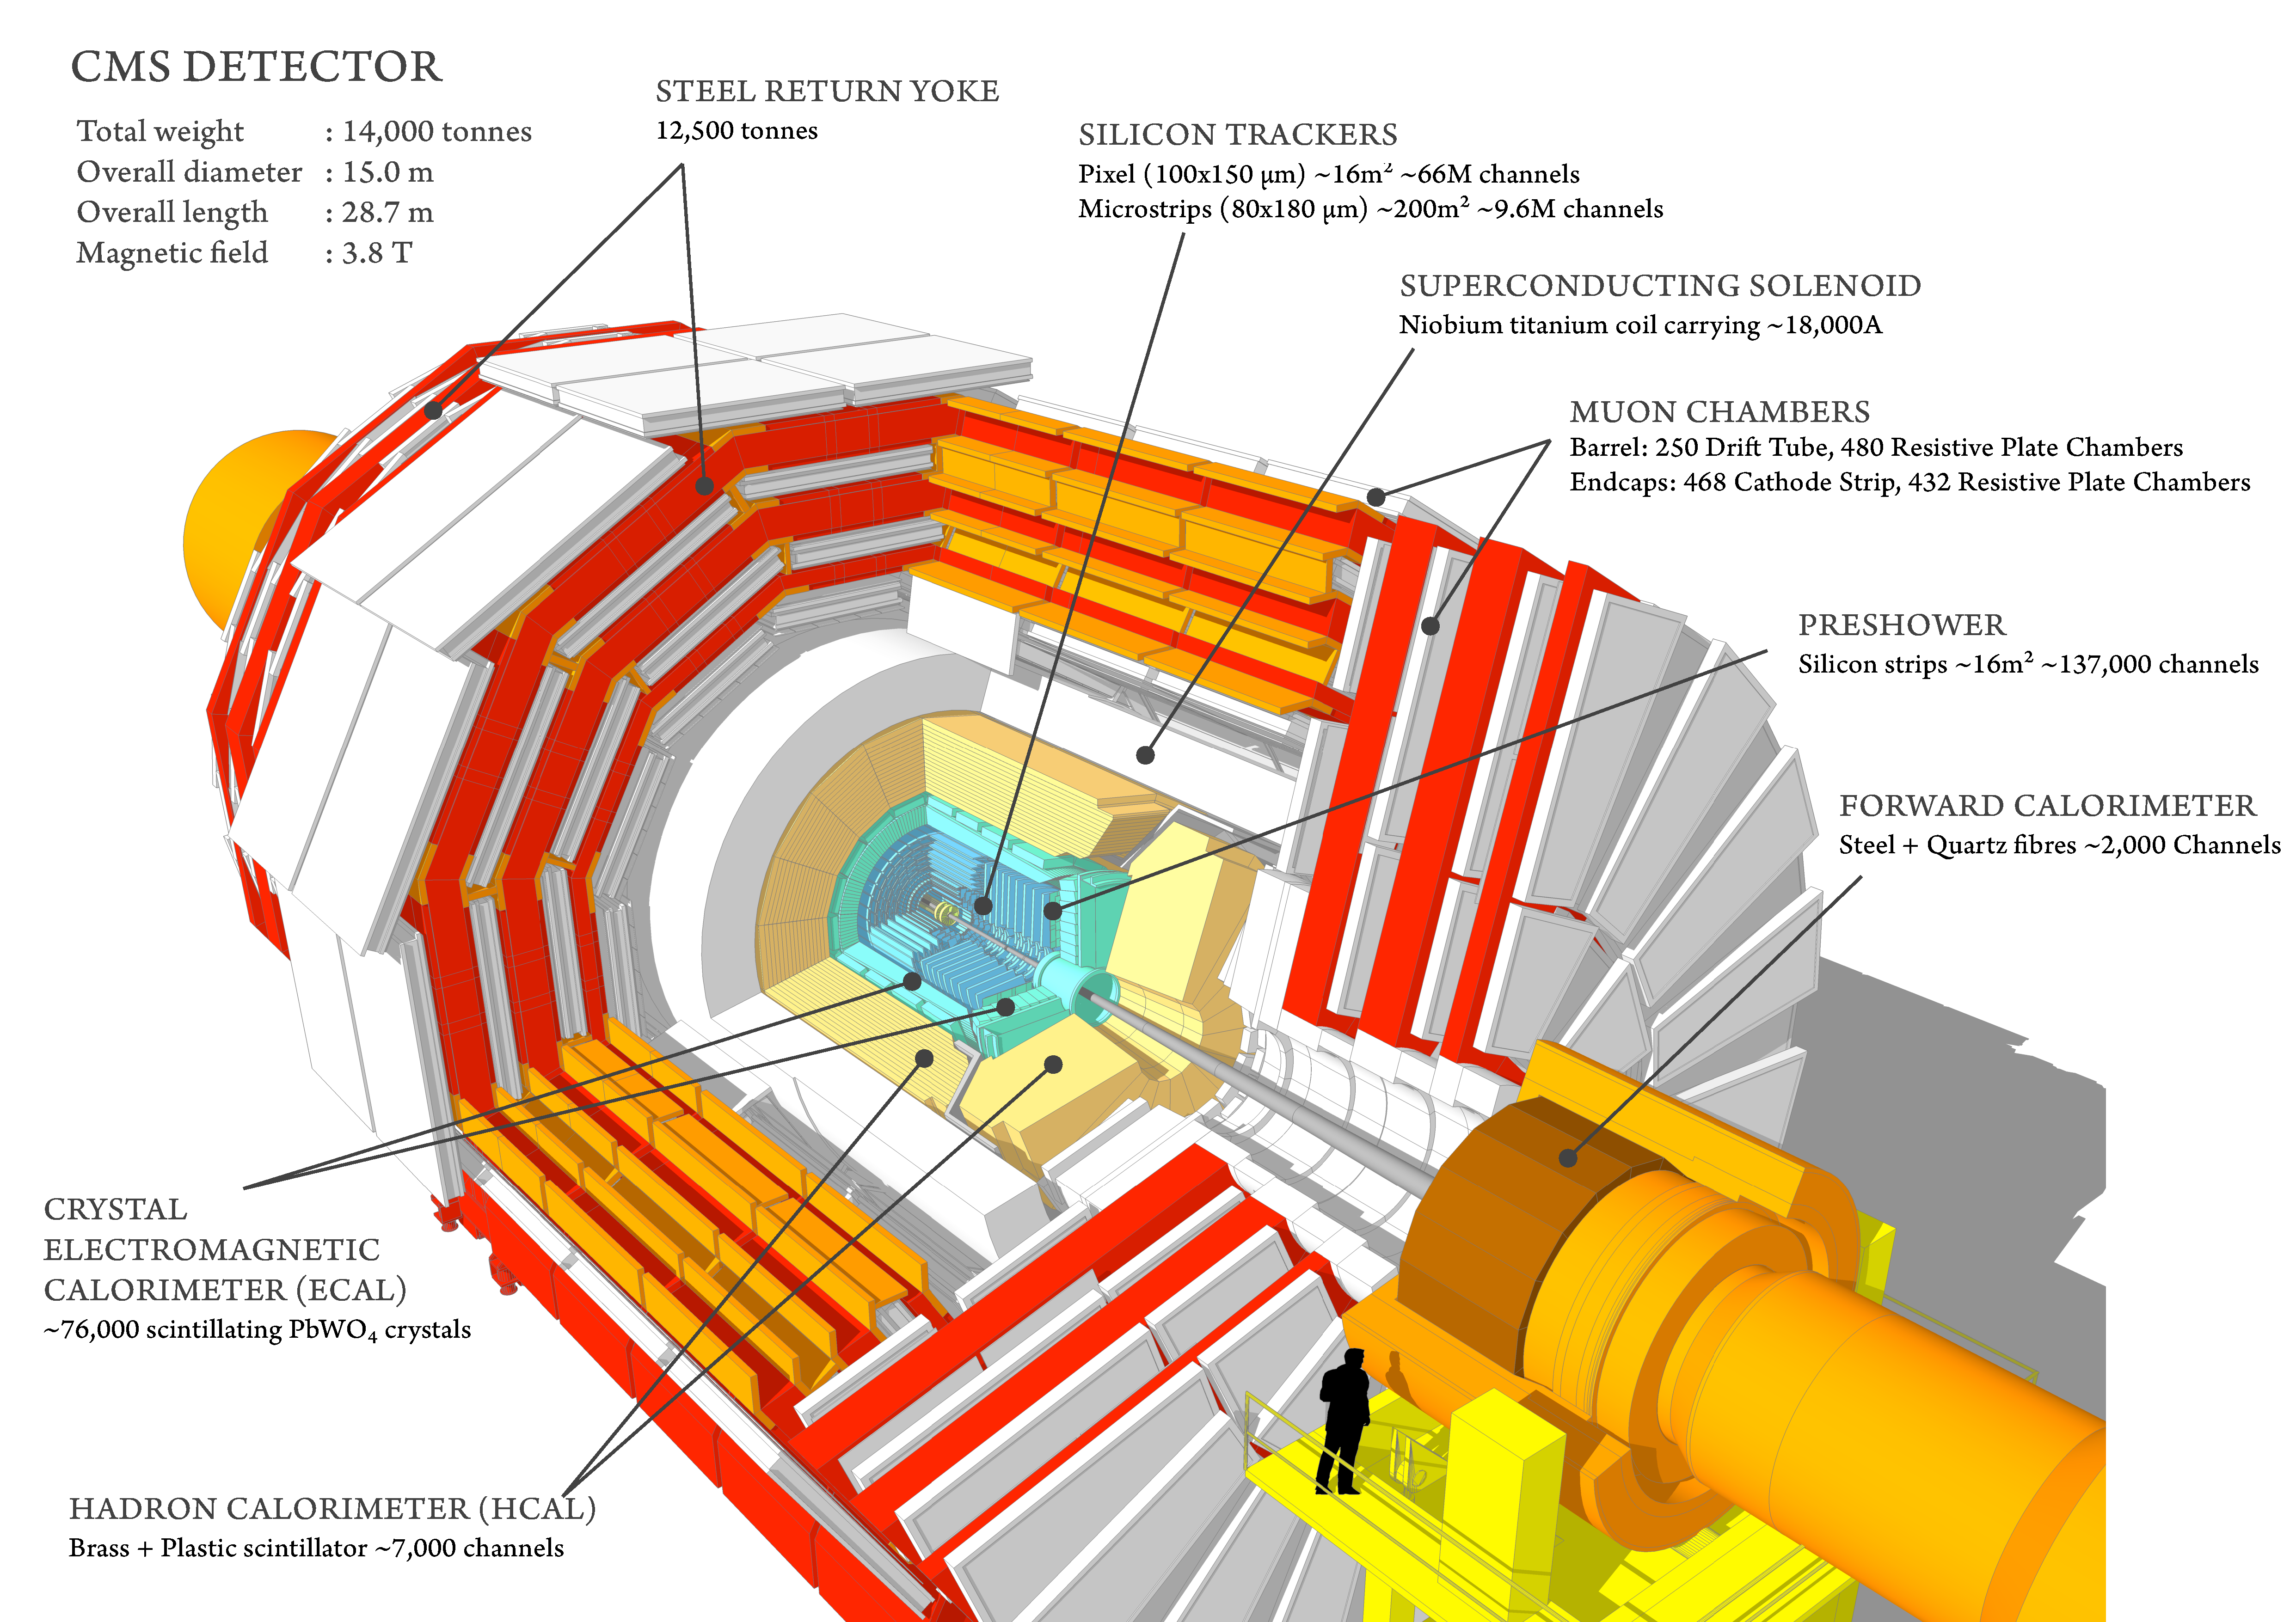
\includegraphics[width=\textwidth]{Chapters/02_Detector/Images/cms_120918_02.pdf}\hfill
     \caption[Diagrammatic sectional view of the CMS detector.]{Diagrammatic sectional view of the CMS
     detector
     \cite{Sakuma_sketchup}.}
     \label{fig:CMS_diagram}
 \end{figure}

The design of CMS is based firstly around a superconducting solenoid magnet. Around and inside the magnet are
the sub-detectors: the pixel and strip tracker, the electromagnetic calorimeter, the hadronic calorimeter, the
return yoke for the magnet and the muon detectors. The coordinate system of the detector is designated with
the origin as the intersection point of the two beams in the beampipe, the x-axis positive towards the centre
of the LHC ring, the y-axis positive vertically upwards and the z-axis pointing along the beampipe in an
anticlockwise direction. The azimuthal angle, $\phi$, is defined as the angle in the x-y plane, transverse to
the beampipe starting from the x-axis. The polar angle, $\theta$, is defined as the angle in the z-y plane
starting from the z-axis (the beampipe). The angle $\theta$ is related to the pseudorapidity, $\eta$, by the
formula $\eta=-\ln(\tan(\theta/2))$, so that $\eta$ ranges from 0 at $\theta=90~\degree$ to $\infty$ at
$\theta=0~\degree$~\cite{CMS_TDR1}. The two ends of the detector, at high $\abseta$ values, are called
the endcap regions while the central area at lower $\abseta$ values is called the barrel region. The detector
volume is often denoted in terms of $\Delta R$, with the separation between two particles 1 and 2 being
defined as
\begin{equation}
\Delta R = \sqrt{(\eta_{1} - \eta_{2})^{2} + (\phi_{1} - \phi_{2})^{2}}.
\end{equation}

\section{Sub-Detectors}
\label{s:Subdetectors}

\subsection{Tracker}
\label{ss:Tracker}

The trajectories and charges of particles created in the proton-proton collisions need to be recorded for
later use in particle reconstruction. This is achieved using the tracker section of CMS which consists of
silicon sensors in two forms: pixels and strips. The purpose of the tracker within the CMS detector is to
track the trajectory of charged particles as they travel out from the interaction point. An important
requirement of the tracker is that material budget must be low in order to allow charged particles to pass
through the tracker to outer sub-detectors while minimising multiple scattering, bremsstrahlung radiation,
nuclear interactions and photon conversions. The tracker readout chips must also be capable of distinguishing
in which bunch crossing a particle was produced (bunch-crossing identification), in order for the trigger to
remove particles from previous bunch crossings (termed out-of-time pileup) and fully reconstruct events.

The tracker is split into two parts, with an inner silicon pixel detector and an outer silicon strip detector.
A diagrammatic view of the tracker, including both pixels and strips, is shown in
Figure~\ref{fig:CMS_strip_tracker}. The inner pixel detector consists of three layers in the barrel region at
distances of 4.4\cm, 7.3\cm and 10.2\cm from the beam line with two endcap discs at each end. Each pixel
measures 100\um by 150\um. The entire pixel detector covers an area of only approximately $1\m^{2}$ and
contains 66~million pixels in total.

The strip tracker is comprised of ten layers in the barrel region at distances ranging from 20\cm to 1.1\m
from the beampipe. The four inner layers (at distances of 26\cm, 34\cm, 42\cm and 50\cm from the beampipe)
are collectively named the Tracker Inner Barrel (TIB), while the outer six layers (at distances of 61\cm,
70\cm, 78\cm, 87\cm, 97\cm and 108\cm from the beampipe) are known as the Tracker Outer Barrel (TOB).
The endcaps consist of twelve discs, three of which correspond to the Tracker Inner Discs (TID) at z-distances
from 75\cm to 100\cm, and nine to the Tracker End Caps (TEC) at z-distances between 120\cm and 280\cm
\cite{Palmonari:1260970}. The largest silicon detector ever constructed, the strip tracker contains about ten
million channels and covers an area of approximately $200\m^{2}$~\cite{CMS_experiment,CMS_TDR1}. The operating
temperature of the tracker during 2011 and 2012 was $7.4~\degreeCelsius$ and $0~\degreeCelsius$
respectively for the pixels, and $+4~\degreeCelsius$ throughout for the strips~\cite{Karancsi:2014ofa,
Butz:1497745}.

\begin{figure}[hbtp]
   \centering
     \includegraphics[width=\textwidth]{Chapters/02_Detector/Images/tracker.pdf}\hfill
     \caption[Cross sectional diagram of the CMS strip tracker.]{Cross sectional diagram of the CMS strip
     tracker; each line represents a detector module~\cite{CMS_TDR1}.}
     \label{fig:CMS_strip_tracker}
\end{figure}

As charged particles travel through these silicon sensors, electron-hole pairs are produced that induce a
current in the sensors and are processed by readout chips. This readout is carried out by the Analogue
Pipeline Voltage 25 (APV25) chip. Offline algorithms then use the data relating to which strips and sensors
received `hits' to reconstruct the tracks of charged particles and this information is later used for particle
reconstruction and identification \cite{CMS_experiment,CMS_Tracking_Early_Results}. The curving of particle
tracks within a magnetic field also allows the calculation of the particle momentum and charge, $mv=RqB$,
where $mv$ is the momentum of the particle, $R$ is the radius of curvature, $q$ is the electric charge, and
$B$ is the magnetic field strength.

% Neutral particles could also leave signals in the tracker in a small proportion of cases if the particle
% interacts with a silicon atom and/or converts to charged particles such as a photon conversion to two
% electrons. In the majority of cases, the presence of neutral particles must be detected from their energy
% deposits in the calorimeters.


%With the higher data rate expected after the LHC upgrades over the coming decade,
%pile-up will become an important issue, with approximately 20 interactions per bunch crossing even at the
%current design luminosity. This number is expected to increase to 100-200 following Long Shutdown 3.

%At higher luminosities, the occupancy (the fraction of channels with a 'hit') increases,
%which makes pattern recognition more difficult for track reconstruction algorithms and readout systems. The
%higher tracker resolution desirable for such circumstances also requires more sensors and readout chips. As a
%result, any new chip would need to be more efficient in its use of power whilst processing the data and/or
%require the associated cooling systems to be more efficient. Indeed, studies have shown that the present
%tracker could itself produce acceptable tracking performance in such conditions based on simulations of
%heavy-ion collisions, which produce similar numbers of tracks per event to that expected after the luminosity
%upgrades at the LHC [10].

%The LHC upgrades are split into 2 phases. The pixel detector will be upgraded during Phase 1, and will be an
%on-going process during both Long Shutdown 1, Long Shutdown 2 and shorter intermediate shutdowns. The strip
%detector will be upgraded during Phase 2, more specifically during Long Shutdown 3 [11][12].

The required tracker characteristics of high granularity and high resolution, fast response to process the
high data rate without losing potentially valuable information, radiation hardness and keeping detector
material to a minimum to minimise scattering without minimising the signal, resulted in silicon being chosen
to construct the tracker.

One of the advantages of using silicon over gaseous detectors is that silicon produces more charge carriers
per unit of length travelled by a particle. The silicon sensors that make up the strip tracker in the CMS
detector vary in thickness depending on their location. Sensors of 320\um thickness are utilised in the TIB
and TID, 500\um in the TOB, and a mixture of both thicknesses is used in the TEC. Thicker sensors are used in
the outer sections of the strip tracker in order to maintain a high signal to noise ratio, since the increased
strip lengths in this region lead to increased electronics noise due to higher
capacitance~\cite{CMS_experiment}.

Silicon also allows fast signal transfer, of the order of about 10\ns, as the charge carriers travel quickly
through silicon. Furthermore, the spacing between strips in a silicon sensor, known as the strip pitch, can be
manufactured to be extremely fine (<20\um). The strip pitches in the CMS strip tracker sensors vary from 80\um
to 205\um, and there are fifteen distinct pitch-length
geometries~\cite{Commissioning_and_Performance_Strip_Tracker}.

A further tracker requirement is low occupancy (the fraction of channels with a hit in an event was desired to
be 1~\% or lower at the nominal LHC luminosity) so that pattern recognition can be carried out efficiently and
so that data to be read out is manageable. In order to help maintain such a low occupancy at the nominal LHC
luminosity, the strip tracker has a high granularity, with strip lengths less than 20\cm and strip pitches
less than 205\um~\cite{Palmonari:1260970}. While high granularity is beneficial for high precision tracking,
it also results in a high number of channels, which in turn requires a large amount of electronics for readout
and leads to a high heat load.

On a global scale, the tracker data is read out using a combination of interoperating systems.
The data from the APV25 tracker readout chips is taken via optical fibres to 440 off-detector Front End
Drivers (FEDs) (tracker FEDs make up 63~\% of the total number of FEDs in CMS).
The FEDs then forward the data to the online Data Acquisition System (DAQ). In addition, off-detector Front
End Controllers (FECs) control the front-end electronics by means of approximately 350 control rings,
including triggers, clock and monitoring~\cite{CMS_experiment, Corrin}.

%As a result of the higher collision rates to be expected after
%these upgrades, the CMS tracker will require an improvement in its infrastructure because of radiation damage
%it will have suffered by that point and to ensure that it is robust enough to handle the higher levels of
%radiation after the upgrades. The pile-up is also expected to be in the range of 100 to 200 interactions per
%bunch crossing which also necessitates an improvement in the CMS tracker performance in order to ensure
%valuable data are not lost during collisions \cite{CMS_Silicon_Tracker_upgrade_for_HL-LHC}.

% Within the lattice of pure silicon, there are well-defined bands of energy levels called the conduction band
% and the valence band. The band gap is the difference in energy between these two bands and varies depending on
% the material. At absolute zero, -273$^{\circ}$C, almost all the electrons can be said to be fixed in place in
% this lattice in the valence band, meaning that if an electric field is applied across the silicon, no current
% would be able to flow. When energy is input to the system and an electron gains energy, it may be able to
% cross the band gap to the conduction band, in which case a hole would be present in its previous place in the
% valence band. At this point, both the electron and the hole are mobile and can move freely in current flow,
% for example, under the influence of an electric potential. Materials with a large band gap are insulators, and
% those with a small band gap (or even sometimes with energy bands that overlap with each other) are conductors.
% Silicon, being a semiconductor, has a 'medium' sized band gap of approximately 1.12eV. Nevertheless, the
% number of mobile electrons, above absolute zero, is still large enough to make it difficult to distinguish the
% real signal from the inherent noise in the silicon, known as leakage current (explained in Section 2.3.2).
% In order to decrease this number of free electrons and holes in silicon to obtain a much cleaner signal from a
% traversing particle (i.e. improve the signal to noise ratio), a process called doping is employed to increase
% the number of charge carriers. This involves the substituting of silicon atoms in the lattice with atoms of
% other elements like arsenic, phosphorous, boron or aluminium. In the case of the former two, both have five
% valence electrons. Four of these electrons bond to the four valence electrons present in a silicon atom,
% leaving one electron that can be easily removed from the lattice to the conduction band. This 'donation' of
% electrons to the conduction band increases the number of charge carriers. This type of silicon is called
% n-type silicon because the additional charge carriers are negative. Similarly, if boron or aluminium atoms are
% introduced to the silicon lattice, their three valence electrons bond to the electrons in a silicon atom but
% one silicon electron has nothing to bond to, creating a mobile positive hole. The addition of holes (which
% 'accept' electrons) leads to this type of silicon being called p-type because the additional charge carriers
% are positive.
% Although both p- and n-type silicon increase the number of free charge carriers, a PN-junction can be created
% by attaching a piece of n-type silicon to a piece of p-type silicon. Considering a PN-junction in isolation,
% mobile electrons from the n-type silicon would diffuse into the p-type silicon and unite with the holes from
% the p-type material, leaving behind the positively charged donor atoms. Similarly, the mobile holes from the
% p-type silicon would diffuse to the n-type silicon and leave behind negatively charged acceptor atoms. As
% these electrons and holes move to the two sides of the junction, the resulting electric field opposes the
% initial diffusion of electrons and holes, eventually reaching a state of equilibrium. Once equilibrium is
% reached, this area around the PN-junction will contain no mobile charge carriers and is called the depletion
% region.
% However, if a reverse bias voltage is applied to the silicon (a negative terminal connected to the p-type
% silicon and a positive terminal to the n-type silicon), then the electrons from the n-type silicon, rather
% than diffusing towards the junction, will be attracted towards the positive terminal. Similarly, the holes
% from the p-type silicon will be attracted towards the negative terminal, as shown in Figure 7.
% 
%  
% A higher reverse bias voltage leads to a larger depletion width as more electrons and holes are carried away
% from the junction. At high enough voltages, the width of the depletion region can be made equal to the width
% of the silicon; this voltage is known as the depletion voltage. At this stage, there are no free charge
% carriers anywhere in the silicon and it is in this state that silicon detectors are operated, thus ensuring
% that any charge carriers are only produced as a charged particle travels through the silicon. In this state,
% silicon detectors are effectively reverse biased diodes, only allowing a current to flow in one direction.
 
%Figure 8 - Basic diagram of silicon strip detector with p+ strips (green) on n-bulk (blue) [24].

% The silicon sensors in the CMS strip tracker are p+ strips (which denotes a high concentration of p-type
% impurities) on n-bulk sensors, similar to the diagram in Figure 8. As the silicon is ionised by a traversing
% particle, mobile charge carriers are created which then travel, due to the depletion voltage, to the p+ strips
% (holes) or to the backplane (electrons). As the signal will be created on a particular strip (or strips), it
% will then be possible to deduce the position of the particle.

% 2.3.2 Radiation Hardness The current tracker front-end electronics were initially designed to last about 10
% years in operation under the radiation conditions of the detector [5]. The higher radiation they will be
% subjected to as a result of the higher luminosity and higher collision energies at the HL-LHC will clearly
% impose the requirement that all components, including sensors and electronics, should be manufactured to a
% higher standard of radiation hardness. Radiation damage can occur when particles of high enough energy are
% created in the collisions at the centre of CMS that when they pass through the silicon tracker, they collide
% with atoms in the lattice. This damage is done most often by neutrons, in particular low energy neutrons from
% calorimeters and other detector elements, which interact with nuclei in the silicon and move atoms out of
% place. These atoms are knocked out of place into levels where there is usually no atom, known as interstitial
% levels. An energy of around 15eV is necessary for this to happen; generally at energies of 2keV or less only
% isolated displacements occur, whereas for energies between 2 and 12keV, one or more defect clusters will be
% created. The removal of donor atoms in this way leads to a change in the doping concentrations and eventually
% to an increase in the leakage current (current which may flow when there is no ionising particle traversing
% the silicon). A leakage current will in turn require a higher depletion voltage to remove additional electrons
% or holes captured by the electronically active defects.
% The leakage current is temperature dependent and can be mitigated by using low temperatures. The planned
% running temperature of the CMS silicon tracker in the HL-LHC is planned to be lowered from +4$^{\circ}$C to
% the region of -20$^{\circ}$C to -40$^{\circ}$C due to the benefits in terms of radiation damage. To evaluate
% the behaviour of the proposed CBC in these conditions, an environmental chamber was used to carry out tests at
% varying temperatures in this project. If a leakage current is present, this will lead to noise in the system,
% since current will always flow and any signal would sit on top of this noise. If subject to high levels of
% radiation damage, the leakage current increases to levels at which excessive amounts of power are dissipated,
% and the noise in the readout will be too high to read a clean signal.
% 
% 2.3.3 Noise The aforementioned leakage current is a result of the quantised nature of the charge carriers.
% This noise is present even when there is no signal present, and increases as radiation damage increases the
% leakage current.
% Other potential sources of noise include electronic noise caused by thermal fluctuations of the charge
% carriers. This would manifest as noise in the amplifier at the front end of the CBC and would increase
% proportionally with the capacitance of the connected input system [25]. Another contributor to noise in the
% system could be from non-linearity of the analogue to digital converter (ADC) in the CBC that converts the
% incoming analogue pulse to a digital signal [25].
% The dominant source of noise in our test system is likely to have resulted from electronic noise in the
% connected laboratory setup. In practice, the external noise under operational conditions when the CBC is
% connected to the CMS detector should ideally be maintained lower than the noise in the amplifier.


\subsection{Electromagnetic Calorimeter}
\label{ss:Ecal}
The electromagnetic calorimeter (ECAL), is a hermetic, homogeneous sub-detector constructed of scintillating
crystals of lead tungstate ($\mathrm{PbWO_{4}}$), and is the next layer outside the tracker. Any
electromagnetic particles such as electrons or photons are absorbed by the ECAL crystals which then
scintillate emitting a blue-green coloured light. These signals are then collected and converted to electrical
signals by connected photodetectors, and processed by readout electronics.

The signals in the crystals are collected by avalanche photodiodes in the barrel region and vacuum
phototriodes in the endcaps. The numbers of photoelectrons produced is dependent on temperature, with
increasing temperature resulting in a decrease in the number of electrons at a rate of
$-3.8\pm0.4\%/\degreeCelsius$. A cooling system is thus employed which maintains a stable operating
temperature of the ECAL system to within $\pm0.05\degreeCelsius$, with a nominal operating temperature of
$18\degreeCelsius$~\cite{CMS_experiment}. The energy resolution of the ECAL has been shown to follow
$\sigma_{E}/E = 2.8\%/\sqrt{E}\oplus 12\%/E \oplus 0.3\%$ where the three constant terms come from stochastic
fluctations such as photostatistics, electronics noise and temperature stability and calibration uncertainties
\cite{ECAL_calibration_and_resolution_at_7TeV}.

The barrel region of the ECAL consists of 61,200 crystals and extends up to a pseudorapidity $\eta$ of
$\pm1.479$. Each individual barrel crystal is $25.8X_{0}$ thick, where $X_{0}$ is the radiation length (the
mean distance over which a high energy electron loses all but 1/$e$ of its energy through bremsstrahlung
radiation~\cite{Agashe:2014kda}). They have individual cross sectional dimensions of $22\times22\mm^{2}$, and
are tilted with their front-faces directed towards the nominal interaction point, as can be seen in
Figure~\ref{fig:CMS_ECAL}, leading to each crystal covering $0.0174\times0.0174$ in $\eta-\phi$
plane~\cite{CMS:2010zta}. These crystals are divided into 36 groups, called supermodules, with each
supermodule consisting of 4 smaller modules. The endcaps are comprised of 7,324 crystals, cover the range
$1.479\leq\eta\leq3.0$ and are split into two halves known as ``Dees'', each divided into operating segments
of $40\degree$ each. The endcap crystals have slightly larger dimensions, having a thickness of $24.7X_{0}$
and cross sectional dimensions of $28.62\times28.62\mm^{2}$~\cite{CMS_experiment,ECAL_frontend_monitoring}.
Figure~\ref{fig:CMS_ECAL} shows the layout of the ECAL.

The crystals of high density ($8.28~\g/\cm^{3}$), short radiation length ($X_{0}=0.89\cm$), and small
Moli\`{e}re radius (a measure of the transverse dimensions of electromagnetic showers in a
material~\cite{Agashe:2014kda}) of 2.2\cm lead to a compact calorimeter with fast response time (80~\% of the
light is emitted within 25\ns) and high granularity, capable of withstanding the radiation levels within CMS.

\begin{figure}[hbtp]
   \centering
     \includegraphics[width=0.7\textwidth]{Chapters/02_Detector/Images/ECAL.pdf}\hfill
     \caption[Diagram of the ECAL showing barrel supermodules, endcaps and preshower detectors.]{Diagram of
     the ECAL showing barrel supermodules, endcaps and preshower
     detectors~\cite{ECAL_calibration_and_resolution_at_7TeV}.}
     \label{fig:CMS_ECAL}
\end{figure}

An ECAL preshower, comprised of two lead plates each followed by a layer of orthogonal silicon strip sensors
(thickness 350\mm, strip pitch 2\mm) is located between the tracker and ECAL endcaps to provide a higher
spatial resolution than the ECAL. This helps to identify, for instance, closely spaced photon pairs
originating from pion decays which may otherwise be identified as a single high-energy photon based on ECAL
energy deposits. As a photon passes through the lead, a shower of electromagnetic particles ($e^{+}e^{-}$
pairs) is produced that are detected by the silicon layers to give a measure of the energy of the photon, while the
orthogonal strips allow a position measurement. The measured energy can then be combined with the energy
measured by the ECAL.

\subsection{Hadronic Calorimeter}
\label{ss:Hcal}
The next sub-detector outside the ECAL is the hadronic calorimeter (HCAL) which works in a similar way to
the ECAL, in this case by absorbing hadron jets. The HCAL is located at a distance of 1.77~m to 2.95~m from
the beamline, with an additional outer hadronic calorimeter also installed outside the magnet due to
radial restrictions imposed by the magnet coil. The HCAL barrel (HB), outer (HO) and endcaps (HE) cover
the $\abseta$ range up to 3.0, with the forward HCAL (HF) placed at $\abseta$ up to 5.2 increasing the
coverage. Figure~\ref{fig:CMS_HCAL} shows a quarter of the HCAL endcap.

The HCAL is a sampling calorimeter, meaning it is composed of alternating absorber layers (made of brass) and
scintillator layers (made of plastic). A hadronic particle produces a shower of secondary particles when it
strikes an absorber layer. The scintillator layers in between the absorbers emit blue-violet light as the
particles traverse them. This process is repeated several times as these secondary particles pass through
successive layers of absorber and scintillator. The light in the scintillators is shifted to the green region
of the spectrum and fed via optical fibres to readout electronics where photodetectors amplify the signal and
the particle energies are measured by summing the measurements over all the layers of the hits in
the HCAL, called a ``tower''.

\begin{figure}[hbtp]
   \centering
     \includegraphics[width=\textwidth]{Chapters/02_Detector/Images/HCAL.pdf}\hfill
     \caption[A longitudinal schematic of the CMS HCAL.]{A longitudinal schematic of the CMS HCAL showing the
     location of the hadron barrel (HB), endcap (HE), outer (HO) and forward (HF) calorimeters
     \cite{CMS_experiment}.}
     \label{fig:CMS_HCAL}
\end{figure} 

\subsection{Superconducting Magnet}
\label{ss:Magnet}
The magnet of the CMS detector is the largest and highest field strength superconducting solenoid constructed
for a physics experiment in terms of bending power for physics and total stored energy~\cite{CMS_experiment}.
It can produce a magnetic field up to 4~\tesla~ (a field strength of 3.8~\tesla~ is used in normal operation)
with a stored energy of 2.7~\giga\joule~\cite{CMS_TDR1}. The cold bore, cooled to 4.5~\kelvin~ using liquid
helium, has dimensions of 12.5\m length and 6\m diameter, and weighs
220~tonnes~\cite{Cryogenic_System_for_Superconducting_Solenoid}.
Due to design constraints and structural requirements, the magnet itself provides some of the structural
strength both to support itself and to withstand its own magnetic bursting force on the coil
\cite{CMS_experiment}.

\begin{figure}[hbtp]
   \centering
     \includegraphics[width=0.5\textwidth]{Chapters/02_Detector/Images/Cold_mass.png}\hfill
     \caption[Bore of the CMS solenoid magnet in vertical position in the CMS assembly hall, SX5.]{Bore of the
     CMS solenoid magnet in vertical position in the CMS assembly hall, SX5, prior to installation \cite{CMS_experiment}}
     \label{fig:CMS_magnet_cold_bore}
\end{figure}
 
The cold bore, pictured in Figure~\ref{fig:CMS_magnet_cold_bore} in the CMS assembly hall, is enclosed in a
steel return yoke weighing 10,000~tonnes with the aim of containing and returning the magnetic field. The yoke
is interspersed with the muon chambers and is made up of 5 barrel segments and 6 endcap discs. The magnet was
designed in a manner such as to facilitate assembly at ground level prior to lowering into the CMS
experimental cavern, UX5. Despite the challenges involved in constructing such a powerful magnet, the high
bending-power created by the high magnetic field was desirable in order to provide good momentum
resolution of the tracking components.

\subsection{Muon Chambers}
\label{ss:Muon_Chambers}
Muons pass through all the previous inner sub-detectors, losing very little energy as they traverse them
(around 1\MeV/\mm on average through the whole detector), leading to the muon chambers being located outermost
in the detector. There are, in fact, three types of muon detectors in use in CMS. The endcaps contain Cathode
Strip Chambers (CSCs), the central barrel regions contain Drift Tubes (DTs), and both regions are equipped
with Resistive Plate Chambers (RPCs). These systems, in combination with the silicon tracker, are used to
determine the momentum of muons by taking advantage of their curved tracks due to the magnetic field. The
different technologies are used due to the different numbers of particles expected in different areas of the
detector and because of technological considerations regarding the physical areas to be
covered~\cite{CMS_TDR1}. Figure~\ref{fig:CMS_muon_system} shows a diagrammatic representation of one quarter
of the CMS muon detectors. The CSCs are used in the endcaps to cover \abseta values between 1.2 and 2.4 that
experience high muon rates and where the magnetic field of the solenoid is high~\cite{CMS_TDR1}. They take the
form of four disc layers each made of 2 (inner layer) or 3 (outer three layers) concentric rings. They consist
of volumes of gas in which positive wires are placed at right angles to negative copper strips. To relate
these to the name given to these detectors, the positive wires are the anodes and the negative strips are the
cathodes. As a charged particle passes through the gas it ionises gas atoms and the electrons that are knocked
out travel towards the anode wires. At the same time the resulting positively charged ions in the gas travel
towards the cathode strips. Since the wires and strips are at right angles to each other, the CSCs provide two
position co-ordinates for the passing muon. The CSC detection mechanism is a fast process so their signals are
used for muon triggering~\cite{CMS_experiment}.
 
\begin{figure}[hbtp]
   \centering
     \includegraphics[width=0.65\textwidth]{Chapters/02_Detector/Images/MuonSys-mod3.png}\hfill
     \caption[Schematic representation of a quarter of the CMS muon system.]{Schematic representation of a
     quarter of the CMS muon system \cite{Muon_tracking}}
     \label{fig:CMS_muon_system}
\end{figure}

The barrel region DTs cover \abseta values of less than 1.2, that encounter low rates of low transverse
momentum muons~\cite{CMS_TDR1}. The drift tube chambers are arranged in four cylindrical layers, or stations,
among the layers of the magnet's iron return yoke and RPC layers. The stations are slightly staggered to
ensure that even a muon of high transverse momentum will be detected by at least three of the four layers. The
drift tubes contain a mixture of argon (85~\%) and carbon dioxide (15~\%), and a positively charged stretched
wire. As a particle with a charge traverses the volume of gas, atoms in the gas are ionised and the resulting
free electrons travel along electric field lines towards the positive wire. By using the position of the
electron along the wire and the time taken for the wire to detect the electron, two coordinates of the muon
position can be deduced.
In comparison to the DTs and CSCs, the RPCs that complement them provide a better resolution in terms of time
(1\ns) but a worse resolution in terms of position, and so provide additional trigger information. As their
name suggests, they are constructed of plates, one negatively charged (cathode) and one positively charged
(anode) and made of a plastic with high resistance. In a similar process to the other muon detectors, a gas
that makes up the volume in between the plates is ionised by a passing charged muon. The resulting electrons
create an avalanche of electrons by, in turn, ionising other gas atoms; this avalanche of electrons moves
towards the anode and metal readout strips outside the plastic anode detect the signal for readout. The hit
strips pattern allows a calculation of the muon momentum which is then fed to trigger algorithms.

\subsection{Trigger and Data Acquisition}
\label{ss:Trigger}
At the design bunch crossing frequency of 40~\MHz~ and at the design luminosity of $10^{34}\cm^{-2}\s^{-1}$,
the expected number of proton-proton collisions per second is approximately $10^{9}$, translating to 21
proton-proton collisions per bunch crossing on average. Each bunch crossing produces approximately 1~MB of
data, leading to 40,000\GB/\s~ of data. This extremely large amount of data, which is impractical to record,
means that a trigger system is required to filter the events in order to record only data that are of interest
for physics analyses.

There are two levels to the CMS trigger, named Level 1 Trigger (L1) and High Level Trigger (HLT). These work
with the electronics and readout systems in place in the detector to filter the events to a practically
manageable amount for processing. In combination, these triggers reduce the data rate by at least a factor of
$10^{6}$~\cite{CMS_experiment}.

The L1 Trigger is a pipelined deadtimeless system comprised of calorimeter triggers, muon triggers and a
global trigger that works on a combination of data from the former two. The decisions made by the L1 Trigger
are carried out by custom-designed hardware processors, consisting mostly of programmable electronics such
as Field Programmable Gate Arrays (FPGAs)~\cite{1742-6596-219-3-032009}. The data from a bunch crossing are held in
pipeline buffers in the electronics on the detector (at the front end) whilst the information for the triggers
is processed in the CMS service cavern (USC) and the decisions transmitted back to the front end. The maximum
time allowed for this process for each event is 3.2\us, which is the time taken for the signals to be
transmitted via optical fibres from the detector to the processors, processing time, and transmitted back
again. This time is known as the latency~\cite{CMS_TDR1}. The L1 Trigger outputs events to the HLT at a rate
of 100~\kHz~\cite{CMS_experiment}.

As mentioned, the trigger uses calorimeter and muon chamber data to reach a decision on an event
within the required timeframe. Tracker data are not currently used since track reconstruction exceeds the
amount of time allowed for the L1 trigger decision. Good trigger performance is related to the quality of the
calorimeters and muon systems. Factors such as good momentum resolution of high momentum muons, good charge
determination of muons, good ECAL energy resolution and good missing transverse energy resolution are required
for the trigger to select interesting events. The trigger was designed as described in order to allow the CMS
experiment to meet the goals of the LHC physics programme~\cite{CMS_experiment}.

Unlike the Level 1 Trigger, the High Level Trigger (HLT) is software-based and runs offline in HLT processor
farms of about a thousand commerical processors~\cite{CMS_TDR1}. If the Level 1 produces an accept decision,
the data which was stored in buffers in the front end electronics is read into readout buffers from where the
DAQ system accesses it. The L1 output rate of 100~\kHz~ corresponds to a data rate of approximately 100\GB/\s.
The HLT software processes these events in a computer farm that carries out fast processing of offline
algorithms such as selections and object reconstructions to reduce the rate down to approximately 100~\Hz.
These accepted data are then stored on tape. The HLT algorithms are designed based on the principle of
minimising the number of objects that need to be reconstructed in order to arrive at a decision. Events are
discarded as early as possible, leading to the HLT consisting of many virtual levels that progressively use
more information from, first, the muon chambers and calorimeters, followed by pixel tracker data, and finally
full tracker information~\cite{CMS_TDR1}.

Figure~\ref{fig:single_muon_trigger_rates} shows the variation in trigger rates with increasing muon
transverse momentum at luminosities of $2\times10^{33}\cm^{-2}\s^{-1}$ and $10^{34}\cm^{-2}\s^{-1}$. The rates
for different trigger levels are shown. The L1 trigger rate begins to flatten out as the \pt threshold
increases because the lack of tracker information at L1 means that low momentum muons mis-measured as having
high momentum are not removed. Thus, increasing the threshold would have no discernible effect on reducing the
trigger rates while reducing physics performance by rejecting desirable events. In comparison, the L3 trigger
rate, which includes tracker information, continues to decrease at high muon momenta, and is able to maintain
the rate at the desired level.
% Tracker data could thus be used for improved muon momentum resolution, in addition to electron matching, for
% the application of more efficient isolation criteria, and for primary vertex identification at the L1
% stage~\cite{Klein:1628930}.
% Incorporating the tracker information in the L1 trigger at the HL-LHC would therefore be an effective method
% of maintaining the L1 trigger rate at 100kHz at higher luminosities.

\begin{figure}[hbtp]
   \centering
     \includegraphics[width=0.65\textwidth]{Chapters/02_Detector/Images/Muon_trigger_rates.png}\hfill
     \caption[Single muon HLT rates at low and high luminosities.]{Single
     muon high level trigger rates at (a) $\mathcal{L}=2\times10^{33}\cm^{-2}\s^{-1}$ and (b)
     $\mathcal{L}=10^{34}\cm^{-2}\s^{-1}$~\cite{Cittolin:578006}.}
     \label{fig:single_muon_trigger_rates}
\end{figure}

A more detailed description of the data acquisition (DAQ) system can be found in \cite{CMS_experiment}
and \cite{CMS_TDR1}.

\section{Upgrades}
\label{s:Upgrades}
The CMS experiment, along with the LHC and the other detectors are in a long term programme of upgrades and
maintenance. By 2023 the luminosity provided by the LHC is expected to be $2\times10^{34}\cm^{-2}\s^{-1}$
\cite{Technical_Proposal_Upgrade_of_CMS_Detector_through_2020}. The various runs and shutdowns until 2023 are
collectively referred to as Phase 1. In phase 2, or after 2023, long shutdown 3 is also planned to bring
further improvements and upgrades to the performance of the LHC, after which the luminosity of the LHC is
expected to reach $5\times10^{34}\cm^{-2}\s^{-1}$. The machine in this state will be known as the high
luminosity LHC, HL-LHC (also sometimes referred to as Super LHC, SLHC).

Naturally, the above dates and schedules are the latest best estimates and are liable to change over time,
particularly those further in the future, as work progresses.
\chapter{CMS Computing and Offline}
\label{c:CMS_computing_and_offline}

\section{CMS Computing}
\label{s:CMS_computing}

The CMS offline computing infrastructure takes on the workload of transferring accepted data from the triggers
to both permanent and temporary storage, of processing this data for subsequent analysis, in addition to the
production of simulated CMS data. The resources needed to process the high volumes of data involved require a
distributed computing system. The Worldwide LHC Computing Grid (WLCG) infrastructure, an international
collaboration of LHC experiments and computing centres, is employed to carry out these tasks.

CMS computing resources are primarily divided into three tiers. Tier 0 (T0) consists of only one site, at CERN
itself. The T0 centre has as its main aim to take accepted data from the detector and transfer it to permanent
storage on tape. Tier 0 computing is also responsible for reconstructing the initial RAW data into smaller
formats, by passing events through modules to produce physics objects (like electrons and jets) using
algorithms to reconstruct tracks in the silicon tracker, clusters of deposits in the calorimeters, primary and
secondary vertices, determine particle identification and to correct for detector characteristics such as
non-functioning components (see Section~\ref{s:Event_Data_Model} onwards for more details on data formats).
From the T0 centre, copies of the data in RECO and RAW format are transferred to T1 centres around the world.
Owing to its crucial role in ensuring the reliable transfer of RAW and RECO data, T0 resources are not
available for analysis by CMS users. There are seven Tier 1 centres located in various countries within the
CMS collaboration. The UK T1 centre is located at the Rutherford Appleton Laboratory in Harwell, near Oxford.
T1 centres provide reliable computing resources for data storage and processing. RAW data is spread between
them, providing a second copy of the RAW data stored at CERN. The second reconstruction step, termed RERECO,
is also carried out at T1 centres, in addition to the production of simulated data. These can then be provided
to any of the Tier 2 centres at CMS institutes (typically universities) where they may be temporarily stored.
T2 centres are also generally used to run users' final analyses and produce simulations
\cite{CMS_experiment,CMS_TDR1}.

\section{Event Data Model}
\label{s:Event_Data_Model}
Reconstructed data from CMS uses a data model based around an event, called the Event Data Model (EDM), where
one event is one crossing of proton bunches at the centre of CMS that passes the triggers. This model
is created and manipulated within a CMS software framework (CMSSW)~\cite{cmssw} written in C++, with the event
and related objects in the object-oriented data analysis framework ROOT~\cite{ROOT}.

The iterations of data from the initial recorded information to subsequent, more compact formats, are produced
by passing events through a sequence of modules. The arrangement of these data takes the form of several
layers, with the first of these being RAW. This level contains the full information from the event in CMS and
occupies approximately 1.5-2~MB/event. More information than is necessary for user analyses is included at
this level, and so the majority of CMS users will not use this data format. Reconstructed level data (RECO) is
slightly smaller in size (approximately 0.5~MB/event) and is essentially a compressed subset of the RAW data
after modules performing reconstruction have been run.

The third level, Analysis Object Data (AOD), is the smallest of the data formats, requiring approximately
100~kB/event, which is small enough to allow the entire AOD data to be stored at computing centres worldwide.
AOD format is a subset of the RECO data, and is produced by further reducing RECO, leaving only high level
physics objects (e.g. electrons, jets) which is adequate for most physics analyses. 

In the differential cross section analysis presented in this thesis, this AOD data is processed using the
Bristol Top Group's NTupleProduction code~\cite{NTT_LukeKreczko_SergeySenkin_JesonJacob_EmyrClement_2015} to
produce private ntuples which are yet again smaller in size, at approximately 3~kB/event. These ntuples are
then converted to simple ROOT histogram files after applying the required selection criteria and corrections
in the BristolAnalysisTools~\cite{BAT_LukeKreczko_JesonJacob_SergeySenkin_EmyrClement_2015}. Scripts written
in Python in DailyPythonScripts~\cite{DPS_LukeKreczko_SergeySenkin_JesonJacob_EmyrClement_2015} are then used
to produce final results plots and tables.


\section{Object Reconstruction and Identification}
\label{s:object_reconstruction_and_identification}

The process of producing a physics object such as an electron, photon or jet, from the data recorded by CMS is
known as reconstruction and is carried out by modules qknown as EDProducers within CMSSW. The three-step
process of reconstructing high level objects consists of local reconstruction within a sub detector, global
reconstruction using data from the whole CMS detector, and a final stage combining reconstructed objects from
the first two stages. The reconstruction technique used in the majority of CMS analyses is called Particle
Flow (PF) \cite{particle_flow}. PF uses information from all of the sub-detectors of CMS to identify and reconstruct
particles produced from a proton-proton collision.

\subsection{Track Reconstruction}
\label{ss:track_reconstruction}
Algorithms performing local track reconstruction execute a scan to identify tracker modules that receive a
higher than threshold signal. Clusters are then constructed by adding adjacent strips or pixels to the
originally identified seed strip or pixel. In order to reconstruct complete tracks to obtain the position and
momentum of the charged particle, algorithms based on specific requirements such as high or low transverse
momentum tracks are used. These algorithms in CMS are collectively known as the Combinatorial Track Finder
(CTF).

Multiple passes of the CTF reconstruction software are carried out to reconstruct tracks, in a process called
iterative tracking. The earliest iterations identify tracks that are easy to find such as high \pt tracks
originating near the interaction point. As these tracks are reconstructed, the corresponding hits are removed
from consideration in subsequent iterations, making it simpler for later iterations to identify tracks that
are more difficult to find such as those of displaced particles or with low \pt.

Six iterations are carried out in total, and each iteration can be split into four steps. Seeds are created
using 2 or 3 hits to produce intial track candidates. The seed gives an estimate of the trajectories of the
potential track candidates. A Kalman Filter \cite{kalman_filter, Speer:927395} based track finding algorithm
then looks for further hits along an extrapolated path of the seed trajectory. A track fitter is then run
using information from the previous steps to produce final values for trajectory parameters. The fourth and
final step then rejects tracks which fail specified quality checks \cite{track_reconstruction}.

\subsection{Pileup Subtraction}
\label{ss:pileup_subtraction}
When reconstructing an event in CMS, all vertices (points from which multiple tracks originate) in the event
must be reconstructed. By ordering the vertices by the sum of the transverse momenta of their tracks, it is
possible to identify the the vertex of interest for physics analyses, known as the primary vertex (PV), as the
vertex with the largest transverse momentum. The particle flow algorithm reconstructs objects, starting with
those coming from the primary vertex, followed by other vertices (known as pileup). The reconstructed objects
from the PV can be affected by the number of other vertices present in the event. For example, the jet
momentum and lepton isolation could both increase with high pileup. This can, in turn, lead to signal events
not passing selection requirements because a truly isolated lepton from the PV may appear not to be isolated.
In addition, a larger number of events from background processes may pass selection requirements due to low
energy jets appearing to have a higher energy. Hence, pileup subtraction, the removal of charged particles
coming from vertices other than the PV is implemented to reduce these effects.

Neutral particles, however, pose a more difficult problem since they leave no tracker information for the
reconstruction algorithms to easily identify their origin. One method of removing such particles from an
event, known as the $\Delta\beta$ correction, uses the fact that the estimated average energy in an event from
neutral particles is half that from charged particles. Thus, it can be estimated that 0.5 times the charged
particle energy comes from neutral particles. The second method, known as $\rho$ correction, subtracts an
average transverse momentum coming from pileup per unit area. While the two methods produce similar results,
the $\rho$ correction is used to correct the electron isolation and the $\Delta\beta$ correction is used to
correct the muon isolation in the differential cross sections analysis presented in this thesis, as
recommended by the CMS TOP physics analysis group.

\subsection{Electron Reconstruction}
\label{ss:electron_reconstruction}
ECAL local reconstruction algorithms calculate the time of arrival, position and the energy of deposits. After
grouping together deposits in neighbouring crystals to form clusters, deposits are then matched to deposits in
the HCAL, forming a Calo Tower. Electrons are, typically, completely stopped in the ECAL and deposit their
energy in a narrow cluster of crystals.

However, electrons can interact with the material between the interaction point and the ECAL, emitting a
photon via bremsstrahlung radation. Similarly, photons can convert to an elecron-positron pair ($e^{+}e^{-}$).
Both of these processes result in ECAL deposits with a larger spread in $\phi$ because of the strong magnetic
field in the inner section of CMS containing the tracker. In the case of photons, several clusters are grouped
together to form superclusters, which are then corrected for their energies to obtain the energies of the
original photon \cite{photon_reconstruction}.

Electron reconstruction in the ECAL is carried out by two methods. The first matches superclusters with a
trajectory compatible with two or three pixel detector hits and the interaction point. The second matches the
supercluster to tracker tracks to identify electrons (and in the case of electrons emitting bremsstrahlung
radiation, tracks with a low number of hits) \cite{electron_reconstruction}. Combining the seeds from the two
methods, a Gaussian-Sum Filter, a generalisation of the Kalman Filter algorithm, is used to reconstruct
electron paths \cite{electrons_GSF}.

Since other objects can leave similar signatures in the detector to electrons, such as jets or electrons from
photon conversions, candidates are required to satisfy additional requirements of identification and
isolation. Several electron identification methods exist and are used in CMS analyses. The top cross sections
analysis in this thesis uses the multivariate identification (MVA ID). As the name suggests, this approach
uses a multivariate analysis, with track, track quality, and supercluster variables as input, to produce a
discriminator value, with higher values indicating a higher likelihood for a candidate to be a real electron.
The MVA ID algorithm is optimised for identifying electrons from W and Z boson decays, and separately for
triggering and non-triggering electrons~\cite{electron_reconstruction}.

The isolation of an electron is defined as the activity within a cone surrounding the electron. Isolation is
used as an additional criterion to select electrons, in particular to distinguish electrons promptly produced
in a proton-proton collision. Such isolated electrons would have less activity in its vicinity than electrons
from within a jet, which could originate from leptonically decaying b hadrons, and jets faking electrons. Two
methods exist in CMS of calculating the isolation of a particle: detector based isolation and particle based
isolation. The detector based method is defined in each sub detector as the sum of the momenta or energies in
a cone of $\Delta R = 0.3$ around the electron. The particle based method uses the total transverse energy of
PF reconstructed particles within a cone of $\Delta R = 0.3$ and can remove activity coming from collisions
other than the hard proton-proton interaction of interest. By normalising this isolation to the momentum or
energy of the electron, a relative isolation is obtained, relating the cone activity to the electron.
Termed PFRelIso, it is this relative isolation that is used in the cross section analysis to select
electrons.
% can improve signal efficiency

In order to avoid the selection of electrons originating from a photon conversion, a veto can be placed on a
second electron in the event. However, since the two electrons in a photon conversion may not necessarily have
equal transverse momentum, \ie one may have a very low \pt, such a veto may be insufficient, and so further
techniques to identify conversion events are used. Firstly, since an electron from a conversion would be
produced at some distance from the interaction point and in the detector material, eliminating candidates with
missings hits in the pixel tracker helps to distinguish such electrons from promptly produced electrons. In
events in which the conversion occurs in the beam pipe or if the electron is matched to unassociated pixel
hits, this method can also be insufficient, so an additional track matching step is used. Tracks are matched
in pairs and following geometrical cuts, can be removed if they appear to originate from a conversion
\cite{electron_reconstruction}.

\subsection{Muon Reconstruction}
\label{ss:muon_reconstruction}
Local reconstruction in the muon chambers provides hit position and time of arrival of a muon. This
information from the DTs and CSCs is then amalgamated to create muon track hits and segments, which are then
used by the muon global reconstruction algorithms to reconstruct ``standalone'' muons. An inner detector
segment is used as a seed for a Kalman Filter~\cite{kalman_filter, Speer:927395} and possible trajectories are
generated. By removing hits which are unlikely to have come from the track in question, the likely trajectory
is constructed layer-by-layer. A final fit is carried out, including an extrapolation to the interaction point
for greater momentum resolution.

Muons are also independently reconstructed in the tracker. These tracker tracks can therefore be combined with
the aforementioned muon chamber information, where the magnetic field is only 2~\tesla, to improve the \pt
resolution of muons, as seen in Figure~\ref{fig:muon_momentum_resolution}.

\begin{figure}[hbtp]
   \centering
     \includegraphics[width=0.65\textwidth]{Chapters/02_Detector/Images/muon_momentum_resolution.png}\hfill
     \caption[Muon transverse momentum resolution using muon system and the tracking system.]{Muon transverse
     momentum resolution as a function of muon transverse momentum using the muon system only, using inner tracking only,
     and using both~\cite{Chatrchyan:2012xdj}.}
     \label{fig:muon_momentum_resolution}
\end{figure}

Two methods are employed to combine the information from the two sub-detectors. \textit{Global muon
reconstruction} matches a tracker track to a standalone muon track and carries out a fit of the resulting
\textit{global muon} track. The second method, \textit{tracker muon reconstruction}, extrapolates tracker
tracks outwards to the muon chambers and accepts a muon candidate if a DT or CSC matching track is found and
the muon \pt is greater than 0.5\GeV~\cite{muon_reconstruction}.

For triggering, the \pt of a muon is first estimated using the information available at Level 1 from all three
types of muon detectors. At HLT level, the muon candidates from Level 1 are further refined using track
finding and fitting, but still using only information from muon chambers, leading to Level 2 muons. As
mentioned in Section~\ref{ss:Trigger}, due to the time constraints required of the L1 trigger, full tracker
data are not currently used. However, tracks of Level 2 muons are extrapolated into the tracker systems and a
localised track finding algorithm is run to identify only nearby tracker hits. A track matching that of a
Level 2 muon leads to a Level 3 muon. %See Emyr's thesis P45 top for details.

\subsection{Jet Reconstruction}
\label{ss:jet_reconstruction}
As quarks produced in proton-proton interactions (except the top quark) hadronise~\cite{Griffiths:1987tj},
jets of particles are formed in the direction of travel of the quark. The time of arrival, position and the
energy deposited by hadronic objects are locally reconstructed in the HCAL. If the deposit matches an ECAL
deposit, a Calo Tower is formed for later use in jet reconstruction algorithms.

The PF algorithm performs the reconstruction of particles in the jet, and the \antikt algorithm is used to
perform the clustering of these particles into jets. The \antikt algorithm, explained in detail
in~\cite{Cacciari:2008gp}, is one of several jet algorithms that exist in CMS to combine reconstructed
particles into jets. It defines a distance $d_{ij}$ between reconstructed particles as
\begin{equation}
%\begin{center}
d_{ij} =
min\left(\frac{1}{p_{T,i}^{2}},\frac{1}{p_{T,j}^{2}}\right)\frac{(\eta_{i}-\eta_{j})+(\phi_{i}-\phi_{j})^{2}}{R^{2}}.
%\end{center}
\end{equation}
$p_{T,i}$ and $p_{T,j}$ are the transverse momenta of the two particles $i$ and $j$, $\eta_{i}$ and $\eta_{j}$
are the rapidities, $\phi_{i}$ and $\phi_{j}$ are the azimuth angles and $R$ is the radius of the jet cone.
The \antikt algorithm iteratively clusters together particles with the smallest $d_{i,j}$ between them until
all jets are reconstructed and there are no particles remaining. Events will usually consist of a small number of
high-\pt (hard) particles and a large number of low-\pt (soft) particles. The distance between hard particles
is typically small, and the distance between softer particles is larger. Soft particles tend to
cluster around hard particles first, before clustering with other soft particles.

While the PF anti-$k_{t}$ jets show high jet matching efficiency on Monte Carlo simulation samples,
corrections are applied based on the jet $\pt$ and $\eta$ to correct for mismeasurements in the
detector and thereby improve the agreement between generated and reconstructed particle flow jets. The
factored approach to CMS jet energy corrections is comprised of three parts:
\begin{enumerate}
  \item {L1 Pile Up: corrects for additional energy from charged particles from pile-up in the event
  \ref{ss:pileup_subtraction}.}
  \item {L2 Relative Jet Correction: corrects the reconstructed energy to match the generated jet with respect
  to $\eta$.} %to flatten the jet response in the ecal eta
  \item {L3 Absolute Jet Correction: corrects the reconstructed energy to match the generated jet with respect
  to $\pt$.} %to flatten the jet response in the ecal pt
  \item {L2L3Residuals: reduces any residual differences between the reconstructed and generated
  jet due to simulation not being perfectly tuned to data. This correction is applied to data only.}
  %https://twiki.cern.ch/twiki/bin/viewauth/CMS/IntroToJEC
\end{enumerate}
In order to identify jets in the differential cross sections analysis, further identification criteria are
used to reduce electronic noise, to reduce the number of electrons mis-identified as jets and, in so doing, to
ensure the selection of high quality jets. The requirements, which are known as the loose PF Jet ID, are:

\begin{itemize}
  \item at least one constituent particle
  \item the neutral hadron energy fraction (NHF) must be $<0.99$
  \item for jets with \abseta$<2.4$, the charged hadron energy fraction (CHF) must be $>0$
  \item the neutral electronmagnetic energy fraction (NEF) must be $<0.99$
  \item for jets with \abseta$<2.4$, the charged electronmagnetic energy faction (CEF) must be $<0.99$
  \item for jets with \abseta$<2.4$, the number of charged hadronic constituents (NCH) must be $>0$
\end{itemize}

\subsubsection{B Jets}
\label{sss:b_jets}
The process of identifying jets coming from \bquarks is known as \btagging and is very important in top quark
physics due to the decay of the top to a \W boson and a \bquark. Effective \btagging can therefore help to
appreciably reduce background processes in an analysis. A description of \btagging, the several algorithms
available in CMS, relevant event variables, and a performance comparison, is given in
Chapter~\ref{c:b_tagging_study}.

\chapter{The Standard Model}
\label{c:the_standard_model}

\section{Introduction}
\label{s:standard_model_intro}

The Standard Model is the name given to the theory developed during the course of the 20th century, which
describes the elementary particles that make up all known, observable matter, and the three fundamental forces
they interact by (electromagnetic, weak and strong forces). The Standard Model does not, however, describe the
gravitational force as it is difficult to model mathematically at a quantum scale.
% The theory is a combination of the theory of the electroweak interaction and the theory of the strong
% interaction
The Standard Model puts forward twelve fermions, with a spin quantum number of $\frac{1}{2}$, as the matter
particles, split into two groups of six quarks and six leptons, all of which are split into three generations.
The six quarks are classified according to their charge and flavour: up, down, charm, strange, top and beauty
quarks. The leptons are in turn classified according to their charge and flavour: electron, muon or tau
leptons, together with their corresponding neutrinos). Neutrinos, although originally thought to be massless,
are now believed to carry mass due to the observation of the oscillation of neutrinos between different
flavours. Table~\ref{tab:standard_model} shows these particles of the Standard Model in their respective
generations in tabular form. All of these particles have a respective antiparticle which has identical quantum
numbers except opposite electric charge.

\begin{table}[hbth]
\centering
\begin{tabular}{lllll}
\hline
Generation & Flavour & Charge / $e$ & Spin & Mass /\MeV \\
\hline
\hline
\multicolumn{5}{c}{\textbf{Leptons}} \\
\hline
\multirow{2}{*}{I} & electron (e) & -1 & $\frac{1}{2}$ & 0.511 \\
 & electron neutrino ($\nu_{e}$) & 0  & $\frac{1}{2}$ & $<2 \times 10^{-6}$ \\
\hline
\multirow{2}{*}{II} & muon ($\mu$) & -1 & $\frac{1}{2}$ & 105.66 \\
 & muon neutrino ($\nu_{\mu}$) & 0 & $\frac{1}{2}$ & $<2 \times 10^{-6}$ \\
\hline
\multirow{2}{*}{III} & tau ($\tau$) & -1 & $\frac{1}{2}$ & $(1.777 \pm 0.16) \times 10^{3}$\\
 & tau neutrino ($\nu_{\tau}$) & 0 & $\frac{1}{2}$ & $<2 \times 10^{-6}$ \\
\hline
\hline
\multicolumn{5}{c}{\textbf{Quarks}} \\
\hline
\multirow{2}{*}{I} & up (u) & $+\frac{2}{3}$ & $\frac{1}{2}$ & $2.3^{+0.7}_{-0.5}$ \\
 & down (d) & $-\frac{1}{3}$ & $\frac{1}{2}$ & $4.8^{+0.5}_{-0.3}$ \\
\hline
\multirow{2}{*}{II} & charm (c) & $+\frac{2}{3}$ & $\frac{1}{2}$ & $(1.275 \pm 0.025) \times 10^{3}$ \\
 & strange (s) & $-\frac{1}{3}$ & $\frac{1}{2}$ & $95 \pm 5$ \\
\hline
\multirow{2}{*}{III} & top/truth (t) & $+\frac{2}{3}$ & $\frac{1}{2}$ & $(173.21\pm{0.51}\pm{0.71}) \times 10^{3}$ \\
 & bottom/beauty (b) & $-\frac{1}{3}$ & $\frac{1}{2}$ & $(4.18^{+0.03}_{-0.03}) \times 10^{3}$ \\
\hline
\hline
\multicolumn{5}{c}{\textbf{Bosons}} \\
\hline
Force & Gauge Boson(s) & Charge / $e$ & Spin & Mass /\GeV \\
\hline
Weak & $\W^{+} / \W^{-}$ & +1/-1 & 1 & $80.385\pm0.015$ \\
Weak & $\Z^{0}$ & 0 & 1 & $91.188\pm0.002$ \\
Electromagnetic & photon ($\gamma$) & 0 & 1 & 0 \\
Strong & gluon (g) & 0 & 1 & 0 \\
%Gravitation & graviton & 0 & 2 & 0 \\
- & Higgs (H) & 0 & 0 & $125.7\pm0.4$ \\
\hline
\end{tabular}
\caption{Fundamental fermions, split into their three generations, and bosons of the Standard Model. The
graviton is curently only hypothesised. Particle properties taken from \cite{Agashe:2014kda}.}
\label{tab:standard_model}
\end{table}



All known, observable matter in the universe is composed of the aforementioned twelve fermions or their
antiparticles. The only particles which are stable are the proton, which is made of two up quarks and a down
quark; the neutron, which is made of one up quark and two down quarks; and the electron. All other particles
are unstable and decay; they are produced only in particle colliders such as the Large Hadron Collider, or in
cosmic radiation. Quarks also carry the charge of the strong force, termed 'colour', of red, green or blue.
The only quark which does not 'hadronise' (form bound colourless states) is the top quark which has a
very short lifetime of $\approx 5 \times 10^{-25}s$ \cite{Agashe:2014kda} due to its large mass.

These fermions interact via the integer spin (spin 1) gauge bosons of the three fundamental forces. Electron,
muon and tau leptons interact via the electromagnetic and weak forces; their neutrinos, since they carry no
electric charge, interact only via the weak force; and the quarks interact via the electromagnetic, weak and
strong forces. Each of the forces are mediated by gauge bosons that are the 'force carriers', and lead to the
formation of hadrons and atoms. The mediator of the strong force is known as the gluon, that of the
electromagnetic force is the photon and those of the weak force are the $\W^{+}$, $\W^{-}$ and $\Z$ bosons.
Table~\ref{tab:standard_model} shows the gauge bosons and their properties.

The range of action of the boson determines the interaction range of the force it carries. Heavier bosons,
like the $\W^{+}$, $\W^{-}$ and $\Z$ bosons, have a short range of action, while massless bosons such as
photons and gluons have a theoretically infinite range. In reality, this is not the case because the gluons
themselves carry the strong colour charge and so interact with each other, reducing their interaction range.
The range of the  fundamental forces is quantified by their coupling strength, denoted $\alpha$. Taking the
strength of the strong force as the baseline, the relative strength of the electromagnetic force is $10^{-2}$,
that of the weak force is $10^{-13}$ and the strength of the gravitational force is $10^{-42}$
~\cite{Griffiths:1987tj}. The electromagnetic coupling strength, also known as the fine-structure constant, is
defined at low energies as $\alpha_{em} = \frac{e^{2}}{4\pi}\approx \frac{1}{137}$. Although the strong force
is the strongest force, it has a limited range of only an estimated $10^{-15}$m, and the weak force has an
estimated range of $10^{-18}$m, while the electromagnetic and gravitational forces have infinite range.

The Higgs boson, whose discovery was announced in July 2012 by the CMS and ATLAS experiments at the LHC, is
the latest component of the Standard Model to be discovered \cite{Chatrchyan:2012xdj, Aad:2012tfa}. The
mechanism of electroweak symmetry breaking through which other particles acquire mass is due to this Higgs
field.

\subsection{Gauge Principle}
\label{ss:gauge_principle}
The underlying mathematical model of the Standard Model is a Quantum Field Theory (QFT) combining special
relativity and quantum mechanics. All interactions in the the SM must conserve the kinematic quantities energy
and momentum. In addition, the electromagnetic and strong forces conserve the dynamical quantities charge,
colour, baryon number, lepton number and quark flavour. The weak force, if mediated by a charged propagator
($W^{\pm}$), can allow the violation of quark flavour, meaning a quark can decay into another flavour quark.

The laws of conservation occur as a result of underlying symmetries in the theories; for instance, energy
conservation stems from time symmetry and angular momentum conservation is a result of rotational symmetry.
In addition to these classical symmetries, a quantum field theory can also possess gauge symmetries. The
principle of gauge invariance refers to field theories in which the Lagrangian, which summarises the dynamics
of the system, is invariant under local transformations (transformations that are a function of, and therefore
different at all space-time points in, a field). The collection of all such transformations, called gauge
transformations, are called the Lie group. If the Lie group is commutative, \ie any order of application of
the symmetry transformations produces the same result, the theory is termed Abelian. Conversely, if the group
is non-commutative, the theory is non-Abelian. Each Lie group has an associated generator, and each generator
has a corresponding vector field, or gauge field, whose purpose is ensuring invariance under local
transformations. The quanta of these fields are the gauge bosons of the Standard Model. Note that the converse
of local transformations are global transformations, in which the transformation takes place instantaneously
at all space-time points.
% However, the speed of any tranformation is limited to c, the speed of light, and so a more realistic local
% transformation is interesting to consider.

Group transformations can be represented as groups of $n \times n$ matrices which possess properties such as
unitarity ($U$) and orthogonality ($O$). A group of matricies with determinant 1 is called 'special' ($S$),
leading to further groups of $SU(N)$ and $SO(N)$. The Standard Model is comprised of electroweak theory
(combining electromagnetism and weak theory) a gauge group of $SU(2) \times U(1)$ and the theory of strong
interactions that has a gauge symmetry of $SU(3)$. The Standard Model is therefore a gauge theory based on the
gauge group $SU(3) \times SU(2) \times U(1)$.

\subsection{Quantum Electrodynamics}
\label{ss:quantum_electrodynamics}

Quantum electrodynamics (QED) is a component theory of the Standard Model that governs the interactions of
electrically charged particles. The simplest electromagnetic process is shown in
Figure~\ref{fig:qed_processes}a, and all real processes are made of some number of these processes combined
together, such as electron-positron annihilation shown in Figure~\ref{fig:qed_processes}b.

\begin{figure}[hbtp]
   \centering
     \includegraphics[width=0.3\textwidth]{Chapters/03_Theory/Images/e_e_gamma}\hfill
     \includegraphics[width=0.5\textwidth]{Chapters/03_Theory/Images/e_e_gamma_e_e}
     \caption[Elementary electromagnetic processes.]{(a) the elementary electromagnetic process of an electron
     emitting a photon and (b) electron-positron annihilation.}
     \label{fig:qed_processes}
\end{figure}

The sum of all possible orders of Feynmann diagrams for a possible interaction is the representation of the
real process. In practice, since at low energies, each vertex contributes a factor of $\alpha$
($=\frac{1}{137}$, the fine structure constant, the coupling constant of the electromagnetic force),
additional Feynmann diagrams with more than a few vertices contribute negligibly to the process and are often
ignored.

The coupling strength of a force can be further explained in terms of vacuum polarisation. This refers to the
phenomenon of electron-positron pairs and photons being spontaneously created and absorbed by an electron.
These virtual particles, which would be represented in Feynmann diagrams as closed loops, shield the original
electron leading to the electron charge being measured at a lower value than its true charge. This measured
value is called the effective, or 'screened', charge. As a result, the coupling strength of the
electromagnetic force decreases as a function of distance.

The mathematical formulation of QED stems from the Dirac equation, which describes the Lagrangian for a
spin-half (Fermionic) field $\psi$.

\begin{equation}
\calL = i (\hbar c) \bar{\psi} \gamma^{mu} \partial_{\mu} \psi - (mc^{2}) \bar{\psi} \psi
\end{equation}

Here, $\hbar$ is the reduced Planck's constant, $\mu$ are the Lorentz indices and $\gamma^{mu}$ are the gamma
(or Dirac) matrices. Under a global transformation of a phase $i \alpha$, 

\begin{equation}
\psi(x) \rightarrow \psi'(x) = e^{i\alpha}\psi(x), \bar{\psi} \rightarrow \bar{\psi}'(x) =
e^{-i\alpha}\bar{\psi}(x)
\end{equation}

this Lagrangian is invariant (\ie under a global transformation of the $U(1)$ group, since this is
equivalent to multiplication of the field $\psi$ by a $1 \times 1$ unitary matrix). However, under a local
gauge transformation by a phase of $i\alpha(x)$, the symmetry is no longer true since the partial derivative

\begin{equation}
\partial_{\mu}(e^{i\alpha(x)}\psi) = i(\partial_{\mu}\alpha(x))e^{i\alpha(x)}\psi +
e^{i\alpha(x))}\partial_{\mu}\psi ,
\end{equation}

meaning the Lagrangian is not invariant:

\begin{equation}
\calL \rightarrow \calL - \bar{\psi}(x)\gamma^{\mu}\psi(x)[\partial_{\mu}\alpha(x)].
\end{equation}

Local symmetry can be maintained in this case if a new gauge field, $A_\mu$, is introduced to the Lagrangian
by means of a covariant derivative $D_\mu$:

\begin{equation}
D_{\mu} = \partial_{\mu} + ieA_{\mu}.
\end{equation}

Under the local transformation, $A_{mu}$ tranforms as

\begin{equation}
A_{\mu} \rightarrow A_{\mu}' = A_{\mu} - \frac{1}{e}\partial_{\mu}\alpha(x).
\end{equation}

If the partial derivatives in the Dirac equation are now replaced with the covariant derivatives, the
invariant Lagrangian is obtained:

\begin{equation}
\calL = i (\hbar c) \bar{\psi} \gamma^{mu} \partial_{\mu} \psi - e \bar{\psi} \gamma^{\mu} \psi A_{\mu} -
(mc^{2}) \bar{\psi} \psi - \frac{1}{4}F^{\mu\nu}F_{\mu\nu}.
\end{equation}

In this way, the principle of local gauge invariance under the $U(1)$ group is used to obtain the final
Lagrangian, that of quantum electrodynamics. The physical interpretation of the gauge field $A_{\mu}$ is the
photon, which couples to charged particles (electrons and positrons) with a coupling strength proportional to
the charge. The term $\frac{1}{4}F_{\mu\nu}$ is an additional term to account for the kinetic energy of the
free particle of the new gauge field, \ie the photon; and there is no term giving the photon mass.

% \begin{equation}
% F_{\mu\nu} = \partial_{\mu}A_{\nu} - \partial_{\nu}A_{\mu}.
% \end{equation}

In this way, the principle of local gauge invariance under the $U(1)$ group is used to 
introduce additional
fields to a Lagrangian in order to make it covariant with respect to a group  $U(1)$ local gauge invariance

\subsection{Electroweak Theory}
\label{ss:electroweak_theory}

The unification of the electromagnetic and weak forces in the 1960s provided a more complete theory of
fundamental particles. This unification takes the form of an $SU(2) \times U(1)$ gauge group correlating the
electromagnetic and weak forces, and can be constructed in a similar way to the QED formalism in
Section~\ref{ss:quantum_chromodynamics}. 

First, it is necessary to define isospin, $I$ an abstract fundamental property of fundamental particles that
is conserved in weak interactions. Similarly, weak hypercharge, $Y$ is also a quantum property, defined as
$Y_{W} = 2(Q-I_{3})$, where $Q$ represents the charge of the particle and $I_{3}$ is the third component of
isospin. $I_{3}$ takes a value of $\frac{1}{2}$ for up, charm and top quarks and for neutrinos; and
$-\frac{1}{2}$ for down, strange, beauty and other leptons other than neutrinos.

It has been shown empirically that the weak interaction exhibits violation of parity ($P$) and interacts
only with left-handed particles via the charged gauge bosons ($W^{\pm}$). Hence, the fields representing
fermions are split into left handed and right handed components by defining a left handed doublet
containing the left handed electron and left handed neutrino, and a right handed singlet containing the right
handed electron:
\begin{equation}
\chi_{L} = \left( \begin{array}{c} \nu_{e} \\ e \end{array}\right)_{L}, e_{R}
\end{equation}
Here, the left handed doublet has $I=\frac{1}{2}$, and the right handed lepton has $I = 0$. Similar doublets
can be constructed for the other generations of leptons ($\mu$ and $\tau$) and quarks in their pairs of three
generations ($ud$, $cs$ and $tb$). Right handed neutrinos, which would have $I=0$ and $Y=0$, do not exist in
the Standard Model. %as they would not interact with any of the force mediators.

Four additional massless fields and their associated currents are introduced in order to impose invariance:
$W_{\mu}^{1}$, $W_{mu}^{2}$, $W_{mu}^{3}$ and $B_{\mu}$. The $W_{\mu}$ fields form a triplet that transforms
according to the $SU(2)$ group, and undergoes interactions with the third isospin component $I_{3}$. The
$B_{\mu}$ field similarly transforms by the unitary group $U(1)$, and interacts with the weak hypercharge $Y$.
These additional fields lead to the construction of three weak isospin currents and a weak hypercharge
current.

Requiring local gauge invariance under a the $SU(2) \times U(1)$ group, the covariant derivative is
\begin{equation}
D_{\mu} = \partial_{\mu} + \frac{i}{2} g_{W} \vec{\tau} \cdot \vec{W}_{\mu} + ig' \frac{Y}{2}B_{\mu}.
\end{equation}
The vectors $W_{\mu}^{1}$, $W_{\mu}^{2}$, $W_{\mu}^{3}$ have coupling strengths of $g_{W}$ to the three
isospin currents and $B_{\mu}$ couples to the hypercharge current with a strength of $g'$. These four bosons
relate to the quanta of the new fields, \ie the gauge bosons $W^{\pm}$, $Z^{0}$ and $\gamma$. In actual fact,
the $W^{\pm}$ bosons are linear superpositions of the $W_{\mu}^{1}$ and $W_{\mu}^{2}$ states, while the
neutral states $W_{\mu}^{3}$ and $B_{\mu}$ undergo a mixing related by the weak mixing angle, $\theta_{W}$, to
give the neutral $Z^{0}$ and $\gamma$ bosons. The coupling constants of the electromagnetic and weak forces
are related by the weak mixing angle, by $tan \theta_{W} = \frac{g'}{g_{W}}$.

It has been experimentally observed that both \W bosons and the \Z boson have mass. Indeed, the
strength of the electromagnetic force is of the same order as the weak force, but as a result of the weak
gauge bosons having mass, the weak force appears weaker and has a shorter range. However, the local gauge
invariance would be broken if terms are now included to give the bosons mass. The theory of spontaneous
breaking of the symmetry underlying the $SU(2) \times U(1)$ group addresses this problem, as explained in
Section~\ref{ss:spontaneous_symmetry_breaking}.

The weak force has been shown to change the flavour of quarks in an interaction, meaning flavour conservation
is broken \cite{}. As stated, the quarks, like leptons, come in the form of left handed doublets within each
generation,
\begin{equation}
\left(\begin{array}{c} u_{L} \\ d'_{L} \end{array}\right) , \left(\begin{array}{c} c_{L} \\ 
s'_{L} \end{array}\right) , \left(\begin{array}{c} t_{L} \\ b'_{L} \end{array}\right)
\end{equation}
with isospin $\frac{1}{2}$. Note that the lower quarks of the doublets are denoted with primes as they
indicate a rotated state of the quark, called Cabibbo-rotated states, which are superpositions of the physical quarks.
This means that in, for example, the decay of a down quark to an up quark via emittance of a $\W^{-}$, the
down quark to which the $\W^{-}$ couples is actually a superposition of 'down type' quarks, \ie down, charm and
beauty quarks. The Cabbibo-Kobayashi-Maskawa matrix (CKM), relates the weak interaction mixed states to the
physical quark states. This is the degree of quark mixing between the different generations, and results in
the measured values below of $\abs{V_{12}}$ for the probability of a transition from quark 1 to quark
2 in a weak interaction~\cite{Agashe:2014kda}. In reference to top physics, the \abs{V_{tb}} value of almost 1
means that the top quark almost always decays to a \W boson and a \bquark.

\begin{equation}
\begin{pmatrix}
V_{\cPqu\cPqd} & V_{\cPqu\cPqs} & V_{\cPqu\cPqb} \\
V_{\cPqc\cPqd} & V_{\cPqc\cPqs} & V_{\cPqc\cPqs} \\
V_{\cPqt\cPqd} & V_{\cPqt\cPqs} & V_{\cPqt\cPqb} 
\end{pmatrix}
=
\begin{pmatrix}
0.974 & 0.225 & 0.004 \\
0.225 & 0.973 & 0.041 \\
0.009 & 0.041 & 0.999
\end{pmatrix}
\end{equation}

\subsection{Quantum Chromodynamics}
\label{ss:quantum_chromodynamics}

In the theory of quantum chromodynamics (QCD), the charge of the strong force is colour, and the force is
independent of other particle properties such as charge and flavour. Empirical data has led to the conclusion
that there are three colour charges: red, green and blue \cite{Griffiths:1987tj}. While the colour of a quark
can be changed in a strong interaction, colour conservation is a requirement of strong processes (just as
charge conservation in QED). The mediators of the strong force, gluons, carry a positive and a negative colour
charge themselves, and so can interact directly with other gluons. The coupling constant of the strong force
is a 'running' coupling constant, meaning that it varies depending on the distance between the particles
undergoing the interaction. At small distances of the order of the size of the proton (\~0.1~fm),
$\alpha_{S}$ is small and becomes larger as distance increases, leading to quarks and gluons being essentially
free particles and interacting weakly with each other when confined within a hadron, a phenomenon termed
asymptotic freedom.

The previously mentioned colourless bound quark states are called hadrons. The process in which free gluons
and quarks form bound colourless states is called hadronisation and manifests as a cone of particles, termed
jets. Hadrons are divided into two types: mesons are composed of a quark and an antiquark with the quark
carrying a colour charge and the antiquark carrying the respective anticolour; baryons are composed of three
quarks or three antiquarks. Recently, the LHCb experiment at CERN published first results of the observation
of a pentaquark state ~\cite{Aaij:2015tga} TODO:WORTH MENTIONING? %TODO:WORTH MENTIONING?

The proton, a baryon, consists of two \uquarks, one \dquark and gluons binding the qquarks together. However,
the structure of the proton becomes more complicated, consisting of more particles, as the momentum of the
probing particle increases. The aforementioned three-quark-structure of the proton is evident at low momenta,
while at higher momenta, virtual pairs of quarks, antiquarks and gluons are visible. These virtual quarks and
gluons are termed sea-quarks and make up most of the mass of the proton. In any proton, its constituent
particles each carry some fraction, $x$, of the overall proton momentum. %TODO: At small x (momentum fraction)

The quantum field theory of QCD is determined to have an underlying symmetry of the group $SU(3)$, based on
the fact that there are three colour charges. Imposing local gauge invariance, the Lagrangian contains eight
generators of the $SU(3)$ group. These generators lead to eight gauge fields, whose physical interpretation
are the eight massless gluons that mediate the strong force. Therefore, although in principle there could be
nine gluons, since there are three colours and gluons carry a positive aqnd a negative colour charge, the
$SU(3)$ symmetry leads to a colour octet and a colour singlet. TODO: COULD STATE THEM HERE BUT DON'T THINK
IT'S NECESSARY. % TODO: COULD STATE THEM HERE
%, as shown below:

%\begin{equation}
%\left \{
%(r\bar{b} + b \bar{r})/
%\right \}
%\end{equation}

Any particle that occurs in nature must be a colour singlet, and so the gluons in the colour octet are never
seen in nature. However, although the final gluon is a colour singlet, it has not been observed and is
thought not to exist. If it did exist, it would result in a long range strong force, but it is known that the
strong force has a short range of action.

\subsection{Spontaneous Symmetry Breaking}
\label{ss:spontaneous_symmetry_breaking}

The spontaneous breaking of the electroweak $SU(2)$ symmetry mentioned in Section~\ref{ss:electroweak_theory},
also known as the Higgs mechanism was put forward in the 1960s~\cite{Higgs:1964pj}. This theory was put forward as
a mechanism by which the $\W^{\pm}$ and \Z gauge bosons could acquire mass, since the Lagrangian of the
electroweak interaction contains no mass term for these particles, and their inclusion would violate local
gauge invariance.

The method by which this symmetry is spontaenously broken begins with the inclusion of two new complex scalar
'Higgs' fields (so in total there are four components to these two complex fields). The introduction of these
fields results in an additional scalar potential energy term in the Lagrangian, $V(\Phi)$, where $\Phi$
represents the newly introduced complex scalar fields. %in the form of a doublet.
The potential $V(\Phi)$ is defined as
\begin{equation}
V(\Phi) = -\mu^{2} \Phi^\dagger \Phi + \lambda^{2} (\Phi^\dagger \Phi)^{2}
\end{equation}
%TODO:(WHAT ARE MU AND LAMBDA?)
Imposing the requirement of $\mu^{2}$ and $\lambda$ both being greater than 0 (WHY?), gives a potential of the
geometry shown in Figure~\ref{fig:higgs_potential}. The minimum of this potential is clearly not at
$\Phi=0$, rather, the minimum has a circular form given by the formula $\Phi^\dagger \Phi =
\frac{\mu^{2}}{2\lambda} = \frac{v^{2}}{2}$, where $v = \frac{\abs{\mu}}{\sqrt\lambda}$, the 'vacuum
expectation value' of the Higgs. Since the minimum, \ie the vacuum, is at a location other than $\Phi = 0$,
The new field is said to have a non-zero vacuum expectation value, and the $SU(2) \times U(1)$ symmetry is
spontaneously broken. The observed Higgs boson is created as a result of perturbations in the potential about
this minimum, which removes three of the four $\Phi$ components, with the remaining field being the scalar
Higgs field. %TODO: (WHAT DOES EXPANDING AROUND THE CHOSEN MINIMUM MEAN?)
In addition to this new particle, introducing the new fields also results in the fields associated with the
$\W^{\pm}$ and $\Z^{0}$ bosons in the Lagrangian acquiring mass.
%One of these new fields, $\eta$ and $\xi$. One of these, known as the Goldsone boson, is eaten by the other
%thereby acquiring mass. It is this field that is known as the Higgs field.

\begin{figure}[hbtp]
   \centering
     \includegraphics[width=0.5\textwidth]{Chapters/03_Theory/Images/higgspot}\hfill
     \caption[The Higgs field potential.]{The Higgs field potential $V(\Phi)$~\cite{Moss:2015fma}.}
     \label{fig:higgs_potential}
\end{figure}

Terms known as Yukawa coupling terms can be introduced to specify the interactions of $\Phi$ with the fermion
fields. It is this coupling of the Higgs field to any massive particle that gives them a proportional mass.
The top quark, being the heaviest known particle at ~173\GeV, has a Yukawa coupling to the Higgs close to 1.
%TODO: IMPORTANT BECAUSE?

Results published at the discovery of the Higgs boson are shown in Figure~\ref{fig:higgs_results} in the
Higgs$\rightarrow\gamma\gamma$ and Higgs$\rightarrow\Z\Z$ channels. These plots of the invariant masses of the
$\gamma\gamma$ and $\Z\Z$ combinations show a clear excess of events around 125\GeV. The latest results from
CMS and ATLAS state a Higgs mass of $125.09\pm0.21\pm0.11\GeV$ \cite{Aad:2015zhl}, where the first uncertainty is
statistical and the second is systematic. Since the announcement of the discovery of the Higgs boson in 2012,
studies have continued to determine its quantum properties. Thus far, results show it to be in agreement with
predictions from the Standard Model.

\begin{figure}[hbtp]
   \centering
     \includegraphics[width=0.5\textwidth]{Chapters/03_Theory/Images/sbweightedmassunweightedinset1_5GeV}\hfill
     \includegraphics[width=0.5\textwidth]{Chapters/03_Theory/Images/H4l_mass_v3}\hfill
     \caption[Invariant mass in $H\rightarrow\gamma\gamma$ (left) and $H\rightarrow\Z\Z$ (right)
     channels.]{Invariant mass in $H\rightarrow\gamma\gamma$ (left) and $H\rightarrow\Z\Z$ (right) channels
     ~\cite{Chatrchyan:2012xdj}.}
     \label{fig:higgs_results}
\end{figure}

\section{Incompleteness of, and physics beyond, the SM}
\label{s:Incompleteness_of_and_physics_beyond_the_SM}
The Standard Model has proven to be an extremely successful theory thus far. However, its inability to
describe many phenomena in the universe lead to it being considered currently incomplete. Indeed, a 'Grand
Unified Theory' combining the electromagnetic, weak and strong interactions is considered to be the ultimate
aim, with all of these forces being different physical manifestations of one single force.

There are many free parameters in the Standard Model and the very reason why it takes the form it has, with
four fundamental forces, six quarks and six leptons, each divided into three generations, is not explained.
The gravitational force is also conspicuous by its absence from the SM. The imbalance between matter and
anti-matter in the universe, despite the generally accepted view that both were created in equal quantities in
the Big Bang, is also not explained by the SM. Although the evident matter-antimatter asymmetry in the
unvierse could be partially explained by the observed charge-parity (CP) symmetry violation in weak
interactions~\cite{Christenson:1964fg}, this is not sufficient to account for the observed excess.

Neither does the SM provide a theoretical explanation for neutrino mass. Originally thought to be massless,
neutrinos are now thought to have mass, albeit extremely small, based on observations of neutrino oscillations
between different flavours~\cite{Kajita:1998bw,Fukuda:1998mi}.

The hierarchy problem, in terms of the Higgs boson, is the name given to the fact that the Higgs mass is so
much smaller than the predicted value of the order of the Planck scale ($1.22\times10^{19}\GeV$). The observed
mass is the sum of the bare particle mass and any corrections from high order processes. This disagreement
suggests that there occurs some 'fine tuning' of the bare Higgs mass to lead to the measured mass of
approximately 125\GeV.

Supersymmetry (SUSY) is one potential solution to hierarchy problem. This theory proposes a symmetry
between fermions (spin $\frac{1}{2}$) and bosons (spin 1). Each particle has an associated 'superpartner' with
identical quantum properties with the exception of spin, which differs by $\frac{1}{2}$, so that all
Standard Model fermions have a boson superpartner, and all Standard Model bosons have a fermion superpartner.
These super particles, or sparticles, are thought to have higher masses than their Standard Model counterparts
since they have not been discovered yet. If this is the case, supersymmetry would be a broken symmetry. In
many supersymmetry theories, the lightest SUSY particle (LSP) is stable and is a potential candidate to be
a dark matter particle.

Dark matter and dark energy are thought to constitute about 27\% dark matter, 68\% dark energy and 5\%
ordinary matter (Figure~\ref{fig:universe_composition}) ~\cite{Ade:2013sjv}. The origins and nature of the
dark energy and dark matter are currently unknown and they are as yet unobserved, but their existence has been
inferred from their gravitational effects on galactic masses composed of stars, gases and dust. The relatively
large amounts of dark matter and dark energy hypothesised suggests that they are made up of weakly interacting
massive particles.

\begin{figure}[hbtp]
   \centering
     \includegraphics[width=0.5\textwidth]{Chapters/03_Theory/Images/planck_cosmic_pie}\hfill
     \caption[The composition of the universe showing the amounts of dark matter, dark energy and ordinary
     matter.]{The composition of the universe showing the amounts of dark matter, dark energy and ordinary
     matter based on latest results from Planck/ESA~\cite{Ade:2013sjv}}
     \label{fig:universe_composition}
\end{figure}
\chapter{Top Physics at the LHC}
\label{c:top_physics_at_the_lhc}

\section{Introduction}
\label{s:top_physics_intro}
The top quark was discovered by the CDF and D{\O} collaborations at the Tevatron at Fermilab in 1995
\cite{Abe:1995hr, Abachi:1995iq} and is still one of the less well studied fundamental particles in the
Standard Model. The top quark is the heaviest fermion with its mass currently placed at $173.29 \pm 0.23
(stat.) \pm 0.92 (syst.)\mathrm{~GeV/c^{2}}$ \cite{top_mass}. Since the lifetime of the top quark is very
short, approximately $5 \times 10^{25}\mathrm{~s}$ \cite{Agashe:2014kda}, it is the only one of the quarks to
decay before it hadronises, meaning that the bare quark properties can be investigated. These unique
properties of the top quark within the Standard Model mean it is an interesting focus of study.

\subsection{Top Quark Production and Decay}
\label{ss:top_quark_production_and_decay}
Top quarks can be produced either in top-antitop (\ttbar) production through the strong interaction or single
top (\tquark) production through the electroweak mechanism. During Run 1 of data taking at the LHC produced
millions of top quark pair events with gluon-gluon fusion or quark-antiquark annihilation being the primary
production mechanisms, as shown in Figure~\ref{fig:ttbar_production}. Gluon-gluon fusion dominates at the LHC
since protons are collided with protons, meaning antiquarks are only available from sea quarks in the proton.
In addition, at low momentum fractions, $x$, the gluon density in the proton is large compared to the sea
quarks, and increases at a higher rate than that of the sea quarks. TODO: COULD INSERT PLOT OF PROTON
PDFs IF NEEDED %TODO: COULD INSERT PLOT OF PROTON PDFs IF NECESSARY.

\begin{figure}[hbtp]
   \centering
     \includegraphics[width=0.9\textwidth]{Chapters/03_Theory/Images/ttbar_production}\hfill \caption{Feynman
     diagrams of leading order \ttbar production processes. (a) depicts quark-antiquark annihilation, and (b,
     (c) and (d) depict gluon-gluon fusion in the s, t and u channels respectively.)}
     \label{fig:ttbar_production}
\end{figure}

At $\sqrt{s}=7\TeV$, gluon-gluon fusion accounts for approximately 80\% of the total \tquark production cross
section, increasing to approximately 90\% at $\sqrt{s}=14\TeV$ \cite{Agashe:2014kda}.
% A \ttbar production cross section of has been measured at $\sqrt{s}=7\TeV$ and at $\sqrt{s}=8\TeV$.

\begin{figure}[hbtp]
   \centering
     \includegraphics[width=0.5\textwidth]{Chapters/03_Theory/Images/toplhcwg_ttxsec_sqrts_may2015}\hfill
     \caption{\ttbar production cross sections at 1.96\TeV at CDF and D{\O} at the TeVatron and at 7\TeV and
     8\TeV at CMS and ATLAS at the LHC. HOW REFERENCE IMAGE FROM
     https://twiki.cern.ch/twiki/bin/view/LHCPhysics/TopLHCWGSummaryPlots?}
     \label{fig:ttbar_cross_sections}
\end{figure}

Top quarks decay almost 100\% of the time to a \W boson and a \cPqb flavour jet. The \W boson then decays
either hadronically (into two jets) or leptonically (lepton + neutrino). Top pair events are characterised by the
decay of the \W bosons:
\begin{itemize}
  \item Leptonic: $\ttbar \rightarrow \W^{+} \cPqb \W^{-} \cPaqb \rightarrow l \nu_{l}\cPqb
  l' \bar{\nu_{l'}} \cPaqb$.
  Both \W bosons decay to a lepton and a neutrino. The event would consist of 2 jets, 2 leptons and 2
  neutrinos (which would show up as \met in the event). (10.5\%)
  \item Hadronic: $\ttbar \rightarrow \W^{+} \cPqb \W^{-} \cPaqb \rightarrow \cPq \cPaq \cPqb \cPq \cPaq
  \cPaqb$. Both \W bosons decay to two jets. The event would consist of 6 jets. (45.7\%)
  \item Semi-Leptonic: $\ttbar \rightarrow \W^{+} \cPqb \W^{-} \cPaqb \rightarrow \cPq \cPaq \cPqb l \nu_{l}
  \cPaqb$. One \W boson decays to a lepton and a neutrino, the other decays to two jets. The event would
  consist of 4 jets, 1 lepton and 1 neutrino. This decay is shown in Figure~\ref{fig:semileptonic_decay}.
  (43.8\%)
\end{itemize}

\begin{figure}[hbtp]
   \centering
     \includegraphics[width=0.5\textwidth]{Chapters/03_Theory/Images/semileptonic_decay}\hfill
     \caption{Feynman diagram of the electron+jets semi-leptonic \ttbar decay channel}
     \label{fig:semileptonic_decay}
\end{figure}

The branching ratios for each decay mode are quoted in brackets \cite{Agashe:2014kda}, and are represented
graphically in Figure~\ref{fig:ttbar_branching_ratios}. The numbers of jets in the final state of each channel
could be higher than the numbers quoted above as a result of higher order processes such as initial state
radiation (radiation from the gluons before the \ttbar production) or final state radiation. The hadronic
decay channel, with multiple jets and no leptons in the final state, is difficult to distinguish from the QCD
multijet, W+jets and Z+jets backgrounds. Conversely, the leptonic channel has a very clean signature with two
leptons, however the low branching ratio would limit the available statistics. The semi-leptonic channel, with
one lepton and four jets provides a good balance between statistics and event identification. The lepton can
be any of an electron, muon or $\tau$, but $\tau$s are not included in semi-leptonic \tquark analyses in
general as they are difficult to identify (see Section~\ref{ss:experimental_uncertainties}).

\begin{figure}[hbtp]
   \centering
     \includegraphics[width=0.5\textwidth]{Chapters/03_Theory/Images/top_pair_decay_channels.eps}\hfill
     \caption{Relative branching ratios of the \ttbar system}
     \label{fig:ttbar_branching_ratios}
\end{figure}

The signal event for this analysis is the semi-leptonic channel of the \ttbar decay, also referred to as
the lepton+jets channel, where the lepton is either an electron or a muon. These channels have a branching
ratio of apprimxately 14.2~\% and 14.4~\% respectively \cite{Agashe:2014kda}.

\subsection{Single Top background}
\label{ss:single_top}
Single top production is one of the backgrounds considered in this analysis, and can occur via the electroweak
interaction in one of three channels: s-channel or t-channel which involve the exchange of a virtual \W boson,
or tW-channel which involves the associated production of a \W boson and a top quark. Although semi-leptonic
\ttbar decays have more jets in the final state than these single top production modes, initial state
radiation and final state radiation, where low energy gluons and quarks are produced before and after the
interaction that produces the single \t quark, can increase the numbers of jets in single top events. This can
lead to such events having a similar signature to \ttbar events, and providing a non-negligble background.

\subsection{W/Z+jets background}
\label{ss:w_z_plus_jets}
\WpJets events present a significant background to semi-leptonic \ttbar analyses. This background
consists of events in which a real \W boson is produced together with additional jets. Events in which these
\W bosons decay leptonically, can provide a similar event signature after reconstruction to that of a
semi-leptonic \ttbar decay. However, in general, these processes can be removed from the signal selection
because the final decay products in \WpJets events have lower energies than those from semi-leptonic \ttbar
decays, since the top quark has a high mass. Another characteristic of \WpJets events is that the jets are
more likely to be light quark jets and therefore less likely to be the necessary \bjet s from \ttbar events.
Thus, \WpJets events can be separated from the \ttbar signal by using jet multiplicity, jet \pt and \bjet
multiplicity.

Similarly, \ZpJets events can mimic \ttbar events where the leptonic decay of \Z bosons to a lepton and an
anti-lepton takes place. This background can be distinguished and removed from semi-leptonic \ttbar decays by
vetoing on a second lepton and imposing jet multiplicity requirements. Misidentification and misreconstruction
of these leptons as jets, however, such events could appear to be \ttbar events and pass the signal selection,
although this contamination would be small.

\subsection{QCD background}
\label{ss:qcd}
The multi-jet background from QCD events is also a significant background to this semi-leptonic \ttbar
analysis. Gluon-gluon fusion and quark-antiquark annihilation in proton-proton collisions can produce
energetic jets. Although these processes have only two jets in their final state, higher order processes,
including initial state radiation and final state radiation, can also produce additional jets, leading to
potential mimicking of the semi-leptonic \ttbar signal. The leptons required for this to happen can come from
jets which are misreconstructed and misidentified as leptons, or real leptons in heavy flavour (\cPqb and
\cPqc flavour) jets. Unfortunately the cross section of these processes is much higher (by several orders of
magnitude) than the signal cross section. Although the lepton (either fake or real) is rarely one that passes
selection, the much higher QCD cross section means that its contribution as a background is significant.
% TODO: READ LUKE'S THESIS FOR WAYS IN WHICH JETS CAN FAKE AN ELECTRON OR A MUON

In the muon+jets channel, only highly energetic jets (\pt$>$500~\GeV) are capable of ``punching through''
from the calorimeters to leave tracks in the muon chambers. Such events can be removed by isolation (since it
deposits significant amounts of energy in the calorimeters) requirements. Events with real electrons and muons
from heavy quark jets can be identified by the track quality requirements in the selection since they would
not begin from the primary vertex and so would have a distrinct track signature compared to prompt leptons.

On the other hand, the electron channel poses a more problematic QCD background, due mainly to the conversion
of photons, whether produced at the interaction point or through subsequent decays and radiation, into
electrons and positrons. The identification and removal of such events is described in
Section~\ref{ss:electron_reconstruction}. However, the large uncertainty in the cross section of QCD events,
large contamination from higher order processes with additional jets in the signal region of this analysis and
the difficulty in Monte Carlo modelling of such contributions lead to significant disagreements in the numbers
of events passing the signal selection in data and in simulation. Therefore, the QCD background is modelled
using a data driven method.

The QCD background is difficult to model precisely because of large uncertainties on the cross sections and
the significant higher contributions which can easily be mismodelled, leading to incorrect event kinematics
and selection biases. Hence, the QCD background shape is modelled using a data driven method, decribed in
Section~\ref{ss:background_selection} and then normalised to the number of events passing the selection
process in Monte Carlo.

\section{Monte Carlo Simulation}
\label{s:monte_carlo_simulation}

Monte Carlo event simulation is used to simulate the aforementioned signal and background processes, and to
compare the theoretical knowledge of the Standard Model incorporated therein with real data. Differences
between simulation and data would then indicate the presence of new physics processes which are not present in
the theoretical assumptions made in the Standard Model, or perhaps that the simulation process is sub-optimal.
Different event generators exist, and samples produced by the \MADGRAPH, \PYTHIA, \POWHEG and \HERWIG
generators are used in this analysis.

Different generators have characteristics which optimise them for different aspects of the production chain:
the initial hard process scattering of the partons in the hadrons (protons), decay showers of the resulting
partons, subsequent decays of resulting hadrons and hadronisation of resulting partons, and the underlying
event (the parton showers produced from soft scattering between the remaining contents of the colliding
protons). 

\subsection{MadGraph}
\label{ss:madgraph}
\MADGRAPH \cite{madgraph5}, a matrix element generator, works by taking into account every potential Feynman
diagram for a given process and subsequently calculating the matrix elements for said diagrams over all phase
space. The parton distribution functions are used to generate the incoming partons. The cross section of the
process and various subprocesses and the structure and contents of the event (such as the partons present and
their kinematics) are thus produced. %Also spin correlations. Also tau
% lepton decays
Proton fragmentation and subsequent hadronisation are simulated using the \PYTHIA generator, as explained in
Section~\ref{ss:pythia}. The parton showers are then matched with the matrix element partons via the MLM
method ~\cite{mlm}. This method ensures that parton showers with a highly energetic jet are not double
counted.

Matching is then carried out between parton showers in the hadronisation and the partons from the matrix
element calculations. The matching is carried out by satisfying distance requirements in $\eta$ and $\phi$
between the parton and parton shower. Only if the parton has a transverse energy above a certain threshold, is
it considered for this matching, and if an event contains either too few or too many matching jets, it is
discarded. The matching threshold is process dependent as follows:
\begin{itemize}
  \item \ttbar: 20\GeV
  \item \WpJets: 10\GeV
  \item \ZpJets: 10\GeV
\end{itemize}

\subsection{MCatNLO}
\label{ss:mcatnlo}
The \MCATNLO \cite{mcatnlo_Frixione1, mcatnlo_Frixione2} generator is a next-to-leading-order generator. These
aditional corrections provide more accurate simulations of physics processes in comparison to leading-order
generators by including additional partons from the initial hard process in the final state of the event.

\subsection{PYTHIA}
\label{ss:pythia}
\PYTHIA \cite{pythia8} then simulates the proton fragmentation, the subsequent hadronisation of the
resulting quarks and gluons resulting from the hard interaction and the underlying event. \PYTHIA is
considered to be particuarly good at multi-particle simulation, modelling fragmentation and hadronisation, and
matching parton showers. Therefore, \PYTHIA carries out these steps after the initial partons are provided
by other generators in most simulated samples, if it is not already used for the whole production chain (as is
common in QCD multijet simulations).

\subsection{POWHEG}
\label{ss:powheg}
One problem with the \MCATNLO generator is that some events are given negative weights when matching
the next-to-leading-order QCD multijet calculations to parton showers.  The Positive Weight Hardest Emission
Generator, \POWHEG \cite{powheg_Frixione, powheg_Nason, powheg_Alioli}, is another next-to-leading-order
generator which generates the hardest processes in the event first, which avoids double counting of
softer radiation produced later in the chain, which is the cause of negative event weights.

%\subsection{HERWIG}
%\label{ss:herwig}
%\HERWIG \cite{herwig}
%TODO:HERWIG

\section{Theoretical Systematics}
\label{s:Theoretical Systematics}
\subsection{Factorisation \& Matching Threshold}
\label{ss:factorisation_and_matching_threshold}
Systematic uncertainties are present in the choice of the threshold transverse energy above which matching of
matrix-element partons to parton showers is carried out. Simulated samples in which the threshold is
increased and decreased by a factor of 2, are used to estimate the affect of this uncertainty on this
analysis:

\begin{itemize}
  \item \ttbar
  \begin{itemize}
    \item + variation: 40\GeV
    \item - variation: 10\GeV
  \end{itemize}
  
  \item \WpJets
  \begin{itemize}
    \item + variation: 20\GeV
    \item - variation: 5\GeV
  \end{itemize}

  \item \ZpJets
  \begin{itemize}
    \item + variation: 20\GeV
    \item - variation: 5\GeV
  \end{itemize}
\end{itemize}

Similarly, the factorisation scale at which $\alpha_{S}$ is varied up and down from the nominal value of
$Q^{2} = m^{2} + \Sigma p_{T}^{2}$ by a factor of 2 to produce simulation samples to evaluate the sytematic
uncertainty resulting from this. The uncertainty resulting from these variations are evaluated in both \ttbar
and \W/\ZpJets processes.
% TODO SMALL TABLE OF 0.5x and 2x variations?

\subsection{Detector Simulation (GEANT)}
\label{ss:detector_simulation}
Following creation of the physics processes in proton-proton collisions, the simulated events are then put
through a detector simulation to evaluate the interation of the detector with the products of collisions. The
Geometry and Tracking 4 (\GEANTfour) package is used for this purpose, which generally simulates what happens
to particles as they travel through the geometry of the detector, including simulation of the detector
components and materials and the interaction of particles with the detector such as particle tracks and energy
deposits.
\chapter{B Tagging Studies}
\label{c:b_tagging_studies}

In order to study \ttbar events, event selections often use the reconstruction of jets as a key part of the
event signature. More specifically, b tagging is used to identify those jets which come from a b quark. There
are several algorithms which carry out b tagging in CMS: Combined Secondary Vertex, CombinedSecondaryVertex,
CombinedSecondaryVetexMVA, JetBProbability, JetProbability, SimpleSecondaryVertex (High Efficiency),
SimpleSecondaryVertex (High Purity), SoftMuon, SoftMuonByPt, SoftMuonByIP3d, TrackCounting (High Efficiency),
TrackCounting (High Purity). These algorithms perform analyses on the jet in question and produce a
discriminator output (simply a number). In all cases, a more positive discriminator value indicates a jet that
is more likely to be a b flavour jet. The performance of the different algorithms vary depending on which jet
characteristics are used to calculate the discriminator.


The curent CMS recommendation is to use the Combined Secondary Vertex for physics analyses. This algorithm
reconstructs the event vertices using the Trimmed Kalman Vertex Finder (MORE INFO ABOUT THIS, SEE
PRESENTATION) and applies cuts to these vertices in order to find a secondary vertex, the b decay vertex.
Depending on how many candidate secondary vertices are found, different combinations of variables such as
impact parameter, flight distance significance between primary and secondary vertices, kinematics and
secondary, kinematics and secondary vertex information are used to calculate a discriminator value \cite{CSV}.

The JProbability algorithms take all tracks, calculate the signed impact parameter significance and calculate
the discriminator based on the negative log of the confidence level that all tracks are from the primary
vertex. The Simple Secondary Vertex uses an adaptive vertex finder to reconstruct the secondary vertex and
calculate the disciminator based on variables such as the decay length significance. The Soft Muon algorithms
use the detection of a muon from the semi-leptonic decay of a b quark and a neural net analysis. The Track
Counting algorithms simply take all the tracks within a jet and order them by decreasing order o signed impact
parameter significance, with the discriminator being the significance of the second track (high efficiency) or
the third track (high purity).

EXPAND ON ALL THESE ALGORITHMS: INCLUDE A MORE DETAILED DESCRIPTION OF EACH ALGORITHM

Analysing a Fall 2011 \ttbar Madgraph Monte Carlo sample (/TTJets\_TuneZ2\_7TeV-madgraph-tauola/) simulated in
CMSSSW 44X, all algorithms produced higher discriminator values for the b jets in the sample than the light
jets (up, down and strange flavour), gluon jets and c flavour jets. All histograms were normalised to unity in
order to facilitate shape comparison. Figure~\ref{fig:CSV_discriminators} shows these normalised histograms
produced by the CSV algorithm.

\begin{figure}[hbtp]
   \centering
     \includegraphics[width=\textwidth]{Chapters/04_Analysis/04a_BTags/Images/CombinedSecondaryVertex_discriminator_combined}\\
     \caption{Discriminator values produced by the Combined Secondary Vertex algorithm for all 4 jet flavours after normalisation}
     \label{fig:CSV_discriminators}
\end{figure}

\section{Efficiency}
\label{s:efficiency}

Cutting on a desired discriminator value allows the efficiency of that cut value to be found by taking the
area of the histogram to the right of the cut value, as a proportion of the total histogram area. Cuts were
made through the whole range of discriminator values in order to create plots of b tag efficiency as a
function of cut value. In practice, the aim is to acheive a high efficiency for b jets and a low efficiency
for all other jet flavours. Figure~\ref{fig:jet_efficiencies} shows how the efficiency for light, gluon and c
jets vary as a function of b jet efficiency for cuts made on the CSV discriminator.

\begin{figure}[hbtp]
   \centering
     \includegraphics[width=\textwidth]{Chapters/04_Analysis/04a_BTags/Images/CombinedSecondaryVertex_nonBJetEfficiency_v_BJetEfficiency}\\
     \caption{Non b jet effiencies as a function of b jet efficiency for the CSV algorithm}
     \label{fig:jet_efficiencies}
\end{figure}

\section{Algorithm Comparison}
\label{algorithm_comparison}

The performances of the various algorithms can be compared in Figure~\ref{fig:uds_eff_v_b_eff}.

\begin{figure}[hbtp]
   \centering
     \includegraphics[width=\textwidth]{Chapters/04_Analysis/04a_BTags/Images/UDS-JetEfficiency_v_B-JetEfficiency_withLegend}\\
     \caption{UDS jet efficiencies as a function of b jet efficiencies for all algorithms}
     \label{fig:uds_eff_v_b_eff}
\end{figure}

Algorithms which reach closest to the lower lower right of the plot show better performance, according to the
requirements of high b jet efficiency and low light jet efficiency. It can be seen that not all algorithms
reach 100\% efficiency for b jets due to some being inherently limited by their methods EXPAND ON THIS. For
instance, the soft muon algorithms all show low maximum b jet efficiencies due to the low b hadron semi
leptonic branching ratio to muon of approximately 11\% (or 20\% when further decays are included)
\cite{btagging_in_CMS}. The 2011 and 2012 CMS recommended b tagger is the Combined Secondary Vertex with
operating point cuts of 0.244 (loose), 0.679 (medium) and 0.898 (tight) corresponding to 10\%, 1\% and 0.1\%
light jet and gluon jet efficiencies respectively. These cuts are indicated by the horizontal lines on
Figure~\ref{fig:uds_eff_v_b_eff}. It can be seen that for the tight and medium cuts, the CSV MVA algorithms
provides highest b jet efficiency and lowest light jet efficiency, followed closely by the CSV algorithm. At
approximately 3\% light jet efficiency, there is a convergence of many b taggers which all provide similar
performance, above which the JetBProbability algorithm gives marginally highger b jet efficiency.


\chapter{7 TeV and 8 TeV Differential Cross Section Measurement: \\ Data, Simulation and Selection}
\label{c:Differential_Cross_Section:data_simulation_and_selection}

\section{Outline}
\label{s:analysis1_outline}
This chapter describes the first part of the main \ttbar differential cross section analysis in bins of
global event variables. Following an introduction to the variables under investigation and motivations, the
datasets used and the selection process is explained, including scale factors and corrections applied to ensure agreement between Monte Carlo
simulation and data.

The analysis measures the normalised differential \ttbar cross section in the semi-leptonic channel and is
carried out on 2011 and 2012 data recorded from the CMS detector. The measurement is carried out with respect
to the following global, or primary, variables is carried out:
\begin {itemize}

  \item {\met, the missing transverse energy in an event, defined as the magnitude of the missing transverse
  momentum vector \ptvecmiss}
  	\[\met = \left[ \left(\sum_i{p_{x}^i}\right)^2 + \left(\sum_i{p_{y}^i}\right)^2
  	\right]^{\frac{1}{2}},\]
  	where $p_x^i$ and $p_yi$ are momentum components of the \textit{i}th object in an event, and the sums
  	include all objects in the event.

  \item {\HT, the sum of the transverse momenta of all jets in an event}
	\[\HT = \sum_{\text{all jets}}\pt^{\mathrm{jet}},\]
	where the sum includes all jets with  $\pt>20\GeV$ and $\left|\eta\right|<2.5$.

  \item {\st, the sum of all observed transverse momenta in an event, \ie the scalar sum of \HT, \met, and
  	lepton \pt}
  	\[\st = \HT + \met + p_\mathrm{T}^\mathrm{lepton}.\]

  \item {\wpt, the transverse momentum of the leptonically decaying \W boson, obtained from \met and the \pt
  of the lepton}
	\[\wpt = \sqrt{\left(p_x^{\mathrm{lepton}} + p_x^{\mathrm{miss}}\right)^2 + \left(p_y^{\mathrm{lepton}} +
	p_y^{\mathrm{miss}}\right)^2},\]
	where $p_{x}^{\mathrm{lepton}}$ and $p_{y}^{\mathrm{lepton}}$ are the transverse components of
	$\vec{p}^{\mathrm{lepton}}$, and $p_x^{\mathrm{miss}}$ and $p_y^{\mathrm{miss}}$ are the transverse
	components of \ptvecmiss.

  \item {\mt, the transverse mass of the leptonically decaying \W boson, also obtained from \met and the \pt
  of the lepton}
    \[\mt = \sqrt{\et\left(\text{lepton}, \met\right)^{2} - (\wpt)^{2}},\]
    where $\et\left(\text{lepton}, \met\right)$ is the scalar sum of \met and the transverse energy of the
    lepton, \ie $\met + \et^{\text{lepton}}$
 
\end{itemize}

% Previous analyses using 7\TeV data investigating \met and using 8\TeV data investigatin all the
% global variables listed above can be found in \cite{CMS-PAS-TOP-12-019} and \cite{CMS-PAS-TOP-12-042} respectively.

\section{Data and Simulated Samples}
\label{s:data_and_simulated_samples}

\subsection{Data}
\label{ss:data}

Data collected in 2011 at a centre-of-mass energy of 7\TeV and in 2012 at a centre-of-mass energy of 8\TeV are
used. The datasets are determined by the triggers that were used to record them. For 7\TeV, the ``ElectronHad''
dataset is used in the electron channel. It was recorded with triggers that select based on a single, isolated
electron and additional jets. At 8\TeV, the ``SingleElectron'' dataset was used for the electron channel which is
based only on a single, isolated electron. In the muon channel, the ``SingleMu'' dataset was used for both
centre-of-mass energies, requiring a single, isolated muon.

These datasets are produced from CMS data by requiring events to pass a trigger. The triggers used in both
7\TeV and 8\TeV data are shown in Table\ref{tab:HLTTriggers} in Appendix~\ref{as:datasets}. In the electron
channel, an electron plus jets trigger was used in 2011 with a requirement of electron \Et $>$ 25\GeV and at
least three jets with \pt $>$ 20\GeV; and a single electron trigger was used in 2012 with an electron \Et
requirement of 27\GeV. In the muon channel, a single muon trigger was used in both data taking periods. In
addition to these kinematic requirements, the triggers also have cuts for the electron on the ratio between
the HCAL and the ECAL energy ($H/E$), track matching with ECAL ($\Delta\eta$ and $\Delta\phi$), cluster shape
($\sigma_{i\eta i\eta}$), ECAL isolation ($\frac{\text{ECAL iso}}{E_\text{T}}$), HCAL isolation
($\frac{\text{HCAL iso}}{E_\text{T}}$) and tracker isolation ($\frac{\text{tracker iso}}{\pt}$). In the muon
triggers, similarly, they have additional cuts on\ldots TODO: CURRENTLY WAITING FOR EMAIL REPLY FROM MUON POG.
% TODO: see Luke P76-77 for descriptions of these variables.

The datasets used are shown in Tables~\ref{tab:datasets7TeV} and \ref{tab:datasets8TeV}. %in
%Appendix~\ref{as:datasets}.
Only data that is certified as ``golden'' (data taken with the CMS detector
working without any major faults) is used. The masks used to filter out data taken in other periods are
specified in Table~\ref{tab:JSONfiles} in Appendix~\ref{as:datasets}.

\begin{table}[hbth]
\centering
\begin{tabular}{llrr}
\hline
\textbf{Data set name} & \textbf{Run period} & \textbf{$\mathbf{\mathcal{L}_{int}}$ / \pbinv} & \textbf{Runs}
\\
\hline
ElectronHad 12 Oct 2013 ReReco & Run2011A & 2,333 & 160404--173692 \\
ElectronHad 12 Oct 2013 ReReco & Run2011B & 2,738 & 175833--180252 \\
\hline
SingleMu 12 Oct 2013 ReReco & Run2011A & 2,331 & 160404--173692 \\
SingleMu 12 Oct 2013 ReReco & Run2011B & 2,766 & 175833--180252 \\
\hline
\end{tabular}
\caption{7 TeV data sets by run period with the corresponding integrated
luminosities ($\mathcal{L}_{int}$) and run numbers.}
\label{tab:datasets7TeV}
\end{table}
\begin{table}[hbth]
\centering
\begin{tabular}{llrr}
\hline
\textbf{Data set name} & \textbf{Run period} & \textbf{$\mathbf{L_{int}}$ / \pbinv} & \textbf{Runs} \\
\hline
SingleElectron 22 Jan 2013 ReReco & Run2012A & $883.3$ & 190456--193621 \\
SingleElectron 22 Jan 2013 ReReco & Run2012B & $4,389.0$ & 193834--196531 \\
SingleElectron 22 Jan 2013 ReReco & Run2012C & $7,137.0$ & 198022--203742 \\
SingleElectron 22 Jan 2013 ReReco & Run2012D & $7,318.0$ & 203777--208686 \\
\hline
SingleMu 22 Jan 2013 ReReco & Run2012A & $889.4$ & 190456--193621 \\
SingleMu 22 Jan 2013 ReReco & Run2012B & $4,424.0$ & 193834--196531 \\
SingleMu 22 Jan 2013 ReReco & Run2012C & $7,152.0$ & 198022--203742 \\
SingleMu 22 Jan 2013 ReReco & Run2012D & $7,280.0$ & 203777--208686 \\
\hline
\end{tabular}
\caption{8 TeV data sets by run period with the corresponding integrated
luminosities ($L_{int}$) and run numbers.}
\label{tab:datasets8TeV}
\end{table}

\subsection{Simulated Samples}
\label{ss:simulated_samples}
The Monte Carlo generators used in this analysis are \MADGRAPH \cite{madgraph5}, \PYTHIA \cite{pythia8},
\POWHEG \cite{powheg_Nason, powheg_Frixione, powheg_Alioli}, \HERWIG \cite{herwig} and \MCATNLO
\cite{mcatnlo_Frixione1, mcatnlo_Frixione2}. See Section~\ref{s:monte_carlo_simulation} for more details of
these Monte Carlo generators.

The signal for this analysis is the production of a \ttbar pair which decays semi-leptonically, \ie each of
the \tquarks decays to a \W boson and a \bjet, with one of the \W bosons decaying hadronically to two jets and
the other decaying leptonically to a lepton (electron or muon) and an associated neutrino.
Section~\ref{c:top_physics_at_the_lhc} outlines the signal and background events considered. Additional, lower
energy jets, can be produced from other scatterings in the same proton-proton interaction and from gluon
radiation from quarks in the decay. See Section~\ref{c:top_physics_at_the_lhc} for detailed descriptions of
the signal and backgrounds in this analysis.

Tables~\ref{tab:signaldatasets7TeV} and~\ref{tab:signaldatasets8TeV} show the Monte Carlo signal samples used
in this analysis at 7\TeV and 8\TeV respectively. Tables~\ref{tab:backgrounddatasets7TeV}
and~\ref{tab:backgrounddatasets7TeV} %in Appendix~\ref{as:datasets} 
list the background simulation samples
used. Top pair production is modelled using \MADGRAPH, single top events are modelled with \POWHEG, \W and \Z boson plus jets production is
modelled using \MADGRAPH and QCD multi-jet events are modelled with \PYTHIA. In all cases, \PYTHIA is used to
model radiation and hadronisation processes. Tables~\ref{tab:7TeVsystematicdatasets} and
\ref{tab:8TeVsystematicdatasets} show the samples used to evaluate the factorisation scale, matching
threshold, and top quark mass uncertainties. \WpJets and \ZpJets samples were not made available at 7\TeV, so
the scaled distributions from 8\TeV were used, as described in
Section~\ref{sss:7TeV_vjets_theory_systematic_template}.

\begin{table}[hbth]
\centering
\caption{\SI{7}{\TeV} Monte Carlo signal datasets used for this analysis.}
\label{tab:signaldatasets7TeV} \small\addtolength{\tabcolsep}{-5pt}
\begin{tabular}{llrrr}
%\multicolumn{6}{c}{Signal datasets}
%\hline
Process & Generator & $\sigma$ ($\pb$) & No. events & \lumiint ($\fbinv$) \\
\hline
\ttbar & \MADGRAPH & 177.31 & 17100187 & 96.4 \\
\ttbar & \MCATNLO & Not Available & - & - \\
\ttbar & \POWHEG-\PYTHIA & 177.31 & 4833135 & 27.3 \\
\ttbar & \POWHEG-\HERWIG & 177.31 & 4480816 & 25.3 \\
\hline
\end{tabular}
\end{table}


\begin{table}[hbth]
\centering
\caption{\SI{7}{\TeV} Monte Carlo background datasets used for this analysis. All samples are generated
inclusively if not marked otherwise ($^\star$ generator cut on in-flight-decays of b- and c-hadrons, $^\ominus$ enriched in conversion electrons; $l$ means
all leptonic decays: $l=e,\mu,\tau$; $^\bullet$ generator cut on $m_{Z/\gamma} > 50$~GeV).
\label{tab:backgrounddatasets7TeV}} \small\addtolength{\tabcolsep}{-5pt}
\begin{tabular}{llrrr}
%\multicolumn{6}{c}{Background datasets} 
%\hline
Process & Generator & $\sigma$ ($\pb$) & No. events & \lumiint ($\fbinv$) \\
\hline
\hline
Single \cPqt t-channel ($W\rightarrow l\nu$) & \POWHEG & 42.6 & 3249530 & 76.3 \\
Single \cPaqt t-channel ($W\rightarrow l\nu$) & \POWHEG & 22.0 & 1813615 & 82.4 \\
Single \cPqt s-channel ($W\rightarrow l\nu$) & \POWHEG & 2.72 & 229786 & 84.5 \\
Single \cPaqt s-channel ($W\rightarrow l\nu$) & \POWHEG & 1.49 & 138187 & 92.7 \\
Single \cPqt tW-channel ($W\rightarrow l\nu$) & \POWHEG & 5.3 & 744859 & 140.5 \\
Single \cPaqt tW-channel ($W\rightarrow l\nu$) & \POWHEG & 5.3 & 801626 & 151.3 \\
\hline
\W ($\rightarrow l\nu$) + 1 Jet & \MADGRAPH & 4480.0 & 70430949 & 15.7 \\
\W ($\rightarrow l\nu$) + 2 Jets & \MADGRAPH & 1435.0 & 25069566 & 17.5 \\
\W ($\rightarrow l\nu$) + 3 Jets & \MADGRAPH & 304.2 & 6291772 & 20.7 \\
\W ($\rightarrow l\nu$) + 4 Jets & \MADGRAPH & 172.6 & 13240209 & 76.7 \\
\Z/$\photon^{*}$ ($\rightarrow l^+l^-$) + jets $^\bullet$ & \MADGRAPH & 3048 & 32846945 & 10.8 \\
\hline
QCD BCtoE \PT 20-30 $^\star$ & \PYTHIA & 139299.0 & 1927944 & 1.4$\times 10^{-2}$ \\
QCD BCtoE \PT 30-80 $^\star$ & \PYTHIA & 143844.8 & 1946505 & 1.4$\times 10^{-2}$ \\
QCD BCtoE \PT 80-170 $^\star$ & \PYTHIA & 9431.1 & 1002427 & 0.1 \\
\hline
QCD EM  \PT 20-30 $^\ominus$ & \PYTHIA & 2502660.0 & 32976415 & 1.3$\times 10^{-2}$ \\ 
QCD EM \PT 30-80 $^\ominus$ & \PYTHIA & 3625840.0 & 71775065 & 2.0$\times 10^{-2}$ \\
QCD EM \PT 80-170 $^\ominus$ & \PYTHIA & 142813.8 & 7650319 & 5.4$\times 10^{-2}$ \\
QCD EM  \PT 170-250 $^\ominus$ & \PYTHIA & 142813.8 & 2968842 & 2.1$\times 10^{-2}$ \\
QCD EM  \PT 250-350 $^\ominus$ & \PYTHIA & 368.0 & 2952960 & 8.0 \\
QCD EM \PT 350-inf $^\ominus$ & \PYTHIA & 55.0 & 2957326 & 53.8 \\
\hline
$\gamma$ + Jets HT 40-100 & \MADGRAPH & 25690.0 & 9882860 & 0.4 \\
$\gamma$ + Jets HT 100-200 & \MADGRAPH & 5213.0 & 1514347 & 0.3 \\
$\gamma$ + Jets HT $>$ 200 & \MADGRAPH & 798.3 & 9275592 & 11.6 \\
\hline
QCD $\mu$ enriched \PT 15-20 & \PYTHIA & 1668096.0 & 1901684 & 1.1$\times 10^{-3}$ \\
QCD $\mu$ enriched \PT 20-30 & \PYTHIA & 1342184.0 & 10173300 & 7.6$\times 10^{-3}$ \\
QCD $\mu$ enriched \PT 30-50 & \PYTHIA & 596506.8 & 11610111 & 1.9$\times 10^{-2}$ \\
QCD $\mu$ enriched \PT 50-80 & \PYTHIA & 140039.55 & 9870031 & 7.0$\times 10^{-2}$ \\
QCD $\mu$ enriched \PT 80-120 & \PYTHIA & 28546.2 & 9769136 & 0.3 \\
QCD $\mu$ enriched \PT 120-170 & \PYTHIA & 4692.91 & 7818474 & 1.7 \\
QCD $\mu$ enriched \PT 170-300 & \PYTHIA & 1445.96 & 8116409 & 5.6 \\
QCD $\mu$ enriched \PT 300-470 & \PYTHIA & 95.4464 & 7870002 & 82.5 \\
QCD $\mu$ enriched \PT 470-600 & \PYTHIA & 7.41697 & 3812529 & 514.0 \\
QCD $\mu$ enriched \PT 600-800 & \PYTHIA & 1.69145 & 4149911 & 2453.5 \\
QCD $\mu$ enriched \PT 800-1000 & \PYTHIA & 0.231869 & 4036867 & 17410.1 \\
QCD $\mu$ enriched \PT 1000-inf & \PYTHIA & 0.053385 & 4133897 & 77435.6 \\
\hline
\end{tabular}
\end{table}
\begin{table}[hbth]
\centering
\caption{7~\TeV Monte Carlo systematic datasets used for this analysis. All samples are produced with
the \MADGRAPH generator. \WpJets and \ZpJets samples were not available and so have been scaled from
available 8\TeV samples.}
\label{tab:7TeVsystematicdatasets} \small\addtolength{\tabcolsep}{-5pt}
\begin{tabular}{lllrrr}
%\multicolumn{6}{c}{Signal datasets}
%\hline
Process & Variation & Generator & $\sigma$ ($\pb$) & No. events & \lumiint ($\fbinv$) \\
\hline
\ttbar 0.5$\times Q^{2}$ (normalisation \& factorisation scale down) & \MADGRAPH & 177.31 & 9426377 & 53.2 \\
\ttbar 2$\times Q^{2}$ (normalisation \& factorisation scale up) & \MADGRAPH & 177.31 & 10095984 & 56.9 \\
\ttbar 0.5$\times$ matching threshold (down) & \MADGRAPH & 177.31 & 4056487 & 22.9 \\
\ttbar 2$\times$ matching threshold (up) & \MADGRAPH & 177.31 & 16727257 & 94.3 \\
\ttbar 0.5$\times$ mass uncertainty (down) & \MADGRAPH & 177.31 & 4560762 & 25.7 \\
\ttbar 2$\times$ mass uncertainty (up) & \MADGRAPH & 177.31 & 9151264 & 51.6 \\
\hline
\WpJets 0.5$\times Q^{2}$ (scale down) & \MADGRAPH & 31314 & 20121177 & 0.6 \\
\WpJets 2$\times Q^{2}$ (scale up) & \MADGRAPH & 31314 & 20711338 & 0.7 \\
\WpJets 0.5$\times$ matching threshold (matching down) & \MADGRAPH & 31314 & 21341479 & 0.7 \\
\WpJets 2$\times$ matching threshold (matching up) & \MADGRAPH & 31314 & 20594331 & 0.7 \\
\hline
\ZpJets 0.5$\times Q^{2}$ (scale down) & \MADGRAPH & 3048.0 & 1934895 & 0.6 \\
\ZpJets 2$\times Q^{2}$ (scale up) & \MADGRAPH & 3048.0 & 2159410 & 0.7 \\
\ZpJets 0.5$\times$ matching threshold (matching down) & \MADGRAPH & 3048.0 & 2112383 & 0.7 \\
\ZpJets 2$\times$ matching threshold (matching up) & \MADGRAPH & 3048.0 & 1985526 & 0.7 \\
\hline
\end{tabular}
\end{table}


\begin{table}[hbth]
\centering
\caption{\SI{8}{\TeV} Monte Carlo signal datasets used for this analysis.}
\label{tab:signaldatasets8TeV} \small\addtolength{\tabcolsep}{-5pt}
\begin{tabular}{llrrr}
%\multicolumn{6}{c}{Signal datasets}
%\hline
Process & Generator & $\sigma$ ($\pb$) & No. events & \lumiint ($\fbinv$) \\
\hline
\ttbar & \MADGRAPH & 252.89 & 6706068 & 26.5 \\
\ttbar & \MCATNLO & 252.89 & 32852517 & 129.9 \\
\ttbar & \POWHEG-\PYTHIA & 252.89 & 21675913 & 85.7 \\
\ttbar & \POWHEG-\HERWIG & 252.89 & 27684194 & 109.5 \\
\hline
\end{tabular}
\end{table}


\begin{table}[hbth]
\centering
\caption{\SI{8}{\TeV} Monte Carlo background datasets used for this analysis. All samples are generated
inclusively if not marked otherwise ($^\star$ generator cut on in-flight-decays of b- and c-hadrons, $^\ominus$ enriched in conversion electrons; $l$ means
all leptonic decays: $l=e,\mu,\tau$; $^\bullet$ generator cut on $m_{Z/\gamma} > 50$~GeV).
\label{tab:backgrounddatasets8TeV}} \small\addtolength{\tabcolsep}{-5pt}
\begin{tabular}{llrrr}
%\multicolumn{6}{c}{Background datasets} 
%\hline
Process & Generator & $\sigma$ ($\pb$) & No. events & \lumiint ($\fbinv$) \\
\hline
\hline
Single \t t-channel ($W\rightarrow l\nu$) & \POWHEG & 55.531 & 3758221 & 67.7 \\
Single \cPaqt t-channel ($W\rightarrow l\nu$) & \POWHEG & 30.0042 & 1906041 & 63.5 \\
Single \t s-channel ($W\rightarrow l\nu$) & \POWHEG & 3.89394 & 259960 & 66.8 \\
Single \cPaqt s-channel ($W\rightarrow l\nu$) & \POWHEG & 1.75776 & 139974 & 79.6 \\
Single \t tW-channel ($W\rightarrow l\nu$) & \POWHEG & 11.1773 & 497657 & 44.5 \\
Single \cPaqt tW-channel ($W\rightarrow l\nu$) & \POWHEG & 11.1773 & 473721 & 42.4 \\
\hline
W ($\rightarrow l\nu$) + 1 Jet & \MADGRAPH & 5400.0 & 23129996 & 15.7 \\
W ($\rightarrow l\nu$) + 2 Jets & \MADGRAPH & 1750.0 & 34027847 & 17.5 \\
W ($\rightarrow l\nu$) + 3 Jets & \MADGRAPH & 519.0 & 15539463 & 20.7 \\
W ($\rightarrow l\nu$) + 4 Jets & \MADGRAPH & 214.0 & 13373865 & 76.7 \\
$Z$/$\gamma^{*}$ ($\rightarrow l^+l^-$) + 1 jet$^\bullet$ & \MADGRAPH & 561.0 & 24032529 & 42.8 \\
$Z$/$\gamma^{*}$ ($\rightarrow l^+l^-$) + 2 jets$^\bullet$ & \MADGRAPH & 181.0 & 21840628 & 0.1 \\
$Z$/$\gamma^{*}$ ($\rightarrow l^+l^-$) + 3 jets$^\bullet$ & \MADGRAPH & 51.1 & 10819603 & 0.2 \\
$Z$/$\gamma^{*}$ ($\rightarrow l^+l^-$) + 4 jets$^\bullet$ & \MADGRAPH & 23.04 & 6381467 & 0.3 \\
\hline
QCD BCtoE \PT 20-30 $^\star$ & \PYTHIA & 167388.0 & 1731522 & 1.0$\times 10^{-2}$ \\
QCD BCtoE \PT 30-80 $^\star$ & \PYTHIA & 167040.0 & 2037907 & 1.2$\times 10^{-2}$ \\
QCD BCtoE \PT 80-170 $^\star$ & \PYTHIA & 12981.9 & 1945523 & 0.1 \\
QCD BCtoE \PT 170-250 $^\star$ & \PYTHIA & 632.0 & 1948112 & 3.1 \\
QCD BCtoE \PT 250-350 $^\star$ & \PYTHIA & 103.3 & 2026516 & 19.6 \\
QCD BCtoE \PT 350-inf $^\star$ & \PYTHIA & 23.9 & 1948525 & 81.5 \\
\hline
QCD EM  \PT 20-30 $^\ominus$ & \PYTHIA & 2914860.0 & 34830398 & 1.2$\times 10^{-2}$ \\ 
QCD EM \PT 30-80 $^\ominus$ & \PYTHIA & 4615893.0 & 32443607 & 7.0$\times 10^{-3}$ \\
QCD EM \PT 80-170 $^\ominus$ & \PYTHIA & 183294.9 & 34024542 & 0.2 \\
QCD EM  \PT 170-250 $^\ominus$ & \PYTHIA & 4586.5 & 31696985 & 6.9 \\
QCD EM  \PT 250-350 $^\ominus$ & \PYTHIA & 556.7 & 33659467 & 60.5 \\
QCD EM \PT 350-inf $^\ominus$ & \PYTHIA & 89.1 & 33756727 & 378.8 \\
\hline
$\gamma$ + Jets HT 200-400 & \MADGRAPH & 960.5 & 47316433 & 49.3 \\
$\gamma$ + Jets HT 400-inf & \MADGRAPH & 107.5 & 9491846 & 88.3 \\
\hline
QCD $\mu$ enriched \PT 15-20 & \PYTHIA & 2738580.0 & 1722678 & 0.6$\times 10^{-3}$ \\
QCD $\mu$ enriched \PT 20-30 & \PYTHIA & 1865500.0 & 8486893 & 4.5$\times 10^{-3}$ \\
QCD $\mu$ enriched \PT 30-50 & \PYTHIA & 806298.0 & 9560248 & 1.2$\times 10^{-2}$ \\
QCD $\mu$ enriched \PT 50-80 & \PYTHIA & 176187.6 & 10365209 & 5.9$\times 10^{-2}$ \\
QCD $\mu$ enriched \PT 80-120 & \PYTHIA & 40448.0 & 9238622 & 0.2 \\
QCD $\mu$ enriched \PT 120-170 & \PYTHIA & 7463.94 & 8501920 & 1.1 \\
QCD $\mu$ enriched \PT 170-300 & \PYTHIA & 2299.752 & 7669932 & 3.3 \\
QCD $\mu$ enriched \PT 300-470 & \PYTHIA & 151.8048 & 7832248 & 51.6 \\
QCD $\mu$ enriched \PT 470-600 & \PYTHIA & 11.79648 & 3783066 & 320.7 \\
QCD $\mu$ enriched \PT 600-800 & \PYTHIA & 2.690196 & 4118988 & 1531.1 \\
QCD $\mu$ enriched \PT 800-1000 & \PYTHIA & 0.3687810 & 4099633 & 11116.7 \\
QCD $\mu$ enriched \PT 1000-inf & \PYTHIA & 0.0849078 & 9238622 & 108807.7 \\
\hline
\end{tabular}
\end{table}
\begin{table}[hbth]
\centering
\caption{8~\TeV Monte Carlo systematic datasets used for this analysis. All samples are produced with
the \MADGRAPH generator.}
\label{tab:8TeVsystematicdatasets} \small\addtolength{\tabcolsep}{-5pt}
\begin{tabular}{lllrrr}
%\multicolumn{6}{c}{Signal datasets}
%\hline
Process & Variation & Generator & $\sigma$ ($\pb$) & No. events & \lumiint ($\fbinv$) \\
\hline
\ttbar 0.5$\times Q^{2}$ (normalisation \& factorisation scale down) & \MADGRAPH & 252.89 & 5387169 & 21.3 \\
\ttbar 2$\times Q^{2}$ (normalisation \& factorisation scale up) & \MADGRAPH & 252.89 & 5009481 & 19.8 \\
\ttbar 0.5$\times$matching threshold (down) & \MADGRAPH & 252.89 & 5476715 & 21.7 \\
\ttbar 2$\times$matching threshold (up) & \MADGRAPH & 252.89 & 5415003 & 21.4\\
\ttbar 0.5$\times$mass uncertainty (down) & \MADGRAPH & 252.89 & 39423535 & 155.9 \\
\ttbar 2$\times$mass uncertainty (up) & \MADGRAPH & 252.89 & 26488957 & 104.7 \\
\hline
\WpJets 0.5$\times Q^{2}$ (scale down) & \MADGRAPH & 36257.2 & 20121177 & 0.6 \\
\WpJets 2$\times Q^{2}$ (scale up) & \MADGRAPH & 36257.2 & 20711338 & 0.6 \\
\WpJets 0.5$\times$matching threshold (down) & \MADGRAPH & 36257.2 & 21341479 & 0.6 \\
\WpJets 2$\times$matching threshold (up) & \MADGRAPH & 36257.2 & 20594331 & 0.6 \\
\hline
\ZpJets 0.5$\times Q^{2}$ (scale down) & \MADGRAPH & 3503.71 & 1934895 & 0.6 \\
\ZpJets 2$\times Q^{2}$ (scale up) & \MADGRAPH & 3503.71 & 2159410 & 0.6 \\
\ZpJets 0.5$\times$matching threshold (down) & \MADGRAPH & 3503.71 & 2112383 & 0.6 \\
\ZpJets 2$\times$matching threshold (up) & \MADGRAPH & 3503.71 & 1985526 & 0.6 \\
\hline
\end{tabular}
\end{table}



\section{Selection}
\label{s:selection}
Selection algorithms are run on the data and samples listed in Sections~\ref{s:data_and_simulated_samples} and
\ref{ss:simulated_samples} to identify \ttbar events. The selection process is performed in two stages: a
``pre-selection'' using loose criteria to produce ntuples and a second full selection when processing these
ntuples to produce the final sample. The selection used follows the recommended criteria by
the CMS TOP Physics Analysis Group (PAG) and is the same for 7\TeV and 8\TeV.

\subsection{Preselection}
\label{ss:preselection}
The preselection is performed on the AOD datasets, with the aim of making the resulting ntuples smaller
in size but still versatile enough for use later in the analysis chain.

The preselection requires at least one good primary vertex with at least four degrees of freedom,
located within 24\cm~ of the centre of the CMS detector in the $z$ direction and within 2\cm~ of the centre of
the beam trajectory in the transverse plane. In addition, events are required to have at least one lepton
candidate. In the case of electrons, a transverse energy of at least 30\GeV and \abseta $<$ 2.5 and in the
muon channel a transverse momentum of at least 20\GeV and \abseta $<$ 2.1 are required. 

Several filters are also applied in the preselection stage to remove events with significant levels of noise
due to elements of the detector with sub-optimal performance during data-taking. These filters include an HCAL
noise filter to remove events with high HCAL noise, a tracking failure filter to remove events with too few
tracks, ECAL filters to remove events with signals in dead and/or noisy modules of the ECAL and a beam
scraping veto which requires tracks of high purity in events with high track multiplicity.

\subsection{Electron selection}
\label{electronplusjetschannelselection}
The final selection in the electron+jets channel follows that recommended by the CMS TOP Physics Analysis
Group (PAG). After having passed the electron trigger, events are further required to have an electron with an
MVA electron identification of $>0.5$, with \Et $> 30\GeV$ and $\abseta < 2.5$ (excluding the transition
region between the ECAL barrel and endcap of $1.4442 < \abseta < 1.5660$). A transverse impact parameter, the
distance between the electron and the primary vertex, of $d_{xy} < 0.02\cm$ is also required. In addition, a
$\rho$ corrected (explained in Section \ref{ss:pileup_subtraction}) relative isolation of $< 0.1$, within a
cone of size $\Delta R = 0.3$ is required and electrons that are matched to a photon conversion are rejected.
A veto on additional electrons with looser identification criteria than the signal requirements mentioned here
include an MVA identification of $> 0.5$, \Et $> 20\GeV$, $\abseta < 2.5$ and a $\rho$ corrected relative
isolation of $<0.15$.

\subsection{Muon selection}
\label{muonplusjetschannelselection}
As in the electron channel, the final selection in the muon channel is taken from the CMS TOP PAG
recommendations. In this case, the muon identification requirement comprises several cuts: at least five hits
in the tracker and at least one hit in the muon chambers associated to the track, at least one layer of the
muon chamber hits must be matched to a global muon (described in Section~\ref{ss:muon_reconstruction}), and
the inner track must include at least one hit in the pixel sub detector. Furthermore, the normalised
chi-squared of the track fit should be less than 10. In addition, the muon identification algorithms should
identify the particle as a global, particle flow (PF) muon, the muon track should pass within a z-distance of
$d_{z} < 0.5\cm$ of the primary vertex and the transverse impact parameter is required to be $d_{xy} <
0.2\cm$. The signal selection also requires that the muon has a $\pt > 26\GeV$, $\abseta < 2.1$ and a
$\Delta\beta$ corrected (explained in Section \ref{ss:pileup_subtraction}) relative isolation of $< 0.12$,
within a cone of size $\Delta R = 0.4$. Loose muons are vetoed, that satisfy the looser requirements of
passing the particle flow identification, $\pt > 10\GeV$, $\abseta < 2.5$ and a $\Delta\beta$ corrected
relative isolation $<0.2$.

\subsection{Jets selection}
\label{jets_selection}
In addition to the signal lepton, all events must also have at least four particle flow jets as reconstructed
using the anti-kt algorithm (see Section~\ref{ss:jet_reconstruction}) with a cone of $\Delta R = 0.5$. These
jets are also required to have \pt $> 30\GeV$, $\abseta < 2.5$, be at least $\Delta R = 0.3$ from the signal
electron or muon and satisfy the criteria for the loose particle flow jet identification. These criteria are
outlined in Section~\ref{ss:jet_reconstruction}. Candidate particle flow jets from pileup are removed from the
event; this is known as charged hadron subtraction. Events with at least four jets passing these criteria are
permitted to have other lower energy jets passing the same requirements mentioned above, down to $\pt =
20\GeV$. At least two of the four primary jets are further required to originate from b quarks (the process of
identifying b jets is explained in Section~\ref{ss:b_tagging}.)

\subsection{Multi-jet background selection}
\label{ss:background_selection}
The QCD background is difficult to model in simulation, therefore this background distribution is modelled
from data. In the electron+jets channel, a control region comprised primarily of QCD events in the
photon conversion region can be obtained by applying the full event selection with the exception of an
inverted conversion veto, \ie the veto on electrons that are matched to a photon conversion is reversed such
that events will only pass the selection if they are matched to a photon converison. The $\geq 2$ b tags
requirement is also relaxed to select only events with 0 \btags to enrich the selection with QCD events. In
order to evaluate a systematic uncertainty on the shape of this QCD background, an alternative control region is obtained by using the full signal selection but with the electron isolation requirement changed from
$< 0.1$ to $> 0.2$.

In the case of the muon+jets channel, the full selection is applied with the exception of the muon relative
isolation requirement, which is switched from $< 0.12$ to $> 0.3$ and with the b tag requirement reduced to
only events with 0 b tags in order to remove most other \ttbar background processes and produce a high purity
QCD sample, as shown in Figure~\ref{fig:muon_qcd_isolation}. In order to increase statistics the jet
multiplicity requirement is reduced to require at least three jets.

Due to the low statistics of the QCD samples obtained from data, the inclusive QCD sample over all
bins is used in every bin for each primary variable. The remaining contribution from \ttbar,
single-top and \W/\ZpJets processes is subtracted from the data sample using the estimation from
Monte Carlo simulation. The resulting template of QCD events from data is then used later in the fitting
procedure, in place of the equivalent Monte Carlo template.

\begin{figure}[hbtp]
    \centering
      \includegraphics[width=0.48\textwidth]{Chapters/04_Analysis/04b_XSections/images/control_plots/before_fit/7TeV/qcd_plots/QCD_muon_pfIsolation_0btag}\hfill
      \includegraphics[width=0.48\textwidth]{Chapters/04_Analysis/04b_XSections/images/control_plots/before_fit/8TeV/qcd_plots/QCD_muon_pfIsolation_0btag}\\
      \caption[PF relative isolation distributions in the muon+jets channel at $\roots=7\TeV$ and
      $\roots=8\TeV$]{PF relative isolation distributions in the muon+jets channel, before subtraction of
      \ttbar, single top and \VpJets at $\roots=7\TeV$ (left) and $\roots=8\TeV$ (right).}
     \label{fig:muon_qcd_isolation}
\end{figure}

A comparison between data and simulation in the electron+jets QCD selections is shown in
Figure~\ref{fig:data_mc_comparison_electron_QCD}. There is reasonably good agreement between the data and
simulation in the conversion selection but low statistics in the simulation lead to some events with large
weights, leading to peaks in the distribution.
%It can also be seen that there are more conversion events in the regions of the endcaps, where the larger
% amount of detector material for electrons to traverse leads to a higher number of conversions.
The non-isolated QCD selection shows more discrepancies between the simulation
and data, but it should be noted that at $\roots=7\TeV$ the simulation does not contain the triggers used in
this analysis, unlike at $\roots=8\TeV$, therefore the simulation distribution at $\roots=7\TeV$ is not
affected by the trigger isolation requirements.

The true QCD background distribution is a mixture of the conversion and non-isolated distributions. A
comparison of the two QCD background selections at $\roots=7\TeV$ and $\roots=8\TeV$ is also shown in the
lower plots in Figure~\ref{fig:data_mc_comparison_electron_QCD}. Background events in which electrons come
from jets misreconstructed as electrons or from \bquark or \cquark decays will pass the non-isolated
selection, whereas conversion events in which the second electron is not rejected by the electron veto will
pass the conversion selection. Another point to note is that, while the general shape of the conversion
selection is expected to be the same in both signal and QCD background selections, the same may not be true of
the non-isolated selection due to the isolation requirement in the signal selection. In addition, the number
of events passing the QCD background selections will be very small compared to the number of events passing
the signal selection, so the effect of even large uncertainties in the QCD background on the total number of
events will be minimal. In the muon+jets channel, similarly, it is clear that the data and simulation are not
in agreement and that there is a low amount of statistics available in simulation.

\begin{figure}[hbtp]
    \centering
      \includegraphics[width=0.48\textwidth]{Chapters/04_Analysis/04b_XSections/images/control_plots/before_fit/7TeV/qcd_plots/QCD_electron_AbsEta_conversion_control_region_0btag_with_ratio}\hfill
      \includegraphics[width=0.48\textwidth]{Chapters/04_Analysis/04b_XSections/images/control_plots/before_fit/8TeV/qcd_plots/QCD_electron_AbsEta_conversion_control_region_0btag_with_ratio}\\
      \includegraphics[width=0.48\textwidth]{Chapters/04_Analysis/04b_XSections/images/control_plots/before_fit/7TeV/qcd_plots/QCD_electron_AbsEta_non_iso_control_region_0btag_with_ratio}\hfill
      \includegraphics[width=0.48\textwidth]{Chapters/04_Analysis/04b_XSections/images/control_plots/before_fit/8TeV/qcd_plots/QCD_electron_AbsEta_non_iso_control_region_0btag_with_ratio}\\
      \includegraphics[width=0.48\textwidth]{Chapters/04_Analysis/04b_XSections/images/control_plots/before_fit/7TeV/qcd_plots/shape_comparisons/QCD_electron_AbsEta_control_region_comparison_0btag}\hfill
      \includegraphics[width=0.48\textwidth]{Chapters/04_Analysis/04b_XSections/images/control_plots/before_fit/8TeV/qcd_plots/shape_comparisons/QCD_electron_AbsEta_control_region_comparison_0btag}\\
     \caption[Comparison of QCD selections in the electron+jets channel at $\roots=7\TeV$ and at
     $\roots=8\TeV$.]{Comparison of QCD selections in the electron+jets channel at $\roots=7\TeV$ on the left
     and at $\roots=8\TeV$ on the right. Conversion region is shown at the top, non-isolated selection in the
     middle and a comparison of the two selections in data is shown in the lower plots.}
     \label{fig:data_mc_comparison_electron_QCD}
\end{figure}

\section{Data-MC scale factors}
\label{s:data_mc_scale_factors}
There exist small but significant discrepancies between data and simulation distributions regarding pileup
modelling; b tagging; trigger, identification and isolation efficiency; jet energy scale and jet energy
resolution, and \met calculation. Scale factors and corrections are applied to both MC and data to account for
these differences. The data-MC scale factors used are in accordance with the CMS TOP PAG, and the relevant
corrections are implemented for 7\TeV and 8\TeV.

\subsection{Pileup}
\label{ss:pileup}
Monte Carlo simulation events are produced by first creating the hard proton-proton interaction of interest in
a proton bunch crossing, and then introducing the additional interactions, pileup, are added. The pileup
distribution in simulation does not reflect the true distribution in data, therefore pileup reweighting is
carried out. The instantaneous luminosity is used to estimate the number of pilup instances in an event at
$\roots=7\TeV$ and $\roots=8\TeV$ using a tool provided by the CMS Physics Validation Group. For each number
of pileup interactions in simulation, a weight is then produced to match the respective distribution in data.

The estimation of the pileup distribution in data is obtained using the instantaneous luminosity measured in
each proton bunch crossing, and the total inelastic proton-proton cross section. There is an uncertainty on
the measured luminosity which is currently 2.6\% for 2012 data \cite{CMS:2013gfa} and 2.2\% for 2011 data
\cite{CMS:2012eui}. The total inelastic cross section has been reported using CMS forward calorimetry
\cite{Chatrchyan:2012gwa} and by the TOTEM collaboration \cite{Antchev:2011vs}. Based on these findings, the
CMS recommended central values of 68\mb~ for $\roots=7$ and 69.3\mb~ for $\roots=8$ have been used, with a
$\pm5\%$ uncertainty to account for pileup and physics modelling in simulation. The distributions of the
number of reconstructed of vertices before and after applying pileup reweighting in the electron+jets channel
is shown in Figure~\ref{fig:nvertices_before_and_after_pileup_reweighting_electrons}, and in the muon+jets
channel is shown in Figure~\ref{fig:nvertices_before_and_after_pileup_reweighting_muons} in Appendix~\ref{as:data_monte_carlo_corrections}.
The distributions show good agreement after reweighting.

\begin{figure}[hbtp]
    \centering
      \includegraphics[width=0.48\textwidth]{Chapters/04_Analysis/04b_XSections/images/control_plots/before_fit/7TeV/EPlusJets_nVertex__with_ratio}\hfill
      \includegraphics[width=0.48\textwidth]{Chapters/04_Analysis/04b_XSections/images/control_plots/before_fit/7TeV/EPlusJets_nVertex_reweighted__with_ratio}\\
      \includegraphics[width=0.48\textwidth]{Chapters/04_Analysis/04b_XSections/images/control_plots/before_fit/8TeV/EPlusJets_nVertex__with_ratio}\hfill
      \includegraphics[width=0.48\textwidth]{Chapters/04_Analysis/04b_XSections/images/control_plots/before_fit/8TeV/EPlusJets_nVertex_reweighted__with_ratio}\\
     \caption[Distributions of the number of reconstructed vertices in an event in the electron+jets channel
     before and after implementing pileup reweighting at $\roots=7\TeV$ and $\roots=8\TeV$.]{Distributions of
     the number of reconstructed vertices in an event in the electron+jets channel before implementing pileup
     reweighting (left) and after implementation (right) at $\roots=7\TeV$ (upper) and $\roots=8\TeV$ (lower).
     Both data and sum of MC simulations are normalisated to one.}
     \label{fig:nvertices_before_and_after_pileup_reweighting_electrons}
\end{figure}

\subsection{\btagging}
\label{ss:b_tagging}
The combined secondary vertex \btagging algorithm (CSV) described in Section~\ref{sss:b_jets} is used in this
analysis to identify jets originating from \bquarks in \ttbar events. The medium working point, CSVM, which
corresponds to a cut on the discriminator output by the algorithm of 0.679, is used in this analysis.
Discrepancies between the \btagging efficiency in data and Monte Carlo simulation have been noted in
$\roots=7\TeV$ \cite{Chatrchyan:2012jua} and $\roots=8\TeV$ \cite{CMS-PAS-BTV-13-001}. To account for these
differences, events are reweighted based on the recommendation of the CMS \btagging Physics Object Group
(POG), with the aim of ensuring that the probability of an event passing selection criteria in simulation
matches the probability of an even in data with the same jet(s) passing the same selection. The result of this
reweighting in the electron+jets channel is shown in
Figure~\ref{fig:nbjets_before_and_after_btag_scale_factors_electrons}, and in the muon+jets channel in
Figure~\ref{fig:nbjets_before_and_after_btag_scale_factors_muons} in
Appendix~\ref{as:data_monte_carlo_corrections} .
The \btagging efficiency uncertainty is evaluated by varying the scale factors by $\pm1\sigma$.

\begin{figure}[hbtp]
    \centering
      \includegraphics[width=0.48\textwidth]{Chapters/04_Analysis/04b_XSections/images/control_plots/before_fit/7TeV/EPlusJets_N_BJets_with_ratio}\hfill
      \includegraphics[width=0.48\textwidth]{Chapters/04_Analysis/04b_XSections/images/control_plots/before_fit/7TeV/EPlusJets_N_BJets_reweighted_with_ratio}\\
      \includegraphics[width=0.48\textwidth]{Chapters/04_Analysis/04b_XSections/images/control_plots/before_fit/8TeV/EPlusJets_N_BJets_with_ratio}\hfill
      \includegraphics[width=0.48\textwidth]{Chapters/04_Analysis/04b_XSections/images/control_plots/before_fit/8TeV/EPlusJets_N_BJets_reweighted_with_ratio}\\
     \caption[Distributions of the number of \btags in an event in the electron+jets channel before
     and after applying \btag scale factors at $\roots=7\TeV$ and $\roots=8\TeV$.]{Distributions of
     the number of \btags in an event in the electron+jets channel before applying \btag scale factors (left)
     and after application (right) at $\roots=7\TeV$ (upper) and $\roots=8\TeV$ (lower).}
     \label{fig:nbjets_before_and_after_btag_scale_factors_electrons}
\end{figure}

%At bins of lower multiplicity, there is a clear excess in the data distribution over the simulation, but
% since only the $\geq2$ \btags region is used for the signal region, this disagreement in low bins is not of
% importance.  %TODO: mention also not important because of fitting?

\subsection{Jet Energy Scale}
\label{sss:jet_energy_scale}
Jet energies are corrected to take into account energy coming from other sources. Level 1 (L1 Pileup)
corrections remove energy that comes from pileup collisions, Level 2 (L2 Relative) corrections remove the
dependence of jet response on $\eta$, and Level 3 (L3 Absolute) corrections correct for the jet response
dependence on \pt \cite{Chatrchyan:2011ds}. These corrections are applied to both data and Monte Carlo
simulation events. An additional residual correction (L2L3Residual) is applied to data only for fine tuning of the agreement between data and
simulation.

Furthermore, jet energy resolution corrections are applied (known as jet smearing) to account for the fact
that jet energy resolution has been measured to be worse in data than in simulation. These PF jet corrections
are provided by the CMS JETMET Physics Object Group using 0.8\fbinv of dijet data at
$\roots=7\TeV$~\cite{Chatrchyan:2011ds} and 19.7\fbinv of dijet data at $\roots=8\TeV$ \cite{jet_res_2012}.

\subsection{Missing Transverse Energy Corrections}
\label{ss:met_corrections}
The adjustments to the jet energies as a result of the corrections mentioned in
Section~\ref{sss:jet_energy_scale} in turn affect the distributions of \met and \met $\phi$ in the event.
Corrections known as Type-I \met corrections are applied to propagate these changes to the \met distributions.
In addition, Type-0 corrections are applied to account for pileup interactions in the event, and \met $\phi$
corrections are applied to mitigate a known modulation of the \met distribution with respect to $\phi$.
 
\subsection{Trigger, Lepton ID and Isolation Efficiencies and Corrections}
\label{ss:trigger_ID_isolation_corrections}
Corrections are also required for the trigger, identification and isolation efficiencies for muons and
electrons. In the muon+jets channel, the corrections were provided by the CMS muon Physics Object Group
for $\roots=8\TeV$ TODO:FINDREF (ONLY A TWIKI, WOULD THIS BE OK?) %TODO:FINDREF
and $\roots=7\TeV$ \cite{CMS-PAS-SMP-13-013}.

For the electron+jets channel, the corrections were provided by the CMS EGamma Physics Object Group for
$\roots=8\TeV$, TODO:FINDREF (ONLY A TWIKI, WOULD THIS BE OK?) %TODO:FINDREF
however the corrections for the $\roots=7\TeV$ data were not provided and so were derived independently in
this analysis using the same tag and probe methods as used by the EGamma POG.

The 7\TeV triggers used (ElectronHad) in this analysis were not present in the 7\TeV simulation,
and so the trigger efficiency was calculated with respect to the full selection. This efficiency was then
implemented in the Monte Carlo simulation, thereby imitating the trigger. It should be noted that it is
assumed that the electron and hadron legs of the trigger are not correlated, since electrons are cleaned from
the jet collection at HLT level.

A tag and probe method~\cite{CMS:2011aa} was used to derive identification, isolation scale factors and
electron trigger efficiencies. The full reference selection was first applied with the exception of trigger,
\btagging and electron veto requirements, while in addition, a second loose electron was required. A \Z mass
constraint was placed on the two electrons in the event by requiring them to have an invariant mass of between
60\GeV and 120\GeV, thus ensuring that the pair of electrons originated from a \Z boson decay. The tight
('tag') electron requirements were \pt$>$30\GeV, \abseta$<$0.8, relative isolation$<$0.1, MVA
identification$>$0.9, $d_{xy}<0.02\cm$ and reconstructed at HLT level. The loose ('probe') electron
requirements were \pt$>$30\GeV, \abseta$<$2.5 and $d_{xy}<2\cm$.

Fits were then performed, firstly of the invariant mass of all pairs of tag and probe electrons, and secondly
after applying the identification and isolation criteria to the probe electrons, to the invariant mass
distribution of pairs of tag and probe electrons in which the probe electron passed the identification and
isolation criteria. The fit was implemented in both Monte Carlo simulation and in data, and a Breit-Wigner
distribution convoluted with a Crystal Ball function is used to model the invariant mass of the tag and probe
electrons, with a falling exponential used to model the background distribution. The Breit-Wigner distribution
takes a form similar to that of a Gaussian distribution, with flatter tails~\cite{PhysRev.49.519}. The Crystal
Ball function is also based on a Gaussian distribution, but with a power-law tail to the lower end
~\cite{Oreglia,Gaiser,Skwarnicki}. Both of these functions are commonly used to model the mass peaks of
resonances. The result of this fitting procedure in data can be seen in
Figure~\ref{fig:electron_id_iso_efficiency_invariant_Z_mass_fits_data}.

\begin{figure}[hbtp]
    \centering
      \includegraphics[width=0.48\textwidth]{Chapters/04_Analysis/04b_XSections/images/lepton_scale_factors/CBConvolution/electron/data/id_iso/tagProbe_total_Z_peak}\hfill
      \includegraphics[width=0.48\textwidth]{Chapters/04_Analysis/04b_XSections/images/lepton_scale_factors/CBConvolution/electron/data/id_iso/tagProbe_passed_Z_peak}\\
     \caption[Fits of the invariant mass distribution of all tag-and-probe pairs and tag-and-probe pairs in
     which the probe satisfies the identification and isolation criteria.]{Fits of the invariant mass
     distribution of all tag-and-probe pairs (left) and tag-and-probe pairs in which the probe satisfies
     the identification and isolation criteria (right).}
     \label{fig:electron_id_iso_efficiency_invariant_Z_mass_fits_data}
\end{figure}

The efficiency of the identification and isolation process is then calculated using the numbers extracted
from the fits, in bins of \pt and $\eta$ of the probe electron, as follows:

\begin{equation}
\epsilon(\text{identification and isolation}) = \frac{N^{\text{fit}}_{\text{probe, passing}}}{N^{\text{fit}}_{\text{probe, all}}}
\end{equation}
where $N^{\text{fit}}_{\text{probe, all}}$ is the total number of events with tag and probe electrons and
$N^{\text{fit}}$ is the subset in which the probe passes identification and isolation criteria.

The scale factor is then calculated as the ratio between the efficiencies in simulation and in data. The
efficiencies in both can be seen to be similar in Figure~\ref{fig:electron_id_iso_efficiencies_wrt_eta_pt},
leading to scale factors close to one.

\begin{figure}[hbtp]
    \centering
      \includegraphics[width=0.48\textwidth]{Chapters/04_Analysis/04b_XSections/images/lepton_scale_factors/CBConvolution/electron/efficiency_eta_id_iso}\hfill
      \includegraphics[width=0.48\textwidth]{Chapters/04_Analysis/04b_XSections/images/lepton_scale_factors/CBConvolution/electron/efficiency_pt_id_iso}
      \caption[Identification and isolation efficiencies as a function of $\eta$ and \pt in data and \ttbar
      Monte Carlo simulation.]{Identification and isolation efficiencies as a function of $\eta$ and \pt in data and \ttbar
      Monte Carlo simulation.}
     \label{fig:electron_id_iso_efficiencies_wrt_eta_pt}
\end{figure}

The efficiency of the electron part of the trigger is then similarly calculated, with respect to the
identification and isolation requirements, meaning the events passing the identification and isolation
requirements in the previous stage are then used as the baseline for the trigger efficiency. The subset of
these in which the probe electron matches a HLT electron is then used to calculate the efficiency as follows:

\begin{equation}
\epsilon(\text{trigger}) = \frac{N^{\text{fit}}_{\text{probe, matching HLT}}}{N^{\text{fit}}_{\text{probe,identification and isolation}}}
\label{eq:electron_leg_efficiency}
\end{equation}
where $N^{\text{fit}}_{\text{probe,identification and isolation}}$ is the number of
events passing from equation~\ref{eq:electron_leg_efficiency} and $N^{\text{fit}}_{\text{probe, matching
HLT}}$ is the subset in which the probe is matched to an HLT electron object.

In order to calculate the efficiency of the hadron leg of the trigger, the full selection with only the
electron part of the trigger and without \btagging, applied to the SingleElectron dataset, is taken as the
baseline. The number of these events passing the hadronic leg of the trigger is then used to calculate the
hadronic leg efficiency as follows:

\begin{equation}
\epsilon(\text{hadron leg}) = \frac{N_{\text{hadron leg, passing}}}{N_{\text{passing selection}}}
\end{equation}
where $N_{\text{passing selection}}$ is the number of events passing the baseline selection with
the electron leg of the trigger and no \btagging requirements, and $N_{\text{hadron leg, passing}}$ is the
subset in which the hadron leg of the trigger is satisfied.

The scale factors are produced in bins of \pt and $\eta$ of the fourth most energetic jet, since this is the
lowest energy jet that is selected. Parametrising as a function of higher energy jets would lead to a bias
towards high efficiencies as the trigger will have a higher efficiency at higher jet energies.

Equivalent fit and efficiency plots for the trigger are included in
Figures~\ref{fig:electron_trigger_efficiency_invariant_Z_mass_fits} and
\ref{fig:electron_trigger_efficiencies_wrt_eta_pt} in Appendix~\ref{as:data_monte_carlo_corrections}.
TODO:HAVE NOT INCLUDED MUON ID-ISO OR TRIGGER PLOTS ANYWHERE, ASSUMING OK WITH JUST ELECTRON PLOTS.

\chapter{7 TeV and 8 TeV Differential Cross Section Measurement: \\ Fitting, Unfolding and Measurement}
\label{c:Differential_Cross_Section:fitting_unfolding_and_measurement}

% \section{Introduction}
% \label:{s:analysis2_introduction}
% Following event selection it is important to perform a comparison of simulation to data to verify that the
% processes modelled as backgrounds 

\section{Data-MC Comparison}
\label{ss:data-mc_comparison}
Following the full event selection, the simulated events are scaled to match the luminosity of the data using
the scale factor:

\begin{equation}
  S = \frac{{\cal L} \times  \sigma}{N_{\rm processed}}
\end{equation}

where $N_{\rm processed}$ is the total number of events processed for each Monte Carlo sample and $\sigma$ is
the production cross section of each process. The numbers of events passing each selection step in data and
in Monte Carlo simulation, after scaling to the measured luminosity, are shown for both the electron+jets and
muon+jets channels in Table~\ref{tab:cut_flow_7TeV} at $\roots=7\TeV$, and in Table~\ref{tab:cut_flow_8TeV}
at $\roots=8\TeV$.

\begin{table}
  \centering
   \caption{Expected and observed event yields at several stages of the electron+jets selection (upper) and
   the muon+jets channel selection (lower) at \roots=7~\TeV.}
%   The figures in italics are data-driven estimates of QCD background.}
    \label{tab:cut_flow_7TeV}
    \resizebox{\columnwidth}{!} {
    \begin{tabular}{lrrrrrrr}
    \hline
    \hline
	Selection step & \ttbar + jets & \WpJets & \ZpJets & Single-Top & QCD & Sum MC & Data \\
	\hline
	Preselection  &  $248837 \pm 131$ &  $296487 \pm 255$ &  $87027 \pm 237$ &  $26397 \pm 43$ &  $24578753 \pm 81165$ &  $25237503 \pm 81166$ &  4928736 \\ 
	Event cleaning/HLT  &  $248712 \pm 131$ &  $296343 \pm 255$ &  $86964 \pm 237$ &  $26385 \pm 43$ &  $24574668 \pm 81161$ &  $25233075 \pm 81162$ &  1103841 \\ 
	One isolated electron  &  $70973 \pm 69$ &  $91618 \pm 132$ &  $26311 \pm 122$ &  $5355 \pm 17$ &  $263313 \pm 6601$ &  $457572 \pm 6604$ &  299020 \\ 
	Muon veto  &  $67163 \pm 67$ &  $91581 \pm 132$ &  $26196 \pm 122$ &  $5269 \pm 17$ &  $263195 \pm 6601$ &  $453405 \pm 6604$ &  295961 \\ 
	Dilepton veto  &  $66336 \pm 67$ &  $91559 \pm 132$ &  $20560 \pm 107$ &  $5251 \pm 17$ &  $263183 \pm 6601$ &  $446892 \pm 6603$ &  289456 \\ 
	Conversion veto  &  $64497 \pm 66$ &  $87866 \pm 130$ &  $19671 \pm 105$ &  $5106 \pm 16$ &  $174315 \pm 5761$ &  $351458 \pm 5763$ &  243472 \\ 
	$\geq 1$ jets  &  $64497 \pm 66$ &  $87866 \pm 130$ &  $19671 \pm 105$ &  $5106 \pm 16$ &  $174315 \pm 5761$ &  $351457 \pm 5763$ &  243471 \\ 
	$\geq 2$ jets  &  $64489 \pm 66$ &  $87789 \pm 130$ &  $19633 \pm 105$ &  $5104 \pm 16$ &  $173680 \pm 5748$ &  $350697 \pm 5750$ &  243446 \\ 
	$\geq 3$ jets  &  $63514 \pm 65$ &  $82167 \pm 123$ &  $18188 \pm 101$ &  $4912 \pm 16$ &  $126305 \pm 4416$ &  $295088 \pm 4420$ &  236124 \\ 
	$\geq 4$ jets  &  $35285 \pm 48$ &  $17935 \pm 42$ &  $3618 \pm 45$ &  $1461 \pm 8$ &  $21354 \pm 1507$ &  $79656 \pm 1509$ &  71414 \\ 
	$\geq 1$ b-tagged jets  &  $29777 \pm 44$ &  $2764 \pm 17$ &  $562 \pm 17$ &  $1160 \pm 7$ &  $3601 \pm 513$ &  $37864 \pm 516$ &  34671 \\ 
	$\geq 2$ b-tagged jets  &  $13777 \pm 30$ &  $326 \pm 4$ &  $76 \pm 6$ &  $434 \pm 4$ &  $590 \pm 220$ &  $15205 \pm 222$ &  13792 \\ 
	\hline
	\hline
	Selection step & \ttbar + jets & \WpJets & \ZpJets & Single-Top & QCD & Sum MC & Data \\
	\hline
	Preselection  &  $248280 \pm 131$ &  $296599 \pm 255$ &  $87128 \pm 237$ &  $26362 \pm 43$ &  $18658866 \pm 41697$ &  $19317237 \pm 41699$ &  4201249 \\ 
	Event cleaning/HLT  &  $248155 \pm 131$ &  $296455 \pm 255$ &  $87065 \pm 237$ &  $26350 \pm 43$ &  $18655836 \pm 41690$ &  $19313864 \pm 41692$ &  444679 \\ 
	One isolated muon  &  $74418 \pm 71$ &  $93902 \pm 132$ &  $22774 \pm 115$ &  $5724 \pm 19$ &  $45516 \pm 2160$ &  $242336 \pm 2168$ &  206738 \\ 
	Second muon veto  &  $73036 \pm 70$ &  $93893 \pm 132$ &  $14109 \pm 89$ &  $5690 \pm 19$ &  $44741 \pm 2153$ &  $231470 \pm 2161$ &  194980 \\ 
	Electron veto  &  $69681 \pm 69$ &  $93852 \pm 132$ &  $14020 \pm 89$ &  $5615 \pm 19$ &  $44666 \pm 2153$ &  $227835 \pm 2160$ &  192335 \\ 
	$\geq 1$ jets  &  $69680 \pm 69$ &  $93851 \pm 132$ &  $14020 \pm 89$ &  $5615 \pm 19$ &  $44648 \pm 2153$ &  $227816 \pm 2160$ &  192335 \\ 
	$\geq 2$ jets  &  $69675 \pm 69$ &  $93791 \pm 132$ &  $14007 \pm 89$ &  $5613 \pm 19$ &  $43404 \pm 2139$ &  $226492 \pm 2146$ &  192310 \\ 
	$\geq 3$ jets  &  $69054 \pm 68$ &  $89508 \pm 126$ &  $13186 \pm 86$ &  $5455 \pm 18$ &  $14627 \pm 1059$ &  $191831 \pm 1072$ &  186061 \\ 
	$\geq 4$ jets  &  $38222 \pm 50$ &  $19234 \pm 42$ &  $2707 \pm 38$ &  $1573 \pm 8$ &  $2028 \pm 242$ &  $63766 \pm 254$ &  54684 \\ 
	$\geq 1$ b-tagged jets  &  $32268 \pm 46$ &  $2965 \pm 16$ &  $463 \pm 15$ &  $1250 \pm 7$ &  $873 \pm 148$ &  $37821 \pm 157$ &  30852 \\ 
	$\geq 2$ b-tagged jets  &  $15016 \pm 30$ &  $355 \pm 5$ &  $60 \pm 5$ &  $468 \pm 4$ &  $180 \pm 48$ &  $16081 \pm 58$ &  13128 \\ 
	\hline
	\hline
	\end{tabular}
	}
\end{table}

%==================================================
%Selection step & \ttbar + jets & \Wpjets & \Zpjets & Single-Top & QCD & Sum MC & Data \\
%Preselection  &  $248837 \pm 131$ &  $296487 \pm 255$ &  $87027 \pm 237$ &  $26397 \pm 43$ &  $24578753 \pm
% 81165$ &  $25237503 \pm 81166$ &  4928736 \\
%Event cleaning/HLT  &  $248712 \pm 131$ &  $296343 \pm 255$ &  $86964 \pm 237$ &  $26385 \pm 43$ &  $24574668
% \pm 81161$ &  $25233075 \pm 81162$ &  1103841 \\
%One isolated electron  &  $70973 \pm 69$ &  $91618 \pm 132$ &  $26311 \pm 122$ &  $5355 \pm 17$ &  $263313
% \pm 6601$ &  $457572 \pm 6604$ &  299020 \\
%Muon veto  &  $67163 \pm 67$ &  $91581 \pm 132$ &  $26196 \pm 122$ &  $5269 \pm 17$ &  $263195 \pm 6601$ & 
% $453405 \pm 6604$ &  295961 \\
%Dilepton veto  &  $66336 \pm 67$ &  $91559 \pm 132$ &  $20560 \pm 107$ &  $5251 \pm 17$ &  $263183 \pm 6601$
% &  $446892 \pm 6603$ &  289456 \\
%Conversion veto  &  $64497 \pm 66$ &  $87866 \pm 130$ &  $19671 \pm 105$ &  $5106 \pm 16$ &  $174315 \pm
% 5761$ &  $351458 \pm 5763$ &  243472 \\
%$\geq 1$ jets  &  $64497 \pm 66$ &  $87866 \pm 130$ &  $19671 \pm 105$ &  $5106 \pm 16$ &  $174315 \pm 5761$
% &  $351457 \pm 5763$ &  243471 \\
%$\geq 2$ jets  &  $64489 \pm 66$ &  $87789 \pm 130$ &  $19633 \pm 105$ &  $5104 \pm 16$ &  $173680 \pm 5748$
% &  $350697 \pm 5750$ &  243446 \\
%$\geq 3$ jets  &  $63514 \pm 65$ &  $82167 \pm 123$ &  $18188 \pm 101$ &  $4912 \pm 16$ &  $126305 \pm 4416$
% &  $295088 \pm 4420$ &  236124 \\
%$\geq 4$ jets  &  $35285 \pm 48$ &  $17935 \pm 42$ &  $3618 \pm 45$ &  $1461 \pm 8$ &  $21354 \pm 1507$ & 
% $79656 \pm 1509$ &  71414 \\
%$\geq 1$ b-tagged jets  &  $29777 \pm 44$ &  $2764 \pm 17$ &  $562 \pm 17$ &  $1160 \pm 7$ &  $3601 \pm 513$
% &  $37864 \pm 516$ &  34671 \\
%$\geq 2$ b-tagged jets  &  $13777 \pm 30$ &  $326 \pm 4$ &  $76 \pm 6$ &  $434 \pm 4$ &  $590 \pm 220$ & 
% $15205 \pm 222$ &  13792 \\
% ==================================================
% Selection step & \ttbar + jets & \Wpjets & \Zpjets & Single-Top & QCD & Sum MC & Data \\
% Preselection  &  $248280 \pm 131$ &  $296599 \pm 255$ &  $87128 \pm 237$ &  $26362 \pm 43$ &  $18658866 \pm 41697$ &  $19317237 \pm 41699$ &  4201249 \\ 
% Event cleaning/HLT  &  $248155 \pm 131$ &  $296455 \pm 255$ &  $87065 \pm 237$ &  $26350 \pm 43$ &  $18655836 \pm 41690$ &  $19313864 \pm 41692$ &  444679 \\ 
% One isolated muon  &  $74418 \pm 71$ &  $93902 \pm 132$ &  $22774 \pm 115$ &  $5724 \pm 19$ &  $45516 \pm 2160$ &  $242336 \pm 2168$ &  206738 \\ 
% Second muon veto  &  $73036 \pm 70$ &  $93893 \pm 132$ &  $14109 \pm 89$ &  $5690 \pm 19$ &  $44741 \pm 2153$ &  $231470 \pm 2161$ &  194980 \\ 
% Electron veto  &  $69681 \pm 69$ &  $93852 \pm 132$ &  $14020 \pm 89$ &  $5615 \pm 19$ &  $44666 \pm 2153$ &  $227835 \pm 2160$ &  192335 \\ 
% $\geq 1$ jets  &  $69680 \pm 69$ &  $93851 \pm 132$ &  $14020 \pm 89$ &  $5615 \pm 19$ &  $44648 \pm 2153$ &  $227816 \pm 2160$ &  192335 \\ 
% $\geq 2$ jets  &  $69675 \pm 69$ &  $93791 \pm 132$ &  $14007 \pm 89$ &  $5613 \pm 19$ &  $43404 \pm 2139$ &  $226492 \pm 2146$ &  192310 \\ 
% $\geq 3$ jets  &  $69054 \pm 68$ &  $89508 \pm 126$ &  $13186 \pm 86$ &  $5455 \pm 18$ &  $14627 \pm 1059$ &  $191831 \pm 1072$ &  186061 \\ 
% $\geq 4$ jets  &  $38222 \pm 50$ &  $19234 \pm 42$ &  $2707 \pm 38$ &  $1573 \pm 8$ &  $2028 \pm 242$ &  $63766 \pm 254$ &  54684 \\ 
% $\geq 1$ b-tagged jets  &  $32268 \pm 46$ &  $2965 \pm 16$ &  $463 \pm 15$ &  $1250 \pm 7$ &  $873 \pm 148$ &  $37821 \pm 157$ &  30852 \\ 
% $\geq 2$ b-tagged jets  &  $15016 \pm 30$ &  $355 \pm 5$ &  $60 \pm 5$ &  $468 \pm 4$ &  $180 \pm 48$ &  $16081 \pm 58$ &  13128 \\ 

\begin{table}
  \centering
   \caption{Expected and observed event yields at several stages of the electron+jets selection (upper) and
   the muon+jets selection (lower) at \roots=8~\TeV.}
%   The figures in italics are data-driven estimates of QCD background.}
    \label{tab:cut_flow_8TeV}
    \resizebox{\columnwidth}{!} {
    \begin{tabular}{lrrrrrrr}
    \hline
    \hline
	Selection step & \ttbar + jets & \WpJets & \ZpJets & Single-Top & QCD & Sum MC & Data \\
	\hline
	Preselection  &  $1389239 \pm 1071$ &  $1748404 \pm 1149$ &  $385132 \pm 236$ &  $170598 \pm 265$ &  $131270649 \pm 477929$ &  $134964023 \pm 477932$ &  13219192 \\ 
	Event cleaning/HLT  &  $376950 \pm 547$ &  $493785 \pm 573$ &  $143253 \pm 138$ &  $35559 \pm 122$ &  $3844108 \pm 83191$ &  $4893656 \pm 83195$ &  5952438 \\ 
	One isolated electron  &  $335908 \pm 515$ &  $427471 \pm 520$ &  $95501 \pm 111$ &  $31520 \pm 115$ &  $554050 \pm 27723$ &  $1444453 \pm 27733$ &  1754243 \\ 
	Muon veto  &  $316823 \pm 500$ &  $427354 \pm 520$ &  $95069 \pm 111$ &  $30820 \pm 113$ &  $553991 \pm 27723$ &  $1424058 \pm 27733$ &  1733585 \\ 
	Dilepton veto  &  $312321 \pm 497$ &  $427247 \pm 520$ &  $70836 \pm 96$ &  $30648 \pm 113$ &  $553952 \pm 27723$ &  $1395005 \pm 27733$ &  1692425 \\ 
	Conversion veto  &  $304300 \pm 490$ &  $411661 \pm 510$ &  $68005 \pm 94$ &  $29849 \pm 111$ &  $309968 \pm 20284$ &  $1123785 \pm 20297$ &  1447105 \\ 
	$\geq 1$ jets  &  $304300 \pm 490$ &  $411658 \pm 510$ &  $68005 \pm 94$ &  $29849 \pm 111$ &  $309968 \pm 20284$ &  $1123781 \pm 20297$ &  1447105 \\ 
	$\geq 2$ jets  &  $304264 \pm 490$ &  $411028 \pm 510$ &  $67901 \pm 94$ &  $29834 \pm 111$ &  $307974 \pm 20200$ &  $1121003 \pm 20213$ &  1446970 \\ 
	$\geq 3$ jets  &  $299232 \pm 486$ &  $372483 \pm 472$ &  $61904 \pm 87$ &  $28518 \pm 109$ &  $226054 \pm 16034$ &  $988193 \pm 16049$ &  1251530 \\ 
	$\geq 4$ jets  &  $172557 \pm 369$ &  $76326 \pm 175$ &  $13484 \pm 35$ &  $9524 \pm 64$ &  $43901 \pm 4145$ &  $315795 \pm 4165$ &  361692 \\ 
	$\geq 1$ b-tagged jets  &  $142836 \pm 332$ &  $10417 \pm 65$ &  $2019 \pm 13$ &  $7296 \pm 55$ &  $8705 \pm 1812$ &  $171275 \pm 1845$ &  181705 \\ 
	$\geq 2$ b-tagged jets  &  $63233 \pm 215$ &  $1114 \pm 21$ &  $291 \pm 4$ &  $2566 \pm 32$ &  $2427 \pm 1660$ &  $69632 \pm 1675$ &  72176 \\ 
	\hline
	\hline
	Selection step & \ttbar + jets & \WpJets & \ZpJets & Single-Top & QCD & Sum MC & Data \\
	\hline
	Preselection  &  $1400798 \pm 1080$ &  $1765900 \pm 1159$ &  $389320 \pm 239$ &  $171677 \pm 266$ &  $104820777 \pm 238065$ &  $108548474 \pm 238070$ &  20815265 \\ 
	Event cleaning/HLT  &  $469828 \pm 622$ &  $669486 \pm 711$ &  $153379 \pm 147$ &  $46228 \pm 141$ &  $1673119 \pm 33684$ &  $3012042 \pm 33698$ &  3166723 \\ 
	One isolated muon  &  $385092 \pm 562$ &  $496720 \pm 582$ &  $92752 \pm 111$ &  $37012 \pm 126$ &  $89801 \pm 6391$ &  $1101379 \pm 6444$ &  1373749 \\ 
	Second muon veto  &  $377038 \pm 556$ &  $496660 \pm 582$ &  $54606 \pm 85$ &  $36705 \pm 126$ &  $89060 \pm 6380$ &  $1054070 \pm 6433$ &  1292713 \\ 
	Electron veto  &  $358624 \pm 542$ &  $496506 \pm 582$ &  $54260 \pm 85$ &  $36049 \pm 124$ &  $89037 \pm 6380$ &  $1034478 \pm 6431$ &  1274884 \\ 
	$\geq 1$ jets  &  $358624 \pm 542$ &  $496498 \pm 582$ &  $54259 \pm 85$ &  $36049 \pm 124$ &  $89037 \pm 6380$ &  $1034470 \pm 6431$ &  1274884 \\ 
	$\geq 2$ jets  &  $358592 \pm 542$ &  $495658 \pm 581$ &  $54186 \pm 85$ &  $36029 \pm 124$ &  $88048 \pm 6354$ &  $1032515 \pm 6405$ &  1274817 \\ 
	$\geq 3$ jets  &  $354271 \pm 539$ &  $448652 \pm 534$ &  $49426 \pm 78$ &  $34498 \pm 122$ &  $34560 \pm 2810$ &  $921409 \pm 2914$ &  1138923 \\ 
	$\geq 4$ jets  &  $202771 \pm 407$ &  $90874 \pm 199$ &  $10999 \pm 32$ &  $11233 \pm 71$ &  $8003 \pm 1304$ &  $323883 \pm 1383$ &  351087 \\ 
	$\geq 1$ b-tagged jets  &  $168125 \pm 367$ &  $12499 \pm 73$ &  $1715 \pm 12$ &  $8660 \pm 61$ &  $4252 \pm 1036$ &  $195253 \pm 1104$ &  197025 \\ 
	$\geq 2$ b-tagged jets  &  $74995 \pm 238$ &  $1367 \pm 23$ &  $229 \pm 4$ &  $3023 \pm 35$ &  $527 \pm 410$ &  $80143 \pm 476$ &  81047 \\
	\hline
	\hline
    \end{tabular}
    }
\end{table}

% ==================================================
% Selection step & \ttbar + jets & W + jets & Z + jets & Single-Top & QCD & Sum MC & Data \\
% Preselection  &  $1389239 \pm 1071$ &  $1748404 \pm 1149$ &  $385132 \pm 236$ &  $170598 \pm 265$ &  $131270649 \pm 477929$ &  $134964023 \pm 477932$ &  13219192 \\ 
% Event cleaning/HLT  &  $376950 \pm 547$ &  $493785 \pm 573$ &  $143253 \pm 138$ &  $35559 \pm 122$ &  $3844108 \pm 83191$ &  $4893656 \pm 83195$ &  5952438 \\ 
% One isolated electron  &  $335908 \pm 515$ &  $427471 \pm 520$ &  $95501 \pm 111$ &  $31520 \pm 115$ &  $554050 \pm 27723$ &  $1444453 \pm 27733$ &  1754243 \\ 
% Muon veto  &  $316823 \pm 500$ &  $427354 \pm 520$ &  $95069 \pm 111$ &  $30820 \pm 113$ &  $553991 \pm 27723$ &  $1424058 \pm 27733$ &  1733585 \\ 
% Dilepton veto  &  $312321 \pm 497$ &  $427247 \pm 520$ &  $70836 \pm 96$ &  $30648 \pm 113$ &  $553952 \pm 27723$ &  $1395005 \pm 27733$ &  1692425 \\ 
% Conversion veto  &  $304300 \pm 490$ &  $411661 \pm 510$ &  $68005 \pm 94$ &  $29849 \pm 111$ &  $309968 \pm 20284$ &  $1123785 \pm 20297$ &  1447105 \\ 
% $\geq 1$ jets  &  $304300 \pm 490$ &  $411658 \pm 510$ &  $68005 \pm 94$ &  $29849 \pm 111$ &  $309968 \pm 20284$ &  $1123781 \pm 20297$ &  1447105 \\ 
% $\geq 2$ jets  &  $304264 \pm 490$ &  $411028 \pm 510$ &  $67901 \pm 94$ &  $29834 \pm 111$ &  $307974 \pm 20200$ &  $1121003 \pm 20213$ &  1446970 \\ 
% $\geq 3$ jets  &  $299232 \pm 486$ &  $372483 \pm 472$ &  $61904 \pm 87$ &  $28518 \pm 109$ &  $226054 \pm 16034$ &  $988193 \pm 16049$ &  1251530 \\ 
% $\geq 4$ jets  &  $172557 \pm 369$ &  $76326 \pm 175$ &  $13484 \pm 35$ &  $9524 \pm 64$ &  $43901 \pm 4145$ &  $315795 \pm 4165$ &  361692 \\ 
% $\geq 1$ b-tagged jets  &  $142836 \pm 332$ &  $10417 \pm 65$ &  $2019 \pm 13$ &  $7296 \pm 55$ &  $8705 \pm 1812$ &  $171275 \pm 1845$ &  181705 \\ 
% $\geq 2$ b-tagged jets  &  $63233 \pm 215$ &  $1114 \pm 21$ &  $291 \pm 4$ &  $2566 \pm 32$ &  $2427 \pm 1660$ &  $69632 \pm 1675$ &  72176 \\ 
% ==================================================
% Selection step & \ttbar + jets & W + jets & Z + jets & Single-Top & QCD & Sum MC & Data \\
% Preselection  &  $1400798 \pm 1080$ &  $1765900 \pm 1159$ &  $389320 \pm 239$ &  $171677 \pm 266$ &  $104820777 \pm 238065$ &  $108548474 \pm 238070$ &  20815265 \\ 
% Event cleaning/HLT  &  $469828 \pm 622$ &  $669486 \pm 711$ &  $153379 \pm 147$ &  $46228 \pm 141$ &  $1673119 \pm 33684$ &  $3012042 \pm 33698$ &  3166723 \\ 
% One isolated muon  &  $385092 \pm 562$ &  $496720 \pm 582$ &  $92752 \pm 111$ &  $37012 \pm 126$ &  $89801 \pm 6391$ &  $1101379 \pm 6444$ &  1373749 \\ 
% Second muon veto  &  $377038 \pm 556$ &  $496660 \pm 582$ &  $54606 \pm 85$ &  $36705 \pm 126$ &  $89060 \pm 6380$ &  $1054070 \pm 6433$ &  1292713 \\ 
% Electron veto  &  $358624 \pm 542$ &  $496506 \pm 582$ &  $54260 \pm 85$ &  $36049 \pm 124$ &  $89037 \pm 6380$ &  $1034478 \pm 6431$ &  1274884 \\ 
% $\geq 1$ jets  &  $358624 \pm 542$ &  $496498 \pm 582$ &  $54259 \pm 85$ &  $36049 \pm 124$ &  $89037 \pm 6380$ &  $1034470 \pm 6431$ &  1274884 \\ 
% $\geq 2$ jets  &  $358592 \pm 542$ &  $495658 \pm 581$ &  $54186 \pm 85$ &  $36029 \pm 124$ &  $88048 \pm 6354$ &  $1032515 \pm 6405$ &  1274817 \\ 
% $\geq 3$ jets  &  $354271 \pm 539$ &  $448652 \pm 534$ &  $49426 \pm 78$ &  $34498 \pm 122$ &  $34560 \pm 2810$ &  $921409 \pm 2914$ &  1138923 \\ 
% $\geq 4$ jets  &  $202771 \pm 407$ &  $90874 \pm 199$ &  $10999 \pm 32$ &  $11233 \pm 71$ &  $8003 \pm 1304$ &  $323883 \pm 1383$ &  351087 \\ 
% $\geq 1$ b-tagged jets  &  $168125 \pm 367$ &  $12499 \pm 73$ &  $1715 \pm 12$ &  $8660 \pm 61$ &  $4252 \pm 1036$ &  $195253 \pm 1104$ &  197025 \\ 
% $\geq 2$ b-tagged jets  &  $74995 \pm 238$ &  $1367 \pm 23$ &  $229 \pm 4$ &  $3023 \pm 35$ &  $527 \pm 410$ &  $80143 \pm 476$ &  81047 \\

The distributions of the primary variables \met, \HT, \st, \wpt and \mt after the full selection requirements
are applied are shown in Figures \ref{fig:data_mc_comparison_7TeV_electron} and
\ref{fig:data_mc_comparison_7TeV_muon} for the electron and muon channels respectively at $\roots=7\TeV$; and
in Figures \ref{fig:data_mc_comparison_8TeV_electron} and \ref{fig:data_mc_comparison_8TeV_muon} respectively
at $\roots=8\TeV$. The normalisations and shapes are all obtained form simulation except in the case of QCD
which is taken from data: the conversion region is used in the electron channel and the non-isolated region is
used in the muon channel. In general there is good agreement between data and simulation. The distributions in
simulation peak at slightly higher energies because event reweighting to account for the \pt mismodelling of
the top quark in simulation (see Section~\ref{ss:theoretical_uncertainties}) has not yet been carried out at
this stage.

\begin{figure}[hbtp]
    \centering
     \includegraphics[width=0.48\textwidth]{Chapters/04_Analysis/04b_XSections/images/control_plots/before_fit/7TeV/EPlusJets_patType1CorrectedPFMet_2orMoreBtags_with_ratio.pdf}\hfill
     \includegraphics[width=0.48\textwidth]{Chapters/04_Analysis/04b_XSections/images/control_plots/before_fit/7TeV/EPlusJets_HT_2orMoreBtags_with_ratio.pdf}\\
     \includegraphics[width=0.48\textwidth]{Chapters/04_Analysis/04b_XSections/images/control_plots/before_fit/7TeV/EPlusJets_patType1CorrectedPFMet_ST_2orMoreBtags_with_ratio.pdf}\hfill
     \includegraphics[width=0.48\textwidth]{Chapters/04_Analysis/04b_XSections/images/control_plots/before_fit/7TeV/EPlusJets_patType1CorrectedPFMet_WPT_2orMoreBtags_with_ratio.pdf}\\
     \includegraphics[width=0.48\textwidth]{Chapters/04_Analysis/04b_XSections/images/control_plots/before_fit/7TeV/EPlusJets_patType1CorrectedPFMet_MT_2orMoreBtags_with_ratio.pdf}\hfill
     \caption[Comparison of Monte Carlo simulation to data in the electron+jets channel after final
     selection at $\roots=7\TeV$.]{Comparison of Monte Carlo simulation to data in the electron+jets channel
     after final selection at $\roots=7\TeV$ for \met (upper left), \HT (upper right), \st (middle left), \wpt (middle
     right) and \mt (lower). The shaded region represents the \ttbar MC normalisation uncertainty. The lower
     plots show the ratio of the sum of simulated events to the data.}
     \label{fig:data_mc_comparison_7TeV_electron}
\end{figure}

\begin{figure}[hbtp]
    \centering
     \includegraphics[width=0.48\textwidth]{Chapters/04_Analysis/04b_XSections/images/control_plots/before_fit/7TeV/MuPlusJets_patType1CorrectedPFMet_2orMoreBtags_with_ratio.pdf}\hfill
     \includegraphics[width=0.48\textwidth]{Chapters/04_Analysis/04b_XSections/images/control_plots/before_fit/7TeV/MuPlusJets_HT_2orMoreBtags_with_ratio.pdf}\\
     \includegraphics[width=0.48\textwidth]{Chapters/04_Analysis/04b_XSections/images/control_plots/before_fit/7TeV/MuPlusJets_patType1CorrectedPFMet_ST_2orMoreBtags_with_ratio.pdf}\hfill
     \includegraphics[width=0.48\textwidth]{Chapters/04_Analysis/04b_XSections/images/control_plots/before_fit/7TeV/MuPlusJets_patType1CorrectedPFMet_WPT_2orMoreBtags_with_ratio.pdf}\\
     \includegraphics[width=0.48\textwidth]{Chapters/04_Analysis/04b_XSections/images/control_plots/before_fit/7TeV/MuPlusJets_patType1CorrectedPFMet_MT_2orMoreBtags_with_ratio.pdf}\hfill
     \caption[Comparison of Monte Carlo simulation to data in the muon+jets channel after final
     selection at $\roots=7\TeV$.]{Comparison of Monte Carlo simulation to data in the muon+jets channel after
     final selection at $\roots=7\TeV$ for \met (upper left), \HT (upper right), \st (middle left), \wpt (middle
     right) and \mt (lower). The shaded region represents the \ttbar MC normalisation uncertainty. The lower
     plots show the ratio of the sum of simulated events to the data.}     
     \label{fig:data_mc_comparison_7TeV_muon}
\end{figure}
 
\begin{figure}[hbtp]
    \centering
     \includegraphics[width=0.48\textwidth]{Chapters/04_Analysis/04b_XSections/images/control_plots/before_fit/8TeV/EPlusJets_patType1CorrectedPFMet_2orMoreBtags_with_ratio.pdf}\hfill
     \includegraphics[width=0.48\textwidth]{Chapters/04_Analysis/04b_XSections/images/control_plots/before_fit/8TeV/EPlusJets_HT_2orMoreBtags_with_ratio.pdf}\\
     \includegraphics[width=0.48\textwidth]{Chapters/04_Analysis/04b_XSections/images/control_plots/before_fit/8TeV/EPlusJets_patType1CorrectedPFMet_ST_2orMoreBtags_with_ratio.pdf}\hfill
     \includegraphics[width=0.48\textwidth]{Chapters/04_Analysis/04b_XSections/images/control_plots/before_fit/8TeV/EPlusJets_patType1CorrectedPFMet_WPT_2orMoreBtags_with_ratio.pdf}\\
     \includegraphics[width=0.48\textwidth]{Chapters/04_Analysis/04b_XSections/images/control_plots/before_fit/8TeV/EPlusJets_patType1CorrectedPFMet_MT_2orMoreBtags_with_ratio.pdf}\hfill
     \caption[Comparison of Monte Carlo simulation to data in the electron+jets channel after final
     selection at $\roots=8\TeV$.]{Comparison of Monte Carlo simulation to data in the electron+jets channel
     after final selection at $\roots=8\TeV$ for \met (upper left), \HT (upper right), \st (middle left), \wpt (middle
     right) and \mt (lower). The shaded region represents the \ttbar MC normalisation uncertainty. The lower
     plots show the ratio of the sum of simulated events to the data.}
     \label{fig:data_mc_comparison_8TeV_electron}
\end{figure}
 
\begin{figure}[hbtp]
    \centering
     \includegraphics[width=0.48\textwidth]{Chapters/04_Analysis/04b_XSections/images/control_plots/before_fit/8TeV/MuPlusJets_patType1CorrectedPFMet_2orMoreBtags_with_ratio.pdf}\hfill
     \includegraphics[width=0.48\textwidth]{Chapters/04_Analysis/04b_XSections/images/control_plots/before_fit/8TeV/MuPlusJets_HT_2orMoreBtags_with_ratio.pdf}\\
     \includegraphics[width=0.48\textwidth]{Chapters/04_Analysis/04b_XSections/images/control_plots/before_fit/8TeV/MuPlusJets_patType1CorrectedPFMet_ST_2orMoreBtags_with_ratio.pdf}\hfill
     \includegraphics[width=0.48\textwidth]{Chapters/04_Analysis/04b_XSections/images/control_plots/before_fit/8TeV/MuPlusJets_patType1CorrectedPFMet_WPT_2orMoreBtags_with_ratio.pdf}\\
     \includegraphics[width=0.48\textwidth]{Chapters/04_Analysis/04b_XSections/images/control_plots/before_fit/8TeV/MuPlusJets_patType1CorrectedPFMet_MT_2orMoreBtags_with_ratio.pdf}\hfill
     \caption[Comparison of Monte Carlo simulation to data in the muon+jets channel after final
     selection at $\roots=8\TeV$.]{Comparison of Monte Carlo simulation to data in the muon+jets channel after
     final selection at $\roots=8\TeV$ for \met (upper left), \HT (upper right), \st (middle left), \wpt (middle
     right) and \mt (lower). The shaded region represents the \ttbar MC normalisation uncertainty. The lower
     plots show the ratio of the sum of simulated events to the data.}
     \label{fig:data_mc_comparison_8TeV_muon}
\end{figure}


\section{Binning Choice}
\label{s:binning_choice}
The different cross sections in this analysis are measured in bins of the primary variable distributions. The
choice of bin sizes and boundaries are significant because events generated in one bin can migrate to another
bin after reconstrution due to the finite resolution of the detector. This altering of the number of events,
as a result of events moving into, or out of, a bin is important to understand so that the final reconstructed
distribution can be deconvoluted (unfolded) to the true distribution. In light of this, the binning choice is
made based on two variables defined as purity ($p^k$) and stability ($s^k$):

\begin{align}
\label{eq:purity_and_stability}
p^k = \frac{N_{\rec\&\gen}^k}{N_{\rec}^k}\\
s^k = \frac{N_{\rec\&\gen}^k}{N_{\gen}^k}.
\end{align}

$N_{\rec\&\gen}^k$ is the number of events generated and reconstructed in bin $k$,
$N_{\rec}^k$ is the number of events reconstructed in bin $k$ and $N_{\gen}^k$ is the number of events
generated in bin $k$. The stability of a bin is sensitive to the migration of events out of a bin, while
the purity is sensitive to the migration of events into a bin (see Figure~\ref{fig:purity_and_stability}).

\begin{figure}[hbtp]
	\centering
     \includegraphics[width=0.8\textwidth]{Chapters/04_Analysis/04b_XSections/images/purity_and_stability.pdf}
     \caption[Graphical representation of bin purity and stability.]{Stability quantifies the migration of
     events out of a bin while purity quantifies the migration of events into a bin. Both quantities compare
     the bin in which an event is generated to the range in which they are reconstructed.}
     \label{fig:purity_and_stability}
 \end{figure}

In this analysis, the bins for each primary variable distribution were chosen such that all bins have purity
and stability values of 0.5 or greater, meaning that at least half of the events generated in a bin remain in
that bin after reconstruction, and that at least half of the events reconstructed in a bin were generated in
that bin. In order to avoid very small bins with a large relative statistical error, a requirement that all
bins have at least 100 events is also enforced.

The determination of the bin boundaries following these criteria is carried out simultaneously in (and
therefore the binning is identical in) both centre of mass energies and both the electron+jets and
muon+jets channel.

Plots of generated versus reconstructed events in simulation for all primary variables are shown in the
electron+jets channel in Figure~\ref{fig:binning_7TeV_electron} for $\roots=7\TeV$ and in
Figure~\ref{fig:binning_8TeV_electron} for $\roots=8\TeV$. The corresponding plots in the muon+jets channel
are shown in Figures~\ref{fig:binning_7TeV_muon} and \ref{fig:binning_8TeV_muon} in
Appendix~\ref{as:binning_muon}. The purity and stability values of the chosen bins are shown in
Appendix~\ref{as:binning_tables_electron}.

\begin{figure}[hbtp]
	\centering
     \includegraphics[width=0.48\textwidth]{Chapters/04_Analysis/04b_XSections/images/binning/electron_MET_7TeV.pdf}\hfill
     \includegraphics[width=0.48\textwidth]{Chapters/04_Analysis/04b_XSections/images/binning/electron_HT_7TeV.pdf}\\
     \includegraphics[width=0.48\textwidth]{Chapters/04_Analysis/04b_XSections/images/binning/electron_ST_7TeV.pdf}\hfill
     \includegraphics[width=0.48\textwidth]{Chapters/04_Analysis/04b_XSections/images/binning/electron_MT_7TeV.pdf}\\
	 \includegraphics[width=0.48\textwidth]{Chapters/04_Analysis/04b_XSections/images/binning/electron_WPT_7TeV.pdf}\hfill
	 \caption[Generated versus reconstructed distributions of the primary variable at $\roots=7\TeV$.]{Generated
	 versus reconstructed distributions of the primary variables \met (upper left), \HT (upper right), \st (middle
	 left), \mt (middle right) and \wpt (lower) with horizontal and vertical lines representing the boundaries of
	 the selected bins at $\roots=7\TeV$ in the electron+ jets channel. These distributions are obtained using
	 \ttbar simulation.}
     \label{fig:binning_7TeV_electron}
\end{figure}

\begin{figure}[hbtp]
    \centering
     \includegraphics[width=0.48\textwidth]{Chapters/04_Analysis/04b_XSections/images/binning/electron_MET_8TeV.pdf}\hfill
     \includegraphics[width=0.48\textwidth]{Chapters/04_Analysis/04b_XSections/images/binning/electron_HT_8TeV.pdf}\\
     \includegraphics[width=0.48\textwidth]{Chapters/04_Analysis/04b_XSections/images/binning/electron_ST_8TeV.pdf}\hfill
     \includegraphics[width=0.48\textwidth]{Chapters/04_Analysis/04b_XSections/images/binning/electron_MT_8TeV.pdf}\\
	 \includegraphics[width=0.48\textwidth]{Chapters/04_Analysis/04b_XSections/images/binning/electron_WPT_8TeV.pdf}\hfill
	 \caption[Generated versus reconstructed distributions of the primary variables at $\roots=8\TeV$.]{Generated
	 versus reconstructed distributions of the primary variables \met (upper left), \HT (upper right), \st
	 (middle left), \mt (middle right) and \wpt (lower) with horizontal and vertical lines representing the
	 boundaries of the selected bins at $\roots=8\TeV$ in the electron+ jets channel. These distributions are
	 obtained using \ttbar simulation.}
     \label{fig:binning_8TeV_electron}
 \end{figure}
\FloatBarrier

\section{Maximum Likelihood Fit}
\label{s:maximum_likelihood_fit}
A maximum log likelihood fit of four templates to data in each bin of the primary variables is used to obtain
the number of events from each process in each bin. Three fitting variables are used because no individual
variable is able to distinguish between all four templates used in the fit:

\begin{itemize}
  \item {\ttbar}
  \item{single-top}
  \item{V+jets (W+jets + Z+jets)}
  \item{QCD multi-jet} 
\end{itemize}

The template distributions are obtained from the following three variables: the absolute pseudorapidity of the
lepton (\abseta), the three-dimensional angle between the lepton and the nearest \bjet ($\alpha$), and the
invariant mass of the three jets with the highest \pt sum ($M3$).

The fit is carried out by maximising the log of the likelihood function (LL):

\begin{equation}
\label{log_likelihood}
LL\left(x_i, d_i\right) = -2 \log{\prod\limits_{i}\frac{x_i^{d_i}\cdot
e^{-x_i}}{d_i!}}=-2\sum\limits_{i}\log{\left(\frac{x_i^{d_i}\cdot e^{-x_i}}{d_i!}\right)}.
\end{equation}

where $i$ is the bin index in the template, $x_i$ is the total of all the templates in bin $i$, and $d_i$ is
the observed number of data events in  bin $i$. $x_i$ is defined to be

\begin{equation}
\label{eq:sum_mc}
x_i = \sum\limits_{j}N_{j}x_{i\,j},\;\text{with}\;\sum\limits_{i}x_{i\,j}=1\ \text{for each process}.
\end{equation}

where $x_{i\,j}$ represents the templates and $N_{j}$ represents the normalisations of the templates \ie the
fit parameters. Fitting using more than one fitting variable (the three aforementioned fitting variables), the
log likelihoods are summed:
\begin{equation}
\label{eq:log_L_final}
LL\left(x, d\right) = -\frac{2}{n} \sum\limits_{k=1,n} \log{L_k}
\end{equation}

where $L_k$ is the likelihood function of each of the different fit variables. Here the division by $n$
accounts for the fact that the same information is used in all three fit variables, and so full correlation is
assumed between the three fitting variables, which provides a conservative estimate of the uncertainties in
the resulting fitted parameters. The fit operates by adjusting the normalisation of each template with the aim
of equating $x_{i}$ and $d_{i}$ in each bin of each template. The starting normalisations in the templates are
obtained from simulation after the full selection has been applied (this includes the QCD template, although
the shape for this is obtained from data).

\subsection{Choice of templates}
\label{choice_of_templates}

\ttbar, single-top and V+jets templates are taken from simulation, while the QCD template is extracted from
data as described in Section~\ref{ss:background_selection}. The W+jets and Z+jets templates are combined
firstly due to the similar shapes of the distributions in these two background processes, and secondly due to
limited statistics available in simulation. The four template shapes in each of the three fitting variables at
$\roots=7\TeV$ in both channels are shown in Figure~\ref{fig:fit_variable_distributions_7TeV}. The
corresponding plots for $\roots=8\TeV$ are shown in Appendix~\ref{as:fitting_variables_distributions}.

This combination of fitting variables was selected because they are only weakly correlated to the primary
variables under investigation, and they show good discrimination between the four templates.
Single top events have similar signatures to \ttbar events, with a central lepton from the decay of the single
top, leading to a single top template that is similar to the \ttbar template in the electron \abseta and muon
\abseta distributions. In the $\alpha$ distribution, the similarity is attributable to the fact that the
closest \bjet from the lepton is generally a \bjet from the decay of a \tquark. However, the average boost for
single top events is lower than in \ttbar events, leading to a wider single top template.
The M3 variable will be a combination of the jets from the hadronically decaying \tquark (a \bjet and two
other jets from the \W-boson, which may include a second \bjet) in \ttbar events, whereas in the other
templates, M3 will simply correspond to some random combination of jets in the event. Hence, M3 shows the best discrimination between the single top
and \ttbar templates.

\begin{figure}[hbtp]
    \centering
     \includegraphics[width=0.48\textwidth]{Chapters/04_Analysis/04b_XSections/images/7TeV/fit_variables/electron/MET/electron_absolute_eta/MET_inclusive_electron_absolute_eta_2orMoreBtags_templates.pdf}\hfill
     \includegraphics[width=0.48\textwidth]{Chapters/04_Analysis/04b_XSections/images/7TeV/fit_variables/muon/MET/muon_absolute_eta/MET_inclusive_muon_absolute_eta_2orMoreBtags_templates.pdf}\\
     \includegraphics[width=0.48\textwidth]{Chapters/04_Analysis/04b_XSections/images/7TeV/fit_variables/electron/MET/angle_bl/MET_inclusive_angle_bl_2orMoreBtags_templates.pdf}\hfill
     \includegraphics[width=0.48\textwidth]{Chapters/04_Analysis/04b_XSections/images/7TeV/fit_variables/muon/MET/angle_bl/MET_inclusive_angle_bl_2orMoreBtags_templates.pdf}\\
     \includegraphics[width=0.48\textwidth]{Chapters/04_Analysis/04b_XSections/images/7TeV/fit_variables/electron/MET/M3/MET_inclusive_M3_2orMoreBtags_templates.pdf}\hfill
     \includegraphics[width=0.48\textwidth]{Chapters/04_Analysis/04b_XSections/images/7TeV/fit_variables/muon/MET/M3/MET_inclusive_M3_2orMoreBtags_templates.pdf}\\
	 \caption[Normalised distributions of the templates for the three fit variables, inclusive across all primary
	 variable bins at $\roots=7\TeV$.]{Normalised distributions of the templates for the three fit variables
	 lepton \abseta (upper), $\alpha$ (middle) and M3 (lower) inclusive across all primary variable bins at
	 $\roots=7\TeV$ in the electron+jets channel (left) and in the muon+jets channel (right).}
     \label{fig:fit_variable_distributions_7TeV}
\end{figure}

\FloatBarrier

The QCD templates, in particular those in higher bins of the primary variables, contain lower statistics than
those in lower bins. Therefore, the inclusive QCD template shape, \ie the QCD distribution over all bins, is
used for the fitting process in every bin. Figure~\ref{fig:fit_variable_qcd_comparisons_8TeV} shows a
comparison between QCD templates at $\roots=8\TeV$ in the lowest three bins of the \met variable and also the
inclusive \met QCD template. It can be seen that the third \met bin already shows large statistical errors due
to low numbers of events, and that the inclusive template is largely shaped by events in the first two bins.
Therefore, the inclusive QCD template is used rather than those in individual bins. Similar plots showing the
same behaviour for the other primary variables at $\roots=8\TeV$ are shown in
Appendix~\ref{as:fitting_variable_QCD_template_comparisons}.

\begin{figure}[hbtp]
    \centering
     \includegraphics[width=0.48\textwidth]{Chapters/04_Analysis/04b_XSections/images/8TeV/fit_variables/electron/MET/electron_absolute_eta/qcd/MET_electron_absolute_eta_0orMoreBtag_QCD_template_comparison.pdf}\hfill
     \includegraphics[width=0.48\textwidth]{Chapters/04_Analysis/04b_XSections/images/8TeV/fit_variables/muon/MET/muon_absolute_eta/qcd/MET_muon_absolute_eta_0orMoreBtag_QCD_template_comparison.pdf}\\
     \includegraphics[width=0.48\textwidth]{Chapters/04_Analysis/04b_XSections/images/8TeV/fit_variables/electron/MET/angle_bl/qcd/MET_angle_bl_1orMoreBtag_QCD_template_comparison.pdf}\hfill
     \includegraphics[width=0.48\textwidth]{Chapters/04_Analysis/04b_XSections/images/8TeV/fit_variables/muon/MET/angle_bl/qcd/MET_angle_bl_1orMoreBtag_QCD_template_comparison.pdf}\\
     \includegraphics[width=0.48\textwidth]{Chapters/04_Analysis/04b_XSections/images/8TeV/fit_variables/electron/MET/M3/qcd/MET_M3_0orMoreBtag_QCD_template_comparison.pdf}\hfill
     \includegraphics[width=0.48\textwidth]{Chapters/04_Analysis/04b_XSections/images/8TeV/fit_variables/muon/MET/M3/qcd/MET_M3_0orMoreBtag_QCD_template_comparison.pdf}\\
	 \caption[Normalised distributions of the QCD templates for the three fit variables in \met bins
	 at $\roots=8\TeV$.]{Normalised distributions of the QCD templates for the three fit variables lepton \abseta
	 (upper), $\alpha$ (middle) and M3 (lower) inclusive across all \met bins and for the lowest three \met bins
	 at $\roots=8\TeV$ in the electron+jets channel (left) and in the muon+jets channel (right).}
     \label{fig:fit_variable_qcd_comparisons_8TeV}
\end{figure}

An inclusive template is also used in the V+jets (W+jets + Z+jets) template for the same reason.
Figure~\ref{fig:MET_fit_variable_vjets_comparisons_8TeV} shows a comparison between the V+jets templates at
$\roots=8\TeV$ in each \met bin and also the inclusive \met V+jets template.
As is the case for the QCD background template, it can be seen in the V+jets templates that there are
diminished statistics available in higher bins, and the inclusive template shape is largely governed by the
lower bins. Similar plots demonstrating the same behaviour for the other primary variables at $\roots=8\TeV$
are shown in Appendix~\ref{as:fitting_variable_vjets_template_comparisons}.

\begin{figure}[hbtp]
    \centering
     \includegraphics[width=0.48\textwidth]{Chapters/04_Analysis/04b_XSections/images/8TeV/fit_variables/electron/MET/electron_absolute_eta/vjets/MET_electron_absolute_eta_2orMoreBtags_VJets_template_comparison.pdf}\hfill
     \includegraphics[width=0.48\textwidth]{Chapters/04_Analysis/04b_XSections/images/8TeV/fit_variables/muon/MET/muon_absolute_eta/vjets/MET_muon_absolute_eta_2orMoreBtags_VJets_template_comparison.pdf}\\
     \includegraphics[width=0.48\textwidth]{Chapters/04_Analysis/04b_XSections/images/8TeV/fit_variables/electron/MET/angle_bl/vjets/MET_angle_bl_2orMoreBtags_VJets_template_comparison.pdf}\hfill
     \includegraphics[width=0.48\textwidth]{Chapters/04_Analysis/04b_XSections/images/8TeV/fit_variables/muon/MET/angle_bl/vjets/MET_angle_bl_2orMoreBtags_VJets_template_comparison.pdf}\\
     \includegraphics[width=0.48\textwidth]{Chapters/04_Analysis/04b_XSections/images/8TeV/fit_variables/electron/MET/M3/vjets/MET_M3_2orMoreBtags_VJets_template_comparison.pdf}\hfill
     \includegraphics[width=0.48\textwidth]{Chapters/04_Analysis/04b_XSections/images/8TeV/fit_variables/muon/MET/M3/vjets/MET_M3_2orMoreBtags_VJets_template_comparison.pdf}\\
	 \caption[Normalised distributions of the V+jets templates for the three fit variables in \met
	 bins.]{Normalised distributions of the V+jets templates for the three fit variables lepton \abseta (upper),
	 $\alpha$ (middle) and M3 (lower) inclusive across all \met bins and for the lowest three \met bins at
	 $\roots=8\TeV$ in the electron+jets channel (left) and in the muon+jets channel (right).}
     \label{fig:MET_fit_variable_vjets_comparisons_8TeV}
\end{figure}

\FloatBarrier
%TODO: Fit Template Plots?
TODO: Insert Fit Template Plots?

\subsection{Fit Results}
\label{ss:fit_results}
The results from the fit are shown in Figures~\ref{fig:data_mc_comparison_after_fit_7TeV_electron} and
\ref{fig:data_mc_comparison_after_fit_7TeV_muon} for the electron and muon channels respectively at
$\roots=7\TeV$, and in Figures~\ref{fig:data_mc_comparison_after_fit_8TeV_electron} and
\ref{fig:data_mc_comparison_after_fit_8TeV_muon} for the electron and muon channels at $\roots=8\TeV$. The
corresponding numerical values from the fit can be found in Appendix~\ref{as:fit_results_tables}. Overall, the
agreement between the data and the simulation is within the fit uncertainty. 

\begin{figure}[hbtp]
    \centering
     \includegraphics[width=0.48\textwidth]{Chapters/04_Analysis/04b_XSections/images/control_plots/after_fit/7TeV/EPlusJets_patType1CorrectedPFMet_2orMoreBtags_with_ratio.pdf}\hfill
     \includegraphics[width=0.48\textwidth]{Chapters/04_Analysis/04b_XSections/images/control_plots/after_fit/7TeV/EPlusJets_HT_2orMoreBtags_with_ratio.pdf}\\
     \includegraphics[width=0.48\textwidth]{Chapters/04_Analysis/04b_XSections/images/control_plots/after_fit/7TeV/EPlusJets_patType1CorrectedPFMet_ST_2orMoreBtags_with_ratio.pdf}\hfill
     \includegraphics[width=0.48\textwidth]{Chapters/04_Analysis/04b_XSections/images/control_plots/after_fit/7TeV/EPlusJets_patType1CorrectedPFMet_MT_2orMoreBtags_with_ratio.pdf}\\
	 \includegraphics[width=0.48\textwidth]{Chapters/04_Analysis/04b_XSections/images/control_plots/after_fit/7TeV/EPlusJets_patType1CorrectedPFMet_WPT_2orMoreBtags_with_ratio.pdf}\hfill
	 \caption[Comparison of Monte Carlo simulation to data in the electron+jets channel after fitting at
	 $\roots=7\TeV$.]{Comparison of Monte Carlo simulation to data in the electron+jets channel after fitting at
	 $\roots=7\TeV$.}
     \label{fig:data_mc_comparison_after_fit_7TeV_electron}
\end{figure}
 
\begin{figure}[hbtp]
    \centering
     \includegraphics[width=0.48\textwidth]{Chapters/04_Analysis/04b_XSections/images/control_plots/after_fit/7TeV/MuPlusJets_patType1CorrectedPFMet_2orMoreBtags_with_ratio.pdf}\hfill    
     \includegraphics[width=0.48\textwidth]{Chapters/04_Analysis/04b_XSections/images/control_plots/after_fit/7TeV/MuPlusJets_HT_2orMoreBtags_with_ratio.pdf}\\                            
     \includegraphics[width=0.48\textwidth]{Chapters/04_Analysis/04b_XSections/images/control_plots/after_fit/7TeV/MuPlusJets_patType1CorrectedPFMet_ST_2orMoreBtags_with_ratio.pdf}\hfill 
     \includegraphics[width=0.48\textwidth]{Chapters/04_Analysis/04b_XSections/images/control_plots/after_fit/7TeV/MuPlusJets_patType1CorrectedPFMet_MT_2orMoreBtags_with_ratio.pdf}\\     
	 \includegraphics[width=0.48\textwidth]{Chapters/04_Analysis/04b_XSections/images/control_plots/after_fit/7TeV/MuPlusJets_patType1CorrectedPFMet_WPT_2orMoreBtags_with_ratio.pdf}\hfill
	 \caption[Comparison of Monte Carlo simulation to data in the muon+jets channel after fitting at
	 $\roots=7\TeV$.]{Comparison of Monte Carlo simulation to data in the muon+jets channel after fitting at
	 $\roots=7\TeV$.}
     \label{fig:data_mc_comparison_after_fit_7TeV_muon}
\end{figure}

\begin{figure}[hbtp]
    \centering
     \includegraphics[width=0.48\textwidth]{Chapters/04_Analysis/04b_XSections/images/control_plots/after_fit/8TeV/EPlusJets_patType1CorrectedPFMet_2orMoreBtags_with_ratio.pdf}\hfill    
     \includegraphics[width=0.48\textwidth]{Chapters/04_Analysis/04b_XSections/images/control_plots/after_fit/8TeV/EPlusJets_HT_2orMoreBtags_with_ratio.pdf}\\                            
     \includegraphics[width=0.48\textwidth]{Chapters/04_Analysis/04b_XSections/images/control_plots/after_fit/8TeV/EPlusJets_patType1CorrectedPFMet_ST_2orMoreBtags_with_ratio.pdf}\hfill 
     \includegraphics[width=0.48\textwidth]{Chapters/04_Analysis/04b_XSections/images/control_plots/after_fit/8TeV/EPlusJets_patType1CorrectedPFMet_MT_2orMoreBtags_with_ratio.pdf}\\     
	 \includegraphics[width=0.48\textwidth]{Chapters/04_Analysis/04b_XSections/images/control_plots/after_fit/8TeV/EPlusJets_patType1CorrectedPFMet_WPT_2orMoreBtags_with_ratio.pdf}\hfill
	 \caption[Comparison of Monte Carlo simulation to data in the electron+jets channel after fitting at
	 $\roots=8\TeV$.]{Comparison of Monte Carlo simulation to data in the electron+jets channel after fitting at
	 $\roots=8\TeV$.}
     \label{fig:data_mc_comparison_after_fit_8TeV_electron}
\end{figure}

\begin{figure}[hbtp]
    \centering
     \includegraphics[width=0.48\textwidth]{Chapters/04_Analysis/04b_XSections/images/control_plots/after_fit/8TeV/MuPlusJets_patType1CorrectedPFMet_2orMoreBtags_with_ratio.pdf}\hfill    
     \includegraphics[width=0.48\textwidth]{Chapters/04_Analysis/04b_XSections/images/control_plots/after_fit/8TeV/MuPlusJets_HT_2orMoreBtags_with_ratio.pdf}\\                            
     \includegraphics[width=0.48\textwidth]{Chapters/04_Analysis/04b_XSections/images/control_plots/after_fit/8TeV/MuPlusJets_patType1CorrectedPFMet_ST_2orMoreBtags_with_ratio.pdf}\hfill 
     \includegraphics[width=0.48\textwidth]{Chapters/04_Analysis/04b_XSections/images/control_plots/after_fit/8TeV/MuPlusJets_patType1CorrectedPFMet_MT_2orMoreBtags_with_ratio.pdf}\\     
	 \includegraphics[width=0.48\textwidth]{Chapters/04_Analysis/04b_XSections/images/control_plots/after_fit/8TeV/MuPlusJets_patType1CorrectedPFMet_WPT_2orMoreBtags_with_ratio.pdf}\hfill
	 \caption[Comparison of Monte Carlo simulation to data in the muon+jets channel after fitting at
	 $\roots=8\TeV$.]{Comparison of Monte Carlo simulation to data in the muon+jets channel after fitting at
	 $\roots=8\TeV$.}
     \label{fig:data_mc_comparison_after_fit_8TeV_muon}
\end{figure}

\FloatBarrier

\section{Fit cross-checks}
\label{s:fit_cross_section}
The correlations between the fitted processes, $N_{\ttbar}$, $N_{singletop}$, $N_{V+Jets}$ and $N_{QCD}$, for
the \met variable in the electron+jets channel at $\roots=8\TeV$ are shown in
Figure~\ref{fig:correlation_plots_8TeV_electron}. The equivalent plots for $\roots=7\TeV$ are shown in
Figure~\ref{fig:correlation_plots_7TeV_electron} in Appendix~\ref{as:fit_correlations}. It can be seen that
the correlation between signal and QCD remains very low for all \met bins. The \VpJets template is negatively
correlated with the QCD template in low bins, whereas this is not seen in higher bins due to these bins
containing very few QCD events.

\begin{figure}[hbtp]
    \centering
     \includegraphics[width=0.48\textwidth]{Chapters/04_Analysis/04b_XSections/images/fitchecks/8TeV/Correlations_electron_MET_0-27.pdf}\hfill    
     \includegraphics[width=0.48\textwidth]{Chapters/04_Analysis/04b_XSections/images/fitchecks/8TeV/Correlations_electron_MET_27-52.pdf}\\
	 \includegraphics[width=0.48\textwidth]{Chapters/04_Analysis/04b_XSections/images/fitchecks/8TeV/Correlations_electron_MET_52-87.pdf}\hfill
	 \includegraphics[width=0.48\textwidth]{Chapters/04_Analysis/04b_XSections/images/fitchecks/8TeV/Correlations_electron_MET_87-130.pdf}\\
	 \includegraphics[width=0.48\textwidth]{Chapters/04_Analysis/04b_XSections/images/fitchecks/8TeV/Correlations_electron_MET_130-172.pdf}\hfill
	 \includegraphics[width=0.48\textwidth]{Chapters/04_Analysis/04b_XSections/images/fitchecks/8TeV/Correlations_electron_MET_172-inf.pdf}\\
	 \caption[Correlation between fit processes for the \met variable in the electron+jets channel at
	 $\roots=8\TeV$.]{Correlation between fit processes for the \met variable in the electron+jets channel at
	 $\roots=8\TeV$ in bins 0-27\GeV (upper left), 27-52\GeV (upper right), 52-87\GeV (middle left), 87-130\GeV
	 (middle right), 130-172\GeV (lower left) and $\geq$172\GeV (lower right).}
     \label{fig:correlation_plots_8TeV_electron}
\end{figure}


\section{Background Subtraction}
\label{s:background_subtraction}
As a cross-check for the fitting process, an alternative method of extracting the number of \ttbar events
using the background subtraction method. The MC predictions of single top, \VpJets and QCD events is
subtracted from the data in each bin to provide the \ttbar yield. The normalisations of these background
processes is the same as previously in the fitting method, \ie to their respective cross sections and
luminosities. The resulting number of \ttbar events is then taken forward to the unfolding process.

\section{Unfolding}
\label{ss:unfolding}

The measurement of the differential cross section will be limited by the finite resolution of the detector,
detector acceptance and selection efficiency, and also by the presence of a small number of
dilepton and fully hadronic \ttbar events, and semi-leptonic events in the tau channel. In order to allow
later comparison of results with theory predeictions and with measurements from other experiments,
deconvolution (unfolding) is employed to provide an estimate of the true distributions of the measured
variables.

Generally speaking, any variable can be generated and reconstructed in simulation. Denoting the generated
(``true'') distribution by a vector $x_{0}$, and the corresponding reconstructed distribution by $b_{0}$,
these can be related by

\begin{equation}
\label{eq:unfolding_MC}
\hat{A} x_0 = b_0.
\end{equation}

where $\hat{A}$ is the response matrix, containing information about how the true distribution is
reconstructed and measured as the distribution obtained in the real world. The variable in question is then
measured in reality to have some distribution, $b$, which is then related to the true distribution by
\begin{equation}
\label{eq:unfolding_data}
\hat{A} x = b,
\end{equation}

and therefore

\begin{equation}
\label{eq:unfolding_data_rearranged}
b = \hat{A}^{-1} x,
\end{equation}

Therefore, in this analysis, the system is solved to identify the true underlying distribution, $x$, using
Singular Value Decomposition (SVD) \cite{Hocker:1995kb} of the response matrix, with the RooUnfold package
\cite{Adye:2011gm}, and using regularisation overcome the problem of oscillating solutions. In SVD unfolding,
the response matrix is factorised as follows:

\begin{equation}
\hat{A} = USV^{T}.
\label{eq:response}
\end{equation}

$S$ is a diagonal matrix with non-negative diagonal elements of dimensions $m \times n$, and $U$ and $V$ are
orthogonal matrices of dimensions $m \times m$ and $n \times n$ respectively. The diagonal elements of $S$ are
called \textit{singular values} of the matrix $A$ and the columns of $U$ and $V$ are called the left and right
\textit{singular vectors}. The inverse of the response matrix can then be stated as

\begin{equation}
\hat{A}^{-1} = VS^{-1}U^{T}.
\label{eq:inverse_response}
\end{equation}

In systems in which the response matrix, $\hat{A}$, is of full rank (all columns and rows are linearly
independent of each other) and statistical errors in the bins of the distribution are small, the problem can
be solved simply using the inverted response matrix $\hat{A}^{-1}$. However, in most real life cases, this is
not the case, leading to unphysical fluctuations~\cite{Hocker:1995kb}. Regularisation is used in SVD unfolding
to help overcome this problem using a regularisation parameter, $k$, which specifies the number of
statistically significant terms in the system.

The value of $k$ can be obtained by considering a measured variable that follows a smooth
distribution, an \textit{a priori} knowledge of the measured distribution, in which only the first few terms
of the matrix decomposition are expected to be significant, with the contribution of higher, rapidly
oscillating, terms expected to be compatible with zero~\cite{Hocker:1995kb}. The $i$th component of the vector
$d$, $d_{i}$, is the coefficient of the measured distribution $b$. Using $d$, a vector obtained by rotating
the measured distribution $b$,

\begin{equation}
d = U^{T}\times{b}.
\label{eq:d}
\end{equation}

A plot of log\abs{d_{i}} versus $i$ can be plotted, where the bin number is represented by $i$. This will show
$d_{i}$ as being statistically significant, \ie $d_{i}$ >> 1, for small $i$, and falling exponentially to a
random Gaussian distribution about 0 for larger $i$. A falling exponential function plus a flat line can be
fitted to this distribution, and the value of $i$ at which the $d_{i}$ changes from exponentially falling to
within 10\% of the flat component is taken as the value of the regularisation parameter, $k$, which represents
the number of significant bins in the distribution \cite{Hocker:1995kb}.

The value of $k$ should be between 2 and the number of bins in the distribution, and aims to prevent
statistical fluctuations in the distribution being interpreted as real variations in the true data. A low
value of $k$ favours the Monte Carlo truth input, while a high value of $k$ favours the measured data which is
to be unfolded. The log\abs{d_{i}} plots for \met variable at $\roots=7\TeV$ is shown in
Figure~\ref{fig:d_plots_7TeV}. The resulting $k$ values for both channels and both centre of mass energies are
shown in Table~\ref{tab:best_k_values}.

\begin{figure}[!] %hbtp]
    \centering
     \includegraphics[width=0.48\textwidth]{Chapters/04_Analysis/04b_XSections/images/unfolding_tests/8TeV/k_values/k_from_d_i_electron_channel_MET_data.pdf}\hfill
     \includegraphics[width=0.48\textwidth]{Chapters/04_Analysis/04b_XSections/images/unfolding_tests/8TeV/k_values/k_from_d_i_electron_channel_MET_data.pdf}\\
	 \caption[log\abs{d_{i}} plots at $\roots=8\TeV$]{log\abs{d_{i}} plots at $\roots=8\TeV$ for the
	 electron+jets channel (left) and the muon+jets channel (right).} %TODO:INSERT UPDATED PLOTS IF POSS
     \label{fig:d_plots_7TeV}
\end{figure}
%TODO: INSERT OTHER VARIABLES IN APPENDICES?

\begin{table}[ht]
\centering
\begin{tabular}{lrr}
\hline
variable &  k-value (electron) & k-value (muon) \\
\hline
\multicolumn{3}{c}{$\sqrt{s}=7\TeV$} \\
\hline
\met & 2 & 2\\ 
\HT & 3 & 3 \\
\ST & 3 & 3\\
\MT & 2 & 2\\
\WPT & 3 & 3\\
\hline
\multicolumn{3}{c}{$\sqrt{s}=8\TeV$} \\
\hline
\met & 3 & 3\\ 
\HT & 3 & 3 \\
\ST & 4 & 4\\
\MT & 2 & 2\\
\WPT & 3 & 3\\
\hline
\end{tabular}
\caption{Optimal $k$-values for all primary variables at both 7 and 8 \TeV.}
\label{tab:best_k_values}
\end{table}


The required inputs to SVD unfolding with the RooUnfold package are:
\begin{itemize}
	\item the simulated true distribution before selection
	\item the simulated reconstructed distribution after selection
	\item the two-dimensional reconstruction matrix	of the true distributions after selection versus the
	measured distributions after selection.
\end{itemize}

All of the above are obtained from Monte Carlo simulations of \ttbar events. Unfolding is carried out to the
semi-leptonic phase space, where the lepton is either an electron or a muon. In the cases of \met, \wpt and
\mt, unfolding is carried out to the full phase-space where the \met is defined as the \pt of the neutrino
from the semi-leptonic decay; and in the cases of \HT and \st, unfolding is carried out to particle level
where the jets in the true distribution have $\pt\geq20\GeV$.

Closure tests were carried out to verify the unfolding method using reconstructed simulated events as
pseudo-data. A successful closure test results in the unfolded values matching the simulated truth of the same
simulation sample, as can be seen in Figure~\ref{fig:unfolding_closure_tests} for the \met variable at
$\roots=8\TeV$.

\begin{figure}[hbtp]
    \centering
     \includegraphics[width=0.48\textwidth]{Chapters/04_Analysis/04b_XSections/images/unfolding_tests/8TeV/closure/electron_MET_RooUnfoldSvd_closure.pdf}\hfill
     \includegraphics[width=0.48\textwidth]{Chapters/04_Analysis/04b_XSections/images/unfolding_tests/8TeV/closure/muon_MET_RooUnfoldSvd_closure.pdf}\\
	 \caption[Unfolding closure tests for the \met variable at $\roots=8\TeV$.]{Unfolding closure tests performed
	 by unfolding the reconstructed \MADGRAPH distribution (``measured'') to generated values for the \met variable in the electron+jets channel
	 (left) and the muon+jets channel (right) at $\roots=8\TeV$.} %TODO:INSERT UPDATED PLOTS IF POSS
     \label{fig:unfolding_closure_tests}
\end{figure}

%TODO: INSERT OTHER VARIABLES IN APPENDICES

The unfolding method described here was tested using toy Monte Carlo sets and producing pull distributions to
investigate any potential bias in the method and to verify the unfolding error is estimated correctly. The
central \ttbar \MADGRAPH sample is used to vary the contents in each bin of each primary variable distribution
based on assumed Poissonian behaviour around the observed values. 300 sets of variations (henceforth referred
to as models) are created, with the truth and reconstructed distributions varied independently, while another
independent variation of the reconstructed distribution is used as the pseudo-data to be unfolded. This
therefore creates $300\times300$ combinations of model and pseudo-data. The pull distributions are created as
follows

\begin{equation}
\frac{N^{unfolded}-N^{true}}{\sigma}
\label{eq:pulls}
\end{equation}

where $N^{unfolded}$ is the number of events in the unfolded result, $N^{true}$ is the number of events in the
expected distribution after unfolding (Monte Carlo truth), and $\sigma$ is the unfolding uncertainty. Provided
the unfolding uncertainty is estimated correctly and that there is no bias in the method, the pull
distribution is expected to have a Gaussian distribution around a mean of 0 and a $\sigma$ of 1. Any bias
would manifest as a pull distribution centred at a non-zero value, and any miscalculation of the
unfolding uncertainty will result in a width of $<1$ or $>1$ for an overestimation or an underestimation
respectively.

\begin{figure}[hbtp]
    \centering
     \includegraphics[width=0.48\textwidth]{Chapters/04_Analysis/04b_XSections/images/unfolding_pulls/8TeV/MET/electron/kv3/pull_from_files_all_bins_stats_65520.pdf}\hfill
     \includegraphics[width=0.48\textwidth]{Chapters/04_Analysis/04b_XSections/images/unfolding_pulls/8TeV/MET/muon/kv3/pull_from_files_all_bins_stats_65520.pdf}\\
	 \caption[Pull distribution using toy Monte Carlo datasets for the \met variable using a $k$ value of 3 for
	 the \met variable at $\roots=8\TeV$]{Pull distributions using toy Monte Carlo datasets for the \met variable
	 using a $k$ value of 3 in the electron+jets channel (left) and in the muon+jets channel (right) at $\roots=8\TeV$.}
	 %INSERT UPDATED PLOTS IF POSS
     \label{fig:unfolding_pull_tests}
\end{figure}

%TODO: INSERT OTHER VARIABLES IN APPENDICES

\subsection{Measurement}
\label{ss:measurement}

The unfolded number of \ttbar events can now be used to calculate the normalised differential cross-section in
each bin of the primary variables by first calculating the average cross-section in each bin using
\begin{equation}
\label{eq:finll_1}
\Delta\sigttbar^i = \frac{\Nttbar^i}{\mathrm{BR} \times \mathcal{L}}. 
\end{equation}

Here, the theoretical \ttbar semi-leptonic branching ratio is denoted by BR, $\epsilon$ is the total
efficiency of the \ttbar simulation sample, and $\mathcal{L}$ is the luminosity of the recorded dataset.
Subsequently, the differential cross section in each primary variable bin is calculated by dividing by the bin
width $\Delta \mathrm{X}$ as follows:

\begin{equation}
\frac{\mathrm{d}\sigttbar^i}{\mathrm{d} \mathrm{X}} =
\frac{\Delta\sigttbar^i}{\Delta \mathrm{X} } = \frac{\Nttbar^i}{\mathrm{BR} \times {\cal L} \times \Delta
\mathrm{X}} .
\end{equation}

Finally, the normalised differential cross section in each bin is obtained by normalising to the total
measured cross section
\begin{equation}
\label{eq:normalisedxs}
\frac{1}{\sigttbar^\mathrm{tot}} \frac{\mathrm{d}\sigttbar^i}{\mathrm{d} \mathrm{X}} =
\frac{1}{\sum\limits_{j}{\mathrm{d}\sigttbar^j}} \frac{\mathrm{d}\sigttbar^j}{\mathrm{d} \mathrm{X}} =
\frac{\mathrm{BR} \times {\cal L}}{\sum\limits_{j}{\Nttbar^j}}\frac{\Nttbar^i}{\mathrm{BR} \times {\cal L} \times \Delta
\mathrm{X}} = \frac{1}{\sum\limits_{j}{\Nttbar^j}}\frac{\Nttbar^i}{\Delta\mathrm{X}}
\end{equation}
		
\chapter{7 TeV and 8 TeV Differential Cross Section Measurement: Systematic Uncertainties and Results}
\label{c:Differential_Cross_Section:systematics_and_results}

\section{Results}
\label{s:results}

\section{Systematic uncertainties}
\label{s:systematic_uncertainties}
		- How we deal with systematics

\subsubsection{Rate Changing Uncertainties}
\label{sss:rate_changing_uncertainties}

\subsubsection{Shape Changing Uncertainties}
\label{sss:shape_changing_uncertainties}
		
Tau energy: The met energy systematics are electron energy up/down, muon energy up/down and tau energy
up/down. These systematics (and JES) are applied to both monte carlo and data. We found that the tau energy is
susprisingly high, considerably higher than the electron and muon energy systematics. We may select taus in
our signal region unintentionally although we don't select on taus. The signature of ttbar events with taus
can mimic the signature of electron + jets or muon + jets ttbar events. The image shows how taus decay. The W
from a top could decay to a tau, which would then decay either to a tau neutrino and a virtual W which then
decays to two jets which would be very close together (and therefore reconstructed as a single jet). Or, the
virtual W could decay to a lepton (electron or muon) and an associated neutrino). These signatures could fake
our signal, and therefore end up in our ttbar signal. In our unfolding, we remove fakes. However, we use the
shape of the fakes in the central to subtract from the signal distribution in the tau energy up/down
variations. The effect is not so pronounced in the electron up/down and muon up/down variations because there
are not many electrons or muons in the fakes. Luke found that \~14\% of the TTJet events we select on are NOT
from the decay we are looking for. This was by dividing the number of events in the fake ST distribution in
the unfolding histogram file by the number of events in the measured distribution (i.e. signal) in the same
file. The electron channel was actually ~13.5\% and the muon channel was actually ~13.9\%. The shape
comparison between the fakes and the signal shows that there are more fakes in the higher MET bins, which is
why the error in those bins is larger. These are likely to come from semi-leptonic tau events (where the tau
decays to a lepton and a neutrino); tau tau, e tau or mu tau where the tau decays hadronically; or ee, emu or
mumu events where one of the leptons is lost (probably low fraction as well). So most of our fakes will
include at least one tau. Since semi-leptonic tau would need to decay leptonically, these taus are not
identified and, I assume, not included in the MET uncertainty.

Looking at the shape difference between the central and tau up/down MET distributions, there is a significant
different (though not by much). Since this affects data, the difference goes through the fit, and the
unfolding, and is what we see in the final result. The difference in normalisation in the most affected bin is
\~6\%, suggesting that we have more than 6\% tau contamination overall (not sure if that is a correct
assumption). The normalisation across the bins does not change, of course, i.e. the sum of events in the bins
of, in this case MET, remain the same in the central measurement and in the tau energy up/down variations.
\includegraphics[width=\textwidth]{Chapters/04_Analysis/04b_XSections/Images/IMG_20150219_160840.jpg}

			- theoretical systematics
			- tau systematic

Systematic tables			
	- Results Plots
	- Typical systematics (needed?)
	
	
To put in Appendix:
Results tables
\section{Conclusion}
\label{s:conclusion}



The aim of Early Analysis is to show that we understand the detector properly.

%appendix
\appendix
\chapter{\btagging Study Plots}
\label{ac:b_tagging_plots}

\begin{figure}[hbtp]
   \centering
     \includegraphics[width=0.3\textwidth]{Chapters/04_Analysis/04a_BTags/Images/TrackCountingHighEfficiency_norm_discriminator_combined}\hfill
     \includegraphics[width=0.3\textwidth]{Chapters/04_Analysis/04a_BTags/Images/TrackCountingHighPurity_norm_discriminator_combined}\hfill
     \includegraphics[width=0.3\textwidth]{Chapters/04_Analysis/04a_BTags/Images/JetProbability_norm_discriminator_combined}\\
     \includegraphics[width=0.3\textwidth]{Chapters/04_Analysis/04a_BTags/Images/JetBProbability_norm_discriminator_combined}\hfill
     \includegraphics[width=0.3\textwidth]{Chapters/04_Analysis/04a_BTags/Images/SoftMuon_norm_discriminator_combined}\hfill
     \includegraphics[width=0.3\textwidth]{Chapters/04_Analysis/04a_BTags/Images/SoftMuonByIP3D_norm_discriminator_combined}\\
     \includegraphics[width=0.3\textwidth]{Chapters/04_Analysis/04a_BTags/Images/SoftMuonByPt_norm_discriminator_combined}\hfill
     \includegraphics[width=0.3\textwidth]{Chapters/04_Analysis/04a_BTags/Images/SimpleSecondaryVertexHighEfficiency_norm_discriminator_combined}\hfill
     \includegraphics[width=0.3\textwidth]{Chapters/04_Analysis/04a_BTags/Images/SimpleSecondaryVertexHighPurity_norm_discriminator_combined}\\
     \includegraphics[width=0.3\textwidth]{Chapters/04_Analysis/04a_BTags/Images/CombinedSecondaryVertexMVA_norm_discriminator_combined}\\
     \caption[Discriminator distributions produced by CMS \btagging algorithms.]{Discriminator values produced
     by, from upper left: Track Counting High Efficiency, Track Counting High Purity, Jet Probability,
     JetBProbability, Soft Muon, Soft Muon by IP, Soft Muon by \pt, SSV High Efficiency, SSV High Purity and
     the CSV MVA algorithm for \bjets, \cjets, \gjets and \udsjets after normalisation}
     \label{fig:all_algorithm_discriminators}
\end{figure}

\begin{figure}[hbtp]
   \centering
     \includegraphics[width=0.3\textwidth]{Chapters/04_Analysis/04a_BTags/Images/TrackCountingHighEfficiency_nonBJetEfficiency_v_bJetEfficiency}\hfill
     \includegraphics[width=0.3\textwidth]{Chapters/04_Analysis/04a_BTags/Images/TrackCountingHighPurity_nonBJetEfficiency_v_bJetEfficiency}\hfill
     \includegraphics[width=0.3\textwidth]{Chapters/04_Analysis/04a_BTags/Images/JetProbability_nonBJetEfficiency_v_bJetEfficiency}\\
     \includegraphics[width=0.3\textwidth]{Chapters/04_Analysis/04a_BTags/Images/JetBProbability_nonBJetEfficiency_v_bJetEfficiency}\hfill
     \includegraphics[width=0.3\textwidth]{Chapters/04_Analysis/04a_BTags/Images/SoftMuon_nonBJetEfficiency_v_bJetEfficiency}\hfill
     \includegraphics[width=0.3\textwidth]{Chapters/04_Analysis/04a_BTags/Images/SoftMuonByIP3d_nonBJetEfficiency_v_bJetEfficiency}\\
     \includegraphics[width=0.3\textwidth]{Chapters/04_Analysis/04a_BTags/Images/SoftMuonByPt_nonBJetEfficiency_v_bJetEfficiency}\hfill
     \includegraphics[width=0.3\textwidth]{Chapters/04_Analysis/04a_BTags/Images/SimpleSecondaryVertexHighEfficiency_nonBJetEfficiency_v_bJetEfficiency}\hfill
     \includegraphics[width=0.3\textwidth]{Chapters/04_Analysis/04a_BTags/Images/SimpleSecondaryVertexHighPurity_nonBJetEfficiency_v_bJetEfficiency}\\
     \includegraphics[width=0.3\textwidth]{Chapters/04_Analysis/04a_BTags/Images/CombinedSecondaryVertexMVA_nonBJetEfficiency_v_bJetEfficiency}\\
     \caption[\cjet, \gjet and \udsjet efficiencies as a function of \bjet efficiency for CMS
     \btagging algorithms.]{\cjet, \gjet and \udsjet efficiencies as a function of \bjet efficiency for, from
     upper left: Track Counting High Efficiency, Track Counting High Purity, Jet Probability, JetBProbability,
     Soft Muon, Soft Muon by IP, Soft Muon by \pt, SSV High Efficiency, SSV High Purity and the CSV MVA
     algorithm.}
     \label{fig:all_algorithm_efficiencies}
\end{figure}

%\let\cleardoublepage\clearpage
%\chapter*{Appendices} % * means unnumbered heading
%\addcontentsline{toc}{chapter}{Appendices} % add to table of contents although not a numbered heading
%\label{c:Appendices}

\chapter{\ttbar different cross section analysis}
\label{ac:ttbar_diff_cross_section_analysis}

\section{Datasets in differential cross section analysis}
\label{as:datasets}
\begin{table}[hbth]
\centering
\begin{tabular}{lrllr}
\hline
\textbf{Year} & \textbf{\roots} (\TeV) & Channel & \textbf{HLT Trigger} & Run Range \\
\hline
2011 & 7 & electron & HLT\_Ele25\_CaloIdVT\_TrkIdT\_CentralTriJet30 & 160404--163869 \\
2011 & 7 & electron & HLT\_Ele25\_CaloIdVT\_TrkIdT\_TriCentralJet30 & 163870--165633 \\
2011 & 7 & electron & HLT\_Ele25\_CaloIdVT\_CaloIsoT\_TrkIdT\_TrkIsoT\_TriCentralJet30 & 165634--178380 \\
2011 & 7 & electron & HLT\_Ele25\_CaloIdVT\_CaloIsoT\_TrkIdT\_TrkIsoT\_TriCentralPFJet30 & 178381--180252 \\
\hline
2012 & 8 & electron & HLT\_Ele27\_WP80 & all \\
\hline
2011 & 7 & muon & HLT\_IsoMu24 & 160404--160404 \\
2011 & 7 & muon & HLT\_IsoMu24\_eta2p1 & 173236--190456 \\
\hline
2012 & 8 & muon & HLT\_IsoMu24\_eta2p1\_v & all
\hline
\end{tabular}
\caption{HLT Triggers used in 2011 and 2012 data in the electron and muon channels. TODO: MOVE TABLE TO
APPENDIX?} %TODO: MOVE TABLE TO APPENDIX?
\label{tab:HLTTriggers}
\end{table}
% included in main text
%\begin{table}[hbth]
\centering
\begin{tabular}{llrr}
\hline
\textbf{Data set name} & \textbf{Run period} & \textbf{$\mathbf{\mathcal{L}_{int}}$ / \pbinv} & \textbf{Runs}
\\
\hline
ElectronHad 12 Oct 2013 ReReco & Run2011A & 2,333 & 160404--173692 \\
ElectronHad 12 Oct 2013 ReReco & Run2011B & 2,738 & 175833--180252 \\
\hline
SingleMu 12 Oct 2013 ReReco & Run2011A & 2,331 & 160404--173692 \\
SingleMu 12 Oct 2013 ReReco & Run2011B & 2,766 & 175833--180252 \\
\hline
\end{tabular}
\caption{7 TeV data sets by run period with the corresponding integrated
luminosities ($\mathcal{L}_{int}$) and run numbers.}
\label{tab:datasets7TeV}
\end{table}
%\begin{table}[hbth]
\centering
\begin{tabular}{llrr}
\hline
\textbf{Data set name} & \textbf{Run period} & \textbf{$\mathbf{L_{int}}$ / \pbinv} & \textbf{Runs} \\
\hline
SingleElectron 22 Jan 2013 ReReco & Run2012A & $883.3$ & 190456--193621 \\
SingleElectron 22 Jan 2013 ReReco & Run2012B & $4,389.0$ & 193834--196531 \\
SingleElectron 22 Jan 2013 ReReco & Run2012C & $7,137.0$ & 198022--203742 \\
SingleElectron 22 Jan 2013 ReReco & Run2012D & $7,318.0$ & 203777--208686 \\
\hline
SingleMu 22 Jan 2013 ReReco & Run2012A & $889.4$ & 190456--193621 \\
SingleMu 22 Jan 2013 ReReco & Run2012B & $4,424.0$ & 193834--196531 \\
SingleMu 22 Jan 2013 ReReco & Run2012C & $7,152.0$ & 198022--203742 \\
SingleMu 22 Jan 2013 ReReco & Run2012D & $7,280.0$ & 203777--208686 \\
\hline
\end{tabular}
\caption{8 TeV data sets by run period with the corresponding integrated
luminosities ($L_{int}$) and run numbers.}
\label{tab:datasets8TeV}
\end{table}

\begin{table}[hbth]
\centering
\begin{tabular}{lr}
\hline
\textbf{Data Period} & \textbf{Mask} \\
\hline
2011 & \verb|Cert_160404-180252_7TeV_ReRecoNov08_Collisions11_JSON_v2.txt| \\
2012 & \verb|Cert_190456-208686_8TeV_22Jan2013ReReco_Collisions12_JSON.txt| \\
\hline
\end{tabular}
\caption{JSON files used for the 2011 and 2012 data taking periods.}
\label{tab:JSONfiles}
\end{table}

% included in main text
%\begin{table}[hbth]
\centering
\caption{\SI{7}{\TeV} Monte Carlo background datasets used for this analysis. All samples are generated
inclusively if not marked otherwise ($^\star$ generator cut on in-flight-decays of b- and c-hadrons, $^\ominus$ enriched in conversion electrons; $l$ means
all leptonic decays: $l=e,\mu,\tau$; $^\bullet$ generator cut on $m_{Z/\gamma} > 50$~GeV).
\label{tab:backgrounddatasets7TeV}} \small\addtolength{\tabcolsep}{-5pt}
\begin{tabular}{llrrr}
%\multicolumn{6}{c}{Background datasets} 
%\hline
Process & Generator & $\sigma$ ($\pb$) & No. events & \lumiint ($\fbinv$) \\
\hline
\hline
Single \cPqt t-channel ($W\rightarrow l\nu$) & \POWHEG & 42.6 & 3249530 & 76.3 \\
Single \cPaqt t-channel ($W\rightarrow l\nu$) & \POWHEG & 22.0 & 1813615 & 82.4 \\
Single \cPqt s-channel ($W\rightarrow l\nu$) & \POWHEG & 2.72 & 229786 & 84.5 \\
Single \cPaqt s-channel ($W\rightarrow l\nu$) & \POWHEG & 1.49 & 138187 & 92.7 \\
Single \cPqt tW-channel ($W\rightarrow l\nu$) & \POWHEG & 5.3 & 744859 & 140.5 \\
Single \cPaqt tW-channel ($W\rightarrow l\nu$) & \POWHEG & 5.3 & 801626 & 151.3 \\
\hline
\W ($\rightarrow l\nu$) + 1 Jet & \MADGRAPH & 4480.0 & 70430949 & 15.7 \\
\W ($\rightarrow l\nu$) + 2 Jets & \MADGRAPH & 1435.0 & 25069566 & 17.5 \\
\W ($\rightarrow l\nu$) + 3 Jets & \MADGRAPH & 304.2 & 6291772 & 20.7 \\
\W ($\rightarrow l\nu$) + 4 Jets & \MADGRAPH & 172.6 & 13240209 & 76.7 \\
\Z/$\photon^{*}$ ($\rightarrow l^+l^-$) + jets $^\bullet$ & \MADGRAPH & 3048 & 32846945 & 10.8 \\
\hline
QCD BCtoE \PT 20-30 $^\star$ & \PYTHIA & 139299.0 & 1927944 & 1.4$\times 10^{-2}$ \\
QCD BCtoE \PT 30-80 $^\star$ & \PYTHIA & 143844.8 & 1946505 & 1.4$\times 10^{-2}$ \\
QCD BCtoE \PT 80-170 $^\star$ & \PYTHIA & 9431.1 & 1002427 & 0.1 \\
\hline
QCD EM  \PT 20-30 $^\ominus$ & \PYTHIA & 2502660.0 & 32976415 & 1.3$\times 10^{-2}$ \\ 
QCD EM \PT 30-80 $^\ominus$ & \PYTHIA & 3625840.0 & 71775065 & 2.0$\times 10^{-2}$ \\
QCD EM \PT 80-170 $^\ominus$ & \PYTHIA & 142813.8 & 7650319 & 5.4$\times 10^{-2}$ \\
QCD EM  \PT 170-250 $^\ominus$ & \PYTHIA & 142813.8 & 2968842 & 2.1$\times 10^{-2}$ \\
QCD EM  \PT 250-350 $^\ominus$ & \PYTHIA & 368.0 & 2952960 & 8.0 \\
QCD EM \PT 350-inf $^\ominus$ & \PYTHIA & 55.0 & 2957326 & 53.8 \\
\hline
$\gamma$ + Jets HT 40-100 & \MADGRAPH & 25690.0 & 9882860 & 0.4 \\
$\gamma$ + Jets HT 100-200 & \MADGRAPH & 5213.0 & 1514347 & 0.3 \\
$\gamma$ + Jets HT $>$ 200 & \MADGRAPH & 798.3 & 9275592 & 11.6 \\
\hline
QCD $\mu$ enriched \PT 15-20 & \PYTHIA & 1668096.0 & 1901684 & 1.1$\times 10^{-3}$ \\
QCD $\mu$ enriched \PT 20-30 & \PYTHIA & 1342184.0 & 10173300 & 7.6$\times 10^{-3}$ \\
QCD $\mu$ enriched \PT 30-50 & \PYTHIA & 596506.8 & 11610111 & 1.9$\times 10^{-2}$ \\
QCD $\mu$ enriched \PT 50-80 & \PYTHIA & 140039.55 & 9870031 & 7.0$\times 10^{-2}$ \\
QCD $\mu$ enriched \PT 80-120 & \PYTHIA & 28546.2 & 9769136 & 0.3 \\
QCD $\mu$ enriched \PT 120-170 & \PYTHIA & 4692.91 & 7818474 & 1.7 \\
QCD $\mu$ enriched \PT 170-300 & \PYTHIA & 1445.96 & 8116409 & 5.6 \\
QCD $\mu$ enriched \PT 300-470 & \PYTHIA & 95.4464 & 7870002 & 82.5 \\
QCD $\mu$ enriched \PT 470-600 & \PYTHIA & 7.41697 & 3812529 & 514.0 \\
QCD $\mu$ enriched \PT 600-800 & \PYTHIA & 1.69145 & 4149911 & 2453.5 \\
QCD $\mu$ enriched \PT 800-1000 & \PYTHIA & 0.231869 & 4036867 & 17410.1 \\
QCD $\mu$ enriched \PT 1000-inf & \PYTHIA & 0.053385 & 4133897 & 77435.6 \\
\hline
\end{tabular}
\end{table}
%\begin{table}[hbth]
\centering
\caption{\SI{8}{\TeV} Monte Carlo background datasets used for this analysis. All samples are generated
inclusively if not marked otherwise ($^\star$ generator cut on in-flight-decays of b- and c-hadrons, $^\ominus$ enriched in conversion electrons; $l$ means
all leptonic decays: $l=e,\mu,\tau$; $^\bullet$ generator cut on $m_{Z/\gamma} > 50$~GeV).
\label{tab:backgrounddatasets8TeV}} \small\addtolength{\tabcolsep}{-5pt}
\begin{tabular}{llrrr}
%\multicolumn{6}{c}{Background datasets} 
%\hline
Process & Generator & $\sigma$ ($\pb$) & No. events & \lumiint ($\fbinv$) \\
\hline
\hline
Single \t t-channel ($W\rightarrow l\nu$) & \POWHEG & 55.531 & 3758221 & 67.7 \\
Single \cPaqt t-channel ($W\rightarrow l\nu$) & \POWHEG & 30.0042 & 1906041 & 63.5 \\
Single \t s-channel ($W\rightarrow l\nu$) & \POWHEG & 3.89394 & 259960 & 66.8 \\
Single \cPaqt s-channel ($W\rightarrow l\nu$) & \POWHEG & 1.75776 & 139974 & 79.6 \\
Single \t tW-channel ($W\rightarrow l\nu$) & \POWHEG & 11.1773 & 497657 & 44.5 \\
Single \cPaqt tW-channel ($W\rightarrow l\nu$) & \POWHEG & 11.1773 & 473721 & 42.4 \\
\hline
W ($\rightarrow l\nu$) + 1 Jet & \MADGRAPH & 5400.0 & 23129996 & 15.7 \\
W ($\rightarrow l\nu$) + 2 Jets & \MADGRAPH & 1750.0 & 34027847 & 17.5 \\
W ($\rightarrow l\nu$) + 3 Jets & \MADGRAPH & 519.0 & 15539463 & 20.7 \\
W ($\rightarrow l\nu$) + 4 Jets & \MADGRAPH & 214.0 & 13373865 & 76.7 \\
$Z$/$\gamma^{*}$ ($\rightarrow l^+l^-$) + 1 jet$^\bullet$ & \MADGRAPH & 561.0 & 24032529 & 42.8 \\
$Z$/$\gamma^{*}$ ($\rightarrow l^+l^-$) + 2 jets$^\bullet$ & \MADGRAPH & 181.0 & 21840628 & 0.1 \\
$Z$/$\gamma^{*}$ ($\rightarrow l^+l^-$) + 3 jets$^\bullet$ & \MADGRAPH & 51.1 & 10819603 & 0.2 \\
$Z$/$\gamma^{*}$ ($\rightarrow l^+l^-$) + 4 jets$^\bullet$ & \MADGRAPH & 23.04 & 6381467 & 0.3 \\
\hline
QCD BCtoE \PT 20-30 $^\star$ & \PYTHIA & 167388.0 & 1731522 & 1.0$\times 10^{-2}$ \\
QCD BCtoE \PT 30-80 $^\star$ & \PYTHIA & 167040.0 & 2037907 & 1.2$\times 10^{-2}$ \\
QCD BCtoE \PT 80-170 $^\star$ & \PYTHIA & 12981.9 & 1945523 & 0.1 \\
QCD BCtoE \PT 170-250 $^\star$ & \PYTHIA & 632.0 & 1948112 & 3.1 \\
QCD BCtoE \PT 250-350 $^\star$ & \PYTHIA & 103.3 & 2026516 & 19.6 \\
QCD BCtoE \PT 350-inf $^\star$ & \PYTHIA & 23.9 & 1948525 & 81.5 \\
\hline
QCD EM  \PT 20-30 $^\ominus$ & \PYTHIA & 2914860.0 & 34830398 & 1.2$\times 10^{-2}$ \\ 
QCD EM \PT 30-80 $^\ominus$ & \PYTHIA & 4615893.0 & 32443607 & 7.0$\times 10^{-3}$ \\
QCD EM \PT 80-170 $^\ominus$ & \PYTHIA & 183294.9 & 34024542 & 0.2 \\
QCD EM  \PT 170-250 $^\ominus$ & \PYTHIA & 4586.5 & 31696985 & 6.9 \\
QCD EM  \PT 250-350 $^\ominus$ & \PYTHIA & 556.7 & 33659467 & 60.5 \\
QCD EM \PT 350-inf $^\ominus$ & \PYTHIA & 89.1 & 33756727 & 378.8 \\
\hline
$\gamma$ + Jets HT 200-400 & \MADGRAPH & 960.5 & 47316433 & 49.3 \\
$\gamma$ + Jets HT 400-inf & \MADGRAPH & 107.5 & 9491846 & 88.3 \\
\hline
QCD $\mu$ enriched \PT 15-20 & \PYTHIA & 2738580.0 & 1722678 & 0.6$\times 10^{-3}$ \\
QCD $\mu$ enriched \PT 20-30 & \PYTHIA & 1865500.0 & 8486893 & 4.5$\times 10^{-3}$ \\
QCD $\mu$ enriched \PT 30-50 & \PYTHIA & 806298.0 & 9560248 & 1.2$\times 10^{-2}$ \\
QCD $\mu$ enriched \PT 50-80 & \PYTHIA & 176187.6 & 10365209 & 5.9$\times 10^{-2}$ \\
QCD $\mu$ enriched \PT 80-120 & \PYTHIA & 40448.0 & 9238622 & 0.2 \\
QCD $\mu$ enriched \PT 120-170 & \PYTHIA & 7463.94 & 8501920 & 1.1 \\
QCD $\mu$ enriched \PT 170-300 & \PYTHIA & 2299.752 & 7669932 & 3.3 \\
QCD $\mu$ enriched \PT 300-470 & \PYTHIA & 151.8048 & 7832248 & 51.6 \\
QCD $\mu$ enriched \PT 470-600 & \PYTHIA & 11.79648 & 3783066 & 320.7 \\
QCD $\mu$ enriched \PT 600-800 & \PYTHIA & 2.690196 & 4118988 & 1531.1 \\
QCD $\mu$ enriched \PT 800-1000 & \PYTHIA & 0.3687810 & 4099633 & 11116.7 \\
QCD $\mu$ enriched \PT 1000-inf & \PYTHIA & 0.0849078 & 9238622 & 108807.7 \\
\hline
\end{tabular}
\end{table}


\section{Data - Monte Carlo corrections}
\label{as:data_monte_carlo_corrections}
\begin{figure}[hbtp]
    \centering
      \includegraphics[width=0.48\textwidth]{Chapters/04_Analysis/04b_XSections/images/control_plots/before_fit/7TeV/EPlusJets_nVertex__with_ratio}\hfill
      \includegraphics[width=0.48\textwidth]{Chapters/04_Analysis/04b_XSections/images/control_plots/before_fit/7TeV/EPlusJets_nVertex_reweighted__with_ratio}\\
      \includegraphics[width=0.48\textwidth]{Chapters/04_Analysis/04b_XSections/images/control_plots/before_fit/8TeV/EPlusJets_nVertex__with_ratio}\hfill
      \includegraphics[width=0.48\textwidth]{Chapters/04_Analysis/04b_XSections/images/control_plots/before_fit/8TeV/EPlusJets_nVertex_reweighted__with_ratio}\\
     \caption[Distributions of the number of reconstructed vertices in an event in the muon+jets channel
     before and after implementing pileup reweighting at $\roots=7\TeV$ and $\roots=8\TeV$.]{Distributions of
     the number of reconstructed vertices in an event in the muon+jets channel before implementing pileup
     reweighting (left) and after implementation (right) at $\roots=7\TeV$ (upper) and $\roots=8\TeV$ (lower).}
     \label{fig:nvertices_before_and_after_pileup_reweighting_muons}
\end{figure}

\begin{figure}[hbtp]
    \centering
      \includegraphics[width=0.48\textwidth]{Chapters/04_Analysis/04b_XSections/images/control_plots/before_fit/7TeV/MuPlusJets_N_BJets_with_ratio}\hfill
      \includegraphics[width=0.48\textwidth]{Chapters/04_Analysis/04b_XSections/images/control_plots/before_fit/7TeV/MuPlusJets_N_BJets_reweighted_with_ratio}\\
      \includegraphics[width=0.48\textwidth]{Chapters/04_Analysis/04b_XSections/images/control_plots/before_fit/8TeV/MuPlusJets_N_BJets_with_ratio}\hfill
      \includegraphics[width=0.48\textwidth]{Chapters/04_Analysis/04b_XSections/images/control_plots/before_fit/8TeV/MuPlusJets_N_BJets_reweighted_with_ratio}\\
     \caption[Distributions of the number of \btags in an event in the muon+jets channel before
     and after applying \btag scale factors at $\roots=7\TeV$ and $\roots=8\TeV$.]{Distributions of
     the number of \btags in an event in the muon+jets channel before applying \btag scale factors (left) and
     after application (right) at $\roots=7\TeV$ (upper) and $\roots=8\TeV$ (lower).}
     \label{fig:nbjets_before_and_after_btag_scale_factors_muons}
\end{figure}

\begin{figure}[hbtp]
    \centering
      \includegraphics[width=0.48\textwidth]{Chapters/04_Analysis/04b_XSections/images/lepton_scale_factors/CBConvolution/electron/data/trigger/tagProbe_total_Z_peak}\hfill
      \includegraphics[width=0.48\textwidth]{Chapters/04_Analysis/04b_XSections/images/lepton_scale_factors/CBConvolution/electron/data/trigger/tagProbe_passed_hlt_Z_peak}\\
     \caption[Fits of the invariant mass distribution of tag-and-probe electron pairs.]{Fits of the
     invariant mass distribution of all tag-and-probe pairs (left) and for tag-and-probe pairs in which the
     probe passes the trigger (right).}
     \label{fig:electron_trigger_efficiency_invariant_Z_mass_fits}
\end{figure}

\begin{figure}[hbtp]
    \centering
      \includegraphics[width=0.48\textwidth]{Chapters/04_Analysis/04b_XSections/images/lepton_scale_factors/CBConvolution/electron/efficiency_eta_trigger}\hfill
      \includegraphics[width=0.48\textwidth]{Chapters/04_Analysis/04b_XSections/images/lepton_scale_factors/CBConvolution/electron/efficiency_pt_trigger}\\
      \caption[Trigger efficiencies as a function of $\eta$ and \pt in data and \ttbar Monte Carlo
      simulation.]{Trigger efficiencies as a function of $\eta$ and \pt in data and \ttbar Monte Carlo
      simulation.}
     \label{fig:electron_trigger_efficiencies_wrt_eta_pt}
\end{figure}

~\section*{Binning in muon+jets channel}
\label{as:binning_muon}

\begin{figure}[hbtp]
    \centering
     \includegraphics[width=0.48\textwidth]{Chapters/04_Analysis/04b_XSections/images/binning/muon_MET_8TeV.pdf}\hfill
     \includegraphics[width=0.48\textwidth]{Chapters/04_Analysis/04b_XSections/images/binning/muon_HT_8TeV.pdf}\\
     \includegraphics[width=0.48\textwidth]{Chapters/04_Analysis/04b_XSections/images/binning/muon_ST_8TeV.pdf}\hfill
     \includegraphics[width=0.48\textwidth]{Chapters/04_Analysis/04b_XSections/images/binning/muon_MT_8TeV.pdf}\\
	 \includegraphics[width=0.48\textwidth]{Chapters/04_Analysis/04b_XSections/images/binning/muon_WPT_8TeV.pdf}\hfill
	 \caption{Generated versus reconstructed distributions of the primary variables \met (upper left), \HT (upper
	 right), \st (middle left), \mt (middle right) and \wpt (lower) with horizontal and vertical lines
	 representing the boundaries of the selected bins at $\sqrt{s}=8\TeV$ in the muon+jets channel. These
	 distributions are obtained using \ttbar Monte Carlo simulation.}
     \label{fig:binning_7TeV_muon}
 \end{figure}

 \begin{figure}[hbtp]
    \centering
     \includegraphics[width=0.48\textwidth]{Chapters/04_Analysis/04b_XSections/images/binning/muon_MET_8TeV.pdf}\hfill
     \includegraphics[width=0.48\textwidth]{Chapters/04_Analysis/04b_XSections/images/binning/muon_HT_8TeV.pdf}\\
     \includegraphics[width=0.48\textwidth]{Chapters/04_Analysis/04b_XSections/images/binning/muon_ST_8TeV.pdf}\hfill
     \includegraphics[width=0.48\textwidth]{Chapters/04_Analysis/04b_XSections/images/binning/muon_MT_8TeV.pdf}\\
	 \includegraphics[width=0.48\textwidth]{Chapters/04_Analysis/04b_XSections/images/binning/muon_WPT_8TeV.pdf}\hfill
	 \caption{Generated versus reconstructed distributions of the primary variables \met (upper left), \HT (upper
	 right), \st (middle left), \mt (middle right) and \wpt (lower) with horizontal and vertical lines
	 representing the boundaries of the selected bins at $\sqrt{s}=8\TeV$ in the muon+jets channel. These
	 distributions are obtained using \ttbar Monte Carlo simulation.}
     \label{fig:binning_8TeV_muon}
 \end{figure}
 
\clearpage

~\section*{Binning choice tables}
\label{as:binning_tables_electron}

\begin{table}[ht]
\centering
\begin{tabular}{lrrr}
\hline
\met bin (\GeV) &  purity & stability & number of events\\
\hline
0 - 27 & 0.649 & 0.533 & 1367\\
27 - 52 & 0.588 & 0.538 & 2187\\
52 - 87 & 0.537 & 0.636 & 1691\\
87 - 130 & 0.542 & 0.666 & 660\\
130 - 172 & 0.521 & 0.624 & 179\\
$\geq 172$ & 0.711 & 0.824 & 119\\
\hline
\HT bin (\GeV) &  purity & stability & number of events\\
\hline
0 - 186 & 0.589 & 0.567 & 102\\
186 - 216 & 0.546 & 0.565 & 344\\
216 - 249 & 0.542 & 0.585 & 676\\
249 - 286 & 0.541 & 0.575 & 884\\
286 - 326 & 0.543 & 0.556 & 896\\
326 - 368 & 0.536 & 0.538 & 765\\
368 - 412 & 0.537 & 0.517 & 598\\
412 - 462 & 0.566 & 0.538 & 518\\
462 - 516 & 0.573 & 0.531 & 375\\
516 - 574 & 0.580 & 0.537 & 264\\
574 - 634 & 0.590 & 0.529 & 172\\
634 - 696 & 0.581 & 0.539 & 113\\
696 - 781 & 0.660 & 0.624 & 100\\
$\geq 781$ & 0.886 & 0.814 & 117\\
\hline
\st bin (\GeV) &  purity & stability & number of events\\
\hline
0 - 277 & 0.565 & 0.550 & 108\\
277 - 319 & 0.564 & 0.549 & 422\\
319 - 361 & 0.538 & 0.543 & 743\\
361 - 408 & 0.530 & 0.547 & 939\\
408 - 459 & 0.527 & 0.539 & 897\\
459 - 514 & 0.534 & 0.536 & 764\\
514 - 573 & 0.539 & 0.530 & 601\\
573 - 637 & 0.548 & 0.532 & 449\\
637 - 705 & 0.548 & 0.534 & 305\\
705 - 774 & 0.540 & 0.523 & 194\\
774 - 854 & 0.576 & 0.566 & 151\\
854 - 946 & 0.613 & 0.580 & 102\\
$\geq 946$ & 0.838 & 0.837 & 133\\
\hline
\mt bin (\GeV) &  purity & stability & number of events\\
\hline
0 - 23 & 0.528 & 0.598 & 659\\
23 - 58 & 0.515 & 0.562 & 1557\\
$\geq 58$ & 0.845 & 0.786 & 4518\\
\hline
\wpt bin (\GeV) &  purity & stability & number of events\\
\hline
0 - 27 & 0.597 & 0.549 & 467\\
27 - 52 & 0.551 & 0.526 & 960\\
52 - 78 & 0.550 & 0.540 & 1228\\
78 - 105 & 0.539 & 0.538 & 1107\\
105 - 134 & 0.537 & 0.554 & 857\\
134 - 166 & 0.537 & 0.568 & 570\\
166 - 200 & 0.524 & 0.564 & 314\\
200 - 237 & 0.536 & 0.573 & 177\\
$\geq 237$ & 0.707 & 0.789 & 145\\
\hline
\end{tabular}
\caption{The selected bins for the measurement in the electron channel at a centre-of-mass energy of 7\TeV. In addition
to the bin ranges the purity, stability and number of expected \ttbar events are shown.}
\label{tab:binning_electron_7TeV}
\end{table}

\begin{table}[ht]
\centering
\begin{tabular}{lrrr}
\hline

\met bin (\GeV) &  purity & stability & number of events\\
\hline
0 - 27 & 0.641 & 0.533 & 1445\\
27 - 52 & 0.587 & 0.536 & 2374\\
52 - 87 & 0.552 & 0.638 & 1982\\
87 - 130 & 0.550 & 0.673 & 770\\
130 - 172 & 0.533 & 0.634 & 207\\
$\geq 172$ & 0.706 & 0.844 & 133\\
\hline
\HT bin (\GeV) &  purity & stability & number of events\\
\hline
0 - 186 & 0.595 & 0.568 & 121\\
186 - 216 & 0.543 & 0.563 & 397\\
216 - 249 & 0.545 & 0.583 & 787\\
249 - 286 & 0.541 & 0.576 & 1008\\
286 - 326 & 0.546 & 0.559 & 1010\\
326 - 368 & 0.540 & 0.538 & 841\\
368 - 412 & 0.547 & 0.529 & 675\\
412 - 462 & 0.569 & 0.542 & 558\\
462 - 516 & 0.584 & 0.537 & 406\\
516 - 574 & 0.585 & 0.547 & 281\\
574 - 634 & 0.590 & 0.542 & 181\\
634 - 696 & 0.597 & 0.546 & 119\\
696 - 781 & 0.682 & 0.623 & 105\\
$\geq 781$ & 0.885 & 0.818 & 117\\
\hline
\st bin (\GeV) &  purity & stability & number of events\\
\hline
0 - 277 & 0.562 & 0.552 & 135\\
277 - 319 & 0.560 & 0.542 & 503\\
319 - 361 & 0.536 & 0.546 & 866\\
361 - 408 & 0.532 & 0.546 & 1056\\
408 - 459 & 0.530 & 0.543 & 1003\\
459 - 514 & 0.538 & 0.540 & 853\\
514 - 573 & 0.543 & 0.531 & 645\\
573 - 637 & 0.553 & 0.534 & 477\\
637 - 705 & 0.548 & 0.539 & 326\\
705 - 774 & 0.542 & 0.523 & 200\\
774 - 854 & 0.571 & 0.557 & 152\\
854 - 946 & 0.598 & 0.585 & 101\\
$\geq 946$ & 0.847 & 0.832 & 138\\
\hline
\mt bin (\GeV) &  purity & stability & number of events\\
\hline
0 - 23 & 0.535 & 0.608 & 742\\
23 - 58 & 0.523 & 0.574 & 1777\\
$\geq 58$ & 0.851 & 0.789 & 5093\\
\hline
\wpt bin (\GeV) &  purity & stability & number of events\\
\hline
0 - 27 & 0.599 & 0.544 & 558\\
27 - 52 & 0.559 & 0.529 & 1141\\
52 - 78 & 0.549 & 0.539 & 1369\\
78 - 105 & 0.531 & 0.538 & 1190\\
105 - 134 & 0.537 & 0.557 & 928\\
134 - 166 & 0.537 & 0.569 & 610\\
166 - 200 & 0.526 & 0.568 & 336\\
200 - 237 & 0.532 & 0.575 & 183\\
$\geq 237$ & 0.689 & 0.794 & 150\\
\hline
\end{tabular}
\caption{The selected bins for the measurement in the muon channel at a centre-of-mass energy of 7\TeV. In addition
to the bin ranges the purity, stability and number of expected \ttbar events are shown.}
\label{tab:binning_muon_7TeV}
\end{table}

\begin{table}[ht]
\centering
\begin{tabular}{lrrr}
\hline
\met bin (\GeV) &  purity & stability & number of events\\
\hline
0 - 27 & 0.634 & 0.505 & 6400\\
27 - 52 & 0.557 & 0.507 & 9823\\
52 - 87 & 0.503 & 0.606 & 7792\\
87 - 130 & 0.517 & 0.643 & 3239\\
130 - 172 & 0.500 & 0.598 & 904\\
$\geq 172$ & 0.700 & 0.840 & 670\\
\hline
\HT bin (\GeV) &  purity & stability & number of events\\
\hline
0 - 186 & 0.556 & 0.514 & 430\\
186 - 216 & 0.511 & 0.508 & 1408\\
216 - 249 & 0.508 & 0.540 & 2878\\
249 - 286 & 0.511 & 0.540 & 3869\\
286 - 326 & 0.502 & 0.524 & 3892\\
326 - 368 & 0.508 & 0.511 & 3463\\
368 - 412 & 0.506 & 0.500 & 2828\\
412 - 462 & 0.532 & 0.510 & 2457\\
462 - 516 & 0.534 & 0.509 & 1857\\
516 - 574 & 0.547 & 0.500 & 1256\\
574 - 634 & 0.557 & 0.512 & 902\\
634 - 696 & 0.518 & 0.505 & 584\\
696 - 781 & 0.627 & 0.551 & 572\\
$\geq 781$ & 0.872 & 0.815 & 801\\
\hline
\st bin (\GeV) &  purity & stability & number of events\\
\hline
0 - 277 & 0.580 & 0.500 & 463\\
277 - 319 & 0.539 & 0.500 & 1769\\
319 - 361 & 0.509 & 0.515 & 3204\\
361 - 408 & 0.505 & 0.522 & 4126\\
408 - 459 & 0.501 & 0.514 & 4035\\
459 - 514 & 0.504 & 0.510 & 3532\\
514 - 573 & 0.503 & 0.502 & 2780\\
573 - 637 & 0.517 & 0.510 & 2179\\
637 - 705 & 0.517 & 0.504 & 1507\\
705 - 774 & 0.506 & 0.508 & 1039\\
774 - 854 & 0.540 & 0.504 & 769\\
854 - 946 & 0.552 & 0.550 & 551\\
$\geq 946$ & 0.842 & 0.831 & 909\\
\hline
\mt bin (\GeV) &  purity & stability & number of events\\
\hline
0 - 23 & 0.515 & 0.577 & 3245\\
23 - 58 & 0.507 & 0.541 & 7446\\
$\geq 58$ & 0.823 & 0.774 & 20751\\
\hline
\wpt bin (\GeV) &  purity & stability & number of events\\
\hline
0 - 27 & 0.556 & 0.505 & 1962\\
27 - 52 & 0.531 & 0.507 & 4354\\
52 - 78 & 0.527 & 0.513 & 5536\\
78 - 105 & 0.515 & 0.510 & 5131\\
105 - 134 & 0.510 & 0.533 & 4051\\
134 - 166 & 0.518 & 0.546 & 2775\\
166 - 200 & 0.502 & 0.544 & 1590\\
200 - 237 & 0.511 & 0.545 & 903\\
$\geq 237$ & 0.683 & 0.790 & 792\\
\hline
\end{tabular}
\caption{The selected bins for the measurement in the electron channel at a centre-of-mass energy of 8\TeV. In addition
to the bin ranges the purity, stability and number of expected \ttbar events are shown.}
\label{tab:binning_electron_8TeV}
\end{table}

\begin{table}[ht]
\centering
\begin{tabular}{lrrr}
\hline

\met bin (\GeV) &  purity & stability & number of events\\
\hline
0 - 27 & 0.638 & 0.511 & 7341\\
27 - 52 & 0.563 & 0.515 & 11569\\
52 - 87 & 0.526 & 0.610 & 9865\\
87 - 130 & 0.506 & 0.651 & 3814\\
130 - 172 & 0.504 & 0.592 & 1050\\
$\geq 172$ & 0.695 & 0.845 & 802\\
\hline
\HT bin (\GeV) &  purity & stability & number of events\\
\hline
0 - 186 & 0.559 & 0.514 & 527\\
186 - 216 & 0.518 & 0.515 & 1698\\
216 - 249 & 0.518 & 0.537 & 3521\\
249 - 286 & 0.507 & 0.548 & 4735\\
286 - 326 & 0.507 & 0.523 & 4725\\
326 - 368 & 0.500 & 0.504 & 4032\\
368 - 412 & 0.503 & 0.501 & 3297\\
412 - 462 & 0.536 & 0.503 & 2815\\
462 - 516 & 0.529 & 0.503 & 2087\\
516 - 574 & 0.549 & 0.520 & 1551\\
574 - 634 & 0.542 & 0.502 & 987\\
634 - 696 & 0.560 & 0.504 & 656\\
696 - 781 & 0.644 & 0.607 & 641\\
$\geq 781$ & 0.886 & 0.796 & 842\\
\hline
\st bin (\GeV) &  purity & stability & number of events\\
\hline
0 - 277 & 0.583 & 0.523 & 629\\
277 - 319 & 0.548 & 0.519 & 2276\\
319 - 361 & 0.511 & 0.508 & 3895\\
361 - 408 & 0.504 & 0.522 & 5021\\
408 - 459 & 0.502 & 0.519 & 4855\\
459 - 514 & 0.508 & 0.512 & 4170\\
514 - 573 & 0.511 & 0.500 & 3248\\
573 - 637 & 0.502 & 0.504 & 2393\\
637 - 705 & 0.522 & 0.517 & 1766\\
705 - 774 & 0.519 & 0.500 & 1135\\
774 - 854 & 0.546 & 0.529 & 884\\
854 - 946 & 0.571 & 0.558 & 621\\
$\geq 946$ & 0.836 & 0.837 & 961\\
\hline
\mt bin (\GeV) &  purity & stability & number of events\\
\hline
0 - 23 & 0.506 & 0.589 & 3712\\
23 - 58 & 0.511 & 0.554 & 9078\\
$\geq 58$ & 0.836 & 0.774 & 25227\\
\hline
\wpt bin (\GeV) &  purity & stability & number of events\\
\hline
0 - 27 & 0.589 & 0.520 & 2700\\
27 - 52 & 0.535 & 0.509 & 5484\\
52 - 78 & 0.524 & 0.509 & 6644\\
78 - 105 & 0.507 & 0.515 & 5918\\
105 - 134 & 0.509 & 0.526 & 4588\\
134 - 166 & 0.504 & 0.544 & 3012\\
166 - 200 & 0.513 & 0.546 & 1767\\
200 - 237 & 0.506 & 0.558 & 994\\
$\geq 237$ & 0.676 & 0.801 & 894\\
\hline
\end{tabular}
\caption{The selected bins for the measurement in the muon channel at a centre-of-mass energy of 8\TeV. In addition
to the bin ranges the purity, stability and number of expected \ttbar events are shown.}
\label{tab:binning_muon_8TeV}
\end{table}


\clearpage
 
~\section*{Fitting variable QCD background template comparisons}
\label{as:fitting_variable_QCD_template_comparisons}

\begin{figure}[hbtp]
    \centering
     \includegraphics[width=0.48\textwidth]{Chapters/04_Analysis/04b_XSections/images/8TeV/fit_variables/HT/electron_absolute_eta/qcd/HT_electron_absolute_eta_0orMoreBtag_QCD_template_comparison.pdf}\hfill
     \includegraphics[width=0.48\textwidth]{Chapters/04_Analysis/04b_XSections/images/placeholder.png}\hfill
     %\includegraphics[width=0.48\textwidth]{Chapters/04_Analysis/04b_XSections/images/7TeV/fit_variables/HT/muon_absolute_eta/qcd/HT_inclusive_muon_absolute_eta_2orMoreBtags_templates.pdf}\\    
     \includegraphics[width=0.48\textwidth]{Chapters/04_Analysis/04b_XSections/images/8TeV/fit_variables/HT/angle_bl/qcd/HT_angle_bl_1orMoreBtag_QCD_template_comparison.pdf}\hfill
     \includegraphics[width=0.48\textwidth]{Chapters/04_Analysis/04b_XSections/images/8TeV/fit_variables/HT/M3/qcd/HT_M3_0orMoreBtag_QCD_template_comparison.pdf}\\
	 \caption{Normalised distributions of the QCD templates for the three fit variables at $\sqrt{s}=8\TeV$
	 inclusive across all \HT bins and for the lowest three \met bins: electron \abseta (upper
	 left), muon \abseta (upper right), $\alpha$ (lower left) and M3 (lower right).}
     \label{fig:HT_fit_variable_qcd_comparisons_8TeV}
\end{figure}

\begin{figure}[hbtp]
    \centering
     \includegraphics[width=0.48\textwidth]{Chapters/04_Analysis/04b_XSections/images/8TeV/fit_variables/ST/electron_absolute_eta/qcd/ST_electron_absolute_eta_0orMoreBtag_QCD_template_comparison.pdf}\hfill
     \includegraphics[width=0.48\textwidth]{Chapters/04_Analysis/04b_XSections/images/placeholder.png}\hfill
     %\includegraphics[width=0.48\textwidth]{Chapters/04_Analysis/04b_XSections/images/7TeV/fit_variables/ST/muon_absolute_eta/qcd/ST_inclusive_muon_absolute_eta_2orMoreBtags_templates.pdf}\\    
     \includegraphics[width=0.48\textwidth]{Chapters/04_Analysis/04b_XSections/images/8TeV/fit_variables/ST/angle_bl/qcd/ST_angle_bl_1orMoreBtag_QCD_template_comparison.pdf}\hfill
     \includegraphics[width=0.48\textwidth]{Chapters/04_Analysis/04b_XSections/images/8TeV/fit_variables/ST/M3/qcd/ST_M3_0orMoreBtag_QCD_template_comparison.pdf}\\
	 \caption{Normalised distributions of the QCD templates for the three fit variables at $\sqrt{s}=8\TeV$
	 inclusive across all \st bins and for the lowest three \st bins: electron \abseta (upper
	 left), muon \abseta (upper right), $\alpha$ (lower left) and M3 (lower right).}
     \label{fig:ST_fit_variable_qcd_comparisons_8TeV}
\end{figure}

\begin{figure}[hbtp]
    \centering
     \includegraphics[width=0.48\textwidth]{Chapters/04_Analysis/04b_XSections/images/8TeV/fit_variables/MT/electron_absolute_eta/qcd/MT_electron_absolute_eta_0orMoreBtag_QCD_template_comparison.pdf}\hfill
     \includegraphics[width=0.48\textwidth]{Chapters/04_Analysis/04b_XSections/images/placeholder.png}\hfill
     %\includegraphics[width=0.48\textwidth]{Chapters/04_Analysis/04b_XSections/images/7TeV/fit_variables/MT/muon_absolute_eta/qcd/MT_inclusive_muon_absolute_eta_2orMoreBtags_templates.pdf}\\    
     \includegraphics[width=0.48\textwidth]{Chapters/04_Analysis/04b_XSections/images/8TeV/fit_variables/MT/angle_bl/qcd/MT_angle_bl_1orMoreBtag_QCD_template_comparison.pdf}\hfill
     \includegraphics[width=0.48\textwidth]{Chapters/04_Analysis/04b_XSections/images/8TeV/fit_variables/MT/M3/qcd/MT_M3_0orMoreBtag_QCD_template_comparison.pdf}\\
	 \caption{Normalised distributions of the QCD templates for the three fit variables at $\sqrt{s}=8\TeV$
	 inclusive across all \mt bins and for the lowest three \mt bins: electron \abseta (upper
	 left), muon \abseta (upper right), $\alpha$ (lower left) and M3 (lower right).}
     \label{fig:MT_fit_variable_qcd_comparisons_8TeV}
\end{figure}

\begin{figure}[hbtp]
    \centering
     \includegraphics[width=0.48\textwidth]{Chapters/04_Analysis/04b_XSections/images/8TeV/fit_variables/WPT/electron_absolute_eta/qcd/WPT_electron_absolute_eta_0orMoreBtag_QCD_template_comparison.pdf}\hfill
     \includegraphics[width=0.48\textwidth]{Chapters/04_Analysis/04b_XSections/images/placeholder.png}\hfill
     %\includegraphics[width=0.48\textwidth]{Chapters/04_Analysis/04b_XSections/images/7TeV/fit_variables/WPT/muon_absolute_eta/qcd/WPT_inclusive_muon_absolute_eta_2orMoreBtags_templates.pdf}\\
     \includegraphics[width=0.48\textwidth]{Chapters/04_Analysis/04b_XSections/images/8TeV/fit_variables/WPT/angle_bl/qcd/WPT_angle_bl_1orMoreBtag_QCD_template_comparison.pdf}\hfill
     \includegraphics[width=0.48\textwidth]{Chapters/04_Analysis/04b_XSections/images/8TeV/fit_variables/WPT/M3/qcd/WPT_M3_0orMoreBtag_QCD_template_comparison.pdf}\\
	 \caption{Normalised distributions of the QCD templates for the three fit variables at $\sqrt{s}=8\TeV$
	 inclusive across all \wpt bins and for the lowest three \wpt bins: electron \abseta (upper
	 left), muon \abseta (upper right), $\alpha$ (lower left) and M3 (lower right).}
     \label{fig:WPT_fit_variable_qcd_comparisons_8TeV}
\end{figure}


~\section*{Fitting variable V+jets background template comparisons}
\label{as:fitting_variable_vjets_template_comparisons}

\begin{figure}[hbtp]
    \centering
     \includegraphics[width=0.48\textwidth]{Chapters/04_Analysis/04b_XSections/images/8TeV/fit_variables/HT/electron_absolute_eta/vjets/HT_electron_absolute_eta_2orMoreBtags_VJets_template_comparison.pdf}\hfill
     \includegraphics[width=0.48\textwidth]{Chapters/04_Analysis/04b_XSections/images/placeholder.png}\\
     %\includegraphics[width=0.48\textwidth]{Chapters/04_Analysis/04b_XSections/images/7TeV/fit_variables/HT/muon_absolute_eta/vjets/HT_inclusive_muon_absolute_eta_2orMoreBtags_templates.pdf}\\    
     \includegraphics[width=0.48\textwidth]{Chapters/04_Analysis/04b_XSections/images/8TeV/fit_variables/HT/angle_bl/vjets/HT_angle_bl_2orMoreBtags_VJets_template_comparison.pdf}\hfill
     \includegraphics[width=0.48\textwidth]{Chapters/04_Analysis/04b_XSections/images/8TeV/fit_variables/HT/M3/vjets/HT_M3_2orMoreBtags_VJets_template_comparison.pdf}\\
	 \caption{Normalised distributions of the V+jets templates for the three fit variables at $\sqrt{s}=8\TeV$
	 inclusive across all \HT bins and for individual \HT bins: electron \abseta (upper
	 left), muon \abseta (upper right), $\alpha$ (lower left) and M3 (lower right).}
     \label{fig:HT_fit_variable_vjets_comparisons_8TeV}
\end{figure}

\begin{figure}[hbtp]
    \centering
     \includegraphics[width=0.48\textwidth]{Chapters/04_Analysis/04b_XSections/images/8TeV/fit_variables/ST/electron_absolute_eta/vjets/ST_electron_absolute_eta_2orMoreBtags_VJets_template_comparison.pdf}\hfill
     \includegraphics[width=0.48\textwidth]{Chapters/04_Analysis/04b_XSections/images/placeholder.png}\\
     %\includegraphics[width=0.48\textwidth]{Chapters/04_Analysis/04b_XSections/images/7TeV/fit_variables/ST/muon_absolute_eta/vjets/ST_inclusive_muon_absolute_eta_2orMoreBtags_templates.pdf}\\    
     \includegraphics[width=0.48\textwidth]{Chapters/04_Analysis/04b_XSections/images/8TeV/fit_variables/ST/angle_bl/vjets/ST_angle_bl_2orMoreBtags_VJets_template_comparison.pdf}\hfill
     \includegraphics[width=0.48\textwidth]{Chapters/04_Analysis/04b_XSections/images/8TeV/fit_variables/ST/M3/vjets/ST_M3_2orMoreBtags_VJets_template_comparison.pdf}\\
	 \caption{Normalised distributions of the V+jets templates for the three fit variables at $\sqrt{s}=8\TeV$
	 inclusive across all \st bins and for individual \st bins: electron \abseta (upper
	 left), muon \abseta (upper right), $\alpha$ (lower left) and M3 (lower right).}
     \label{fig:ST_fit_variable_vjets_comparisons_8TeV}
\end{figure}

\begin{figure}[hbtp]
    \centering
     \includegraphics[width=0.48\textwidth]{Chapters/04_Analysis/04b_XSections/images/8TeV/fit_variables/MT/electron_absolute_eta/vjets/MT_electron_absolute_eta_2orMoreBtags_VJets_template_comparison.pdf}\hfill
     \includegraphics[width=0.48\textwidth]{Chapters/04_Analysis/04b_XSections/images/placeholder.png}\\
     %\includegraphics[width=0.48\textwidth]{Chapters/04_Analysis/04b_XSections/images/7TeV/fit_variables/MT/muon_absolute_eta/vjets/MT_inclusive_muon_absolute_eta_2orMoreBtags_templates.pdf}\\    
     \includegraphics[width=0.48\textwidth]{Chapters/04_Analysis/04b_XSections/images/8TeV/fit_variables/MT/angle_bl/vjets/MT_angle_bl_2orMoreBtags_VJets_template_comparison.pdf}\hfill
     \includegraphics[width=0.48\textwidth]{Chapters/04_Analysis/04b_XSections/images/8TeV/fit_variables/MT/M3/vjets/MT_M3_2orMoreBtags_VJets_template_comparison.pdf}\\
	 \caption{Normalised distributions of the V+jets templates for the three fit variables at $\sqrt{s}=8\TeV$
	 inclusive across all \mt bins and for individual \mt bins: electron \abseta (upper
	 left), muon \abseta (upper right), $\alpha$ (lower left) and M3 (lower right).}
     \label{fig:MT_fit_variable_vjets_comparisons_8TeV}
\end{figure}

\begin{figure}[hbtp]
    \centering
     \includegraphics[width=0.48\textwidth]{Chapters/04_Analysis/04b_XSections/images/8TeV/fit_variables/WPT/electron_absolute_eta/vjets/WPT_electron_absolute_eta_2orMoreBtags_VJets_template_comparison.pdf}\hfill
     \includegraphics[width=0.48\textwidth]{Chapters/04_Analysis/04b_XSections/images/placeholder.png}\\
     %\includegraphics[width=0.48\textwidth]{Chapters/04_Analysis/04b_XSections/images/7TeV/fit_variables/WPT/muon_absolute_eta/vjets/WPT_inclusive_muon_absolute_eta_2orMoreBtags_templates.pdf}\\
     \includegraphics[width=0.48\textwidth]{Chapters/04_Analysis/04b_XSections/images/8TeV/fit_variables/WPT/angle_bl/vjets/WPT_angle_bl_2orMoreBtags_VJets_template_comparison.pdf}\hfill
     \includegraphics[width=0.48\textwidth]{Chapters/04_Analysis/04b_XSections/images/8TeV/fit_variables/WPT/M3/vjets/WPT_M3_2orMoreBtags_VJets_template_comparison.pdf}\\
	 \caption{Normalised distributions of the V+jets templates for the three fit variables at $\sqrt{s}=8\TeV$
	 inclusive across all \wpt bins and for individual \wpt bins: electron \abseta (upper
	 left), muon \abseta (upper right), $\alpha$ (lower left) and M3 (lower right).}
     \label{fig:WPT_fit_variable_vjets_comparisons_8TeV}
\end{figure}
\section{Results Tables}
\label{as:results_tables}

%% ============================================================
% Systematics table for MET variable, combined channel, k-value None, met type patType1CorrectedPFMet, 2orMoreBtags b-tag region
%% ============================================================
\begin{table}[htbp]
\centering
\caption{Systematic uncertainties for the normalised \ttbar cross section measurement with respect to \MET variable
at a centre-of-mass energy of 7 TeV (combination of electron and muon channels).}
\label{tab:MET_systematics_7TeV_combined}
\resizebox{\columnwidth}{!} {
\begin{tabular}{lrrrrrr}
\hline
Uncertainty source & 0--27~\GeV& 27--52~\GeV& 52--87~\GeV& 87--130~\GeV& 130--172~\GeV& $\geq 172$~\GeV \\
\hline
b-tagging efficiency $-1\sigma$ (\%) & 0.03 & 0.01 & -0.01 & -0.03 & -0.05 & -0.07 \\ 
b-tagging efficiency $+1\sigma$ (\%) & -0.03 & -0.01 & 0.01 & 0.03 & 0.05 & 0.07 \\ 
Electron efficiency $-1\sigma$ (\%) & -0.00 & 0.00 & 0.00 & -0.00 & -0.00 & -0.01 \\ 
Electron efficiency $+1\sigma$ (\%) & 0.01 & 0.01 & -0.01 & -0.02 & -0.01 & 0.01 \\ 
Jet energy resolution $-1\sigma$ (\%) & -0.00 & -0.02 & -0.02 & 0.04 & 0.14 & 0.25 \\ 
Jet energy resolution $+1\sigma$ (\%) & 0.06 & 0.03 & -0.01 & -0.08 & -0.14 & -0.17 \\ 
Jet energy scale $-1\sigma$ (\%) & -0.18 & -0.11 & 0.03 & 0.25 & 0.51 & 0.72 \\ 
Jet energy scale $+1\sigma$ (\%) & -0.11 & 0.02 & 0.10 & -0.01 & -0.23 & -0.43 \\ 
Muon efficiency $-1\sigma$ (\%) & -0.00 & -0.00 & 0.00 & 0.00 & 0.01 & 0.01 \\ 
Muon efficiency $+1\sigma$ (\%) & 0.00 & 0.00 & -0.00 & -0.00 & -0.00 & -0.01 \\ 
PDF uncertainty $-1\sigma$ (\%) & 1.23 & 0.57 & 0.49 & 0.68 & 0.65 & 2.08 \\ 
PDF uncertainty $+1\sigma$ (\%) & 1.23 & 0.57 & 0.49 & 0.68 & 0.65 & 2.08 \\ 
Pile-up $-1\sigma$ (\%) & -0.00 & -0.00 & 0.00 & 0.01 & 0.01 & 0.01 \\ 
Pile-up $+1\sigma$ (\%) & 0.04 & 0.03 & -0.01 & -0.05 & -0.10 & -0.13 \\ 
QCD cross section \ensuremath{+1\sigma} (\%) & 0.00 & 0.00 & 0.00 & -0.00 & -0.00 & -0.00 \\ 
QCD cross section \ensuremath{-1\sigma} (\%) & 0.00 & 0.00 & -0.00 & -0.00 & -0.00 & -0.00 \\ 
QCD shape uncertainty (\%) & 0.02 & 0.01 & -0.01 & -0.02 & -0.03 & -0.04 \\ 
Single top cross section $+1\sigma$ (\%) & -0.00 & -0.00 & 0.00 & 0.00 & 0.00 & -0.00 \\ 
Single top cross section $-1\sigma$ (\%) & -0.00 & 0.00 & 0.00 & 0.00 & -0.00 & -0.00 \\ 
$t\bar{t}$ cross section $+1\sigma$ (\%) & 0.00 & 0.00 & 0.00 & -0.00 & -0.00 & -0.00 \\ 
$t\bar{t}$ cross section $-1\sigma$ (\%) & 0.00 & 0.00 & -0.00 & -0.00 & -0.00 & -0.00 \\ 
$t\bar{t}$ (top mass down) (\%) & -0.02 & 0.02 & 0.10 & -0.18 & -0.26 & -0.02 \\ 
$t\bar{t}$ (top mass up) (\%) & 0.20 & -0.16 & 0.02 & -0.17 & 1.07 & -0.20 \\ 
$t\bar{t}$ (matching down) (\%) & 0.03 & 0.14 & -0.00 & -0.66 & -0.21 & 2.55 \\ 
$t\bar{t}$ (matching up) (\%) & -0.07 & -0.12 & 0.34 & 0.06 & -0.86 & -1.57 \\ 
$t\bar{t}$ ($Q^{2}$ down) (\%) & -0.09 & 0.08 & 0.20 & -0.37 & -0.24 & -1.04 \\ 
$t\bar{t}$ ($Q^{2}$ up) (\%) & -0.57 & 0.03 & 0.38 & -0.26 & 0.09 & 0.38 \\ 
V+jets cross section \ensuremath{+1\sigma} (\%) & -0.00 & -0.00 & 0.00 & 0.00 & 0.00 & 0.00 \\ 
V+jets cross section \ensuremath{-1\sigma} (\%) & 0.00 & 0.00 & 0.00 & -0.00 & -0.00 & -0.00 \\ 
V+jets (matching down) (\%) & -0.31 & -0.14 & 0.11 & 0.33 & 0.51 & 0.63 \\ 
V+jets (matching up) (\%) & -0.42 & -0.18 & 0.16 & 0.42 & 0.58 & 0.69 \\ 
V+jets ($Q^{2}$ down) (\%) & -0.62 & -0.28 & 0.21 & 0.66 & 1.00 & 1.25 \\ 
V+jets ($Q^{2}$ up) (\%) & -0.39 & -0.17 & 0.14 & 0.41 & 0.60 & 0.72 \\ 
Hadronisation uncertainty (\%) & 1.08 & 1.27 & 0.14 & 2.84 & 6.22 & 7.31 \\ 
Luminosity $+1\sigma$ (\%) & 0.00 & 0.00 & -0.00 & -0.00 & -0.00 & -0.00 \\ 
Luminosity $-1\sigma$ (\%) & 0.00 & 0.00 & -0.00 & -0.00 & -0.00 & -0.00 \\ 
Electron energy $-1\sigma$ (\%) & -0.07 & -0.05 & 0.01 & 0.10 & 0.20 & 0.27 \\ 
Electron energy $+1\sigma$ (\%) & 0.03 & 0.02 & -0.00 & -0.05 & -0.10 & -0.14 \\ 
Muon energy $-1\sigma$ (\%) & 0.00 & -0.00 & -0.00 & 0.00 & 0.01 & 0.02 \\ 
Muon energy $+1\sigma$ (\%) & 0.03 & 0.02 & -0.01 & -0.04 & -0.07 & -0.10 \\ 
Tau energy $-1\sigma$ (\%) & 1.09 & 0.61 & -0.27 & -1.36 & -2.45 & -3.33 \\ 
Tau energy $+1\sigma$ (\%) & -1.07 & -0.61 & 0.24 & 1.37 & 2.51 & 3.41 \\ 
Unclustered energy $-1\sigma$ (\%) & 0.29 & 0.19 & -0.05 & -0.41 & -0.79 & -1.11 \\ 
Unclustered energy $+1\sigma$ (\%) & -0.17 & -0.11 & 0.02 & 0.24 & 0.48 & 0.66 \\ 
$p_\mathrm{T}(t,\bar{t})$ reweighting (\%) & 0.91 & 1.36 & 1.41 & 1.86 & 6.51 & 14.73 \\ 
\hline 
Total (\%) & 3.03  & 2.49  & 2.15  & 4.36  & 9.94  & 17.53 \\ 
\hline 
\end{tabular}
}
\end{table}

\begin{landscape}
%% ============================================================
% Systematics table for HT variable, combined channel, k-value None, met type patType1CorrectedPFMet, 2orMoreBtags b-tag region
%% ============================================================
\begin{table}[htbp]
\centering
\caption{Systematic uncertainties for the normalised \ttbar cross section measurement with respect to \HT variable
at a centre-of-mass energy of 7 TeV (combination of electron and muon channels).}
\label{tab:HT_systematics_7TeV_combined}
\resizebox{\columnwidth}{!} {
\begin{tabular}{lrrrrrrrrrrrrrr}
\hline
Uncertainty source & 120--185~\GeV& 185--215~\GeV& 215--247~\GeV& 247--283~\GeV& 283--323~\GeV& 323--365~\GeV& 365--409~\GeV& 409--458~\GeV& 458--512~\GeV& 512--570~\GeV& 570--629~\GeV& 629--691~\GeV& 691--769~\GeV& $\geq 769$~\GeV \\
\hline
b-tagging efficiency $-1\sigma$ (\%) & -0.02 & -0.02 & -0.02 & -0.03 & -0.03 & -0.01 & 0.01 & 0.06 & 0.11 & 0.16 & 0.20 & 0.24 & 0.26 & 0.27 \\ 
b-tagging efficiency $+1\sigma$ (\%) & 0.02 & 0.02 & 0.02 & 0.02 & 0.01 & 0.00 & -0.02 & -0.06 & -0.10 & -0.14 & -0.17 & -0.20 & -0.21 & -0.22 \\ 
Electron efficiency $-1\sigma$ (\%) & -0.23 & -0.23 & -0.21 & -0.14 & 0.02 & 0.22 & 0.41 & 0.56 & 0.66 & 0.72 & 0.75 & 0.75 & 0.74 & 0.74 \\ 
Electron efficiency $+1\sigma$ (\%) & 0.65 & 0.62 & 0.55 & 0.35 & -0.07 & -0.60 & -1.10 & -1.50 & -1.78 & -1.94 & -1.99 & -1.95 & -1.89 & -1.83 \\ 
Jet energy resolution $-1\sigma$ (\%) & 0.67 & 0.53 & 0.29 & -0.02 & -0.33 & -0.60 & -0.81 & -0.90 & -0.90 & -0.80 & -0.66 & -0.50 & -0.35 & -0.21 \\ 
Jet energy resolution $+1\sigma$ (\%) & -3.46 & -2.71 & -1.41 & 0.16 & 1.72 & 3.01 & 3.88 & 4.29 & 4.32 & 4.08 & 3.66 & 3.21 & 2.76 & 2.44 \\ 
Jet energy scale $-1\sigma$ (\%) & -3.16 & -2.47 & -1.27 & 0.11 & 1.37 & 2.41 & 3.24 & 3.87 & 4.28 & 4.49 & 4.55 & 4.53 & 4.39 & 4.25 \\ 
Jet energy scale $+1\sigma$ (\%) & -1.54 & -1.00 & -0.13 & 0.67 & 1.09 & 1.23 & 1.16 & 0.94 & 0.57 & 0.10 & -0.48 & -1.07 & -1.60 & -1.99 \\ 
Muon efficiency $-1\sigma$ (\%) & 0.02 & 0.01 & 0.00 & -0.00 & -0.01 & -0.01 & -0.02 & -0.02 & -0.01 & -0.01 & 0.00 & 0.01 & 0.02 & 0.03 \\ 
Muon efficiency $+1\sigma$ (\%) & 0.00 & 0.00 & 0.00 & 0.00 & 0.00 & 0.00 & 0.00 & -0.00 & -0.01 & -0.01 & -0.02 & -0.03 & -0.03 & -0.04 \\ 
PDF uncertainty $-1\sigma$ (\%) & 0.79 & 0.32 & 0.34 & 0.48 & 0.61 & 0.81 & 0.63 & 0.63 & 0.79 & 1.02 & 1.27 & 1.41 & 1.58 & 1.21 \\ 
PDF uncertainty $+1\sigma$ (\%) & 0.79 & 0.32 & 0.34 & 0.48 & 0.61 & 0.81 & 0.63 & 0.63 & 0.79 & 1.02 & 1.27 & 1.41 & 1.58 & 1.21 \\ 
Pile-up $-1\sigma$ (\%) & 0.05 & 0.02 & -0.02 & -0.07 & -0.09 & -0.07 & -0.01 & 0.08 & 0.16 & 0.23 & 0.28 & 0.32 & 0.32 & 0.30 \\ 
Pile-up $+1\sigma$ (\%) & -0.13 & -0.09 & -0.01 & 0.06 & 0.12 & 0.12 & 0.08 & 0.03 & -0.01 & -0.05 & -0.07 & -0.08 & -0.07 & -0.04 \\ 
QCD cross section \ensuremath{+1\sigma} (\%) & -0.01 & -0.01 & -0.01 & -0.00 & 0.00 & 0.01 & 0.01 & 0.01 & 0.02 & 0.02 & 0.02 & 0.02 & 0.02 & 0.02 \\ 
QCD cross section \ensuremath{-1\sigma} (\%) & 0.02 & 0.02 & 0.01 & -0.00 & -0.01 & -0.02 & -0.03 & -0.03 & -0.03 & -0.03 & -0.03 & -0.03 & -0.03 & -0.03 \\ 
QCD shape uncertainty (\%) & 0.10 & 0.09 & 0.07 & 0.04 & -0.01 & -0.08 & -0.14 & -0.18 & -0.21 & -0.24 & -0.27 & -0.31 & -0.36 & -0.41 \\ 
Single top cross section $+1\sigma$ (\%) & -0.00 & -0.00 & -0.00 & -0.00 & -0.00 & 0.00 & 0.00 & 0.00 & 0.01 & 0.01 & 0.01 & 0.01 & 0.01 & 0.01 \\ 
Single top cross section $-1\sigma$ (\%) & -0.01 & -0.01 & -0.00 & -0.00 & 0.00 & 0.01 & 0.01 & 0.01 & 0.01 & 0.01 & 0.01 & 0.01 & 0.01 & 0.01 \\ 
$t\bar{t}$ cross section $+1\sigma$ (\%) & 0.00 & 0.00 & -0.00 & -0.00 & -0.00 & -0.00 & 0.00 & 0.00 & 0.00 & 0.00 & 0.00 & 0.00 & 0.00 & 0.00 \\ 
$t\bar{t}$ cross section $-1\sigma$ (\%) & 0.01 & 0.00 & -0.00 & -0.01 & -0.01 & -0.01 & -0.00 & -0.00 & 0.00 & 0.00 & 0.01 & 0.01 & 0.01 & 0.01 \\ 
$t\bar{t}$ (top mass down) (\%) & -0.12 & 0.11 & -0.10 & 0.20 & -0.01 & -0.00 & 0.02 & -0.07 & -0.14 & -0.11 & -0.03 & 0.20 & 0.12 & -0.27 \\ 
$t\bar{t}$ (top mass up) (\%) & 0.11 & 0.09 & -0.17 & 0.39 & -0.46 & 0.40 & -0.22 & -0.29 & 0.28 & -0.79 & -1.67 & 0.18 & 1.16 & 0.21 \\ 
$t\bar{t}$ (matching down) (\%) & -1.21 & -0.21 & -0.38 & 0.72 & 0.58 & 0.73 & 0.36 & 1.69 & 0.26 & -0.56 & -0.08 & 0.14 & -1.38 & -3.95 \\ 
$t\bar{t}$ (matching up) (\%) & -1.26 & -0.44 & -0.01 & 0.88 & 0.14 & 0.23 & 0.33 & 1.21 & 0.43 & -0.17 & -0.41 & -0.19 & 1.66 & 3.68 \\ 
$t\bar{t}$ ($Q^{2}$ down) (\%) & -7.76 & -4.32 & -0.85 & 2.30 & 3.62 & 5.13 & 5.49 & 5.26 & 4.81 & 4.33 & 2.72 & 2.50 & 3.04 & 2.12 \\ 
$t\bar{t}$ ($Q^{2}$ up) (\%) & 5.26 & 2.43 & -0.12 & -1.07 & -2.97 & -3.04 & -3.31 & -2.32 & -1.89 & -2.29 & -2.20 & -2.36 & 0.53 & -0.66 \\ 
V+jets cross section \ensuremath{+1\sigma} (\%) & -0.00 & -0.00 & -0.00 & -0.00 & 0.00 & 0.00 & 0.01 & 0.01 & 0.01 & 0.01 & 0.02 & 0.02 & 0.02 & 0.02 \\ 
V+jets cross section \ensuremath{-1\sigma} (\%) & -0.01 & -0.01 & -0.00 & -0.00 & 0.00 & 0.01 & 0.01 & 0.01 & 0.01 & 0.01 & 0.02 & 0.01 & 0.01 & 0.01 \\ 
V+jets (matching down) (\%) & -0.41 & -0.42 & -0.40 & -0.26 & 0.04 & 0.41 & 0.76 & 1.03 & 1.21 & 1.31 & 1.37 & 1.39 & 1.42 & 1.44 \\ 
V+jets (matching up) (\%) & 0.87 & 0.59 & 0.15 & -0.24 & -0.46 & -0.54 & -0.57 & -0.60 & -0.69 & -0.80 & -0.86 & -0.85 & -0.80 & -0.74 \\ 
V+jets ($Q^{2}$ down) (\%) & 1.19 & 0.79 & 0.14 & -0.49 & -0.90 & -1.02 & -0.92 & -0.68 & -0.36 & 0.00 & 0.39 & 0.73 & 1.04 & 1.28 \\ 
V+jets ($Q^{2}$ up) (\%) & -0.16 & -0.21 & -0.26 & -0.23 & -0.07 & 0.19 & 0.47 & 0.70 & 0.84 & 0.89 & 0.89 & 0.86 & 0.84 & 0.84 \\ 
Hadronisation uncertainty (\%) & 35.19 & 12.24 & 3.66 & 11.03 & 12.62 & 13.45 & 11.89 & 10.16 & 8.63 & 9.66 & 7.04 & 5.77 & 5.05 & 1.15 \\ 
Luminosity $+1\sigma$ (\%) & 0.02 & 0.01 & 0.01 & -0.00 & -0.01 & -0.01 & -0.02 & -0.02 & -0.02 & -0.02 & -0.01 & -0.01 & -0.01 & -0.01 \\ 
Luminosity $-1\sigma$ (\%) & 0.01 & 0.01 & 0.00 & -0.00 & -0.01 & -0.01 & -0.01 & -0.02 & -0.02 & -0.01 & -0.01 & -0.01 & -0.00 & -0.00 \\ 
$p_\mathrm{T}(t,\bar{t})$ reweighting (\%) & 1.91 & 0.76 & 0.22 & 0.96 & 1.22 & 1.06 & 0.57 & 0.05 & 0.57 & 0.84 & 0.93 & 0.65 & 0.01 & 4.85 \\ 
\hline 
Total (\%) & 36.58  & 13.83  & 4.90  & 11.64  & 13.60  & 15.20  & 14.32  & 13.30  & 12.02  & 12.69  & 10.37  & 9.60  & 9.73  & 10.04 \\ 
\hline 
\end{tabular}
}
\end{table}

\end{landscape}
\begin{landscape}
%% ============================================================
% Systematics table for ST variable, combined channel, k-value None, met type patType1CorrectedPFMet, 2orMoreBtags b-tag region
%% ============================================================
\begin{table}[htbp]
\centering
\caption{Systematic uncertainties for the normalised \ttbar cross section measurement with respect to \ST variable
at a centre-of-mass energy of 7 TeV (combination of electron and muon channels).}
\label{tab:ST_systematics_7TeV_combined}
\resizebox{\columnwidth}{!} {
\begin{tabular}{lrrrrrrrrrrrrr}
\hline
Uncertainty source & 146--277~\GeV& 277--319~\GeV& 319--361~\GeV& 361--408~\GeV& 408--459~\GeV& 459--514~\GeV& 514--573~\GeV& 573--637~\GeV& 637--705~\GeV& 705--774~\GeV& 774--854~\GeV& 854--940~\GeV& $\geq 940$~\GeV \\
\hline
b-tagging efficiency $-1\sigma$ (\%) & 0.03 & 0.02 & 0.00 & -0.01 & -0.03 & -0.04 & -0.04 & -0.02 & 0.02 & 0.06 & 0.09 & 0.11 & 0.12 \\ 
b-tagging efficiency $+1\sigma$ (\%) & -0.03 & -0.02 & -0.01 & 0.01 & 0.03 & 0.04 & 0.04 & 0.02 & -0.01 & -0.05 & -0.07 & -0.09 & -0.10 \\ 
Electron efficiency $-1\sigma$ (\%) & 0.02 & 0.01 & 0.00 & -0.01 & -0.00 & 0.00 & 0.00 & -0.01 & -0.03 & -0.06 & -0.09 & -0.11 & -0.12 \\ 
Electron efficiency $+1\sigma$ (\%) & -0.27 & -0.26 & -0.25 & -0.21 & -0.07 & 0.18 & 0.55 & 0.95 & 1.34 & 1.66 & 1.92 & 2.12 & 2.22 \\ 
Jet energy resolution $-1\sigma$ (\%) & -0.01 & -0.03 & -0.07 & -0.06 & -0.00 & 0.05 & 0.06 & 0.08 & 0.14 & 0.25 & 0.40 & 0.57 & 0.71 \\ 
Jet energy resolution $+1\sigma$ (\%) & -0.37 & -0.32 & -0.23 & -0.09 & 0.12 & 0.38 & 0.62 & 0.82 & 0.99 & 1.14 & 1.29 & 1.39 & 1.42 \\ 
Jet energy scale $-1\sigma$ (\%) & 1.85 & 1.50 & 0.77 & -0.19 & -1.08 & -1.75 & -2.33 & -2.92 & -3.46 & -3.70 & -3.46 & -2.85 & -2.19 \\ 
Jet energy scale $+1\sigma$ (\%) & -0.45 & -0.44 & -0.42 & -0.31 & -0.06 & 0.32 & 0.78 & 1.29 & 1.91 & 2.69 & 3.53 & 4.32 & 4.86 \\ 
Muon efficiency $-1\sigma$ (\%) & 0.02 & 0.01 & 0.00 & -0.01 & -0.02 & -0.02 & -0.01 & 0.01 & 0.02 & 0.04 & 0.04 & 0.04 & 0.04 \\ 
Muon efficiency $+1\sigma$ (\%) & -0.00 & -0.00 & -0.00 & 0.00 & 0.01 & 0.01 & 0.01 & 0.00 & -0.00 & -0.01 & -0.02 & -0.03 & -0.03 \\ 
PDF uncertainty $-1\sigma$ (\%) & 0.87 & 0.49 & 0.41 & 0.53 & 0.73 & 1.03 & 0.87 & 0.91 & 1.08 & 1.43 & 1.78 & 1.81 & 1.62 \\ 
PDF uncertainty $+1\sigma$ (\%) & 0.87 & 0.49 & 0.41 & 0.53 & 0.73 & 1.03 & 0.87 & 0.91 & 1.08 & 1.43 & 1.78 & 1.81 & 1.62 \\ 
Pile-up $-1\sigma$ (\%) & -0.27 & -0.21 & -0.09 & 0.06 & 0.18 & 0.28 & 0.36 & 0.40 & 0.38 & 0.30 & 0.15 & -0.02 & -0.15 \\ 
Pile-up $+1\sigma$ (\%) & 0.36 & 0.30 & 0.19 & 0.02 & -0.17 & -0.37 & -0.58 & -0.76 & -0.84 & -0.82 & -0.70 & -0.53 & -0.40 \\ 
QCD shape uncertainty (\%) & 0.08 & 0.07 & 0.04 & 0.01 & -0.02 & -0.05 & -0.09 & -0.14 & -0.20 & -0.30 & -0.42 & -0.57 & -0.69 \\ 
Single top cross section $+1\sigma$ (\%) & 0.00 & 0.00 & 0.00 & -0.00 & -0.00 & -0.00 & -0.00 & -0.00 & -0.00 & -0.00 & -0.00 & -0.01 & -0.01 \\ 
Single top cross section $-1\sigma$ (\%) & 0.00 & 0.00 & 0.00 & 0.00 & 0.00 & -0.00 & -0.00 & -0.00 & -0.00 & -0.01 & -0.01 & -0.01 & -0.01 \\ 
$t\bar{t}$ cross section $+1\sigma$ (\%) & 0.00 & 0.00 & 0.00 & -0.00 & -0.00 & -0.01 & -0.01 & -0.01 & -0.01 & -0.01 & -0.01 & -0.01 & -0.01 \\ 
$t\bar{t}$ cross section $-1\sigma$ (\%) & -0.01 & -0.01 & -0.00 & -0.00 & 0.00 & 0.01 & 0.01 & 0.02 & 0.02 & 0.02 & 0.02 & 0.02 & 0.02 \\ 
$t\bar{t}$ (top mass down) (\%) & -0.10 & -0.09 & 0.05 & 0.16 & 0.04 & 0.09 & -0.25 & 0.17 & -0.19 & -0.33 & 0.29 & 0.09 & 0.21 \\ 
$t\bar{t}$ (top mass up) (\%) & -0.34 & -0.08 & 0.08 & 0.17 & 0.53 & 0.24 & -0.49 & -0.86 & -0.05 & 0.14 & 0.40 & 0.63 & 0.22 \\ 
$t\bar{t}$ (matching down) (\%) & -1.13 & -0.66 & -0.27 & 0.58 & 0.97 & 1.33 & 0.99 & 0.66 & -0.86 & 1.24 & 0.33 & -1.84 & -2.73 \\ 
$t\bar{t}$ (matching up) (\%) & -1.09 & -0.42 & 0.39 & 0.37 & 0.27 & 0.45 & 0.23 & 0.09 & 0.15 & 0.86 & 0.61 & 1.69 & 3.20 \\ 
$t\bar{t}$ ($Q^{2}$ down) (\%) & -8.04 & -4.23 & 0.20 & 3.19 & 4.20 & 5.36 & 5.56 & 4.81 & 3.89 & 4.31 & 2.92 & 2.55 & 2.45 \\ 
$t\bar{t}$ ($Q^{2}$ up) (\%) & 5.22 & 2.03 & -0.33 & -1.95 & -2.96 & -2.98 & -3.41 & -1.98 & -1.66 & -1.12 & -1.11 & 0.25 & 0.61 \\ 
V+jets (matching down) (\%) & -1.10 & -0.94 & -0.59 & -0.05 & 0.61 & 1.25 & 1.74 & 2.03 & 2.16 & 2.20 & 2.18 & 2.14 & 2.11 \\ 
V+jets (matching up) (\%) & -0.18 & -0.19 & -0.19 & -0.08 & 0.18 & 0.45 & 0.59 & 0.52 & 0.32 & 0.07 & -0.17 & -0.35 & -0.45 \\ 
V+jets ($Q^{2}$ down) (\%) & -0.43 & -0.45 & -0.43 & -0.25 & 0.16 & 0.66 & 1.07 & 1.35 & 1.51 & 1.57 & 1.58 & 1.55 & 1.51 \\ 
V+jets ($Q^{2}$ up) (\%) & -0.98 & -0.88 & -0.62 & -0.17 & 0.47 & 1.15 & 1.72 & 2.14 & 2.40 & 2.53 & 2.55 & 2.51 & 2.46 \\ 
Hadronisation uncertainty (\%) & 31.67 & 8.08 & 5.07 & 11.53 & 12.10 & 12.05 & 9.32 & 8.63 & 7.12 & 6.35 & 6.12 & 4.97 & 0.52 \\ 
Luminosity $+1\sigma$ (\%) & -0.00 & -0.00 & -0.00 & 0.00 & 0.00 & 0.00 & 0.00 & 0.00 & 0.00 & 0.00 & 0.00 & 0.00 & 0.00 \\ 
Luminosity $-1\sigma$ (\%) & -0.00 & -0.00 & -0.00 & -0.00 & 0.00 & 0.00 & 0.00 & 0.01 & 0.01 & 0.01 & 0.01 & 0.00 & 0.00 \\ 
Electron energy $-1\sigma$ (\%) & -0.17 & -0.15 & -0.11 & -0.05 & 0.06 & 0.21 & 0.33 & 0.42 & 0.47 & 0.50 & 0.49 & 0.46 & 0.42 \\ 
Electron energy $+1\sigma$ (\%) & 0.00 & 0.00 & -0.00 & -0.02 & -0.04 & -0.04 & -0.02 & 0.01 & 0.07 & 0.14 & 0.22 & 0.28 & 0.31 \\ 
Muon energy $-1\sigma$ (\%) & -0.02 & -0.02 & -0.01 & -0.00 & 0.00 & 0.01 & 0.03 & 0.05 & 0.07 & 0.08 & 0.07 & 0.06 & 0.06 \\ 
Muon energy $+1\sigma$ (\%) & -0.01 & -0.00 & 0.00 & 0.00 & 0.01 & 0.01 & 0.02 & 0.01 & -0.01 & -0.04 & -0.08 & -0.11 & -0.14 \\ 
Tau energy $-1\sigma$ (\%) & 0.38 & 0.33 & 0.21 & 0.01 & -0.22 & -0.42 & -0.58 & -0.69 & -0.76 & -0.82 & -0.85 & -0.81 & -0.75 \\ 
Tau energy $+1\sigma$ (\%) & -0.44 & -0.39 & -0.27 & -0.07 & 0.19 & 0.47 & 0.73 & 0.93 & 1.11 & 1.27 & 1.38 & 1.43 & 1.44 \\ 
Unclustered energy $-1\sigma$ (\%) & -0.34 & -0.27 & -0.16 & -0.01 & 0.18 & 0.40 & 0.56 & 0.66 & 0.66 & 0.58 & 0.41 & 0.23 & 0.09 \\ 
Unclustered energy $+1\sigma$ (\%) & 0.11 & 0.10 & 0.06 & 0.00 & -0.03 & -0.05 & -0.10 & -0.20 & -0.35 & -0.48 & -0.56 & -0.57 & -0.55 \\ 
$p_\mathrm{T}(t,\bar{t})$ reweighting (\%) & 2.83 & 1.15 & 0.20 & 1.20 & 1.61 & 1.50 & 1.21 & 0.77 & 0.41 & 0.11 & 0.20 & 1.24 & 6.85 \\ 
\hline 
Total (\%) & 33.00  & 9.69  & 5.71  & 12.26  & 13.19  & 13.72  & 11.66  & 11.00  & 9.75  & 9.97  & 9.89  & 10.00  & 11.82 \\ 
\hline 
\end{tabular}
}
\end{table}

\end{landscape}
%% ============================================================
% Systematics table for WPT variable, combined channel, k-value None, met type patType1CorrectedPFMet, 2orMoreBtags b-tag region
%% ============================================================
\begin{table}[htbp]
\centering
\caption{Systematic uncertainties for the normalised \ttbar cross section measurement with respect to \WPT variable
at a centre-of-mass energy of 7 TeV (combination of electron and muon channels).}
\label{tab:WPT_systematics_7TeV_combined}
\resizebox{\columnwidth}{!} {
\begin{tabular}{lrrrrrrrrr}
\hline
Uncertainty source & 0--27~\GeV& 27--52~\GeV& 52--78~\GeV& 78--105~\GeV& 105--134~\GeV& 134--166~\GeV& 166--200~\GeV& 200--237~\GeV& $\geq 237$~\GeV \\
\hline
b-tagging efficiency $-1\sigma$ (\%) & 0.02 & 0.02 & 0.02 & 0.01 & -0.01 & -0.05 & -0.09 & -0.15 & -0.19 \\ 
b-tagging efficiency $+1\sigma$ (\%) & -0.00 & -0.01 & -0.02 & -0.01 & 0.01 & 0.04 & 0.08 & 0.13 & 0.17 \\ 
Electron efficiency $-1\sigma$ (\%) & -0.00 & 0.00 & 0.01 & 0.01 & -0.01 & -0.03 & -0.04 & -0.05 & -0.05 \\ 
Electron efficiency $+1\sigma$ (\%) & -0.96 & -0.53 & -0.08 & 0.25 & 0.52 & 0.75 & 0.94 & 1.06 & 1.13 \\ 
Jet energy resolution $-1\sigma$ (\%) & 0.08 & 0.20 & 0.21 & -0.10 & -0.41 & -0.44 & -0.20 & 0.08 & 0.29 \\ 
Jet energy resolution $+1\sigma$ (\%) & -0.48 & -0.29 & -0.05 & 0.12 & 0.27 & 0.42 & 0.54 & 0.60 & 0.61 \\ 
Jet energy scale $-1\sigma$ (\%) & -0.66 & -0.51 & -0.26 & 0.04 & 0.40 & 0.86 & 1.51 & 2.21 & 2.73 \\ 
Jet energy scale $+1\sigma$ (\%) & 0.13 & 0.07 & -0.01 & -0.06 & -0.05 & 0.04 & 0.02 & -0.20 & -0.52 \\ 
Muon efficiency $-1\sigma$ (\%) & -0.01 & -0.00 & -0.00 & -0.00 & 0.00 & 0.01 & 0.01 & 0.02 & 0.02 \\ 
Muon efficiency $+1\sigma$ (\%) & 0.00 & 0.00 & 0.00 & 0.00 & 0.00 & -0.00 & -0.00 & -0.01 & -0.01 \\ 
PDF uncertainty $-1\sigma$ (\%) & 0.93 & 0.44 & 0.33 & 0.67 & 0.25 & 0.84 & 1.05 & 1.25 & 1.11 \\ 
PDF uncertainty $+1\sigma$ (\%) & 0.93 & 0.44 & 0.33 & 0.67 & 0.25 & 0.84 & 1.05 & 1.25 & 1.11 \\ 
Pile-up $-1\sigma$ (\%) & 0.24 & 0.10 & -0.04 & -0.08 & -0.05 & -0.04 & -0.10 & -0.22 & -0.31 \\ 
Pile-up $+1\sigma$ (\%) & -0.27 & -0.11 & 0.05 & 0.10 & 0.07 & 0.04 & 0.06 & 0.13 & 0.18 \\ 
QCD shape uncertainty (\%) & -0.00 & 0.01 & 0.02 & 0.02 & 0.01 & -0.02 & -0.10 & -0.21 & -0.32 \\ 
Single top cross section $+1\sigma$ (\%) & -0.00 & -0.00 & -0.00 & 0.00 & 0.00 & 0.00 & 0.00 & 0.00 & -0.00 \\ 
Single top cross section $-1\sigma$ (\%) & -0.00 & -0.00 & -0.00 & -0.00 & 0.00 & 0.01 & 0.01 & 0.01 & 0.01 \\ 
$t\bar{t}$ cross section $+1\sigma$ (\%) & -0.41 & -0.12 & 0.24 & 0.40 & 0.32 & -0.13 & -0.95 & -1.89 & -2.71 \\ 
$t\bar{t}$ cross section $-1\sigma$ (\%) & 0.01 & 0.01 & -0.00 & -0.00 & -0.01 & -0.01 & -0.01 & -0.01 & -0.01 \\ 
$t\bar{t}$ (top mass down) (\%) & 0.02 & -0.05 & 0.04 & -0.08 & 0.13 & 0.01 & -0.15 & -0.16 & 0.54 \\ 
$t\bar{t}$ (top mass up) (\%) & -0.40 & -0.42 & 0.22 & -0.06 & 0.16 & 0.78 & 0.15 & 0.18 & 0.47 \\ 
$t\bar{t}$ (matching down) (\%) & 0.20 & 0.41 & 0.27 & -0.40 & -0.71 & -0.68 & 0.64 & 0.65 & 0.50 \\ 
$t\bar{t}$ (matching up) (\%) & -0.28 & -0.10 & 0.10 & -0.04 & 0.18 & 0.08 & -0.32 & 0.38 & 0.57 \\ 
$t\bar{t}$ ($Q^{2}$ down) (\%) & 0.26 & -0.09 & 0.07 & -0.53 & 0.10 & 0.56 & 0.30 & 0.52 & 0.76 \\ 
$t\bar{t}$ ($Q^{2}$ up) (\%) & -0.29 & -0.59 & 0.18 & 0.27 & 0.13 & -0.00 & 0.32 & 1.25 & 1.03 \\ 
V+jets (matching down) (\%) & 0.17 & 0.02 & -0.12 & -0.10 & 0.08 & 0.21 & 0.19 & 0.04 & -0.12 \\ 
V+jets (matching up) (\%) & 0.33 & 0.22 & 0.07 & -0.05 & -0.14 & -0.28 & -0.56 & -0.89 & -1.18 \\ 
V+jets ($Q^{2}$ down) (\%) & -0.05 & -0.16 & -0.21 & -0.04 & 0.27 & 0.50 & 0.55 & 0.46 & 0.37 \\ 
V+jets ($Q^{2}$ up) (\%) & 0.46 & 0.19 & -0.12 & -0.24 & -0.23 & -0.10 & 0.19 & 0.49 & 0.73 \\ 
Hadronisation uncertainty (\%) & 3.11 & 2.88 & 2.02 & 1.05 & 3.79 & 5.50 & 6.74 & 7.61 & 9.68 \\ 
Luminosity $+1\sigma$ (\%) & -0.01 & -0.01 & -0.00 & 0.00 & 0.01 & 0.01 & 0.01 & 0.02 & 0.02 \\ 
Luminosity $-1\sigma$ (\%) & 0.01 & 0.00 & -0.00 & -0.00 & -0.00 & -0.00 & -0.00 & -0.00 & -0.00 \\ 
Electron energy $-1\sigma$ (\%) & -0.62 & -0.45 & -0.17 & 0.12 & 0.39 & 0.70 & 1.06 & 1.43 & 1.71 \\ 
Electron energy $+1\sigma$ (\%) & 0.43 & 0.27 & 0.05 & -0.13 & -0.24 & -0.34 & -0.44 & -0.62 & -0.83 \\ 
Muon energy $-1\sigma$ (\%) & -0.21 & -0.16 & -0.07 & 0.06 & 0.18 & 0.26 & 0.30 & 0.33 & 0.38 \\ 
Muon energy $+1\sigma$ (\%) & 0.08 & 0.05 & 0.01 & -0.02 & -0.06 & -0.07 & -0.08 & -0.07 & -0.06 \\ 
Tau energy $-1\sigma$ (\%) & 1.67 & 1.27 & 0.61 & -0.21 & -1.14 & -2.14 & -3.24 & -4.50 & -5.76 \\ 
Tau energy $+1\sigma$ (\%) & -2.19 & -1.83 & -1.04 & 0.12 & 1.55 & 3.36 & 5.50 & 7.42 & 8.74 \\ 
Unclustered energy $-1\sigma$ (\%) & 0.80 & 0.51 & 0.10 & -0.28 & -0.60 & -0.76 & -0.71 & -0.46 & -0.11 \\ 
Unclustered energy $+1\sigma$ (\%) & -0.73 & -0.51 & -0.13 & 0.28 & 0.56 & 0.67 & 0.74 & 0.75 & 0.66 \\ 
$p_\mathrm{T}(t,\bar{t})$ reweighting (\%) & 0.97 & 0.00 & 0.82 & 0.10 & 0.26 & 0.17 & 0.11 & 0.05 & 6.17 \\ 
\hline 
Total (\%) & 5.41  & 4.37  & 3.20  & 2.55  & 4.90  & 7.26  & 9.58  & 11.87  & 15.86 \\ 
\hline 
\end{tabular}
}
\end{table}

%\begin{landscape}
%% ============================================================
% Systematics table for MT variable, combined channel, k-value None, met type patType1CorrectedPFMet, 2orMoreBtags b-tag region
%% ============================================================
\begin{table}[htbp]
\centering
\caption{Systematic uncertainties for the normalised \ttbar cross section measurement with respect to \MT variable
at a centre-of-mass energy of 7 TeV (combination of electron and muon channels).}
\label{tab:MT_systematics_7TeV_combined}
\resizebox*{!}{\textheight} {
\begin{tabular}{lrrr}
\hline
Uncertainty source & 0--23~\GeV& 23--58~\GeV& $\geq 58$~\GeV \\
\hline
b-tagging efficiency $-1\sigma$ (\%) & 0.08 & 0.03 & -0.03 \\ 
b-tagging efficiency $+1\sigma$ (\%) & -0.06 & -0.02 & 0.02 \\ 
Electron efficiency $-1\sigma$ (\%) & 0.01 & 0.00 & -0.00 \\ 
Electron efficiency $+1\sigma$ (\%) & -0.68 & -0.27 & 0.27 \\ 
Jet energy resolution $-1\sigma$ (\%) & -0.58 & -0.19 & 0.21 \\ 
Jet energy resolution $+1\sigma$ (\%) & -0.47 & -0.00 & 0.09 \\ 
Jet energy scale $-1\sigma$ (\%) & -1.48 & -0.44 & 0.50 \\ 
Jet energy scale $+1\sigma$ (\%) & -1.13 & -0.39 & 0.41 \\ 
Muon efficiency $-1\sigma$ (\%) & 0.02 & 0.01 & -0.01 \\ 
Muon efficiency $+1\sigma$ (\%) & -0.02 & -0.01 & 0.01 \\ 
PDF uncertainty $-1\sigma$ (\%) & 1.23 & 0.82 & 0.64 \\ 
PDF uncertainty $+1\sigma$ (\%) & 1.23 & 0.82 & 0.64 \\ 
Pile-up $-1\sigma$ (\%) & -0.36 & -0.08 & 0.11 \\ 
Pile-up $+1\sigma$ (\%) & -0.00 & -0.03 & 0.02 \\ 
QCD cross section \ensuremath{+1\sigma} (\%) & 0.00 & 0.00 & -0.00 \\ 
QCD cross section \ensuremath{-1\sigma} (\%) & -0.41 & -0.14 & 0.15 \\ 
QCD shape uncertainty (\%) & -0.15 & -0.05 & 0.06 \\ 
Single top cross section $+1\sigma$ (\%) & 0.01 & 0.00 & -0.00 \\ 
Single top cross section $-1\sigma$ (\%) & 0.01 & 0.00 & -0.00 \\ 
$t\bar{t}$ cross section $+1\sigma$ (\%) & 0.00 & 0.00 & -0.00 \\ 
$t\bar{t}$ cross section $-1\sigma$ (\%) & 0.01 & 0.00 & -0.00 \\ 
$t\bar{t}$ (top mass down) (\%) & 0.00 & 0.06 & -0.03 \\ 
$t\bar{t}$ (top mass up) (\%) & -0.32 & 0.21 & -0.04 \\ 
$t\bar{t}$ (matching down) (\%) & -0.95 & 0.02 & 0.17 \\ 
$t\bar{t}$ (matching up) (\%) & -0.29 & 0.31 & -0.10 \\ 
$t\bar{t}$ ($Q^{2}$ down) (\%) & 0.40 & 0.47 & -0.31 \\ 
$t\bar{t}$ ($Q^{2}$ up) (\%) & -1.25 & -0.00 & 0.24 \\ 
V+jets cross section \ensuremath{+1\sigma} (\%) & 0.00 & -0.00 & -0.00 \\ 
V+jets cross section \ensuremath{-1\sigma} (\%) & 0.01 & 0.00 & -0.00 \\ 
V+jets (matching down) (\%) & 1.19 & 0.45 & -0.45 \\ 
V+jets (matching up) (\%) & -0.49 & -0.17 & 0.18 \\ 
V+jets ($Q^{2}$ down) (\%) & 1.74 & 0.67 & -0.67 \\ 
V+jets ($Q^{2}$ up) (\%) & 1.65 & 0.69 & -0.66 \\ 
Hadronisation uncertainty (\%) & 1.88 & 1.10 & 0.91 \\ 
Luminosity $+1\sigma$ (\%) & 0.01 & 0.00 & -0.00 \\ 
Luminosity $-1\sigma$ (\%) & 0.00 & 0.00 & -0.00 \\ 
Electron energy $-1\sigma$ (\%) & 1.20 & 0.52 & -0.49 \\ 
Electron energy $+1\sigma$ (\%) & -0.78 & -0.38 & 0.34 \\ 
Muon energy $-1\sigma$ (\%) & 0.05 & 0.03 & -0.03 \\ 
Muon energy $+1\sigma$ (\%) & -0.17 & -0.07 & 0.07 \\ 
Tau energy $-1\sigma$ (\%) & -1.92 & -0.64 & 0.69 \\ 
Tau energy $+1\sigma$ (\%) & 0.67 & 0.18 & -0.22 \\ 
Unclustered energy $-1\sigma$ (\%) & -0.32 & -0.24 & 0.18 \\ 
Unclustered energy $+1\sigma$ (\%) & 1.32 & 0.38 & -0.44 \\ 
$p_\mathrm{T}(t,\bar{t})$ reweighting (\%) & 0.76 & 0.55 & 0.42 \\ 
\hline 
Total (\%) & 5.85  & 2.94  & 2.13 \\ 
\hline 
\end{tabular}
}
\end{table}

%\end{landscape}

%% ============================================================
% Systematics table for MET variable, combined channel, k-value None, met type patType1CorrectedPFMet, 2orMoreBtags b-tag region
%% ============================================================
\begin{table}[htbp]
\centering
\caption{Systematic uncertainties for the normalised \ttbar cross section measurement with respect to \MET variable
at a centre-of-mass energy of 8 TeV (combination of electron and muon channels).}
\label{tab:MET_systematics_8TeV_combined}
\resizebox{\columnwidth}{!} {
\begin{tabular}{lrrrrrr}
\hline
Uncertainty source & 0--27~\GeV& 27--52~\GeV& 52--87~\GeV& 87--130~\GeV& 130--172~\GeV& $\geq 172$~\GeV \\
\hline
b tagging efficiency $-1\sigma$ (\%) & 0.07 & 0.03 & -0.03 & -0.07 & -0.06 & -0.02 \\ 
b tagging efficiency $+1\sigma$ (\%) & -0.32 & -0.16 & 0.18 & 0.40 & 0.24 & -0.16 \\ 
Electron efficiency $-1\sigma$ (\%) & -0.03 & -0.02 & 0.02 & 0.03 & 0.03 & 0.04 \\ 
Electron efficiency $+1\sigma$ (\%) & -0.19 & -0.10 & 0.10 & 0.21 & 0.23 & 0.21 \\ 
Jet energy resolution $-1\sigma$ (\%) & 0.13 & -0.12 & -0.13 & 0.19 & 0.59 & 0.92 \\ 
Jet energy resolution $+1\sigma$ (\%) & -0.26 & -0.07 & 0.11 & 0.12 & 0.30 & 0.75 \\ 
Jet energy scale $-1\sigma$ (\%) & -0.11 & -0.55 & -0.17 & 0.99 & 2.26 & 3.43 \\ 
Jet energy scale $+1\sigma$ (\%) & 0.09 & 0.12 & 0.01 & -0.33 & -0.44 & -0.14 \\ 
Muon efficiency $-1\sigma$ (\%) & 0.01 & 0.00 & -0.01 & -0.01 & 0.02 & 0.06 \\ 
Muon efficiency $+1\sigma$ (\%) & -0.01 & -0.00 & 0.01 & 0.01 & -0.02 & -0.06 \\ 
PDF uncertainty $-1\sigma$ (\%) & 0.56 & 0.19 & 0.24 & 0.43 & 0.82 & 0.75 \\ 
PDF uncertainty $+1\sigma$ (\%) & 0.56 & 0.19 & 0.24 & 0.43 & 0.82 & 0.75 \\ 
Pile-up $-1\sigma$ (\%) & -0.18 & -0.13 & 0.10 & 0.26 & 0.27 & 0.26 \\ 
Pile-up $+1\sigma$ (\%) & 0.09 & 0.05 & -0.08 & -0.21 & 0.16 & 0.81 \\ 
QCD cross section \ensuremath{+1\sigma} (\%) & 0.00 & 0.00 & -0.00 & -0.00 & -0.00 & -0.00 \\ 
QCD cross section \ensuremath{-1\sigma} (\%) & -0.01 & -0.00 & 0.01 & 0.01 & 0.00 & 0.00 \\ 
QCD shape uncertainty (\%) & 0.23 & 0.06 & -0.11 & -0.21 & -0.12 & 0.06 \\ 
Single top cross section $+1\sigma$ (\%) & -0.00 & -0.00 & 0.00 & 0.00 & 0.00 & -0.00 \\ 
Single top cross section $-1\sigma$ (\%) & 0.00 & 0.00 & -0.00 & -0.00 & -0.00 & 0.00 \\ 
$\mathrm{t}\bar{\mathrm{t}}$ cross section $+1\sigma$ (\%) & -0.00 & -0.00 & 0.00 & 0.00 & -0.00 & -0.01 \\ 
$\mathrm{t}\bar{\mathrm{t}}$ cross section $-1\sigma$ (\%) & 0.00 & 0.00 & -0.00 & -0.00 & -0.00 & 0.01 \\ 
Top mass down (\%) & -0.39 & -0.03 & 0.08 & 0.26 & 0.41 & 0.43 \\ 
Top mass up (\%) & 0.38 & -0.07 & -0.26 & -0.10 & 0.95 & 1.16 \\ 
Matching down (\%) & 0.82 & 0.03 & -0.40 & 0.05 & -0.64 & -1.31 \\ 
Matching up (\%) & -0.85 & -0.61 & 0.04 & 1.90 & 2.35 & 1.39 \\ 
$Q^{2}$ down (\%) & 7.37 & 2.72 & -2.98 & -6.29 & -9.25 & -12.96 \\ 
$Q^{2}$ up (\%) & -0.15 & -0.19 & -0.06 & 0.41 & 0.64 & 2.22 \\ 
V+jets cross section \ensuremath{+1\sigma} (\%) & 0.00 & 0.00 & 0.00 & -0.00 & -0.00 & -0.01 \\ 
V+jets cross section \ensuremath{-1\sigma} (\%) & 0.00 & 0.00 & -0.00 & -0.00 & 0.00 & 0.01 \\ 
V+jets (matching down) (\%) & -0.99 & -0.55 & 0.45 & 1.28 & 1.36 & 1.03 \\ 
V+jets (matching up) (\%) & -0.26 & -0.27 & 0.22 & 0.51 & 0.21 & -0.32 \\ 
V+jets ($Q^{2}$ down) (\%) & -1.21 & -0.48 & 0.62 & 1.18 & 0.89 & 0.29 \\ 
V+jets ($Q^{2}$ up) (\%) & -0.92 & -0.44 & 0.45 & 1.04 & 0.92 & 0.60 \\ 
Hadronisation uncertainty (\%) & 3.30 & 2.19 & 0.93 & 5.16 & 7.94 & 11.30 \\ 
Luminosity $+1\sigma$ (\%) & 0.00 & 0.00 & -0.00 & -0.00 & 0.00 & 0.01 \\ 
Luminosity $-1\sigma$ (\%) & -0.00 & -0.00 & 0.00 & 0.00 & 0.01 & 0.01 \\ 
Electron energy $-1\sigma$ (\%) & -0.15 & -0.17 & 0.03 & 0.32 & 0.62 & 0.87 \\ 
Electron energy $+1\sigma$ (\%) & -0.07 & 0.00 & 0.08 & -0.03 & -0.12 & -0.19 \\ 
Muon energy $-1\sigma$ (\%) & 0.05 & -0.01 & -0.05 & 0.00 & 0.11 & 0.24 \\ 
Muon energy $+1\sigma$ (\%) & -0.05 & 0.01 & 0.03 & 0.01 & -0.07 & -0.16 \\ 
Tau energy $-1\sigma$ (\%) & 2.14 & 1.05 & -0.65 & -2.37 & -4.18 & -6.05 \\ 
Tau energy $+1\sigma$ (\%) & -2.13 & -1.33 & 0.54 & 2.86 & 5.28 & 7.44 \\ 
Unclustered energy $-1\sigma$ (\%) & 1.22 & 0.48 & -0.43 & -1.24 & -1.75 & -1.94 \\ 
Unclustered energy $+1\sigma$ (\%) & -1.13 & -0.55 & 0.40 & 1.22 & 1.93 & 2.65 \\ 
$p_\mathrm{T}(t,\bar{t})$ reweighting (\%) & 0.86 & 0.69 & 0.74 & 0.79 & 2.55 & 7.89 \\ 
\hline 
Total (\%) & 8.82  & 4.05  & 3.57  & 9.19  & 14.21  & 21.14 \\ 
\hline 
\end{tabular}
}
\end{table}

\begin{landscape}
%% ============================================================
% Systematics table for HT variable, combined channel, k-value None, met type patType1CorrectedPFMet, 2orMoreBtags b-tag region
%% ============================================================
\begin{table}[htbp]
\centering
\caption{Systematic uncertainties for the normalised \ttbar cross section measurement with respect to \HT variable
at a centre-of-mass energy of 8 TeV (combination of electron and muon channels).}
\label{tab:HT_systematics_8TeV_combined}
\resizebox{\columnwidth}{!} {
\begin{tabular}{lrrrrrrrrrrrrrr}
\hline
Uncertainty source & 120--185~\GeV& 185--215~\GeV& 215--247~\GeV& 247--283~\GeV& 283--323~\GeV& 323--365~\GeV& 365--409~\GeV& 409--458~\GeV& 458--512~\GeV& 512--570~\GeV& 570--629~\GeV& 629--691~\GeV& 691--769~\GeV& $\geq 769$~\GeV \\
\hline
b-tagging efficiency $-1\sigma$ (\%) & 0.02 & 0.01 & 0.01 & 0.00 & -0.00 & -0.01 & -0.03 & -0.03 & -0.03 & -0.02 & -0.01 & 0.01 & 0.02 & 0.03 \\ 
b-tagging efficiency $+1\sigma$ (\%) & -0.03 & -0.02 & -0.01 & -0.00 & 0.01 & 0.03 & 0.04 & 0.04 & 0.03 & 0.02 & 0.00 & -0.02 & -0.04 & -0.06 \\ 
Electron efficiency $-1\sigma$ (\%) & -0.00 & -0.00 & -0.00 & -0.00 & -0.00 & -0.00 & 0.00 & 0.01 & 0.01 & 0.01 & 0.01 & 0.02 & 0.02 & 0.02 \\ 
Electron efficiency $+1\sigma$ (\%) & -0.07 & -0.07 & -0.07 & -0.06 & -0.02 & 0.04 & 0.10 & 0.15 & 0.19 & 0.21 & 0.23 & 0.24 & 0.24 & 0.24 \\ 
Jet energy resolution $-1\sigma$ (\%) & -0.25 & -0.26 & -0.26 & -0.24 & -0.07 & 0.14 & 0.34 & 0.51 & 0.64 & 0.77 & 0.90 & 1.03 & 1.14 & 1.23 \\ 
Jet energy resolution $+1\sigma$ (\%) & 0.01 & 0.00 & -0.01 & 0.01 & 0.07 & 0.11 & 0.08 & 0.00 & -0.09 & -0.18 & -0.28 & -0.39 & -0.48 & -0.54 \\ 
Jet energy scale $-1\sigma$ (\%) & -1.44 & -1.26 & -0.89 & -0.39 & 0.22 & 0.85 & 1.43 & 1.92 & 2.32 & 2.51 & 2.55 & 2.46 & 2.33 & 2.23 \\ 
Jet energy scale $+1\sigma$ (\%) & -0.16 & -0.12 & -0.03 & 0.08 & 0.27 & 0.39 & 0.36 & 0.18 & -0.09 & -0.44 & -0.84 & -1.27 & -1.63 & -1.89 \\ 
Muon efficiency $-1\sigma$ (\%) & -0.01 & -0.01 & -0.01 & -0.01 & -0.00 & 0.01 & 0.01 & 0.02 & 0.03 & 0.03 & 0.04 & 0.05 & 0.05 & 0.06 \\ 
Muon efficiency $+1\sigma$ (\%) & 0.01 & 0.01 & 0.01 & 0.01 & 0.00 & -0.01 & -0.01 & -0.02 & -0.02 & -0.03 & -0.03 & -0.04 & -0.05 & -0.05 \\ 
PDF uncertainty $-1\sigma$ (\%) & 0.44 & 0.39 & 0.32 & 0.28 & 0.24 & 0.18 & 0.34 & 0.56 & 0.80 & 1.25 & 1.54 & 1.88 & 2.04 & 0.90 \\ 
PDF uncertainty $+1\sigma$ (\%) & 0.44 & 0.39 & 0.32 & 0.28 & 0.24 & 0.18 & 0.34 & 0.56 & 0.80 & 1.25 & 1.54 & 1.88 & 2.04 & 0.90 \\ 
Pile-up $-1\sigma$ (\%) & -0.16 & -0.19 & -0.23 & -0.25 & -0.14 & 0.05 & 0.28 & 0.50 & 0.67 & 0.80 & 0.89 & 0.95 & 0.99 & 1.01 \\ 
Pile-up $+1\sigma$ (\%) & -0.05 & -0.03 & 0.01 & 0.04 & 0.06 & 0.05 & 0.02 & -0.02 & -0.07 & -0.10 & -0.12 & -0.13 & -0.14 & -0.13 \\ 
QCD cross section \ensuremath{+1\sigma} (\%) & -0.00 & -0.00 & 0.00 & 0.00 & 0.00 & 0.00 & -0.00 & -0.00 & -0.00 & -0.00 & -0.00 & -0.00 & -0.00 & -0.00 \\ 
QCD cross section \ensuremath{-1\sigma} (\%) & -9.85 & -8.55 & -5.96 & -2.33 & 1.73 & 5.53 & 8.64 & 11.32 & 13.74 & 16.10 & 18.38 & 20.52 & 22.45 & 23.93 \\ 
QCD shape uncertainty (\%) & -0.30 & -0.25 & -0.16 & -0.03 & 0.12 & 0.24 & 0.31 & 0.34 & 0.33 & 0.30 & 0.24 & 0.18 & 0.12 & 0.08 \\ 
Single top cross section $+1\sigma$ (\%) & -0.00 & -0.00 & -0.00 & -0.00 & -0.00 & -0.00 & 0.00 & 0.00 & 0.00 & 0.00 & 0.00 & 0.01 & 0.01 & 0.01 \\ 
Single top cross section $-1\sigma$ (\%) & -0.00 & -0.00 & -0.00 & -0.00 & -0.00 & 0.00 & 0.00 & 0.00 & 0.00 & 0.00 & 0.00 & 0.00 & 0.00 & 0.00 \\ 
$t\bar{t}$ cross section $+1\sigma$ (\%) & -0.00 & -0.00 & -0.00 & -0.00 & 0.00 & 0.00 & 0.00 & 0.00 & 0.00 & 0.00 & 0.00 & -0.00 & -0.00 & -0.00 \\ 
$t\bar{t}$ cross section $-1\sigma$ (\%) & 0.00 & 0.00 & 0.00 & -0.00 & -0.00 & -0.00 & -0.00 & -0.00 & 0.00 & 0.00 & 0.00 & 0.00 & 0.00 & 0.01 \\ 
$t\bar{t}$ (top mass down) (\%) & 1.77 & 0.19 & -0.43 & -0.62 & -0.43 & -0.42 & -0.30 & 0.10 & 0.09 & 0.28 & 0.13 & 0.53 & -0.23 & -2.44 \\ 
$t\bar{t}$ (top mass up) (\%) & -2.31 & -0.86 & 0.63 & 0.67 & 1.08 & 0.59 & 0.38 & 1.12 & 0.91 & 0.95 & 0.15 & 0.97 & -1.20 & -7.22 \\ 
$t\bar{t}$ (matching down) (\%) & 3.57 & 2.12 & 1.35 & -0.21 & -1.28 & -1.77 & -2.77 & -3.35 & -2.60 & -1.40 & -3.25 & -2.09 & -4.27 & -2.79 \\ 
$t\bar{t}$ (matching up) (\%) & -1.44 & -1.23 & 0.03 & 0.29 & 0.99 & 0.68 & 0.49 & 0.44 & 1.02 & 0.71 & 0.15 & 1.82 & -0.24 & 0.33 \\ 
$t\bar{t}$ ($Q^{2}$ down) (\%) & -8.03 & -4.88 & -1.11 & 1.79 & 4.07 & 4.25 & 4.15 & 4.75 & 4.11 & 3.18 & 1.90 & 1.46 & 0.11 & -1.91 \\ 
$t\bar{t}$ ($Q^{2}$ up) (\%) & 4.85 & 2.57 & 0.87 & -0.84 & -1.74 & -2.27 & -2.39 & -3.21 & -2.55 & -3.36 & -4.11 & -0.72 & -1.09 & -1.72 \\ 
V+jets cross section \ensuremath{+1\sigma} (\%) & -0.00 & -0.00 & 0.00 & 0.00 & 0.00 & 0.00 & -0.00 & -0.00 & -0.00 & -0.00 & -0.00 & -0.00 & 0.00 & 0.00 \\ 
V+jets cross section \ensuremath{-1\sigma} (\%) & -0.00 & -0.00 & -0.00 & -0.00 & -0.00 & -0.00 & -0.00 & 0.00 & 0.00 & 0.01 & 0.01 & 0.01 & 0.01 & 0.02 \\ 
V+jets (matching down) (\%) & -1.15 & -1.05 & -0.83 & -0.50 & 0.01 & 0.62 & 1.24 & 1.79 & 2.23 & 2.51 & 2.64 & 2.67 & 2.64 & 2.61 \\ 
V+jets (matching up) (\%) & -0.44 & -0.40 & -0.33 & -0.20 & 0.08 & 0.41 & 0.69 & 0.81 & 0.78 & 0.64 & 0.45 & 0.26 & 0.11 & 0.01 \\ 
V+jets ($Q^{2}$ down) (\%) & -0.73 & -0.68 & -0.58 & -0.41 & -0.07 & 0.39 & 0.86 & 1.25 & 1.55 & 1.76 & 1.88 & 1.95 & 1.99 & 2.00 \\ 
V+jets ($Q^{2}$ up) (\%) & -1.02 & -0.95 & -0.77 & -0.50 & -0.04 & 0.52 & 1.11 & 1.65 & 2.10 & 2.43 & 2.60 & 2.64 & 2.62 & 2.59 \\ 
Hadronisation uncertainty (\%) & 1.13 & 2.96 & 3.29 & 2.32 & 0.27 & 1.74 & 3.66 & 5.46 & 6.60 & 7.17 & 7.54 & 7.48 & 7.96 & 9.89 \\ 
Luminosity $+1\sigma$ (\%) & 0.00 & 0.00 & -0.00 & -0.00 & -0.00 & -0.00 & -0.00 & -0.00 & 0.00 & 0.00 & 0.00 & 0.00 & 0.01 & 0.01 \\ 
Luminosity $-1\sigma$ (\%) & -0.00 & -0.00 & -0.00 & -0.00 & -0.00 & -0.00 & 0.00 & 0.00 & 0.00 & 0.00 & 0.00 & 0.00 & 0.00 & 0.00 \\ 
$p_\mathrm{T}(t,\bar{t})$ reweighting (\%) & 0.51 & 0.29 & 0.55 & 0.57 & 0.37 & 0.06 & 0.46 & 1.00 & 1.36 & 1.65 & 1.68 & 1.76 & 1.03 & 3.59 \\ 
\hline 
Total (\%) & 14.15  & 10.65  & 7.31  & 4.09  & 4.77  & 7.42  & 10.63  & 14.02  & 16.53  & 18.81  & 21.32  & 22.81  & 24.91  & 27.17 \\ 
\hline 
\end{tabular}
}
\end{table}

\end{landscape}
\begin{landscape}
%% ============================================================
% Systematics table for ST variable, combined channel, k-value None, met type patType1CorrectedPFMet, 2orMoreBtags b-tag region
%% ============================================================
\begin{table}[htbp]
\centering
\caption{Systematic uncertainties for the normalised \ttbar cross section measurement with respect to \ST variable
at a centre-of-mass energy of 8 TeV (combination of electron and muon channels).}
\label{tab:ST_systematics_8TeV_combined}
\resizebox{\columnwidth}{!} {
\begin{tabular}{lrrrrrrrrrrrrr}
\hline
Uncertainty source & 146--277~\GeV& 277--319~\GeV& 319--361~\GeV& 361--408~\GeV& 408--459~\GeV& 459--514~\GeV& 514--573~\GeV& 573--637~\GeV& 637--705~\GeV& 705--774~\GeV& 774--854~\GeV& 854--940~\GeV& $\geq 940$~\GeV \\
\hline
b-tagging efficiency $-1\sigma$ (\%) & 0.07 & 0.07 & 0.06 & 0.02 & -0.03 & -0.07 & -0.10 & -0.13 & -0.16 & -0.18 & -0.20 & -0.23 & -0.25 \\ 
b-tagging efficiency $+1\sigma$ (\%) & -0.04 & -0.05 & -0.04 & -0.02 & 0.01 & 0.04 & 0.07 & 0.10 & 0.12 & 0.13 & 0.15 & 0.16 & 0.18 \\ 
Electron efficiency $-1\sigma$ (\%) & 0.02 & 0.02 & 0.00 & -0.02 & -0.02 & -0.02 & -0.01 & 0.00 & 0.01 & 0.01 & 0.01 & 0.01 & 0.01 \\ 
Electron efficiency $+1\sigma$ (\%) & -0.01 & -0.00 & 0.01 & 0.02 & 0.02 & 0.00 & -0.02 & -0.03 & -0.04 & -0.04 & -0.04 & -0.04 & -0.04 \\ 
Jet energy resolution $-1\sigma$ (\%) & 0.67 & 0.52 & 0.26 & 0.01 & -0.28 & -0.60 & -0.85 & -1.00 & -1.02 & -0.79 & -0.38 & 0.15 & 0.59 \\ 
Jet energy resolution $+1\sigma$ (\%) & -0.21 & -0.10 & 0.07 & 0.09 & -0.01 & -0.08 & 0.01 & 0.23 & 0.44 & 0.45 & 0.29 & 0.00 & -0.26 \\ 
Jet energy scale $-1\sigma$ (\%) & -0.91 & -0.91 & -0.85 & -0.47 & 0.23 & 0.80 & 1.38 & 2.07 & 2.58 & 3.02 & 3.15 & 3.02 & 3.01 \\ 
Jet energy scale $+1\sigma$ (\%) & 0.56 & 0.38 & 0.14 & -0.02 & -0.17 & -0.39 & -0.49 & -0.43 & -0.42 & -0.58 & -0.82 & -1.21 & -1.59 \\ 
Muon efficiency $-1\sigma$ (\%) & 0.01 & 0.01 & 0.00 & -0.01 & -0.01 & -0.01 & -0.01 & -0.00 & 0.01 & 0.03 & 0.05 & 0.06 & 0.08 \\ 
Muon efficiency $+1\sigma$ (\%) & -0.01 & -0.00 & -0.00 & 0.01 & 0.01 & 0.01 & 0.01 & -0.00 & -0.01 & -0.03 & -0.04 & -0.05 & -0.07 \\ 
PDF uncertainty $-1\sigma$ (\%) & 0.48 & 0.45 & 0.33 & 0.18 & 0.16 & 0.35 & 0.52 & 0.69 & 0.91 & 1.26 & 1.78 & 2.30 & 1.63 \\ 
PDF uncertainty $+1\sigma$ (\%) & 0.48 & 0.45 & 0.33 & 0.18 & 0.16 & 0.35 & 0.52 & 0.69 & 0.91 & 1.26 & 1.78 & 2.30 & 1.63 \\ 
Pile-up $-1\sigma$ (\%) & 0.19 & 0.10 & -0.04 & -0.14 & -0.14 & -0.06 & 0.02 & 0.08 & 0.13 & 0.06 & -0.03 & -0.05 & -0.01 \\ 
Pile-up $+1\sigma$ (\%) & -0.21 & -0.12 & 0.01 & 0.13 & 0.16 & 0.10 & 0.02 & -0.04 & -0.07 & -0.01 & 0.08 & 0.10 & 0.05 \\ 
QCD cross section \ensuremath{+1\sigma} (\%) & 0.01 & 0.01 & 0.01 & -0.00 & -0.01 & -0.01 & -0.01 & -0.01 & -0.01 & -0.01 & -0.01 & -0.01 & -0.02 \\ 
QCD cross section \ensuremath{-1\sigma} (\%) & 0.01 & 0.01 & 0.01 & -0.00 & -0.01 & -0.01 & -0.01 & -0.01 & -0.01 & -0.01 & -0.01 & -0.01 & -0.01 \\ 
QCD shape uncertainty (\%) & 0.22 & 0.17 & 0.03 & -0.13 & -0.14 & -0.08 & -0.02 & 0.01 & -0.04 & -0.18 & -0.35 & -0.53 & -0.65 \\ 
Single top cross section $+1\sigma$ (\%) & 0.00 & 0.00 & 0.00 & -0.00 & -0.00 & -0.00 & -0.00 & -0.00 & -0.00 & -0.00 & -0.00 & -0.00 & -0.01 \\ 
Single top cross section $-1\sigma$ (\%) & 0.01 & 0.01 & 0.01 & -0.00 & -0.01 & -0.01 & -0.01 & -0.01 & -0.01 & -0.01 & -0.01 & -0.01 & -0.01 \\ 
$t\bar{t}$ cross section $+1\sigma$ (\%) & 0.01 & 0.01 & 0.01 & -0.00 & -0.01 & -0.01 & -0.01 & -0.01 & -0.01 & -0.01 & -0.01 & -0.01 & -0.01 \\ 
$t\bar{t}$ cross section $-1\sigma$ (\%) & 0.01 & 0.01 & 0.01 & -0.00 & -0.01 & -0.01 & -0.01 & -0.01 & -0.01 & -0.01 & -0.01 & -0.01 & -0.01 \\ 
$t\bar{t}$ (top mass down) (\%) & 1.16 & -0.36 & -0.57 & -0.25 & 0.10 & -0.10 & 0.06 & -0.10 & 0.03 & 0.25 & 0.36 & 0.98 & -0.29 \\ 
$t\bar{t}$ (top mass up) (\%) & -1.24 & 0.42 & 1.19 & 0.72 & 0.15 & -0.72 & -0.52 & -1.13 & -0.59 & -1.08 & -0.55 & 1.87 & -2.84 \\ 
$t\bar{t}$ (matching down) (\%) & 2.65 & 1.73 & 0.72 & -0.11 & -1.26 & -1.92 & -2.13 & -2.45 & -1.81 & -1.99 & -4.58 & -3.05 & -3.50 \\ 
$t\bar{t}$ (matching up) (\%) & -1.70 & -0.94 & 0.44 & 0.90 & 0.84 & 0.21 & 0.08 & -0.35 & 0.56 & 0.21 & 1.10 & 2.64 & 2.22 \\ 
$t\bar{t}$ ($Q^{2}$ down) (\%) & -4.81 & -1.10 & 1.28 & 2.06 & 2.11 & 0.85 & 1.36 & -0.04 & 0.40 & -1.64 & -1.03 & -0.82 & -2.31 \\ 
$t\bar{t}$ ($Q^{2}$ up) (\%) & 3.15 & 0.90 & -0.14 & -0.70 & -0.85 & -1.61 & -0.82 & -2.11 & -1.55 & -0.80 & -2.32 & -0.56 & 0.45 \\ 
V+jets cross section \ensuremath{+1\sigma} (\%) & 0.01 & 0.01 & 0.01 & -0.00 & -0.01 & -0.01 & -0.01 & -0.01 & -0.01 & -0.01 & -0.01 & -0.01 & -0.01 \\ 
V+jets cross section \ensuremath{-1\sigma} (\%) & 0.01 & 0.01 & 0.01 & -0.00 & -0.01 & -0.01 & -0.01 & -0.01 & -0.01 & -0.01 & -0.01 & -0.01 & -0.01 \\ 
V+jets (matching down) (\%) & -0.78 & -0.83 & -0.84 & -0.52 & 0.23 & 1.09 & 1.69 & 1.98 & 2.04 & 1.99 & 1.88 & 1.79 & 1.73 \\ 
V+jets (matching up) (\%) & -0.88 & -0.86 & -0.74 & -0.25 & 0.62 & 1.37 & 1.66 & 1.57 & 1.24 & 0.82 & 0.41 & 0.09 & -0.12 \\ 
V+jets ($Q^{2}$ down) (\%) & -0.90 & -0.91 & -0.84 & -0.44 & 0.37 & 1.22 & 1.76 & 1.95 & 1.91 & 1.79 & 1.63 & 1.53 & 1.54 \\ 
V+jets ($Q^{2}$ up) (\%) & -0.85 & -0.88 & -0.84 & -0.47 & 0.27 & 1.06 & 1.58 & 1.86 & 2.01 & 2.14 & 2.30 & 2.49 & 2.66 \\ 
Hadronisation uncertainty (\%) & 5.03 & 5.37 & 3.73 & 0.73 & 2.38 & 5.73 & 8.74 & 9.40 & 10.10 & 10.95 & 8.49 & 7.15 & 8.22 \\ 
Luminosity $+1\sigma$ (\%) & 0.01 & 0.01 & 0.01 & -0.00 & -0.01 & -0.01 & -0.01 & -0.01 & -0.01 & -0.01 & -0.01 & -0.01 & -0.02 \\ 
Luminosity $-1\sigma$ (\%) & 0.01 & 0.01 & 0.01 & -0.00 & -0.01 & -0.01 & -0.01 & -0.01 & -0.01 & -0.01 & -0.01 & -0.01 & -0.01 \\ 
Electron energy $-1\sigma$ (\%) & 0.16 & 0.10 & -0.00 & -0.08 & -0.12 & -0.12 & -0.06 & 0.02 & 0.07 & 0.06 & 0.01 & -0.08 & -0.15 \\ 
Electron energy $+1\sigma$ (\%) & 0.00 & 0.03 & 0.06 & 0.04 & -0.02 & -0.05 & -0.03 & -0.03 & -0.07 & -0.12 & -0.15 & -0.16 & -0.16 \\ 
Muon energy $-1\sigma$ (\%) & 0.09 & 0.06 & 0.00 & -0.05 & -0.06 & -0.06 & -0.04 & -0.01 & 0.00 & -0.01 & -0.01 & 0.01 & 0.03 \\ 
Muon energy $+1\sigma$ (\%) & 0.05 & 0.05 & 0.03 & 0.00 & -0.03 & -0.05 & -0.07 & -0.07 & -0.06 & -0.04 & -0.05 & -0.08 & -0.11 \\ 
Tau energy $-1\sigma$ (\%) & 0.94 & 0.74 & 0.39 & -0.04 & -0.42 & -0.72 & -0.91 & -1.05 & -1.18 & -1.28 & -1.29 & -1.29 & -1.23 \\ 
Tau energy $+1\sigma$ (\%) & -0.62 & -0.51 & -0.29 & -0.05 & 0.18 & 0.42 & 0.64 & 0.84 & 1.01 & 1.14 & 1.33 & 1.49 & 1.53 \\ 
Unclustered energy $-1\sigma$ (\%) & 0.34 & 0.32 & 0.25 & 0.07 & -0.18 & -0.38 & -0.48 & -0.52 & -0.56 & -0.60 & -0.60 & -0.58 & -0.58 \\ 
Unclustered energy $+1\sigma$ (\%) & 0.13 & 0.04 & -0.09 & -0.18 & -0.16 & -0.07 & 0.05 & 0.19 & 0.31 & 0.42 & 0.54 & 0.57 & 0.55 \\ 
$p_\mathrm{T}(t,\bar{t})$ reweighting (\%) & 0.53 & 0.43 & 0.49 & 0.22 & 0.08 & 0.30 & 0.46 & 0.62 & 0.68 & 0.81 & 1.10 & 1.14 & 4.18 \\ 
\hline 
Total (\%) & 8.50  & 6.35  & 4.83  & 2.90  & 3.61  & 6.91  & 9.89  & 11.01  & 11.54  & 12.49  & 11.45  & 10.34  & 11.67 \\ 
\hline 
\end{tabular}
}
\end{table}

\end{landscape}
%% ============================================================
% Systematics table for WPT variable, combined channel, k-value None, met type patType1CorrectedPFMet, 2orMoreBtags b-tag region
%% ============================================================
\begin{table}[htbp]
\centering
\caption{Systematic uncertainties for the normalised \ttbar cross section measurement with respect to \WPT variable
at a centre-of-mass energy of 8 TeV (combination of electron and muon channels).}
\label{tab:WPT_systematics_8TeV_combined}
\resizebox{\columnwidth}{!} {
\begin{tabular}{lrrrrrrrrr}
\hline
Uncertainty source & 0--27~\GeV& 27--52~\GeV& 52--78~\GeV& 78--105~\GeV& 105--134~\GeV& 134--166~\GeV& 166--200~\GeV& 200--237~\GeV& $\geq 237$~\GeV \\
\hline
b-tagging efficiency $-1\sigma$ (\%) & 0.11 & 0.08 & 0.04 & -0.01 & -0.07 & -0.14 & -0.20 & -0.26 & -0.29 \\ 
b-tagging efficiency $+1\sigma$ (\%) & -0.10 & -0.07 & -0.03 & 0.01 & 0.06 & 0.12 & 0.19 & 0.24 & 0.27 \\ 
Electron efficiency $-1\sigma$ (\%) & 0.01 & 0.01 & 0.00 & -0.01 & -0.01 & -0.01 & -0.01 & -0.00 & 0.00 \\ 
Electron efficiency $+1\sigma$ (\%) & -0.01 & -0.01 & -0.00 & 0.01 & 0.01 & 0.02 & 0.01 & 0.01 & -0.00 \\ 
Jet energy resolution $-1\sigma$ (\%) & 0.79 & 0.62 & 0.24 & -0.23 & -0.65 & -0.93 & -1.06 & -1.15 & -1.21 \\ 
Jet energy resolution $+1\sigma$ (\%) & -0.31 & -0.20 & -0.02 & 0.16 & 0.24 & 0.22 & 0.12 & 0.00 & -0.10 \\ 
Jet energy scale $-1\sigma$ (\%) & -0.29 & -0.29 & -0.23 & -0.05 & 0.22 & 0.55 & 0.96 & 1.43 & 1.86 \\ 
Jet energy scale $+1\sigma$ (\%) & 0.91 & 0.69 & 0.28 & -0.16 & -0.60 & -1.05 & -1.51 & -1.96 & -2.31 \\ 
Muon efficiency $-1\sigma$ (\%) & -0.02 & -0.01 & -0.01 & -0.00 & 0.01 & 0.03 & 0.05 & 0.08 & 0.10 \\ 
Muon efficiency $+1\sigma$ (\%) & 0.02 & 0.01 & 0.01 & 0.00 & -0.01 & -0.03 & -0.05 & -0.07 & -0.09 \\ 
PDF uncertainty $-1\sigma$ (\%) & 0.50 & 0.26 & 0.23 & 0.08 & 0.30 & 0.50 & 0.84 & 1.22 & 0.76 \\ 
PDF uncertainty $+1\sigma$ (\%) & 0.50 & 0.26 & 0.23 & 0.08 & 0.30 & 0.50 & 0.84 & 1.22 & 0.76 \\ 
Pile-up $-1\sigma$ (\%) & 0.08 & 0.06 & 0.01 & -0.05 & -0.08 & -0.06 & -0.01 & 0.06 & 0.14 \\ 
Pile-up $+1\sigma$ (\%) & -0.16 & -0.11 & -0.02 & 0.07 & 0.14 & 0.15 & 0.12 & 0.05 & -0.04 \\ 
QCD shape uncertainty (\%) & -0.04 & -0.02 & 0.01 & 0.03 & 0.04 & 0.02 & -0.02 & -0.09 & -0.16 \\ 
Single top cross section $+1\sigma$ (\%) & 0.00 & 0.00 & -0.00 & -0.00 & -0.00 & -0.00 & -0.00 & -0.00 & -0.00 \\ 
Single top cross section $-1\sigma$ (\%) & 0.00 & 0.00 & 0.00 & -0.00 & -0.00 & -0.00 & -0.00 & -0.00 & -0.00 \\ 
$t\bar{t}$ cross section $+1\sigma$ (\%) & 0.00 & 0.00 & -0.00 & -0.00 & -0.00 & -0.00 & -0.00 & -0.00 & -0.00 \\ 
$t\bar{t}$ cross section $-1\sigma$ (\%) & 0.00 & 0.00 & 0.00 & -0.00 & -0.00 & -0.00 & -0.00 & -0.00 & -0.00 \\ 
$t\bar{t}$ (top mass down) (\%) & 0.18 & 0.02 & -0.10 & -0.06 & -0.13 & 0.02 & 0.38 & 0.36 & 0.46 \\ 
$t\bar{t}$ (top mass up) (\%) & -0.51 & -0.30 & 0.09 & 0.29 & -0.45 & 0.26 & 1.04 & 1.06 & 1.39 \\ 
$t\bar{t}$ (matching down) (\%) & 0.22 & 0.40 & 0.10 & 0.28 & -0.58 & -1.10 & -0.25 & -0.49 & -1.12 \\ 
$t\bar{t}$ (matching up) (\%) & 0.04 & -0.44 & -0.52 & 0.53 & 0.24 & -0.00 & 1.40 & 0.60 & 1.58 \\ 
$t\bar{t}$ ($Q^{2}$ down) (\%) & 3.54 & 3.13 & 1.15 & -0.47 & -2.96 & -4.65 & -6.41 & -8.32 & -8.71 \\ 
$t\bar{t}$ ($Q^{2}$ up) (\%) & -0.26 & -0.02 & 0.05 & 0.44 & -0.43 & -0.68 & 0.03 & 0.61 & 1.56 \\ 
V+jets (matching down) (\%) & -0.15 & -0.28 & -0.30 & -0.02 & 0.41 & 0.72 & 0.80 & 0.68 & 0.49 \\ 
V+jets (matching up) (\%) & 0.01 & -0.11 & -0.21 & -0.08 & 0.22 & 0.47 & 0.51 & 0.37 & 0.17 \\ 
V+jets ($Q^{2}$ down) (\%) & -0.35 & -0.35 & -0.25 & 0.05 & 0.46 & 0.77 & 0.83 & 0.71 & 0.52 \\ 
V+jets ($Q^{2}$ up) (\%) & -0.13 & -0.26 & -0.30 & -0.07 & 0.33 & 0.67 & 0.89 & 1.01 & 1.07 \\ 
Hadronisation uncertainty (\%) & 1.95 & 2.51 & 1.89 & 0.65 & 2.78 & 4.50 & 5.54 & 7.37 & 9.85 \\ 
Luminosity $+1\sigma$ (\%) & 0.00 & 0.00 & 0.00 & -0.00 & -0.00 & -0.00 & -0.00 & -0.00 & -0.00 \\ 
Luminosity $-1\sigma$ (\%) & 0.00 & 0.00 & 0.00 & -0.00 & -0.00 & -0.00 & -0.00 & -0.00 & -0.00 \\ 
Electron energy $-1\sigma$ (\%) & -0.36 & -0.27 & -0.11 & 0.09 & 0.28 & 0.44 & 0.52 & 0.57 & 0.61 \\ 
Electron energy $+1\sigma$ (\%) & 1.20 & 0.88 & 0.27 & -0.38 & -0.90 & -1.24 & -1.42 & -1.53 & -1.59 \\ 
Muon energy $-1\sigma$ (\%) & -0.06 & -0.03 & -0.00 & 0.02 & 0.03 & 0.04 & 0.05 & 0.07 & 0.11 \\ 
Muon energy $+1\sigma$ (\%) & 0.12 & 0.09 & 0.03 & -0.04 & -0.10 & -0.12 & -0.13 & -0.16 & -0.21 \\ 
Tau energy $-1\sigma$ (\%) & 2.48 & 2.02 & 1.03 & -0.34 & -1.91 & -3.48 & -4.80 & -5.82 & -6.55 \\ 
Tau energy $+1\sigma$ (\%) & -1.42 & -1.23 & -0.78 & 0.01 & 1.06 & 2.26 & 3.50 & 4.72 & 5.77 \\ 
Unclustered energy $-1\sigma$ (\%) & 1.06 & 0.82 & 0.38 & -0.19 & -0.80 & -1.39 & -1.87 & -2.14 & -2.24 \\ 
Unclustered energy $+1\sigma$ (\%) & -0.65 & -0.52 & -0.24 & 0.15 & 0.53 & 0.83 & 1.05 & 1.23 & 1.35 \\ 
$p_\mathrm{T}(t,\bar{t})$ reweighting (\%) & 0.53 & 0.28 & 0.55 & 0.02 & 0.38 & 0.24 & 0.22 & 0.40 & 6.04 \\ 
\hline 
Total (\%) & 5.44  & 4.90  & 2.79  & 1.54  & 4.93  & 7.93  & 10.42  & 13.27  & 16.63 \\ 
\hline 
\end{tabular}
}
\end{table}

%\begin{landscape}
%% ============================================================
% Systematics table for MT variable, combined channel, k-value None, met type patType1CorrectedPFMet, 2orMoreBtags b-tag region
%% ============================================================
\begin{table}[htbp]
\centering
\caption{Systematic uncertainties for the normalised \ttbar cross section measurement with respect to \MT variable
at a centre-of-mass energy of 8 TeV (combination of electron and muon channels).}
\label{tab:MT_systematics_8TeV_combined}
\resizebox*{!}{\textheight} {
\begin{tabular}{lrrr}
\hline
Uncertainty source & 0--23~\GeV& 23--58~\GeV& $\geq 58$~\GeV \\
\hline
b-tagging efficiency $-1\sigma$ (\%) & -0.04 & -0.01 & 0.01 \\ 
b-tagging efficiency $+1\sigma$ (\%) & -0.01 & -0.01 & 0.01 \\ 
Electron efficiency $-1\sigma$ (\%) & 0.03 & 0.01 & -0.01 \\ 
Electron efficiency $+1\sigma$ (\%) & 0.19 & 0.07 & -0.07 \\ 
Jet energy resolution $-1\sigma$ (\%) & 0.54 & 0.26 & -0.23 \\ 
Jet energy resolution $+1\sigma$ (\%) & 0.22 & 0.10 & -0.09 \\ 
Jet energy scale $-1\sigma$ (\%) & 1.63 & 0.70 & -0.65 \\ 
Jet energy scale $+1\sigma$ (\%) & 0.03 & 0.01 & -0.01 \\ 
Muon efficiency $-1\sigma$ (\%) & 0.02 & 0.01 & -0.01 \\ 
Muon efficiency $+1\sigma$ (\%) & -0.02 & -0.01 & 0.01 \\ 
PDF uncertainty $-1\sigma$ (\%) & 0.14 & 0.27 & 0.15 \\ 
PDF uncertainty $+1\sigma$ (\%) & 0.14 & 0.27 & 0.15 \\ 
Pile-up $-1\sigma$ (\%) & 0.51 & 0.23 & -0.21 \\ 
Pile-up $+1\sigma$ (\%) & 0.08 & 0.04 & -0.04 \\ 
QCD cross section \ensuremath{+1\sigma} (\%) & -0.01 & -0.00 & 0.00 \\ 
QCD cross section \ensuremath{-1\sigma} (\%) & -0.01 & -0.00 & 0.00 \\ 
QCD shape uncertainty (\%) & -0.67 & -0.28 & 0.26 \\ 
Single top cross section $+1\sigma$ (\%) & -0.00 & -0.00 & 0.00 \\ 
Single top cross section $-1\sigma$ (\%) & -0.00 & -0.00 & 0.00 \\ 
$t\bar{t}$ cross section $+1\sigma$ (\%) & 0.00 & 0.00 & -0.00 \\ 
$t\bar{t}$ cross section $-1\sigma$ (\%) & 0.00 & 0.00 & -0.00 \\ 
$t\bar{t}$ (top mass down) (\%) & 0.06 & 0.13 & -0.07 \\ 
$t\bar{t}$ (top mass up) (\%) & 0.10 & 0.04 & -0.04 \\ 
$t\bar{t}$ (matching down) (\%) & -0.32 & -0.01 & 0.06 \\ 
$t\bar{t}$ (matching up) (\%) & 1.11 & 0.29 & -0.35 \\ 
$t\bar{t}$ ($Q^{2}$ down) (\%) & -1.56 & -1.31 & 0.93 \\ 
$t\bar{t}$ ($Q^{2}$ up) (\%) & -0.57 & -0.14 & 0.18 \\ 
V+jets cross section \ensuremath{+1\sigma} (\%) & 0.00 & 0.00 & -0.00 \\ 
V+jets cross section \ensuremath{-1\sigma} (\%) & 0.00 & 0.00 & -0.00 \\ 
V+jets (matching down) (\%) & 1.95 & 0.77 & -0.74 \\ 
V+jets (matching up) (\%) & 1.13 & 0.45 & -0.43 \\ 
V+jets ($Q^{2}$ down) (\%) & 1.36 & 0.53 & -0.51 \\ 
V+jets ($Q^{2}$ up) (\%) & 1.66 & 0.64 & -0.62 \\ 
Hadronisation uncertainty (\%) & 2.87 & 1.44 & 1.26 \\ 
Luminosity $+1\sigma$ (\%) & 0.00 & 0.00 & -0.00 \\ 
Luminosity $-1\sigma$ (\%) & -0.00 & -0.00 & 0.00 \\ 
Electron energy $-1\sigma$ (\%) & 0.70 & 0.31 & -0.28 \\ 
Electron energy $+1\sigma$ (\%) & -0.42 & -0.16 & 0.15 \\ 
Muon energy $-1\sigma$ (\%) & 0.18 & 0.09 & -0.08 \\ 
Muon energy $+1\sigma$ (\%) & -0.14 & -0.06 & 0.05 \\ 
Tau energy $-1\sigma$ (\%) & -1.08 & -0.41 & 0.40 \\ 
Tau energy $+1\sigma$ (\%) & 0.85 & 0.38 & -0.34 \\ 
Unclustered energy $-1\sigma$ (\%) & -0.29 & -0.06 & 0.09 \\ 
Unclustered energy $+1\sigma$ (\%) & 1.17 & 0.50 & -0.46 \\ 
$p_\mathrm{T}(t,\bar{t})$ reweighting (\%) & 1.20 & 0.73 & 0.58 \\ 
\hline 
Total (\%) & 5.58  & 2.82  & 2.33 \\ 
\hline 
\end{tabular}
}
\end{table}

%\end{landscape}


\subsection{7~\TeV}
\label{as:7TeV_results_tables}
%% ============================================================
% Results for MET variable, combined channel, k-value None, met type patType1CorrectedPFMet, 2orMoreBtags b-tag region
%% ============================================================
\begin{table}[htbp]
\setlength{\tabcolsep}{2pt}
\centering
\caption{Normalised \ttbar cross section measurement with respect to \MET variable
at a centre-of-mass energy of 7 TeV (combination of electron and muon channels). The errors shown are combined statistical, fit and unfolding errors ($^\dagger$) and systematic uncertainty ($^\star$).}
\label{tab:MET_xsections_7TeV_combined}
\begin{tabular}{lrrrr}
\hline
$E_{\mathrm{T}}^{\mathrm{miss}}$ bin [\GeV] & \multicolumn{4}{c}{$\sigma_{meas} \left(\times 10^{3}\right)$}\\ 
\hline
0--27~\GeV &  $6.68$ & $ \pm~ 0.12^\dagger$ & $ \pm~ 0.20^\star$ & $(3.42\%)$\\ 
27--52~\GeV &  $13.41$ & $ \pm~ 0.18^\dagger$ & $ \pm~ 0.31^\star$ & $(2.63\%)$\\ 
52--87~\GeV &  $8.63$ & $ \pm~ 0.12^\dagger$ & $ \pm~ 0.16^\star$ & $(2.29\%)$\\ 
87--130~\GeV &  $3.03$ & $ \pm~ 0.06^\dagger$ & $ \pm~ 0.13^\star$ & $(4.73\%)$\\ 
130--172~\GeV &  $0.84$ & $ \pm~ 0.02^\dagger$ & $ \pm~ 0.08^\star$ & $(10.33\%)$\\ 
$\geq 172$~\GeV &  $0.13$ & $ \pm~ 0.00^\dagger$ & $ \pm~ 0.02^\star$ & $(17.91\%)$\\ 
\hline 
\end{tabular}
\end{table}

%% ============================================================
% Results for HT variable, combined channel, k-value None, met type patType1CorrectedPFMet, 2orMoreBtags b-tag region
%% ============================================================
\begin{table}[htbp]
\setlength{\tabcolsep}{2pt}
\centering
\caption{Normalised \ttbar cross section measurement with respect to \HT variable
at a centre-of-mass energy of 7 TeV (combination of electron and muon channels). The errors shown are combined statistical, fit and unfolding errors ($^\dagger$) and systematic uncertainty ($^\star$).}
\label{tab:HT_xsections_7TeV_combined}
\begin{tabular}{lrrrr}
\hline
$H_{\mathrm{T}}$ bin [\GeV] & \multicolumn{4}{c}{$\sigma_{meas} \left(\times 10^{3}\right)$}\\ 
\hline
120--185~\GeV &  $2.52$ & $ \pm~ 0.07^\dagger$ & $ \pm~ 0.92^\star$ & $(36.64\%)$\\ 
185--215~\GeV &  $4.94$ & $ \pm~ 0.13^\dagger$ & $ \pm~ 0.67^\star$ & $(13.90\%)$\\ 
215--247~\GeV &  $4.98$ & $ \pm~ 0.12^\dagger$ & $ \pm~ 0.21^\star$ & $(4.91\%)$\\ 
247--283~\GeV &  $4.04$ & $ \pm~ 0.09^\dagger$ & $ \pm~ 0.46^\star$ & $(11.68\%)$\\ 
283--323~\GeV &  $2.96$ & $ \pm~ 0.06^\dagger$ & $ \pm~ 0.40^\star$ & $(13.72\%)$\\ 
323--365~\GeV &  $2.02$ & $ \pm~ 0.04^\dagger$ & $ \pm~ 0.31^\star$ & $(15.32\%)$\\ 
365--409~\GeV &  $1.34$ & $ \pm~ 0.03^\dagger$ & $ \pm~ 0.19^\star$ & $(14.41\%)$\\ 
409--458~\GeV &  $0.86$ & $ \pm~ 0.02^\dagger$ & $ \pm~ 0.11^\star$ & $(13.34\%)$\\ 
458--512~\GeV &  $0.54$ & $ \pm~ 0.01^\dagger$ & $ \pm~ 0.06^\star$ & $(12.03\%)$\\ 
512--570~\GeV &  $0.33$ & $ \pm~ 0.01^\dagger$ & $ \pm~ 0.04^\star$ & $(12.69\%)$\\ 
570--629~\GeV &  $0.20$ & $ \pm~ 0.01^\dagger$ & $ \pm~ 0.02^\star$ & $(10.37\%)$\\ 
629--691~\GeV &  $0.12$ & $ \pm~ 0.00^\dagger$ & $ \pm~ 0.01^\star$ & $(9.60\%)$\\ 
691--769~\GeV &  $0.07$ & $ \pm~ 0.00^\dagger$ & $ \pm~ 0.01^\star$ & $(9.73\%)$\\ 
$\geq 769$~\GeV &  $0.03$ & $ \pm~ 0.00^\dagger$ & $ \pm~ 0.00^\star$ & $(10.04\%)$\\ 
\hline 
\end{tabular}
\end{table}

%% ============================================================
% Results for ST variable, combined channel, k-value None, met type patType1CorrectedPFMet, 2orMoreBtags b-tag region
%% ============================================================
\begin{table}[htbp]
\setlength{\tabcolsep}{2pt}
\centering
\caption{Normalised \ttbar cross section measurement with respect to \ST variable
at a centre-of-mass energy of 7 TeV (combination of electron and muon channels). The errors shown are combined statistical, fit and unfolding errors ($^\dagger$) and systematic uncertainty ($^\star$).}
\label{tab:ST_xsections_7TeV_combined}
\begin{tabular}{lrrrr}
\hline
$S_{\mathrm{T}}$ bin [\GeV] & \multicolumn{4}{c}{$\sigma_{meas} \left(\times 10^{3}\right)$}\\ 
\hline
146--277~\GeV &  $1.28$ & $ \pm~ 0.04^\dagger$ & $ \pm~ 0.43^\star$ & $(33.95\%)$\\ 
277--319~\GeV &  $4.09$ & $ \pm~ 0.11^\dagger$ & $ \pm~ 0.45^\star$ & $(11.40\%)$\\ 
319--361~\GeV &  $4.08$ & $ \pm~ 0.10^\dagger$ & $ \pm~ 0.24^\star$ & $(6.31\%)$\\ 
361--408~\GeV &  $3.20$ & $ \pm~ 0.07^\dagger$ & $ \pm~ 0.39^\star$ & $(12.31\%)$\\ 
408--459~\GeV &  $2.22$ & $ \pm~ 0.05^\dagger$ & $ \pm~ 0.31^\star$ & $(13.90\%)$\\ 
459--514~\GeV &  $1.45$ & $ \pm~ 0.03^\dagger$ & $ \pm~ 0.22^\star$ & $(15.22\%)$\\ 
514--573~\GeV &  $0.91$ & $ \pm~ 0.02^\dagger$ & $ \pm~ 0.13^\star$ & $(14.45\%)$\\ 
573--637~\GeV &  $0.55$ & $ \pm~ 0.01^\dagger$ & $ \pm~ 0.08^\star$ & $(14.82\%)$\\ 
637--705~\GeV &  $0.33$ & $ \pm~ 0.01^\dagger$ & $ \pm~ 0.05^\star$ & $(14.64\%)$\\ 
705--774~\GeV &  $0.19$ & $ \pm~ 0.01^\dagger$ & $ \pm~ 0.03^\star$ & $(15.11\%)$\\ 
774--854~\GeV &  $0.11$ & $ \pm~ 0.00^\dagger$ & $ \pm~ 0.02^\star$ & $(14.87\%)$\\ 
854--940~\GeV &  $0.06$ & $ \pm~ 0.00^\dagger$ & $ \pm~ 0.01^\star$ & $(14.42\%)$\\ 
$\geq 940$~\GeV &  $0.03$ & $ \pm~ 0.00^\dagger$ & $ \pm~ 0.00^\star$ & $(14.91\%)$\\ 
\hline 
\end{tabular}
\end{table}

%% ============================================================
% Results for MT variable, combined channel, k-value None, met type patType1CorrectedPFMet, 2orMoreBtags b-tag region
%% ============================================================
\begin{table}[htbp]
\setlength{\tabcolsep}{2pt}
\centering
\caption{Normalised \ttbar cross section measurement with respect to \MT variable
at a centre-of-mass energy of 7 TeV (combination of electron and muon channels). The errors shown are combined statistical, fit and unfolding errors ($^\dagger$) and systematic uncertainty ($^\star$).}
\label{tab:MT_xsections_7TeV_combined}
\begin{tabular}{lrrrr}
\hline
$M^{\mathrm{W}}_{\mathrm{T}}$ bin [\GeV] & \multicolumn{4}{c}{$\sigma_{meas} \left(\times 10^{3}\right)$}\\ 
\hline
0--23~\GeV &  $4.98$ & $ \pm~ 0.19^\dagger$ & $ \pm~ 0.22^\star$ & $(5.85\%)$\\ 
23--58~\GeV &  $8.36$ & $ \pm~ 0.17^\dagger$ & $ \pm~ 0.17^\star$ & $(2.94\%)$\\ 
$\geq 58$~\GeV &  $14.11$ & $ \pm~ 0.16^\dagger$ & $ \pm~ 0.25^\star$ & $(2.13\%)$\\ 
\hline 
\end{tabular}
\end{table}

%% ============================================================
% Results for WPT variable, combined channel, k-value None, met type patType1CorrectedPFMet, 2orMoreBtags b-tag region
%% ============================================================
\begin{table}[htbp]
\setlength{\tabcolsep}{2pt}
\centering
\caption{Normalised \ttbar cross section measurement with respect to \WPT variable
at a centre-of-mass energy of 7 TeV (combination of electron and muon channels). The errors shown are combined statistical, fit and unfolding errors ($^\dagger$) and systematic uncertainty ($^\star$).}
\label{tab:WPT_xsections_7TeV_combined}
\begin{tabular}{lrrrr}
\hline
$p^\mathrm{W}_{\mathrm{T}}$ bin [\GeV] & \multicolumn{4}{c}{$\sigma_{meas} \left(\times 10^{3}\right)$}\\ 
\hline
0--27~\GeV &  $3.54$ & $ \pm~ 0.11^\dagger$ & $ \pm~ 0.20^\star$ & $(6.56\%)$\\ 
27--52~\GeV &  $8.54$ & $ \pm~ 0.20^\dagger$ & $ \pm~ 0.38^\star$ & $(5.03\%)$\\ 
52--78~\GeV &  $9.33$ & $ \pm~ 0.18^\dagger$ & $ \pm~ 0.24^\star$ & $(3.21\%)$\\ 
78--105~\GeV &  $7.12$ & $ \pm~ 0.14^\dagger$ & $ \pm~ 0.14^\star$ & $(2.77\%)$\\ 
105--134~\GeV &  $4.28$ & $ \pm~ 0.10^\dagger$ & $ \pm~ 0.22^\star$ & $(5.52\%)$\\ 
134--166~\GeV &  $2.17$ & $ \pm~ 0.05^\dagger$ & $ \pm~ 0.16^\star$ & $(7.91\%)$\\ 
166--200~\GeV &  $0.98$ & $ \pm~ 0.03^\dagger$ & $ \pm~ 0.09^\star$ & $(9.81\%)$\\ 
200--237~\GeV &  $0.42$ & $ \pm~ 0.02^\dagger$ & $ \pm~ 0.05^\star$ & $(11.71\%)$\\ 
$\geq 237$~\GeV &  $0.21$ & $ \pm~ 0.01^\dagger$ & $ \pm~ 0.03^\star$ & $(15.55\%)$\\ 
\hline 
\end{tabular}
\end{table}


\subsection{8~\TeV}
\label{as:8TeV_results_tables}
%% ============================================================
% Results for MET variable, combined channel, k-value None, met type patType1CorrectedPFMet, 2orMoreBtags b-tag region
%% ============================================================
\begin{table}[htbp]
\setlength{\tabcolsep}{2pt}
\centering
\caption{Normalised \ttbar cross section measurement with respect to \MET variable
at a centre-of-mass energy of 8 TeV (combination of electron and muon channels). The errors shown are combined statistical, fit and unfolding errors ($^\dagger$) and systematic uncertainty ($^\star$).}
\label{tab:MET_xsections_8TeV_combined}
\begin{tabular}{lrrrr}
\hline
$E_{\mathrm{T}}^{\mathrm{miss}}$ bin [\GeV] & \multicolumn{4}{c}{$\sigma_{meas} \left(\times 10^{3}\right)$}\\ 
\hline
0--27~\GeV &  $6.62$ & $ \pm~ 0.08^\dagger$ & $ \pm~ 0.61^\star$ & $(9.34\%)$\\ 
27--52~\GeV &  $13.47$ & $ \pm~ 0.10^\dagger$ & $ \pm~ 0.60^\star$ & $(4.48\%)$\\ 
52--87~\GeV &  $8.76$ & $ \pm~ 0.08^\dagger$ & $ \pm~ 0.31^\star$ & $(3.63\%)$\\ 
87--130~\GeV &  $3.00$ & $ \pm~ 0.04^\dagger$ & $ \pm~ 0.29^\star$ & $(9.90\%)$\\ 
130--172~\GeV &  $0.80$ & $ \pm~ 0.01^\dagger$ & $ \pm~ 0.13^\star$ & $(16.86\%)$\\ 
$\geq 172$~\GeV &  $0.12$ & $ \pm~ 0.00^\dagger$ & $ \pm~ 0.03^\star$ & $(26.54\%)$\\ 
\hline 
\end{tabular}
\end{table}

%% ============================================================
% Results for HT variable, combined channel, k-value None, met type patType1CorrectedPFMet, 2orMoreBtags b-tag region
%% ============================================================
\begin{table}[htbp]
\setlength{\tabcolsep}{2pt}
\centering
\caption{Normalised \ttbar cross section measurement with respect to \HT variable
at a centre-of-mass energy of 8 TeV (combination of electron and muon channels). The errors shown are combined statistical, fit and unfolding errors ($^\dagger$) and systematic uncertainty ($^\star$).}
\label{tab:HT_xsections_8TeV_combined}
\begin{tabular}{lrrrr}
\hline
$H_{\mathrm{T}}$ bin [\GeV] & \multicolumn{4}{c}{$\sigma_{meas} \left(\times 10^{3}\right)$}\\ 
\hline
120--185~\GeV &  $2.15$ & $ \pm~ 0.03^\dagger$ & $ \pm~ 0.22^\star$ & $(10.16\%)$\\ 
185--215~\GeV &  $4.35$ & $ \pm~ 0.05^\dagger$ & $ \pm~ 0.27^\star$ & $(6.35\%)$\\ 
215--247~\GeV &  $4.58$ & $ \pm~ 0.05^\dagger$ & $ \pm~ 0.19^\star$ & $(4.23\%)$\\ 
247--283~\GeV &  $3.98$ & $ \pm~ 0.04^\dagger$ & $ \pm~ 0.13^\star$ & $(3.36\%)$\\ 
283--323~\GeV &  $3.08$ & $ \pm~ 0.02^\dagger$ & $ \pm~ 0.13^\star$ & $(4.44\%)$\\ 
323--365~\GeV &  $2.23$ & $ \pm~ 0.02^\dagger$ & $ \pm~ 0.11^\star$ & $(4.95\%)$\\ 
365--409~\GeV &  $1.55$ & $ \pm~ 0.01^\dagger$ & $ \pm~ 0.10^\star$ & $(6.20\%)$\\ 
409--458~\GeV &  $1.03$ & $ \pm~ 0.01^\dagger$ & $ \pm~ 0.09^\star$ & $(8.28\%)$\\ 
458--512~\GeV &  $0.66$ & $ \pm~ 0.01^\dagger$ & $ \pm~ 0.06^\star$ & $(9.19\%)$\\ 
512--570~\GeV &  $0.41$ & $ \pm~ 0.00^\dagger$ & $ \pm~ 0.04^\star$ & $(9.74\%)$\\ 
570--629~\GeV &  $0.26$ & $ \pm~ 0.00^\dagger$ & $ \pm~ 0.03^\star$ & $(10.80\%)$\\ 
629--691~\GeV &  $0.16$ & $ \pm~ 0.00^\dagger$ & $ \pm~ 0.02^\star$ & $(9.97\%)$\\ 
691--769~\GeV &  $0.10$ & $ \pm~ 0.00^\dagger$ & $ \pm~ 0.01^\star$ & $(10.78\%)$\\ 
$\geq 769$~\GeV &  $0.05$ & $ \pm~ 0.00^\dagger$ & $ \pm~ 0.01^\star$ & $(12.87\%)$\\ 
\hline 
\end{tabular}
\end{table}

%% ============================================================
% Results for ST variable, combined channel, k-value None, met type patType1CorrectedPFMet, 2orMoreBtags b-tag region
%% ============================================================
\begin{table}[htbp]
\setlength{\tabcolsep}{2pt}
\centering
\caption{Normalised \ttbar cross section measurement with respect to \ST variable
at a centre-of-mass energy of 8 TeV (combination of electron and muon channels). The errors shown are combined statistical, fit and unfolding errors ($^\dagger$) and systematic uncertainty ($^\star$).}
\label{tab:ST_xsections_8TeV_combined}
\begin{tabular}{lrrrr}
\hline
$S_{\mathrm{T}}$ bin [\GeV] & \multicolumn{4}{c}{$\sigma_{meas} \left(\times 10^{3}\right)$}\\ 
\hline
146--277~\GeV &  $1.12$ & $ \pm~ 0.02^\dagger$ & $ \pm~ 0.09^\star$ & $(8.50\%)$\\ 
277--319~\GeV &  $3.64$ & $ \pm~ 0.06^\dagger$ & $ \pm~ 0.22^\star$ & $(6.35\%)$\\ 
319--361~\GeV &  $3.83$ & $ \pm~ 0.05^\dagger$ & $ \pm~ 0.18^\star$ & $(4.83\%)$\\ 
361--408~\GeV &  $3.22$ & $ \pm~ 0.03^\dagger$ & $ \pm~ 0.09^\star$ & $(2.90\%)$\\ 
408--459~\GeV &  $2.38$ & $ \pm~ 0.02^\dagger$ & $ \pm~ 0.08^\star$ & $(3.61\%)$\\ 
459--514~\GeV &  $1.64$ & $ \pm~ 0.02^\dagger$ & $ \pm~ 0.11^\star$ & $(6.91\%)$\\ 
514--573~\GeV &  $1.05$ & $ \pm~ 0.01^\dagger$ & $ \pm~ 0.10^\star$ & $(9.89\%)$\\ 
573--637~\GeV &  $0.66$ & $ \pm~ 0.01^\dagger$ & $ \pm~ 0.07^\star$ & $(11.01\%)$\\ 
637--705~\GeV &  $0.40$ & $ \pm~ 0.01^\dagger$ & $ \pm~ 0.05^\star$ & $(11.54\%)$\\ 
705--774~\GeV &  $0.24$ & $ \pm~ 0.00^\dagger$ & $ \pm~ 0.03^\star$ & $(12.49\%)$\\ 
774--854~\GeV &  $0.14$ & $ \pm~ 0.00^\dagger$ & $ \pm~ 0.02^\star$ & $(11.45\%)$\\ 
854--940~\GeV &  $0.08$ & $ \pm~ 0.00^\dagger$ & $ \pm~ 0.01^\star$ & $(10.34\%)$\\ 
$\geq 940$~\GeV &  $0.04$ & $ \pm~ 0.00^\dagger$ & $ \pm~ 0.00^\star$ & $(11.67\%)$\\ 
\hline 
\end{tabular}
\end{table}

%% ============================================================
% Results for MT variable, combined channel, k-value None, met type patType1CorrectedPFMet, 2orMoreBtags b-tag region
%% ============================================================
\begin{table}[htbp]
\setlength{\tabcolsep}{2pt}
\centering
\caption{Normalised \ttbar cross section measurement with respect to \MT variable
at a centre-of-mass energy of 8 TeV (combination of electron and muon channels). The errors shown are combined statistical, fit and unfolding errors ($^\dagger$) and systematic uncertainty ($^\star$).}
\label{tab:MT_xsections_8TeV_combined}
\begin{tabular}{lrrrr}
\hline
$M^{\mathrm{W}}_{\mathrm{T}}$ bin [\GeV] & \multicolumn{4}{c}{$\sigma_{meas} \left(\times 10^{3}\right)$}\\ 
\hline
0--23~\GeV &  $4.88$ & $ \pm~ 0.08^\dagger$ & $ \pm~ 0.26^\star$ & $(5.58\%)$\\ 
23--58~\GeV &  $8.30$ & $ \pm~ 0.07^\dagger$ & $ \pm~ 0.22^\star$ & $(2.82\%)$\\ 
$\geq 58$~\GeV &  $14.22$ & $ \pm~ 0.07^\dagger$ & $ \pm~ 0.32^\star$ & $(2.33\%)$\\ 
\hline 
\end{tabular}
\end{table}

%% ============================================================
% Results for WPT variable, combined channel, k-value None, met type patType1CorrectedPFMet, 2orMoreBtags b-tag region
%% ============================================================
\begin{table}[htbp]
\setlength{\tabcolsep}{2pt}
\centering
\caption{Normalised \ttbar cross section measurement with respect to \WPT variable
at a centre-of-mass energy of 8 TeV (combination of electron and muon channels). The errors shown are combined statistical, fit and unfolding errors ($^\dagger$) and systematic uncertainty ($^\star$).}
\label{tab:WPT_xsections_8TeV_combined}
\begin{tabular}{lrrrr}
\hline
$p^\mathrm{W}_{\mathrm{T}}$ bin [\GeV] & \multicolumn{4}{c}{$\sigma_{meas} \left(\times 10^{3}\right)$}\\ 
\hline
0--27~\GeV &  $3.62$ & $ \pm~ 0.05^\dagger$ & $ \pm~ 0.19^\star$ & $(5.44\%)$\\ 
27--52~\GeV &  $8.54$ & $ \pm~ 0.10^\dagger$ & $ \pm~ 0.41^\star$ & $(4.90\%)$\\ 
52--78~\GeV &  $9.16$ & $ \pm~ 0.09^\dagger$ & $ \pm~ 0.24^\star$ & $(2.79\%)$\\ 
78--105~\GeV &  $6.96$ & $ \pm~ 0.07^\dagger$ & $ \pm~ 0.08^\star$ & $(1.54\%)$\\ 
105--134~\GeV &  $4.26$ & $ \pm~ 0.05^\dagger$ & $ \pm~ 0.21^\star$ & $(4.93\%)$\\ 
134--166~\GeV &  $2.21$ & $ \pm~ 0.03^\dagger$ & $ \pm~ 0.17^\star$ & $(7.93\%)$\\ 
166--200~\GeV &  $1.04$ & $ \pm~ 0.01^\dagger$ & $ \pm~ 0.11^\star$ & $(10.42\%)$\\ 
200--237~\GeV &  $0.47$ & $ \pm~ 0.01^\dagger$ & $ \pm~ 0.06^\star$ & $(13.27\%)$\\ 
$\geq 237$~\GeV &  $0.25$ & $ \pm~ 0.00^\dagger$ & $ \pm~ 0.04^\star$ & $(16.63\%)$\\ 
\hline 
\end{tabular}
\end{table}

%\include{Chapters/07_Appendices/07c_2_ServiceWorkOnCBC}

%bibliography
\renewcommand{\bibname}{References} % changes default name Bibliography to References
\addcontentsline{toc}{chapter}{\bibname}
\bibliographystyle{plain}
\bibliography{Chapters/08_References/references}

\end{document}